\chapter{Specifications in ZMathLang}
\label{app:other}

The specifications translated using \gls{zmath} written here are the ones which a refereed to in this thesis. The full range of examples of specifications can be found in \cite{mathlangexamples}.

\section{Vending Machine}
\label{app:vm}

\subsection{Raw Latex}
\label{app:vm0}
%\documentclass{article}
\usepackage{zed}

\begin{document}

\begin{zed}
price:\nat
\end{zed}

\begin{schema}{VMSTATE}
stock, takings: \nat
\end{schema}

\begin{schema}{VM\_operation}
\Delta VMSTATE \\
cash\_tendered?, cash\_refunded!: \nat \\
bars\_delivered! : \nat
\end{schema}

\begin{schema}{exact\_cash}
cash\_tendered?: \nat
\where
cash\_tendered? = price
\end{schema}

\begin{schema}{insufficient\_cash}
cash\_tendered? : \nat
\where
cash\_tendered? < price
\end{schema}

\begin{schema}{some\_stock}
stock: \nat
\where
stock > 0
\end{schema}

\begin{schema}{VM\_sale}
VM\_operation
\where
stock' = stock -1 \\
bars\_delivered! = 1 \\
cash\_refunded! = cash\_tendered? - price \\
takings' = takings + price
\end{schema}

\begin{schema}{VM\_nosale}
VM\_operation
\where
stock' = stock \\
bars\_delivered! = 0 \\
cash\_refunded! = cash\_tendered?\\
takings' = takings
\end{schema}

\begin{zed}
VM1 \defs exact\_cash \land some\_stock \land VM\_sale
\end{zed}

\begin{zed}
VM2 \defs insufficient\_cash \land VM\_nosale
\end{zed}

\begin{zed}
VM3 \defs VM1 \lor VM2
\end{zed}

\end{document}

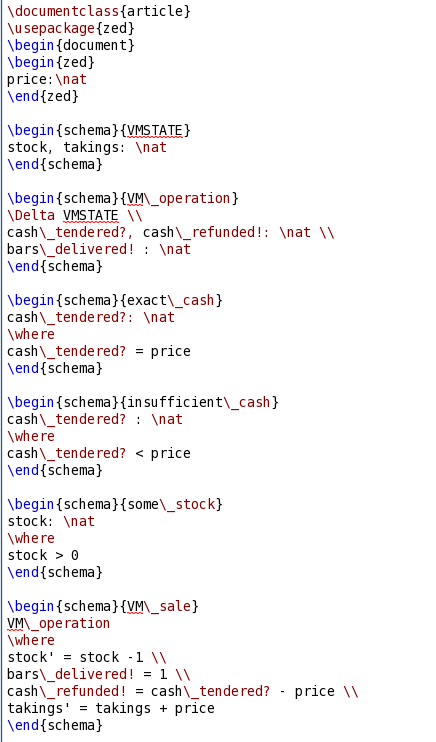
\includegraphics[scale=0.5]{examples/vm/0imagea.png}

\noindent 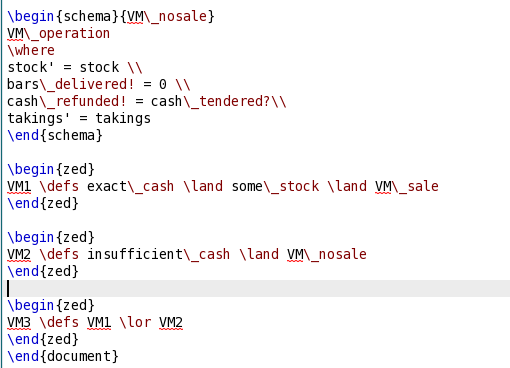
\includegraphics[scale=0.5]{examples/vm/0imageb.png}
\subsection{Raw Latex output}
\label{app:vm0o}

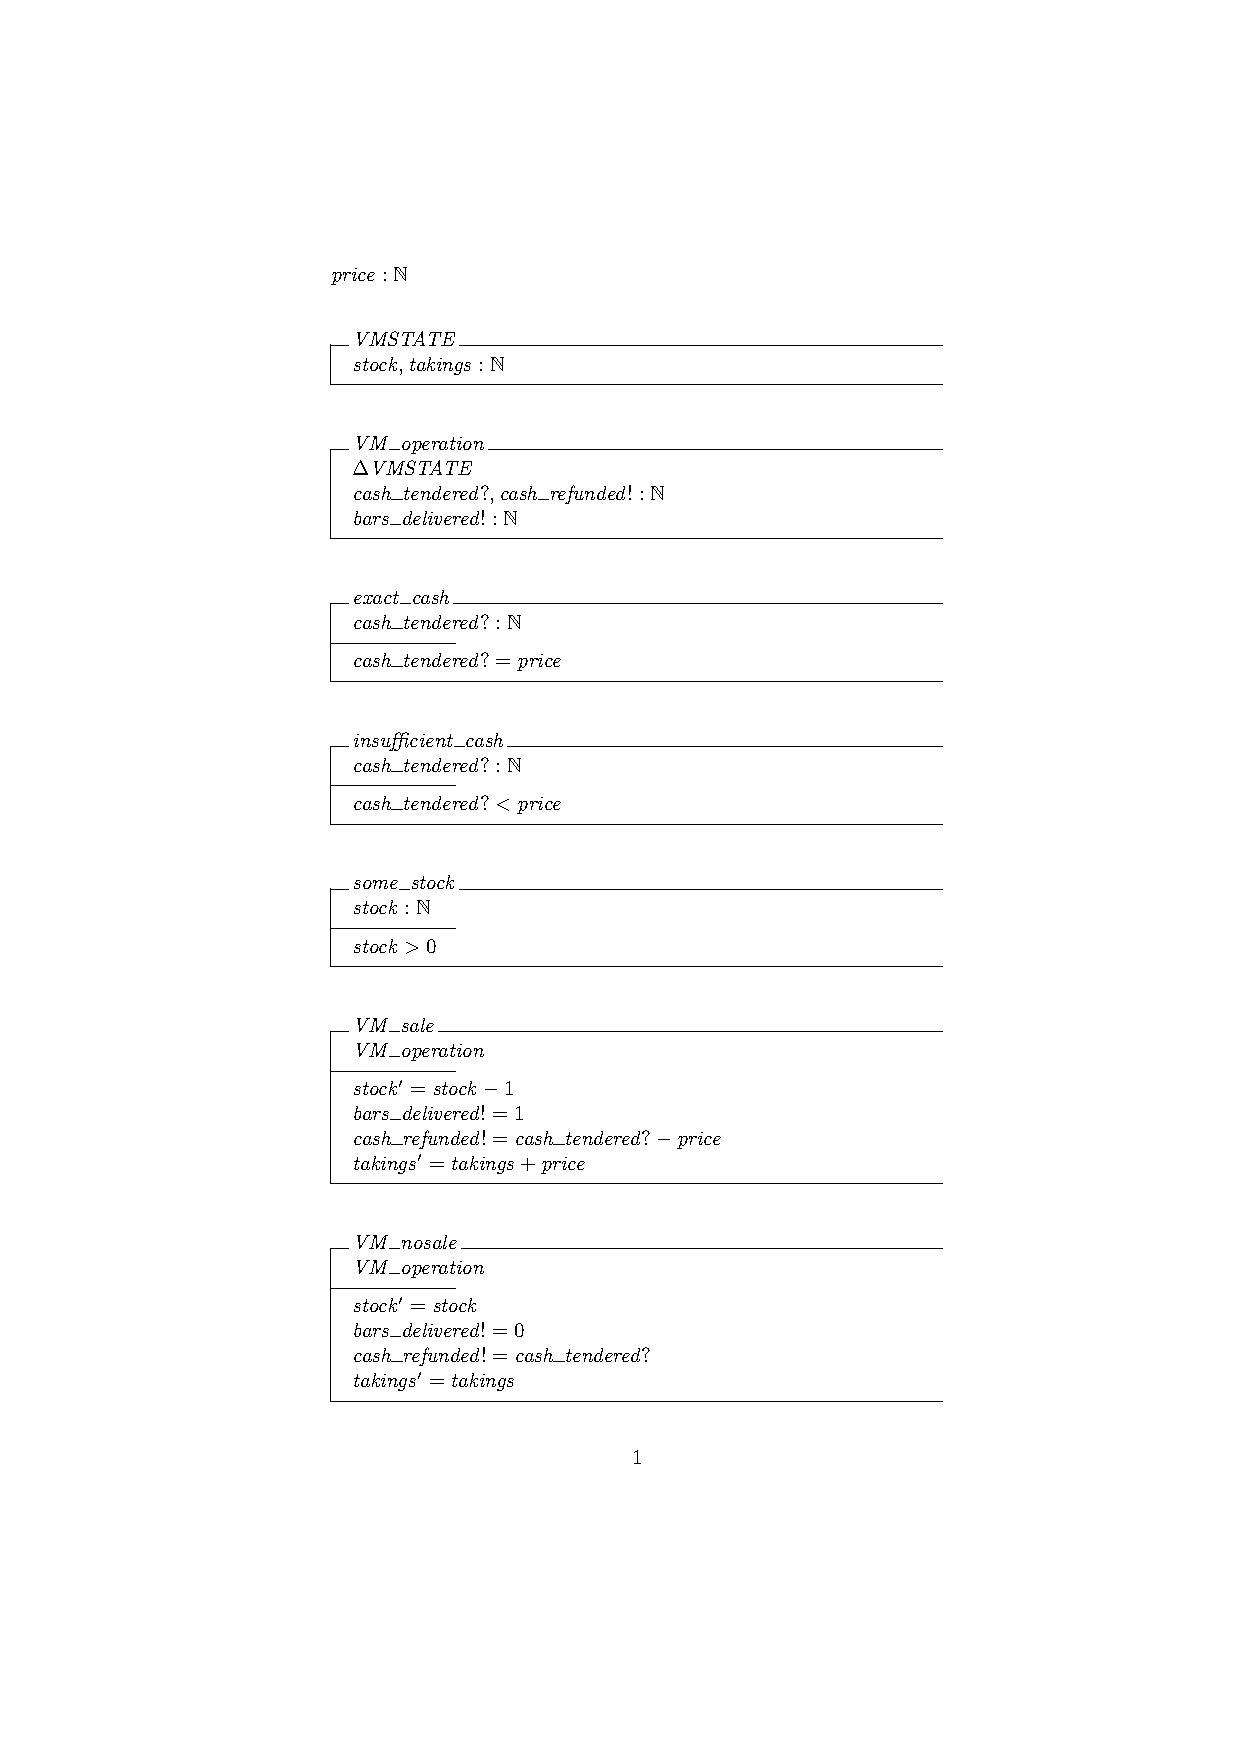
\includegraphics[clip, trim=5cm 5.5cm 5cm 5cm]{examples/vm/0comp.pdf}

\noindent 
\includegraphics[clip, trim=5cm 22cm 5cm 3.5cm]{examples/vm/0comp2.pdf}
%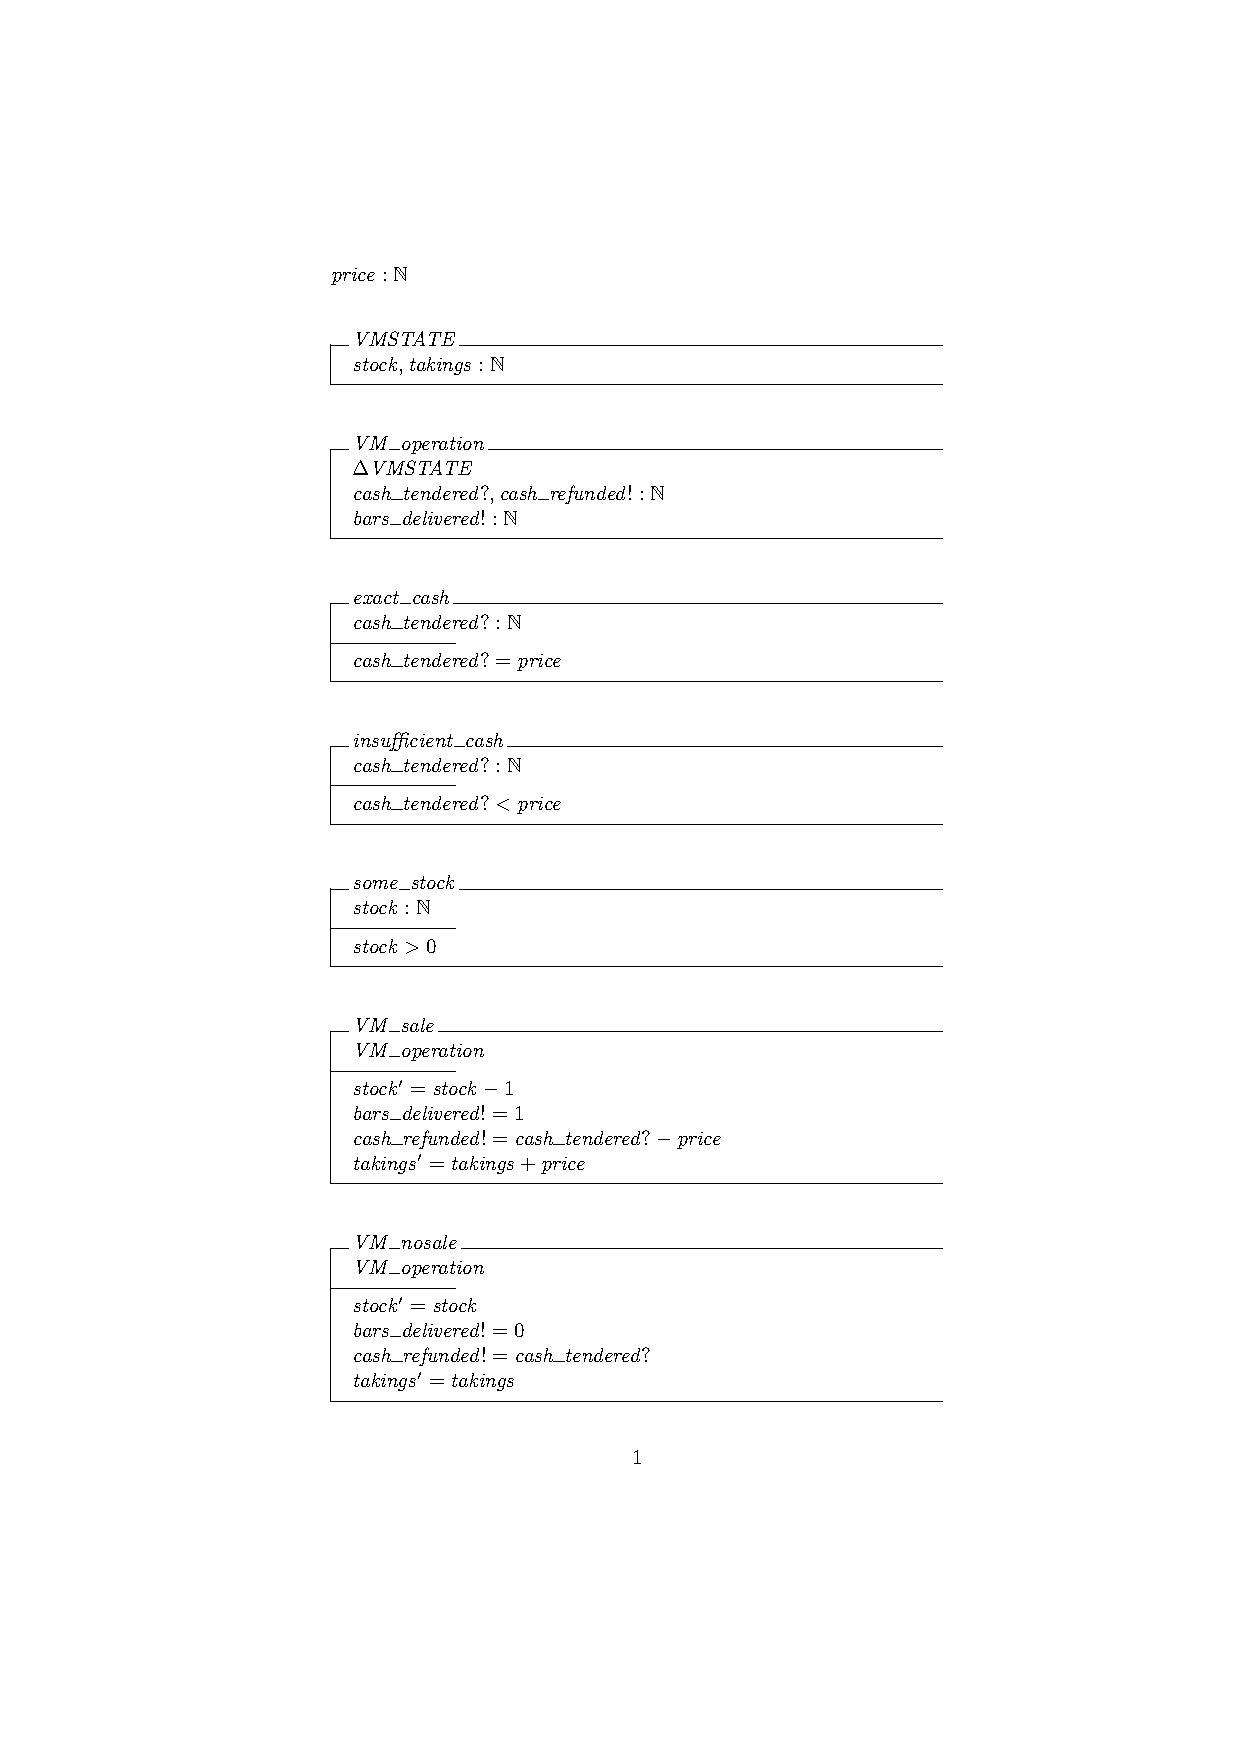
\includepdf[pages={1-2}]{examples/vm/0comp.pdf}
\subsection{ZCGa Annotated Latex Code}
\label{app:vm1}
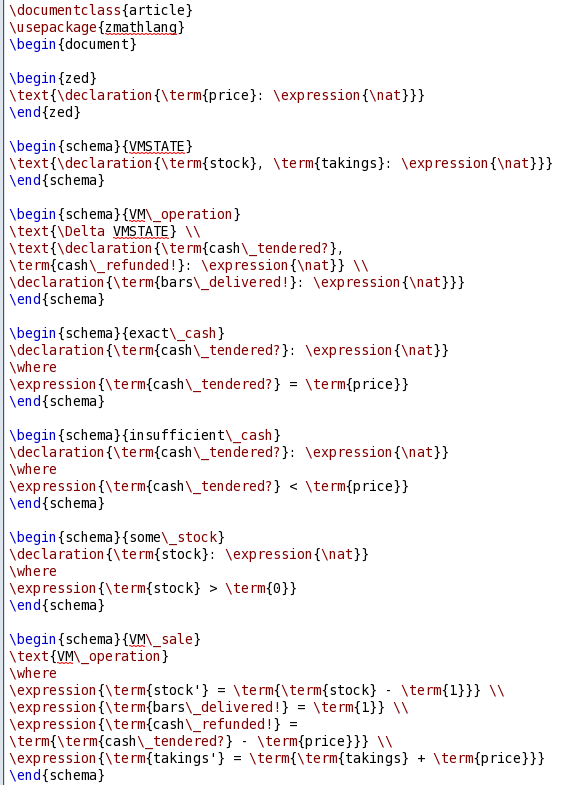
\includegraphics[scale=0.5]{examples/vm/1imagea.png}

\noindent 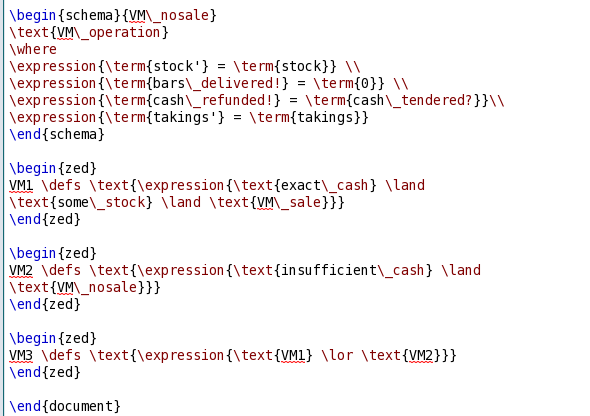
\includegraphics[scale=0.5]{examples/vm/1imageb.png}
%\begin{verbatim}
\documentclass{article}
\usepackage{zmathlang}
\begin{document}
\begin{zed}
\text{\declaration{\term{price}: \expression{\nat}}}
\end{zed}
\begin{schema}{VMSTATE}
\text{\declaration{\term{stock}, \term{takings}: \expression{\nat}}}
\end{schema}
\begin{schema}{VM\_operation}
\text{\Delta VMSTATE} \\
\text{\declaration{\term{cash\_tendered?},
\term{cash\_refunded!}: \expression{\nat}} \\
\declaration{\term{bars\_delivered!}: \expression{\nat}}}
\end{schema}
\begin{schema}{exact\_cash}
\declaration{\term{cash\_tendered?}: \expression{\nat}}
\where
\expression{\term{cash\_tendered?} = \term{price}}
\end{schema}
\begin{schema}{insufficient\_cash}
\declaration{\term{cash\_tendered?}: \expression{\nat}}
\where
\expression{\term{cash\_tendered?} < \term{price}}
\end{schema}
\begin{schema}{some\_stock}
\declaration{\term{stock}: \expression{\nat}}
\where
\expression{\term{stock} > \term{0}}
\end{schema}
\begin{schema}{VM\_sale}
\text{VM\_operation}
\where
\expression{\term{stock'} = \term{\term{stock} - \term{1}}} \\
\expression{\term{bars\_delivered!} = \term{1}} \\
\expression{\term{cash\_refunded!} =
\term{\term{cash\_tendered?} - \term{price}}} \\
\expression{\term{takings'} = \term{\term{takings} + \term{price}}}
\end{schema}
\begin{schema}{VM\_nosale}
\text{VM\_operation}
\where
\expression{\term{stock'} = \term{stock}} \\
\expression{\term{bars\_delivered!} = \term{0}} \\
\expression{\term{cash\_refunded!} = \term{cash\_tendered?}}\\
\expression{\term{takings'} = \term{takings}}
\end{schema}
\begin{zed}
VM1 \defs \text{\expression{\text{exact\_cash} \land
\text{some\_stock} \land \text{VM\_sale}}}
\end{zed}
\begin{zed}
VM2 \defs \text{\expression{\text{insufficient\_cash} \land
\text{VM\_nosale}}}
\end{zed}
\begin{zed}
VM3 \defs \text{\expression{\text{VM1} \lor \text{VM2}}}
\end{zed}
\end{document}
\end{verbatim}
\subsection{ZCGa output}
\label{app:vm1o}
%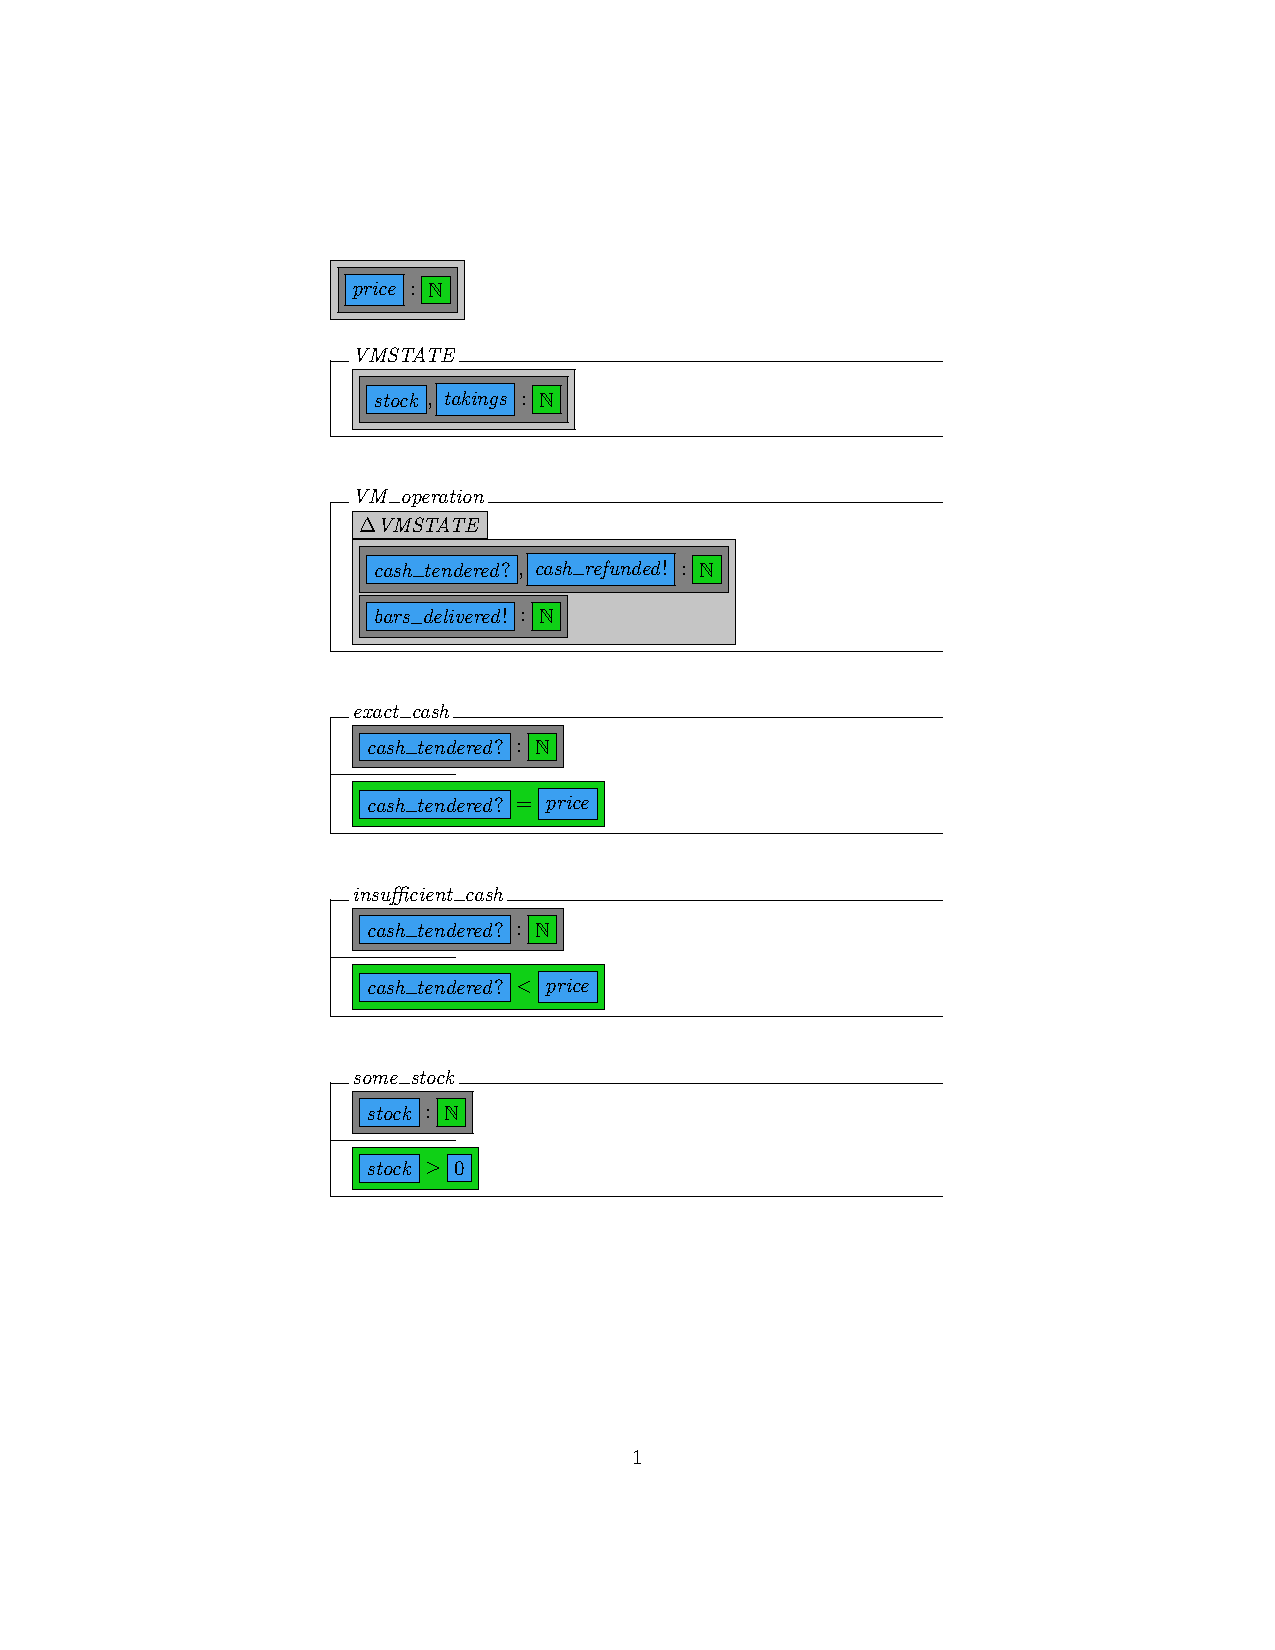
\includegraphics[clip, trim=5cm 7cm 5cm 4.2cm]{examples/vm/1comp.pdf}
%\noindent 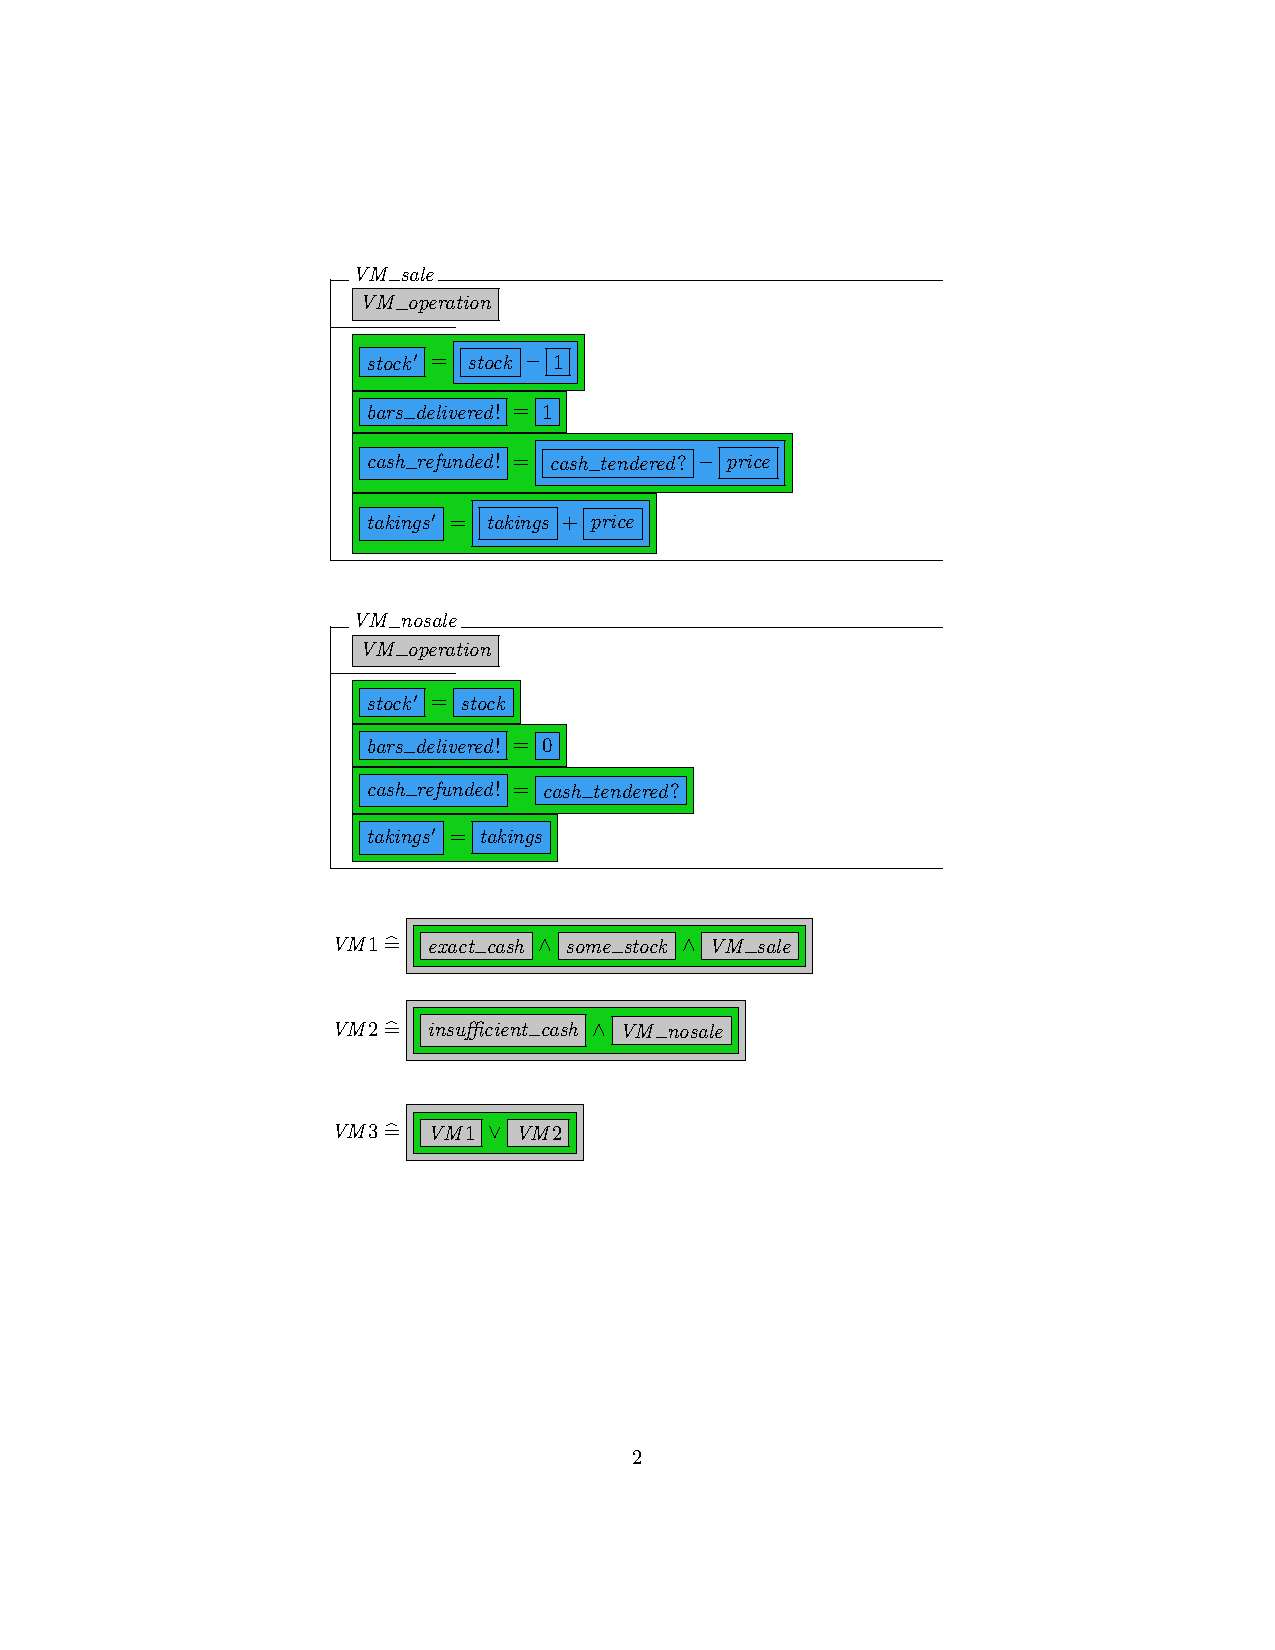
\includegraphics[clip, trim=4cm 7cm 5cm 4cm]{examples/vm/1comp2.pdf}

\begin{figure}[H]
    \hfill
    \subfigure{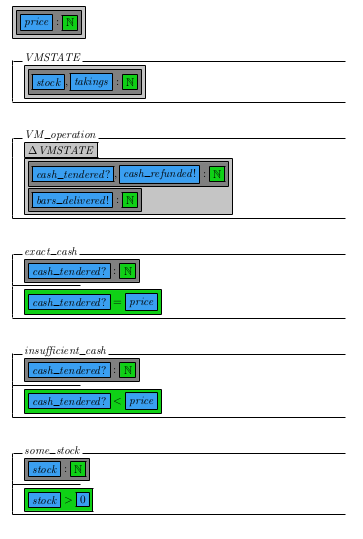
\includegraphics[width=8cm]{Figures/appendix/vmzcgao1.png}}
    \hfill
    \subfigure{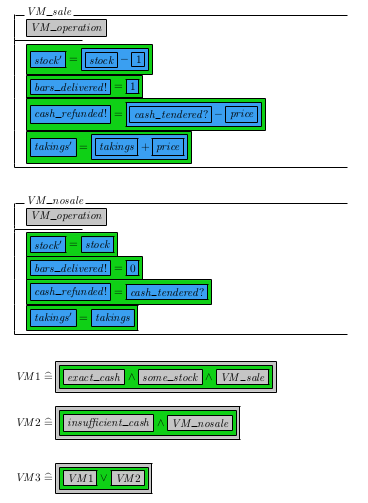
\includegraphics[width=8cm]{Figures/appendix/vmzvgao2.png}}
    \hfill
\end{figure}


\subsection{ZDRa Annotated Latex Code}
\label{app:vm2}
%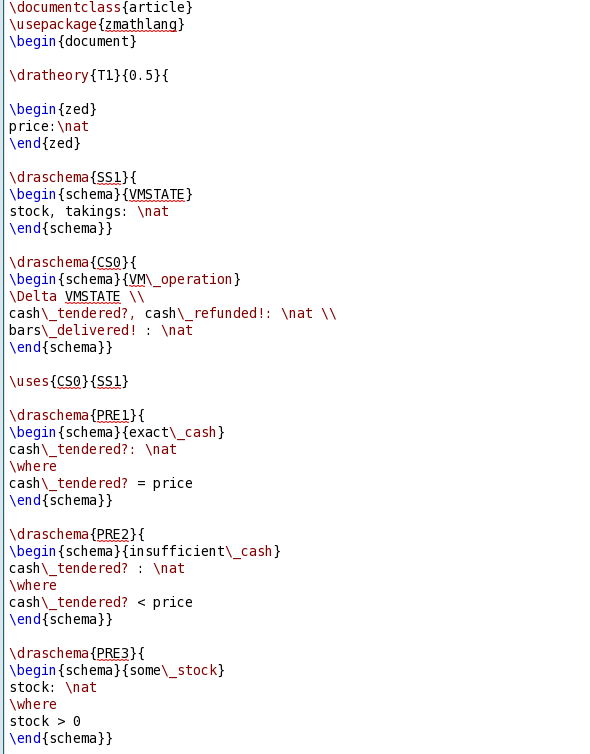
\includegraphics[scale=0.5]{examples/vm/2imagea.png}

\begin{figure}[H]
    \hfill
    \subfigure{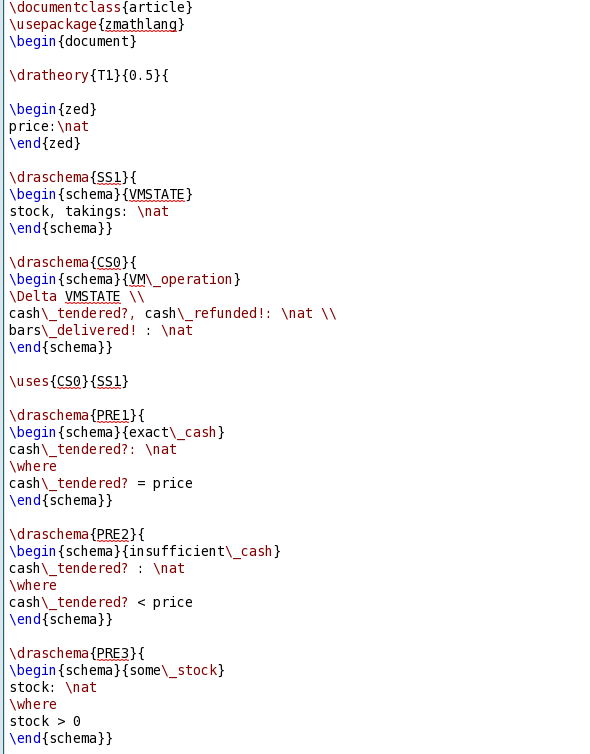
\includegraphics[width=9cm]{examples/vm/2imagea.png}}
    \hfill
    \subfigure{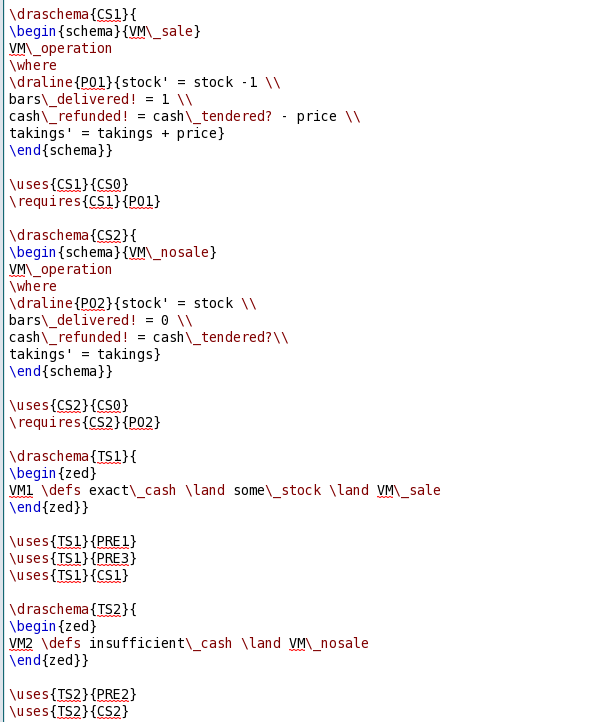
\includegraphics[width=9cm]{examples/vm/2imageb.png}}
    \hfill
\end{figure}

\begin{figure}[H]
    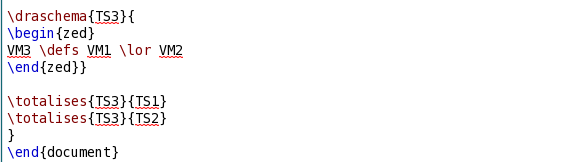
\includegraphics[width=7cm]{examples/vm/2imagec.png}
\end{figure}

%\noindent 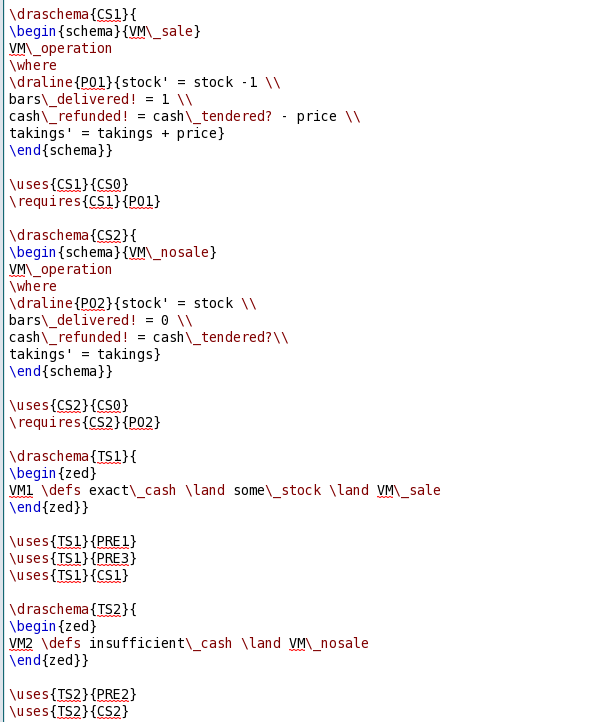
\includegraphics[scale=0.5]{examples/vm/2imageb.png}
%\noindent 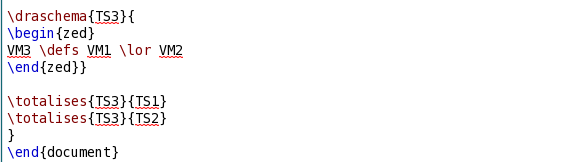
\includegraphics[scale=0.5]{examples/vm/2imagec.png}

\subsection{ZDRa Output}
\label{app:vm2o}

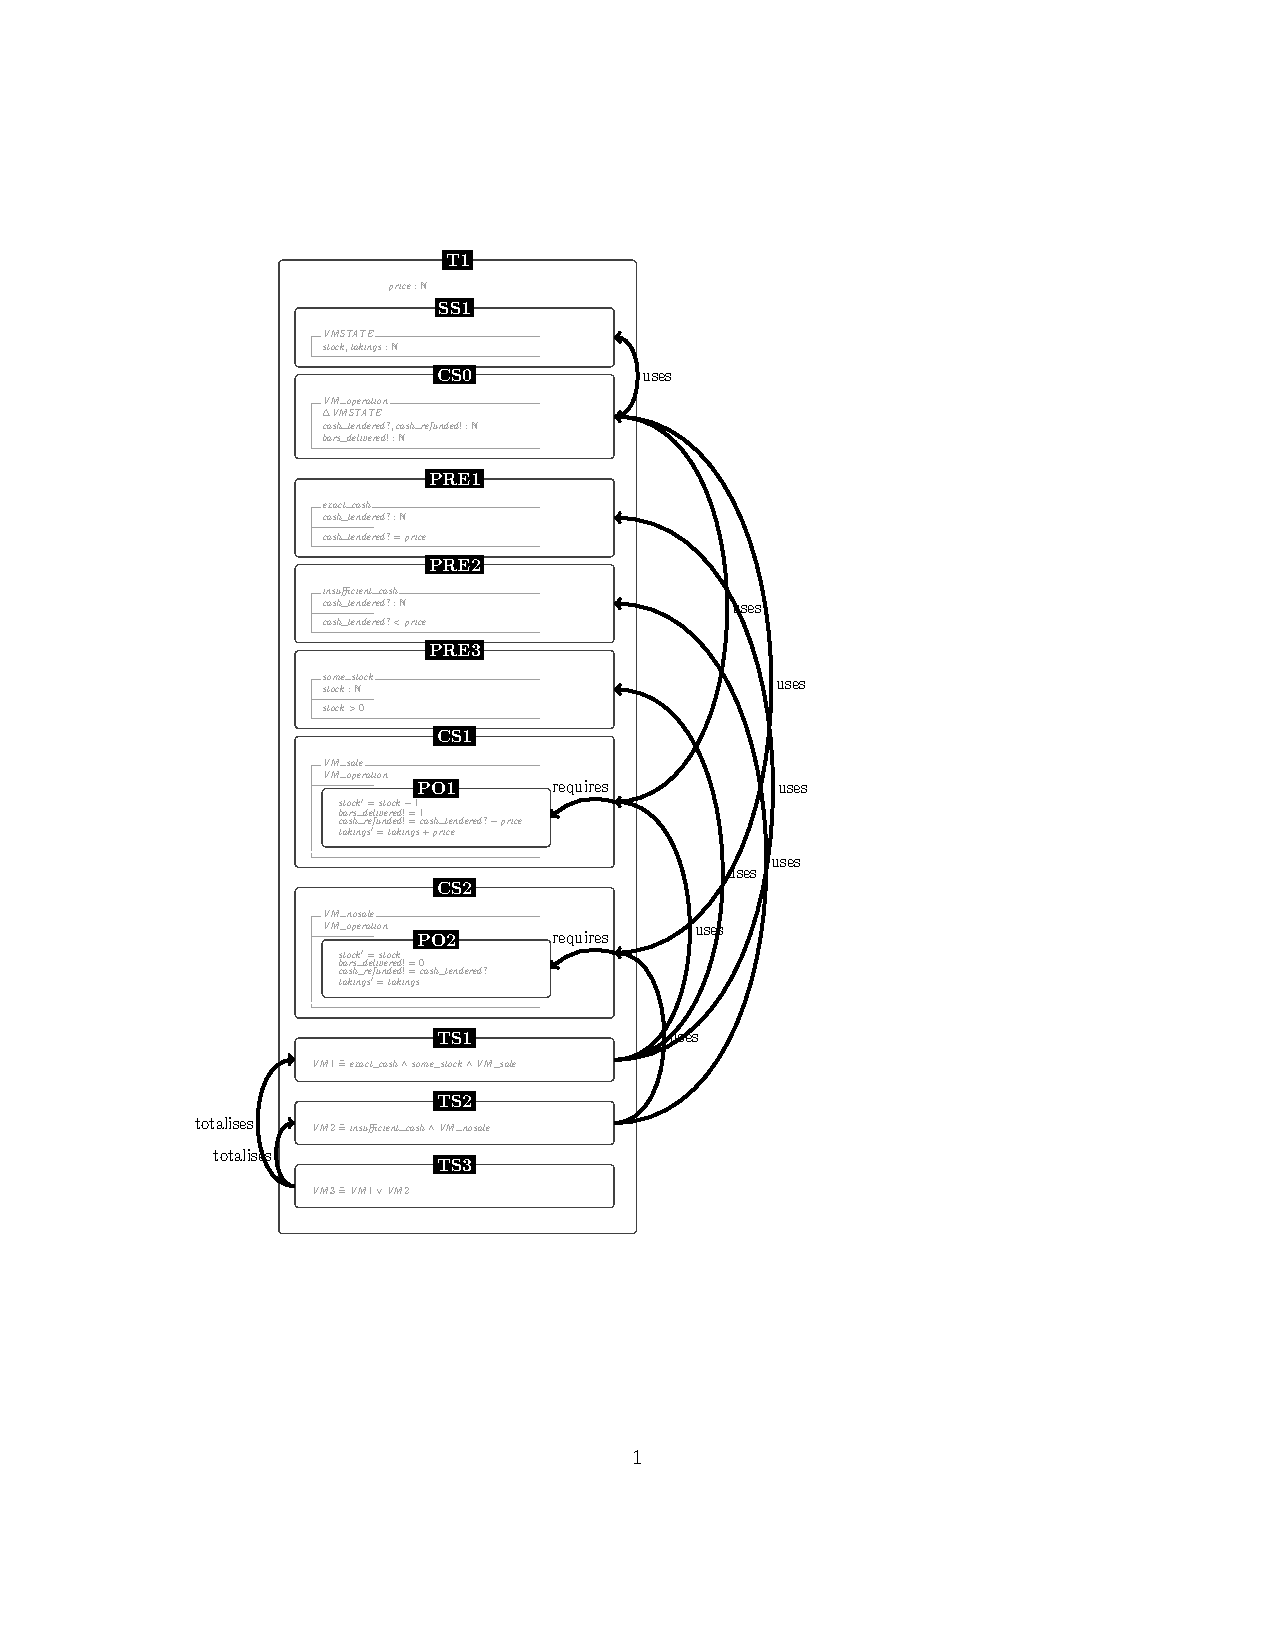
\includegraphics[clip, trim=3cm 7cm 6cm 4.2cm]{examples/vm/2comp.pdf}

%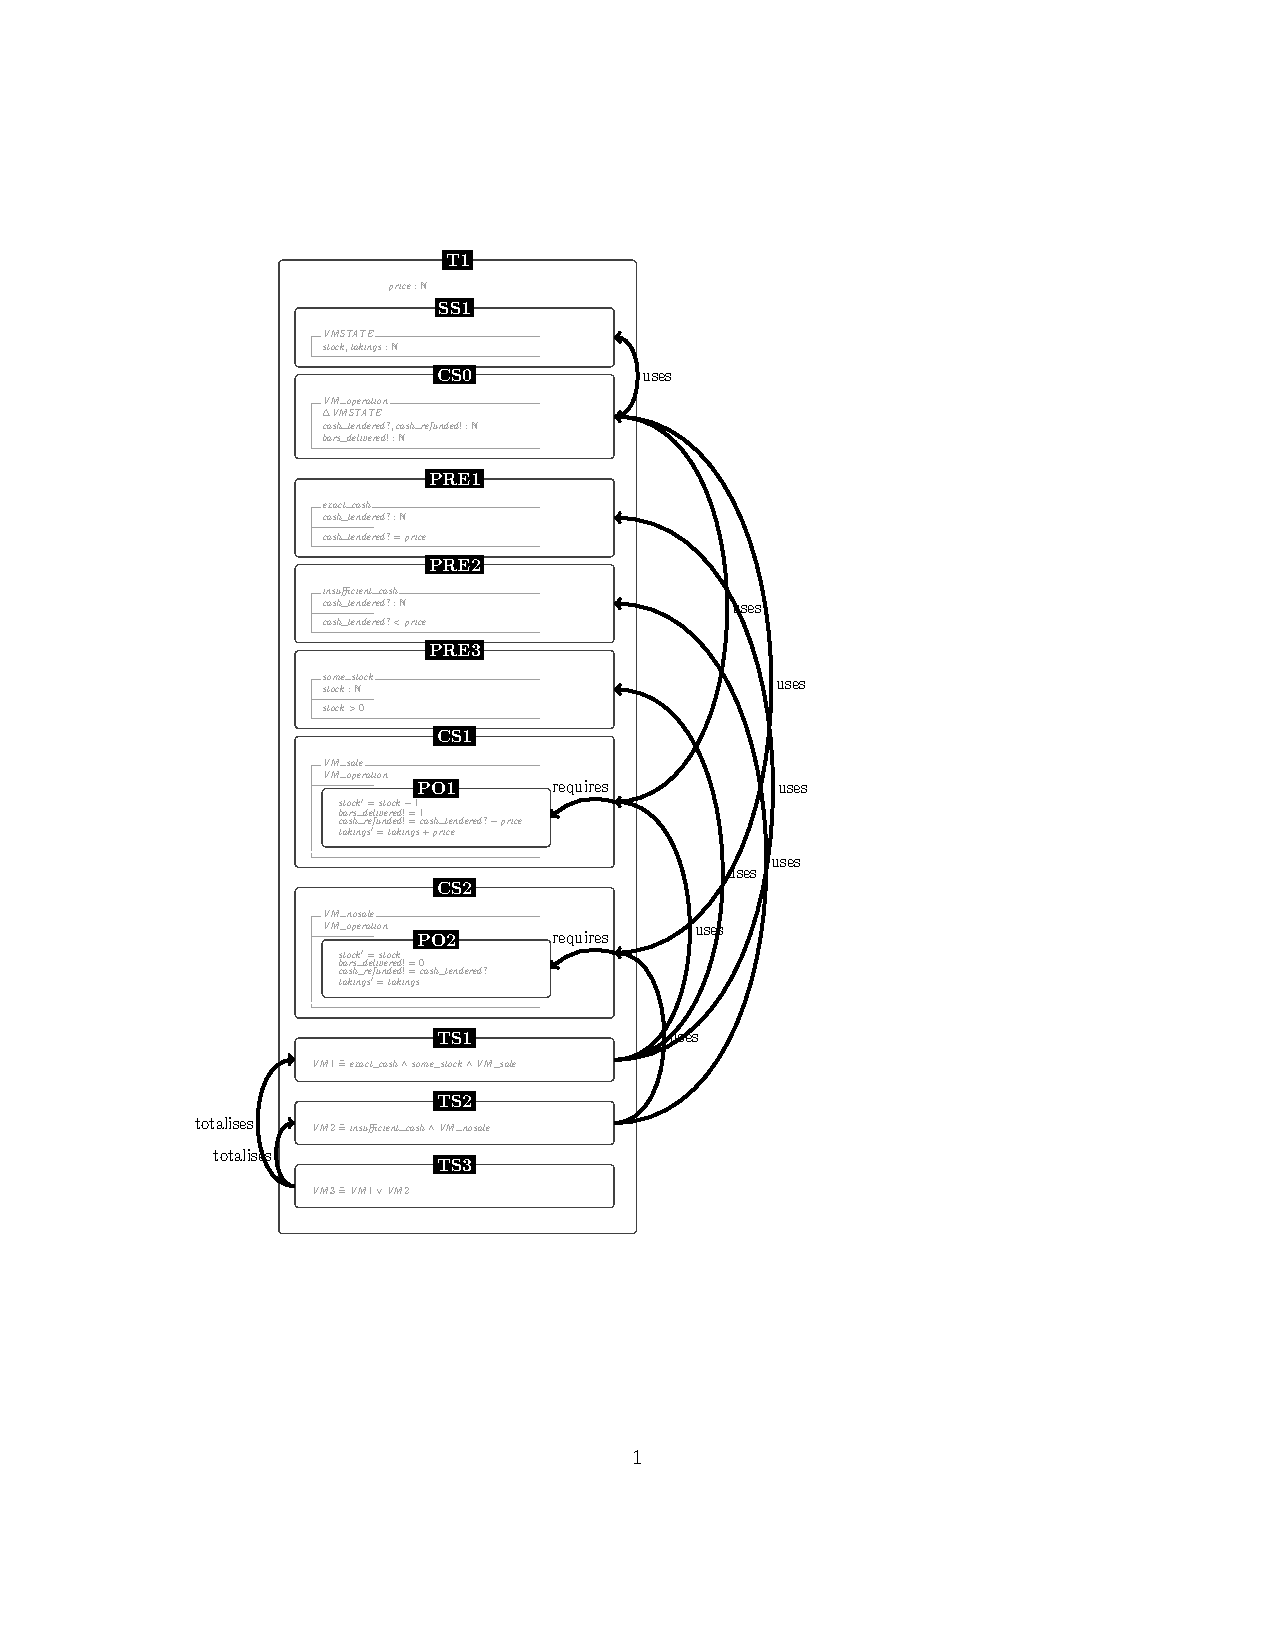
\includepdf[pages={1}]{examples/vm/2comp.pdf}
\subsection{ZCGa and ZDRa Annotated Latex Code}
\label{app:vm1n2}
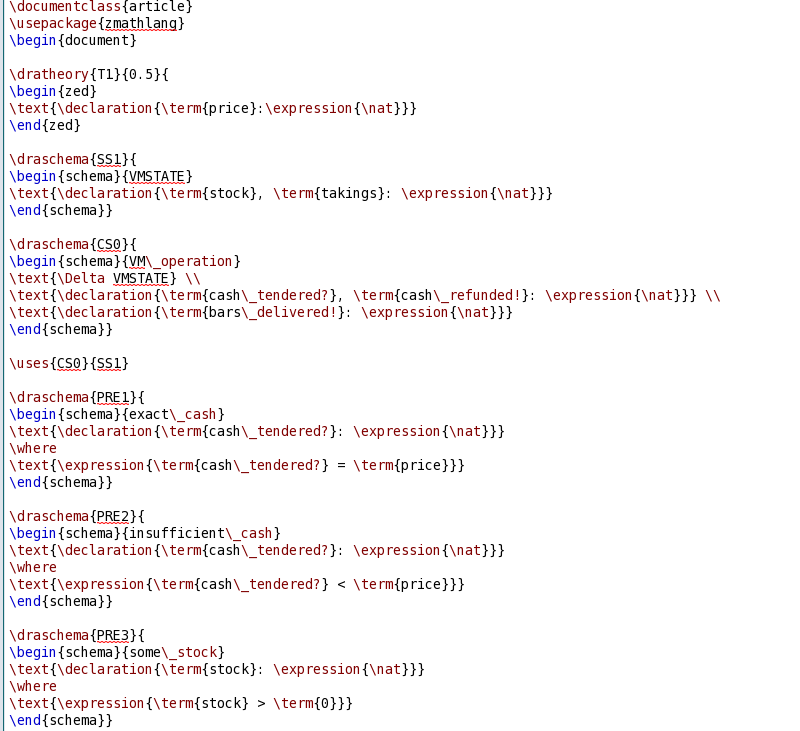
\includegraphics[scale=0.5]{examples/vm/1n2imagea.png}

\noindent 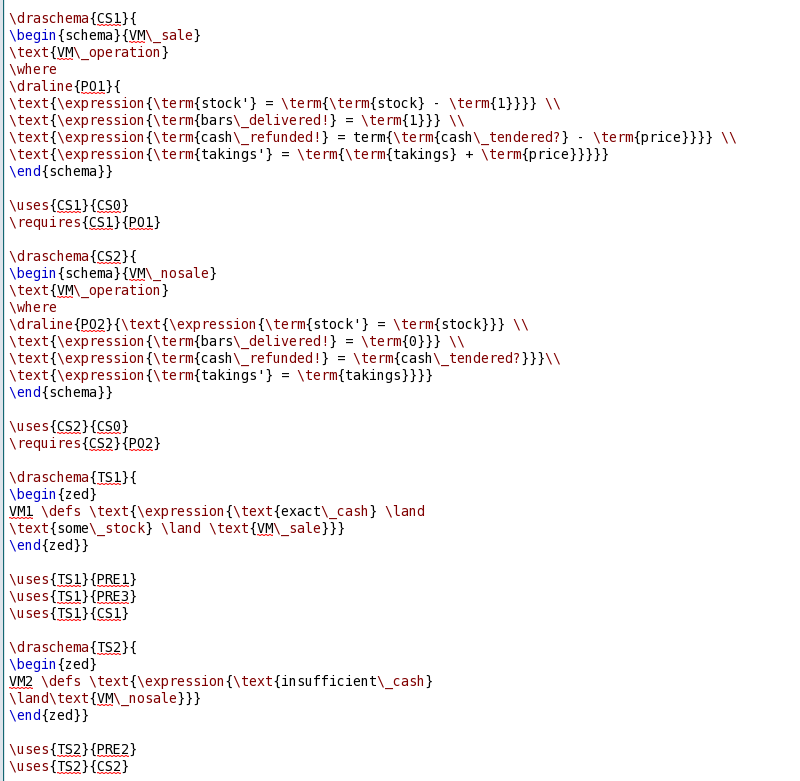
\includegraphics[scale=0.5]{examples/vm/1n2imageb.png}

\noindent 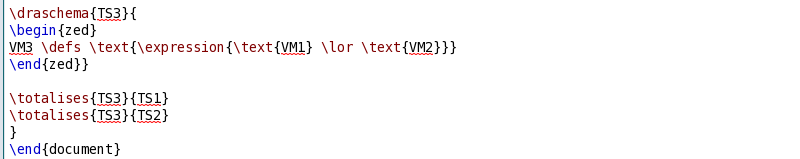
\includegraphics[scale=0.5]{examples/vm/1n2imagec.png}

%\begin{verbatim}
\documentclass{article}
\usepackage{zmathlang}
\begin{document}
\dratheory{T1}{0.5}{
\begin{zed}
\text{\declaration{\term{price}:\expression{\nat}}}
\end{zed}
\draschema{SS1}{
\begin{schema}{VMSTATE}
\text{\declaration{\term{stock},
\term{takings}: \expression{\nat}}}
\end{schema}}
\draschema{CS0}{
\begin{schema}{VM\_operation}
\text{\Delta VMSTATE} \\
\text{\declaration{\term{cash\_tendered?},
\term{cash\_refunded!}: \expression{\nat}}} \\
\text{\declaration{\term{bars\_delivered!}:
\expression{\nat}}}
\end{schema}}
\uses{CS0}{SS1}
\draschema{PRE1}{
\begin{schema}{exact\_cash}
\text{\declaration{\term{cash\_tendered?}:
\expression{\nat}}}
\where
\text{\expression{\term{cash\_tendered?} =
\term{price}}}
\end{schema}}
\draschema{PRE2}{
\begin{schema}{insufficient\_cash}
\text{\declaration{\term{cash\_tendered?}: 
\expression{\nat}}}
\where
\text{\expression{\term{cash\_tendered?} <
\term{price}}}
\end{schema}}
\draschema{PRE3}{
\begin{schema}{some\_stock}
\text{\declaration{\term{stock}: \expression{\nat}}}
\where
\text{\expression{\term{stock} > \term{0}}}
\end{schema}}
\draschema{CS1}{
\begin{schema}{VM\_sale}
\text{VM\_operation}
\where
\draline{PO1}{
\text{\expression{\term{stock'} = 
\term{\term{stock} - \term{1}}}} \\
\text{\expression{\term{bars\_delivered!} =
\term{1}}} \\
\text{\expression{\term{cash\_refunded!} =
term{\term{cash\_tendered?} - \term{price}}}} \\
\text{\expression{\term{takings'} =
\term{\term{takings} + \term{price}}}}}
\end{schema}}
\uses{CS1}{CS0}
\requires{CS1}{PO1}
\draschema{CS2}{
\begin{schema}{VM\_nosale}
\text{VM\_operation}
\where
\draline{PO2}{\text{\expression{\term{stock'} =
\term{stock}}} \\
\text{\expression{\term{bars\_delivered!} =
\term{0}}} \\
\text{\expression{\term{cash\_refunded!} =
\term{cash\_tendered?}}}\\
\text{\expression{\term{takings'} =
\term{takings}}}}
\end{schema}}
\uses{CS2}{CS0}
\requires{CS2}{PO2}
\draschema{TS1}{
\begin{zed}
VM1 \defs \text{\expression{\text{exact\_cash} \land
\text{some\_stock} \land \text{VM\_sale}}}
\end{zed}}
\uses{TS1}{PRE1}
\uses{TS1}{PRE3}
\uses{TS1}{CS1}
\draschema{TS2}{
\begin{zed}
VM2 \defs \text{\expression{\text{insufficient\_cash}
\land\text{VM\_nosale}}}
\end{zed}}
\uses{TS2}{PRE2}
\uses{TS2}{CS2}
\draschema{TS3}{
\begin{zed}
VM3 \defs \text{\expression{\text{VM1} \lor \text{VM2}}}
\end{zed}}
\totalises{TS3}{TS1}
\totalises{TS3}{TS2}
}
\end{document}
\end{verbatim}
\subsection{ZCGa and ZDRa Output}
\label{app:vm1n2o}
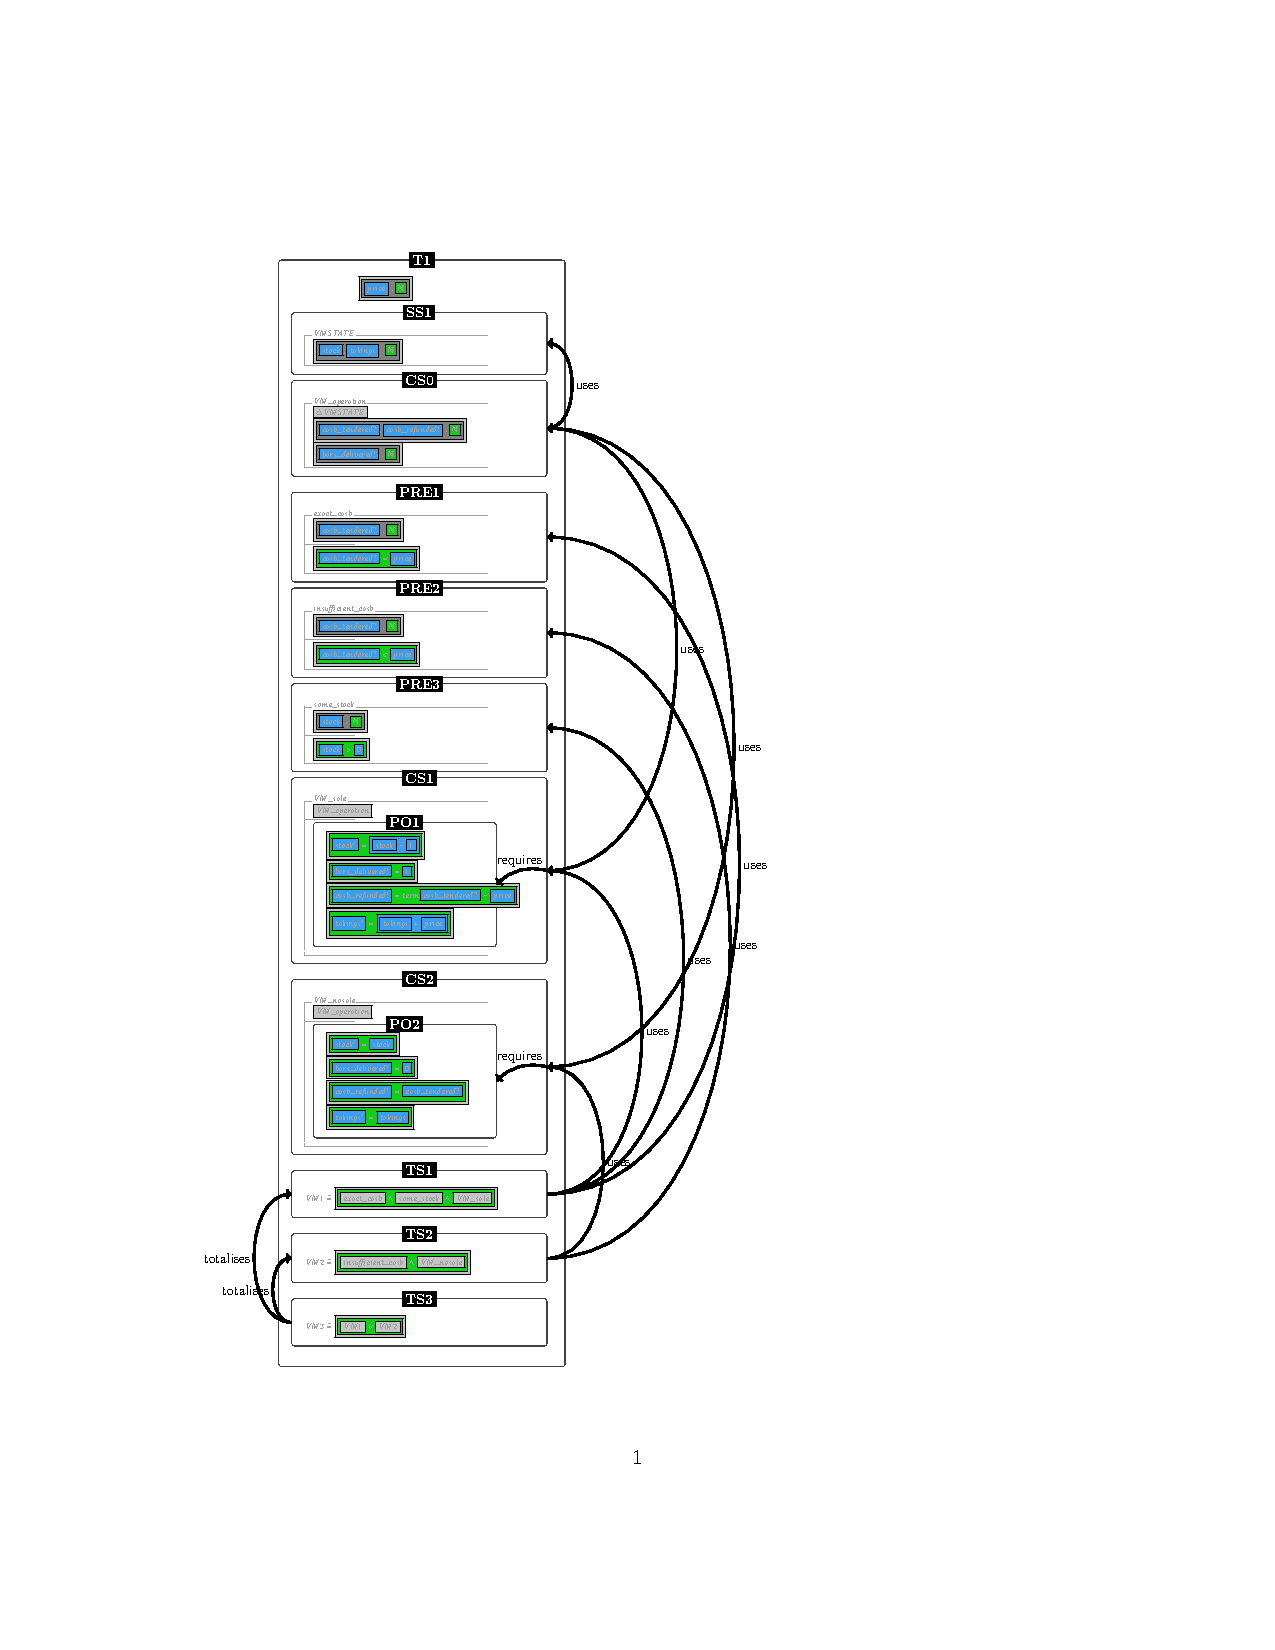
\includegraphics[clip, trim=3cm 4cm 6cm 4.2cm]{examples/vm/1n2comp.pdf}
%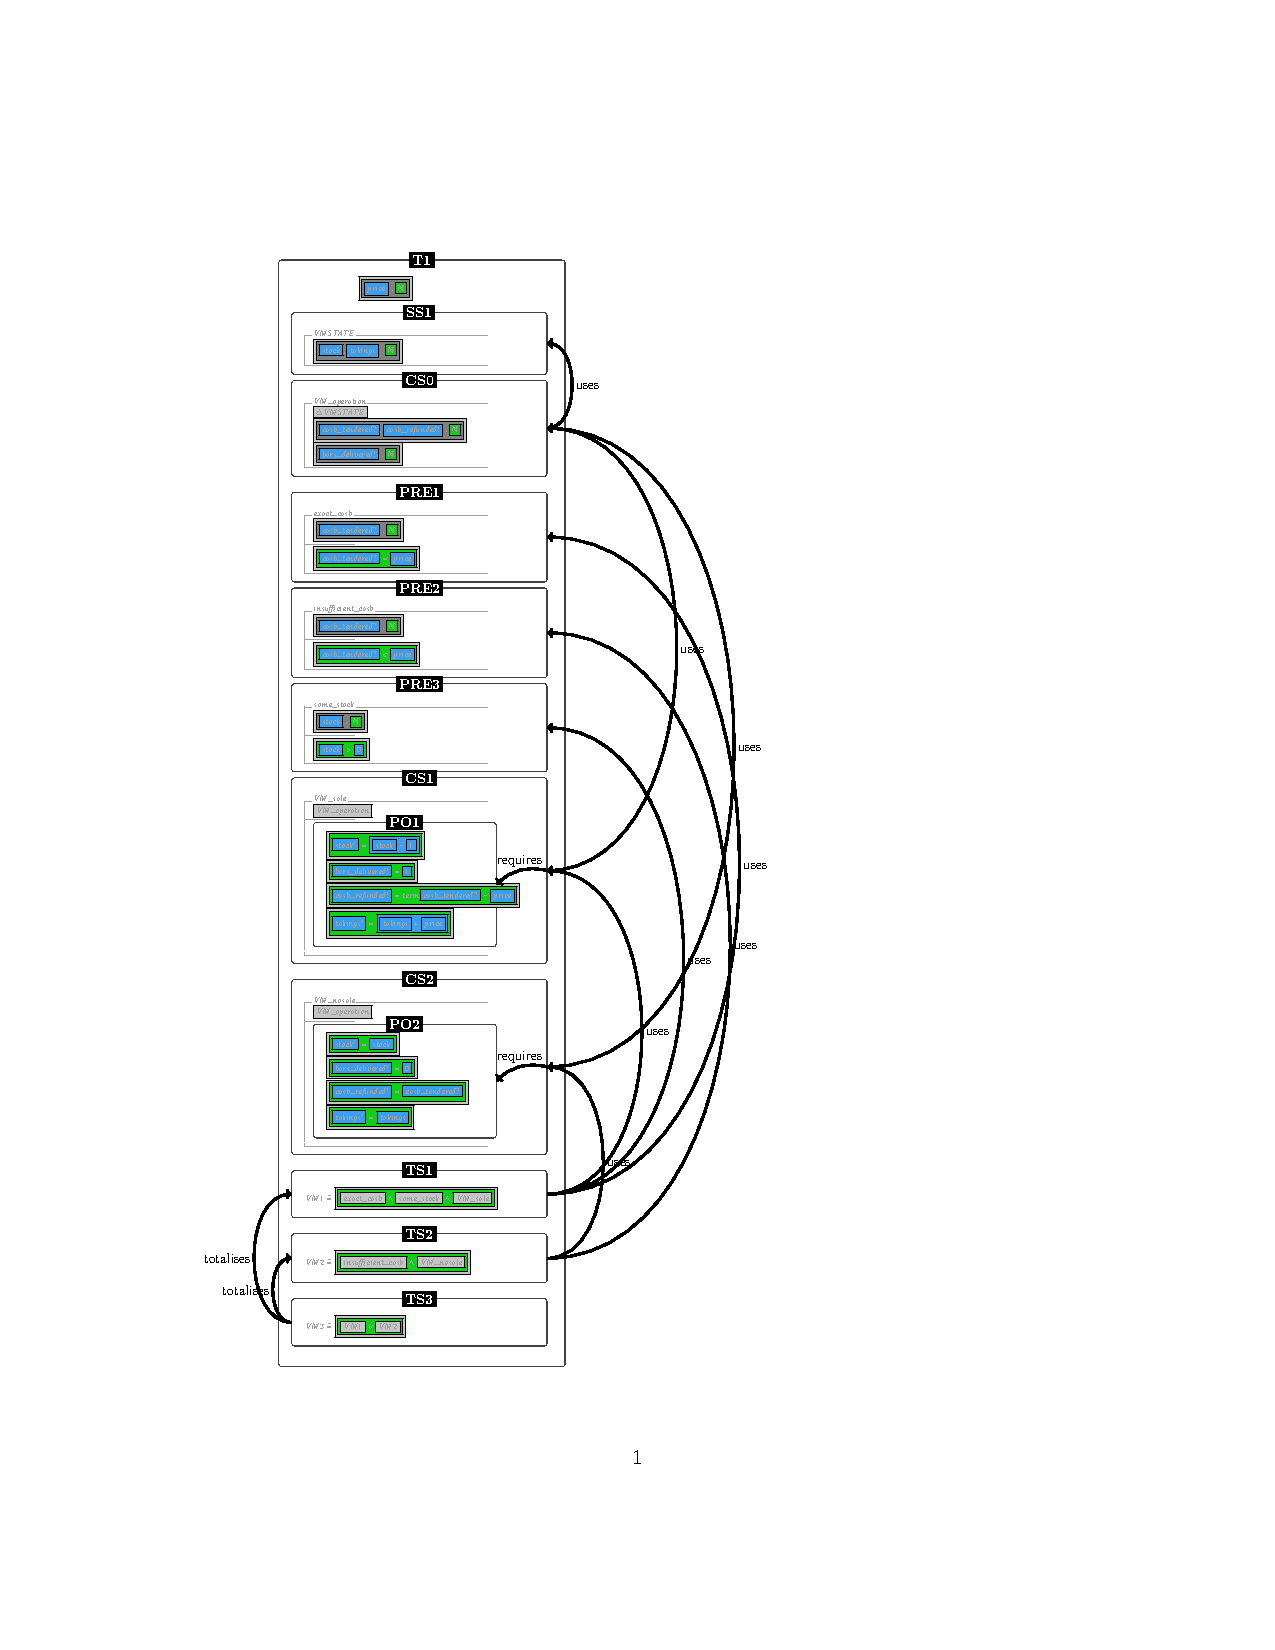
\includepdf[pages={1}]{examples/vm/1n2comp.pdf}
\subsection{Dependency and Goto Graphs}
\label{app:vm2.5}
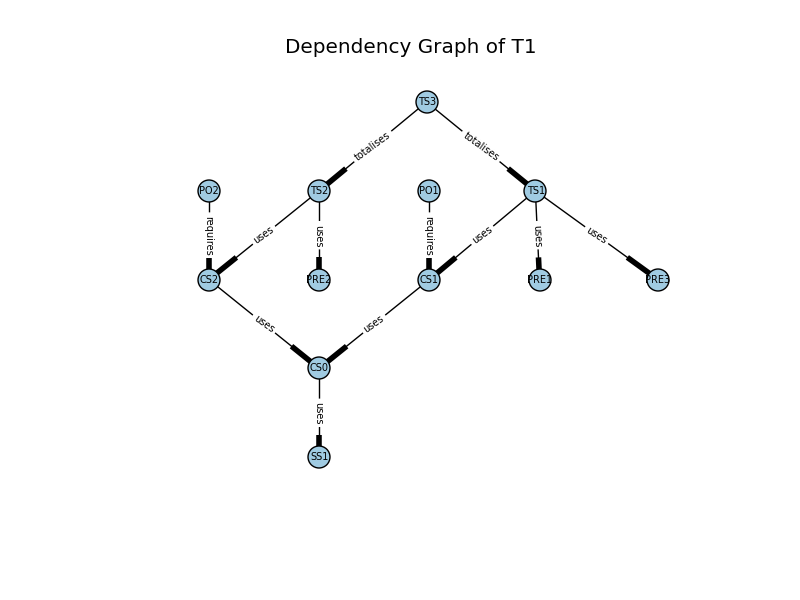
\includegraphics[scale=0.7]{examples/vm/25a.png}

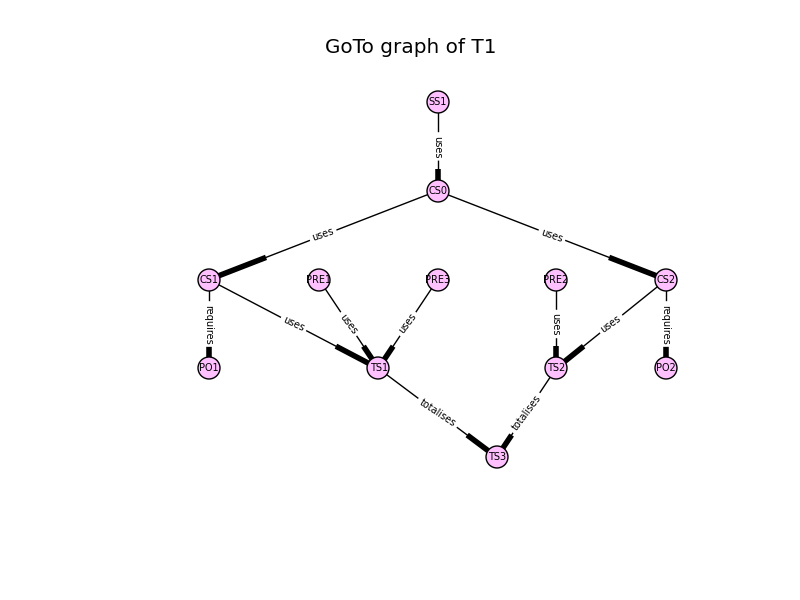
\includegraphics[scale=0.7]{examples/vm/25b.png}
\subsection{General Proof Skeleton}
\label{app:vm3}
\input{examples/vm/3.txt}

\subsection{Isabelle Proof Skeleton}
\label{app:vm4}
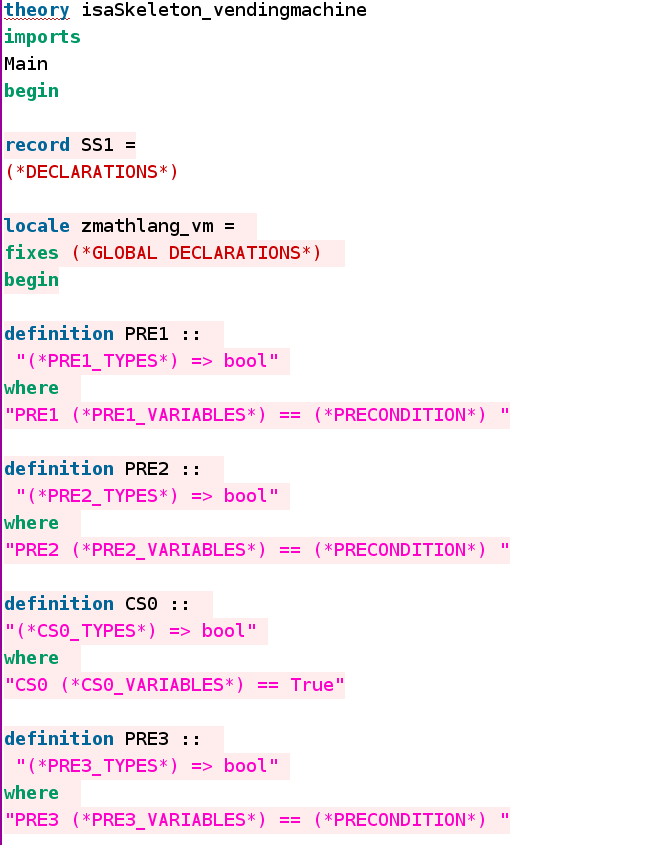
\includegraphics[scale=0.5]{examples/vm/4imagea.png}

\noindent 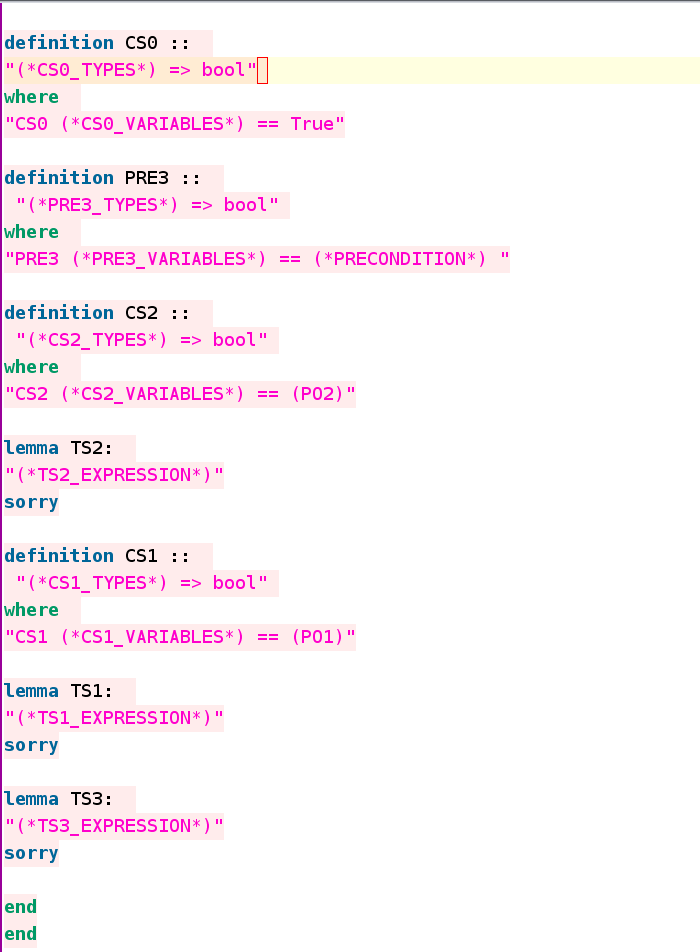
\includegraphics[scale=0.5]{examples/vm/4imageb.png}
%\input{examples/vm/4.thy}
\subsection{Isabelle Filled In}
\label{app:vm5}
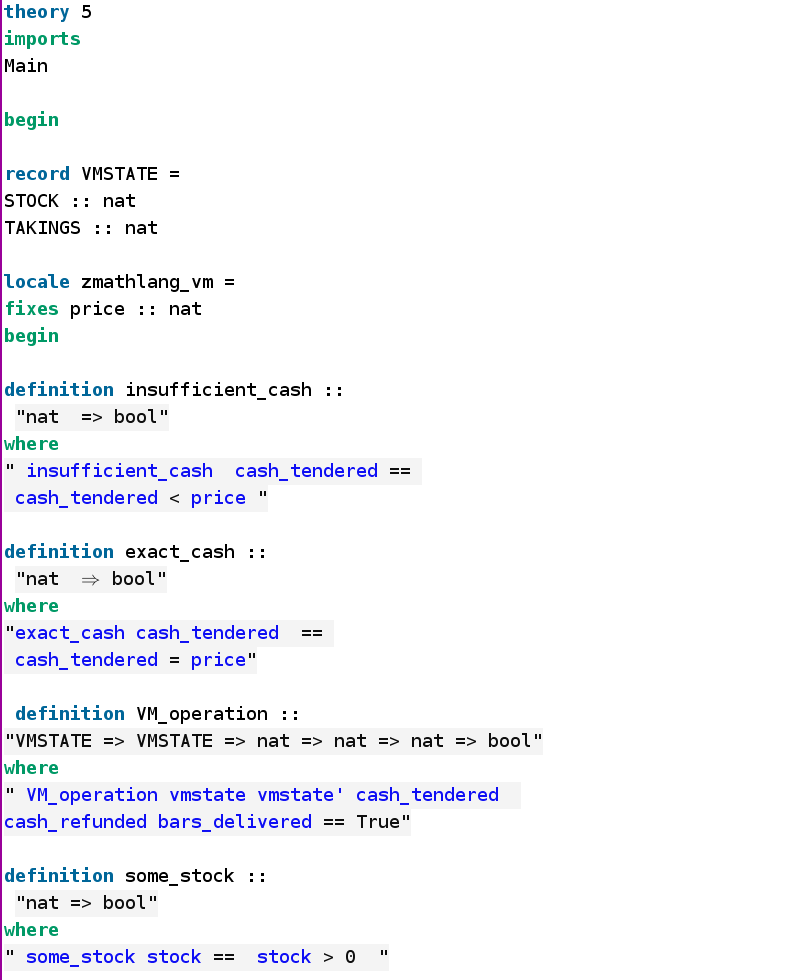
\includegraphics[scale=0.5]{examples/vm/5imagea.png}

\noindent 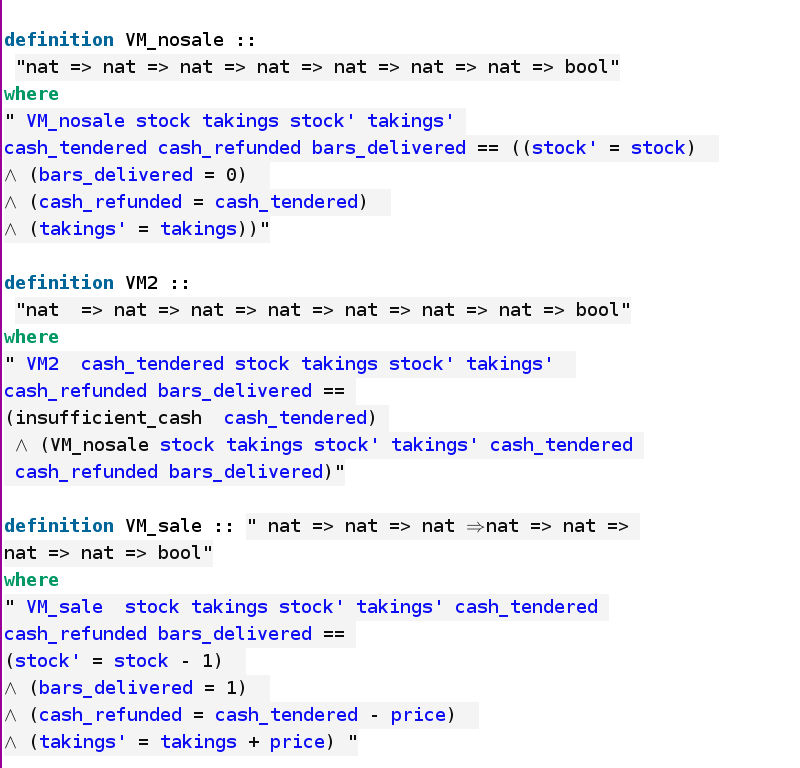
\includegraphics[scale=0.5]{examples/vm/5imageb.png}

\noindent 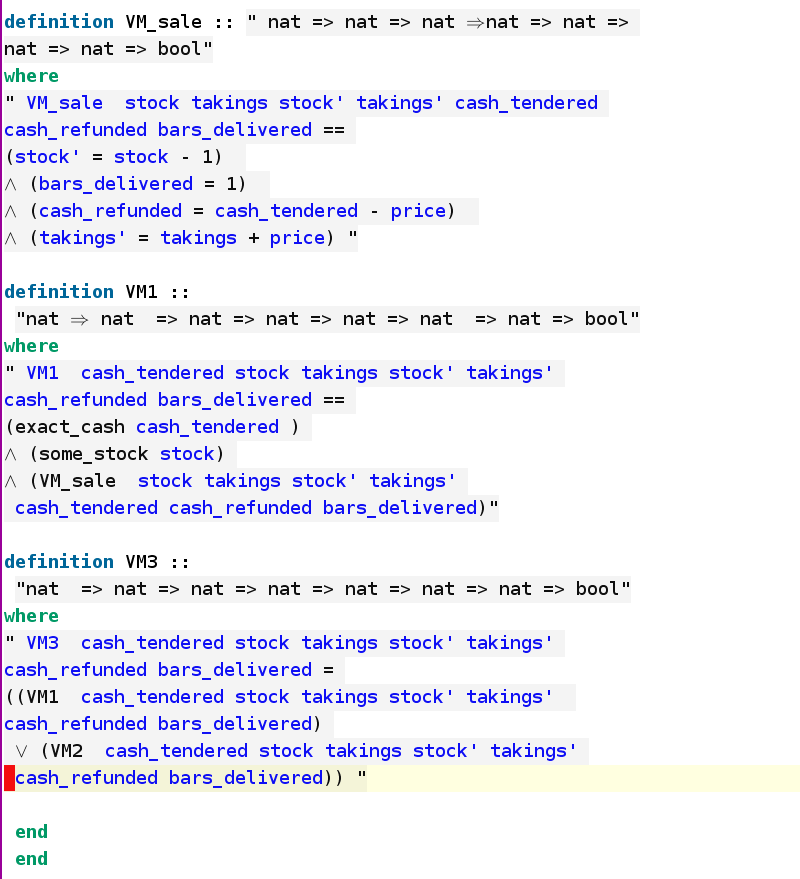
\includegraphics[scale=0.5]{examples/vm/5imagec.png}
%\input{examples/vm/5.thy}
\subsection{Full Proof in Isabelle}
\label{app:vm6}
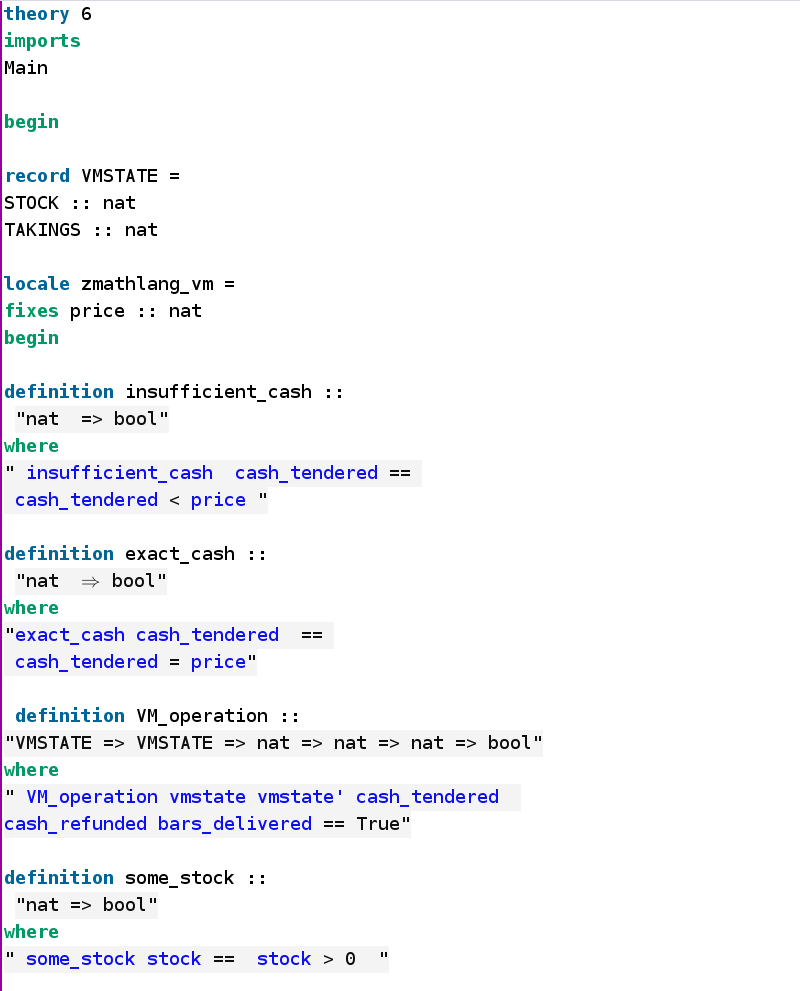
\includegraphics[scale=0.5]{examples/vm/6imagea.png}

\noindent 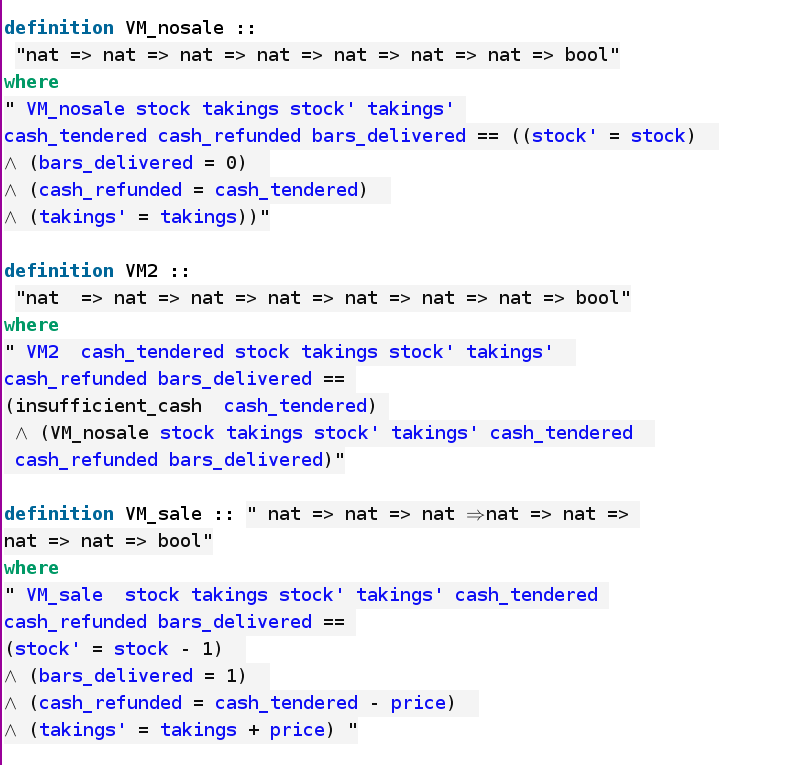
\includegraphics[scale=0.5]{examples/vm/6imageb.png}

\noindent 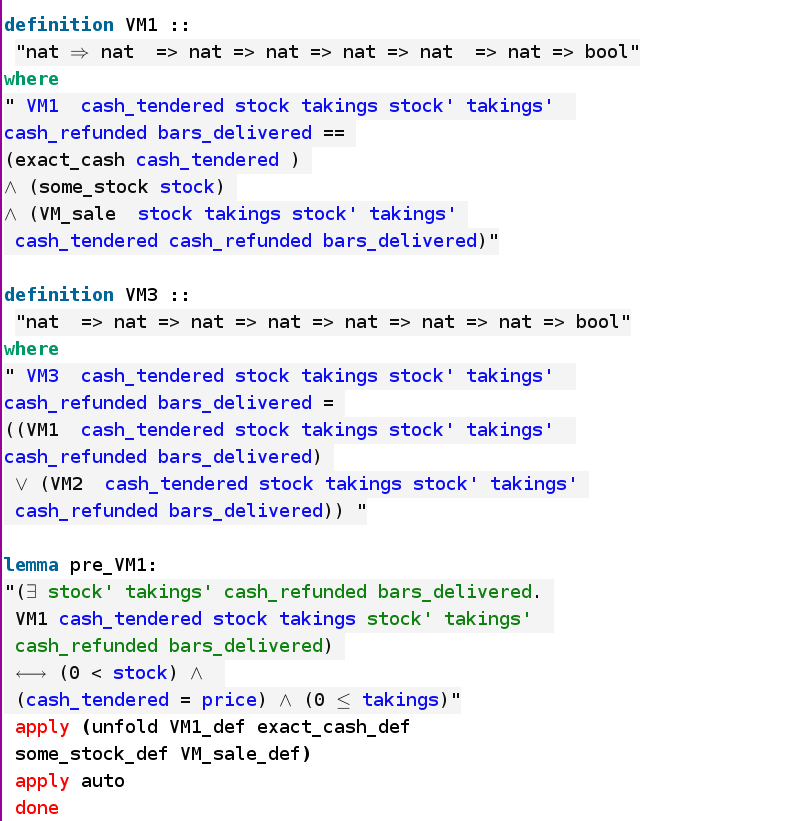
\includegraphics[scale=0.5]{examples/vm/6imagec.png}

\noindent 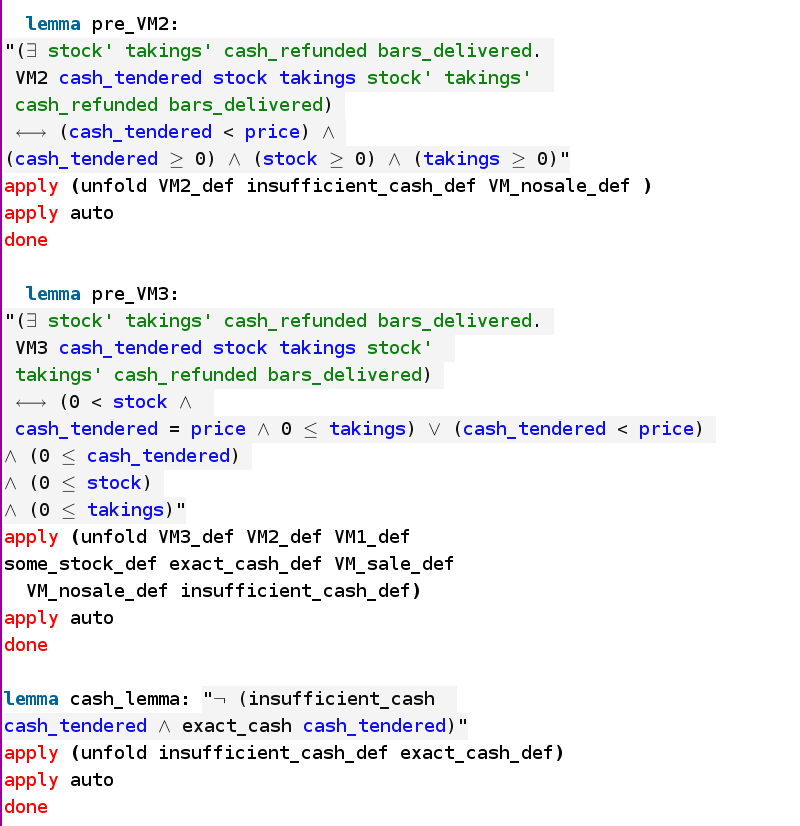
\includegraphics[scale=0.5]{examples/vm/6imaged.png}

\noindent 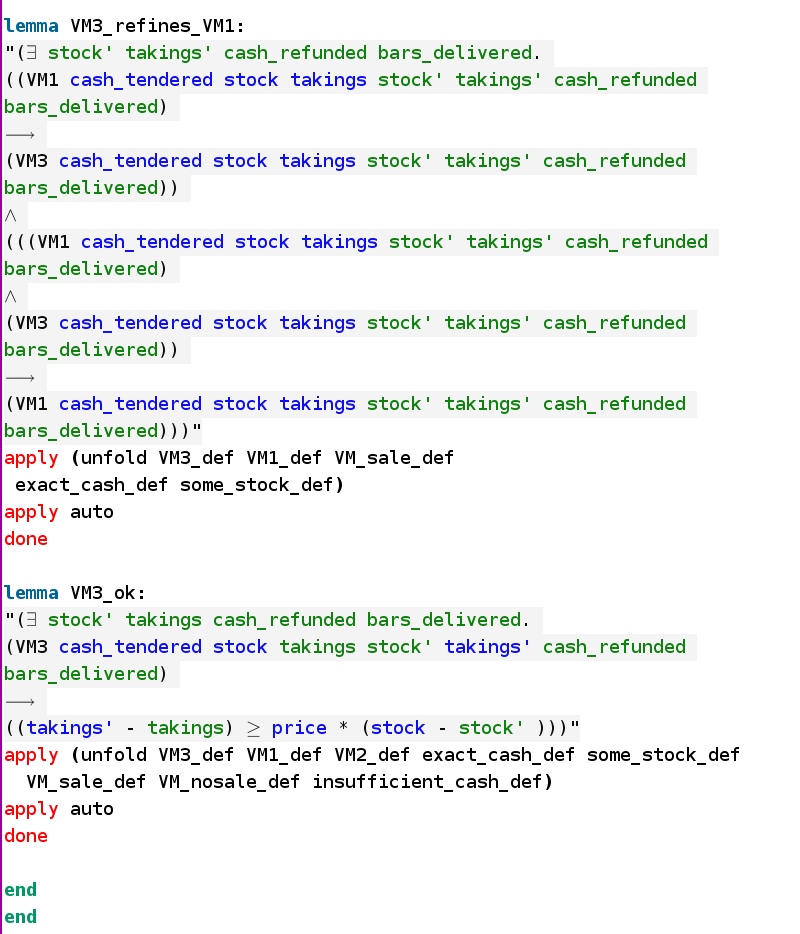
\includegraphics[scale=0.5]{examples/vm/6imagee.png}
%\input{examples/vm/6.thy}

\section{BirthdayBook}
\label{app:bb}

\subsection{Raw Latex}
\label{app:bb0}
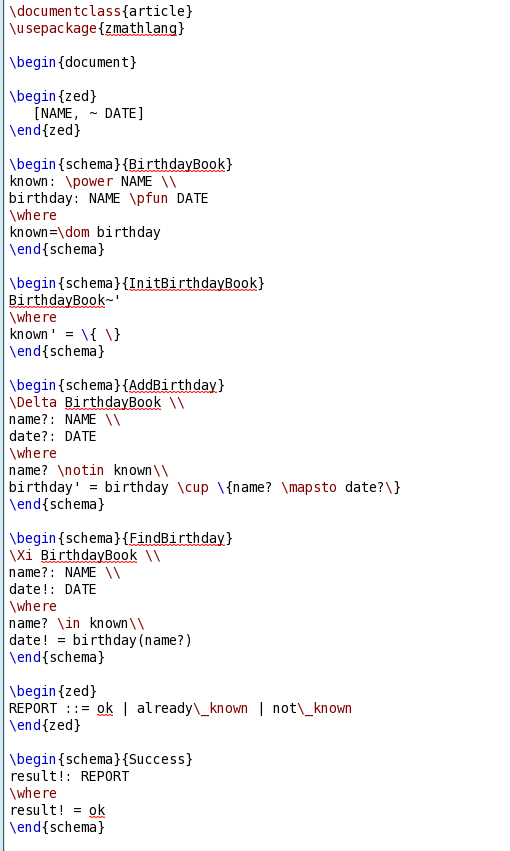
\includegraphics[scale=0.5]{examples/bb/0imagea.png}

\noindent 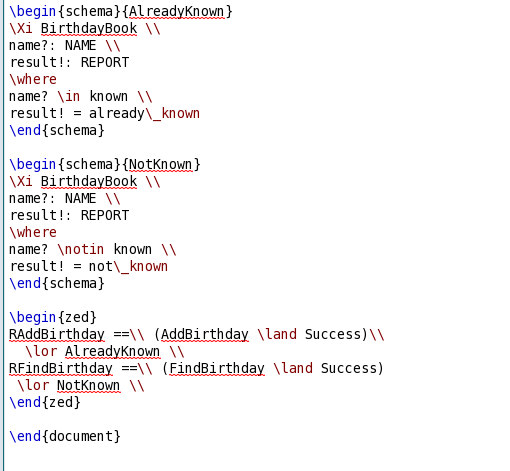
\includegraphics[scale=0.5]{examples/bb/0imageb.png}
%\begin{verbatim}
\documentclass{article}
\usepackage{zmathlang}

\begin{document}

\begin{zed}
   [NAME, ~ DATE] 
\end{zed}

\begin{schema}{BirthdayBook}
known: \power NAME \\ 
birthday: NAME \pfun DATE 
\where 
	known=\dom birthday
\end{schema}

\begin{schema}{InitBirthdayBook} 
BirthdayBook~' 
\where 
	known' = \{ \}
\end{schema}

\begin{schema}{AddBirthday}
    \Delta BirthdayBook \\
    name?: NAME \\
    date?: DATE
\where
    name? \notin known\\
    birthday' = birthday \cup \{name? \mapsto date?\}
\end{schema}

\begin{schema}{FindBirthday}
    \Xi BirthdayBook \\
    name?: NAME \\
    date!: DATE 
\where
    	name? \in known\\
    	date! = birthday(name?)
\end{schema}

\begin{zed} 
    REPORT ::= ok | already\_known | not\_known
\end{zed}

\begin{schema}{Success}
    result!: REPORT
\where
    result! = ok
\end{schema}

\begin{schema}{AlreadyKnown}
    \Xi BirthdayBook \\
    name?: NAME \\
    result!: REPORT
\where
	name? \in known \\
	result! = already\_known
\end{schema}

\begin{schema}{NotKnown}
    \Xi BirthdayBook \\
    name?: NAME \\
    result!: REPORT
\where
	name? \notin known \\
	result! = not\_known
\end{schema}

\begin{zed} 
    RAddBirthday ==\\ (AddBirthday \land Success)\\
      \lor AlreadyKnown \\
    RFindBirthday ==\\ (FindBirthday \land Success)
     \lor NotKnown \\
\end{zed}

\end{document}
\end{verbatim}
\subsection{Raw Latex output}
\label{app:bb0o}

\noindent 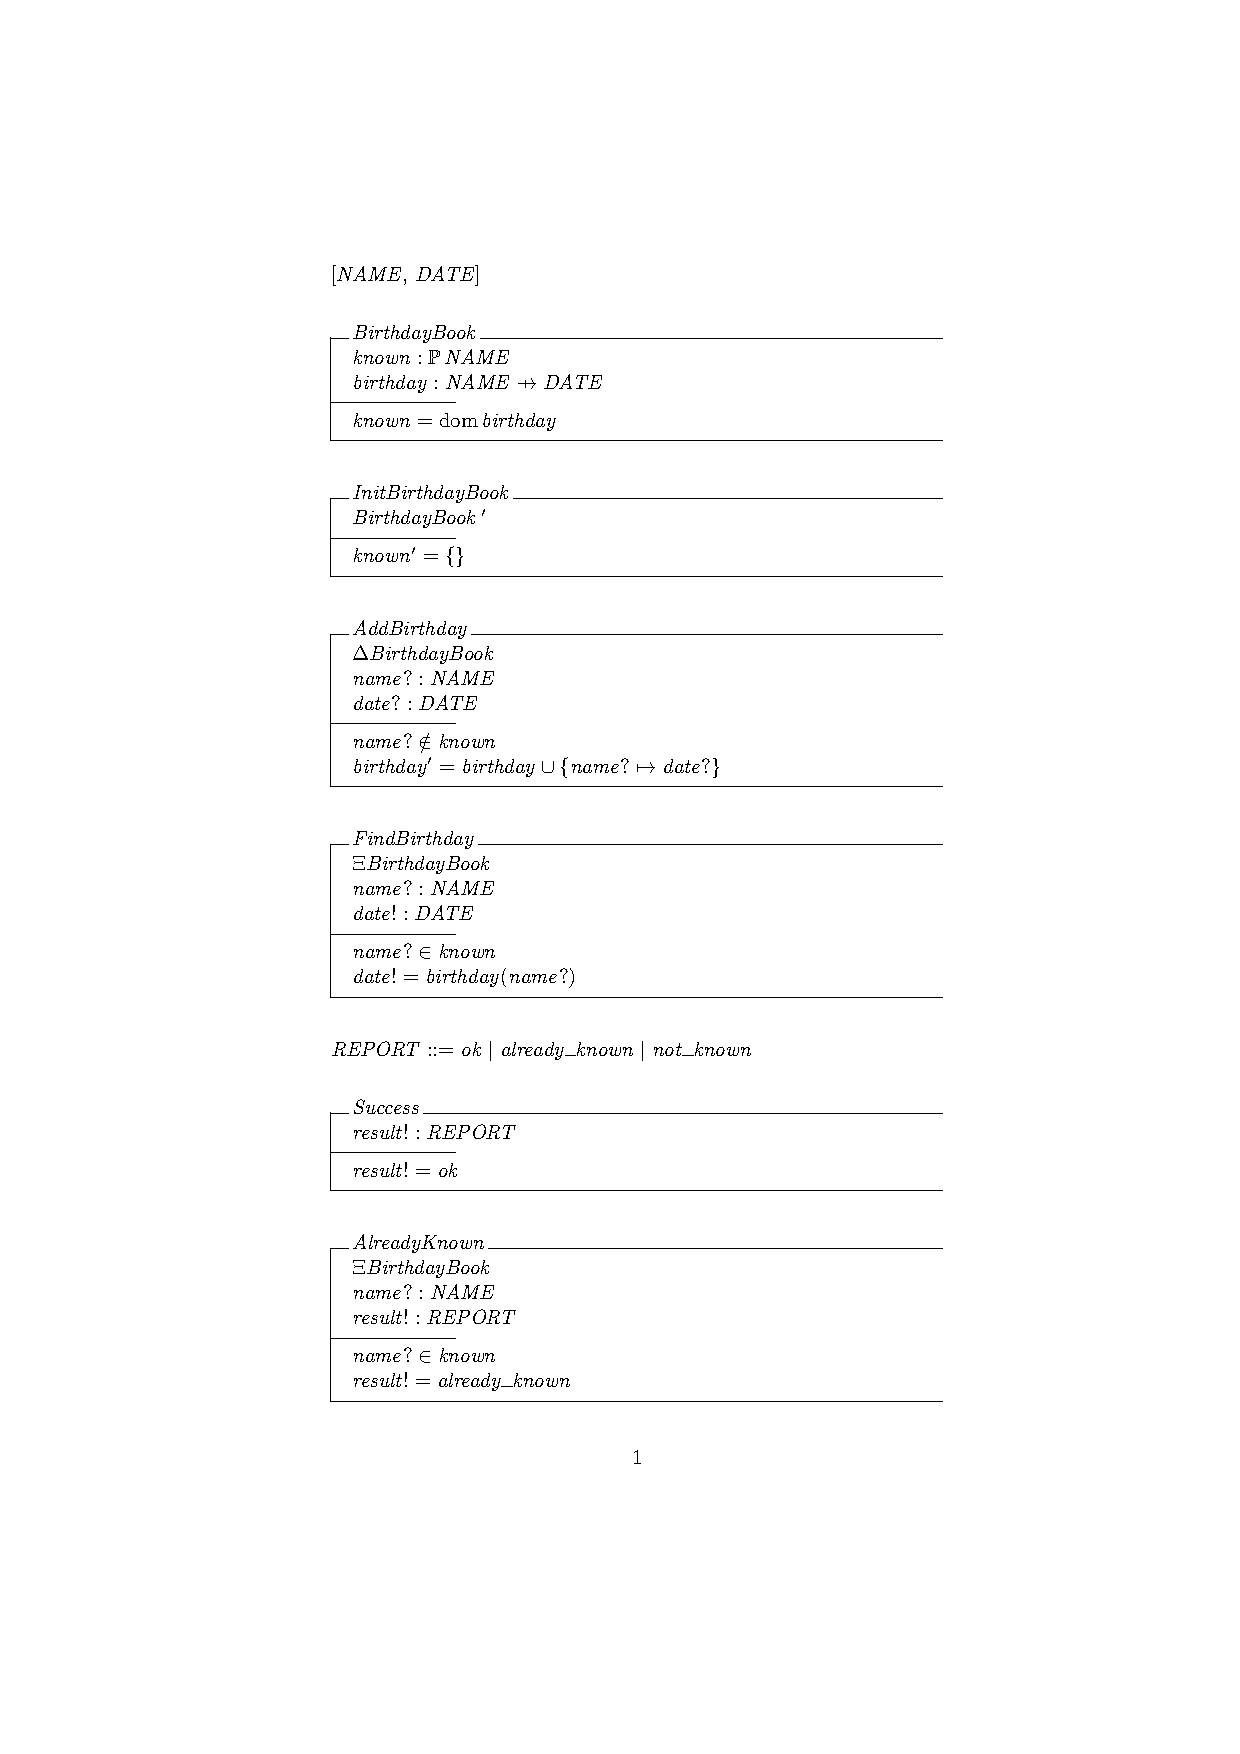
\includegraphics[clip, trim=4cm 5.5cm 4cm 4.2cm]{examples/bb/0comp.pdf}

\noindent 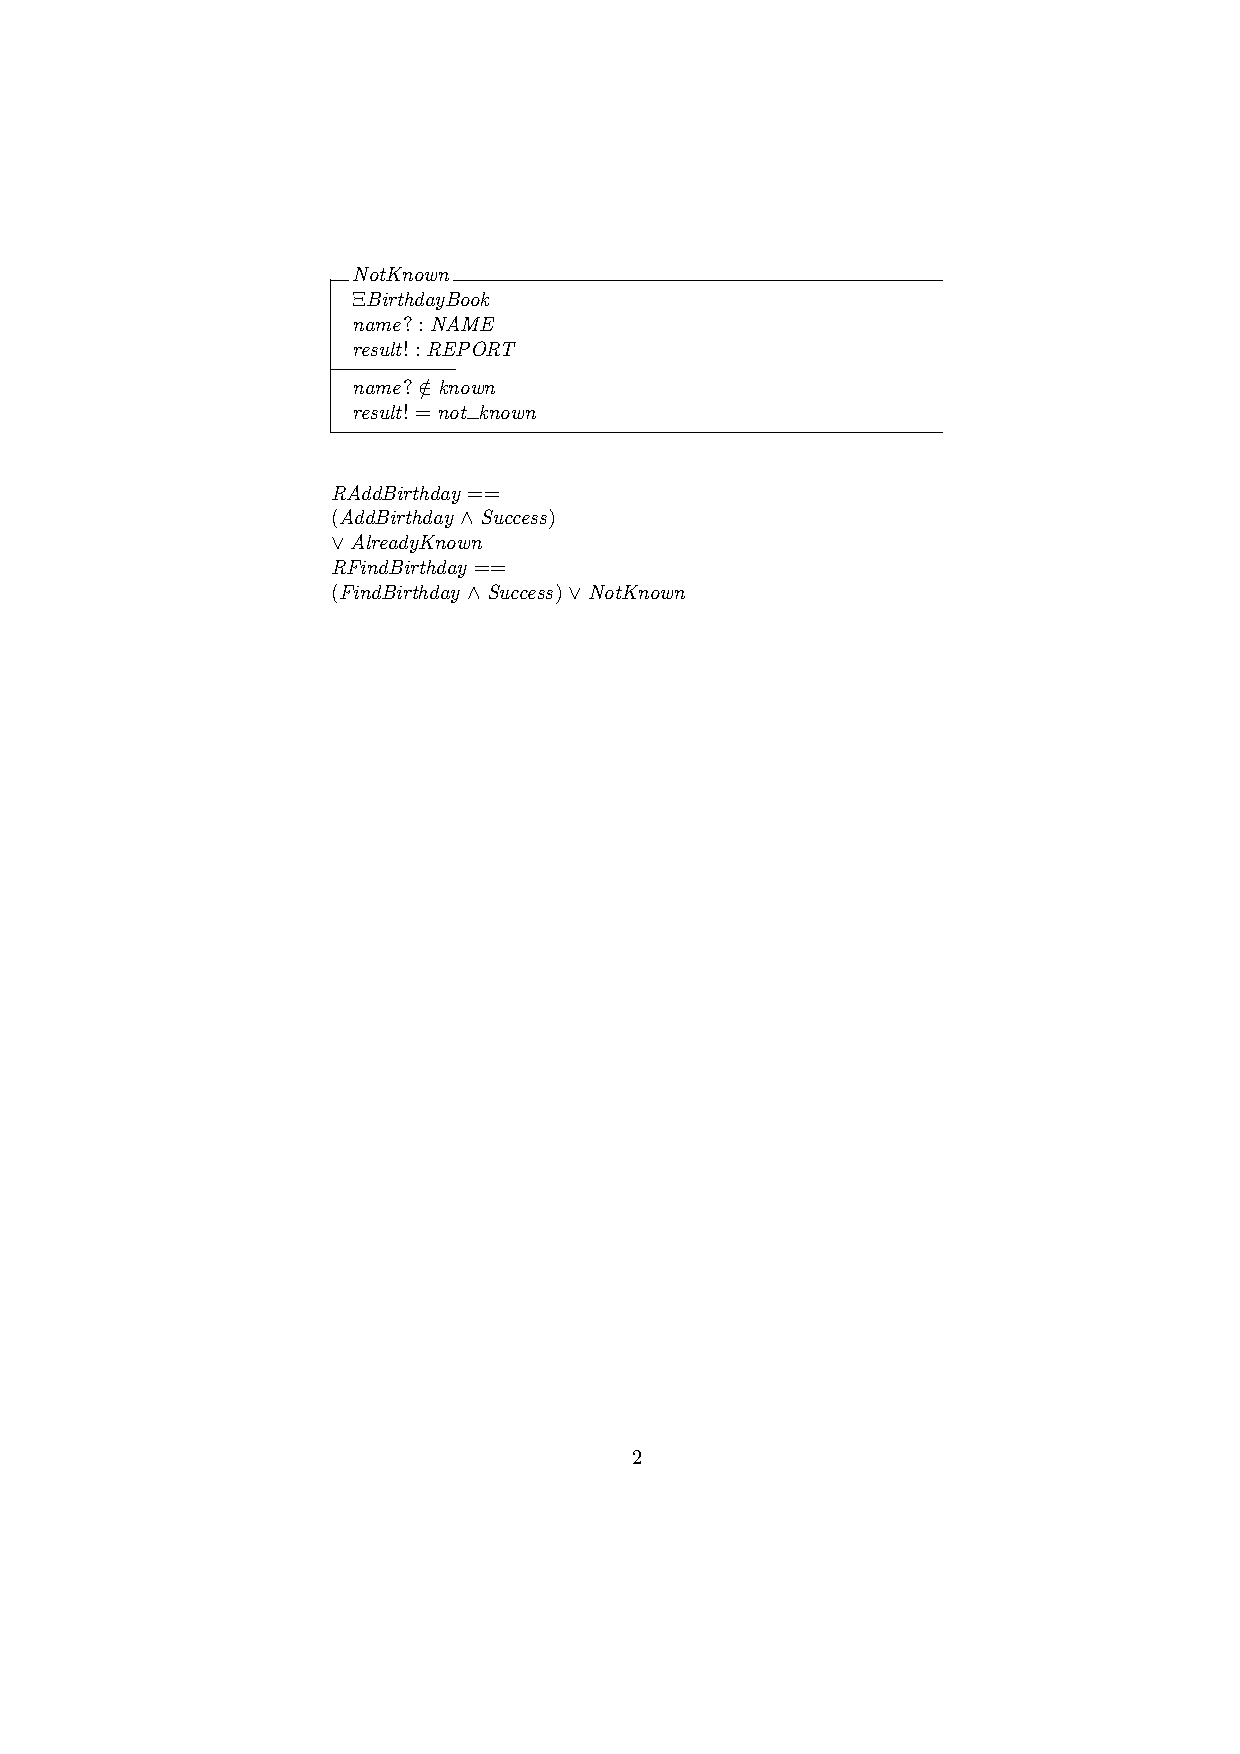
\includegraphics[clip, trim=4cm 10cm 4cm 4.2cm]{examples/bb/0comp2.pdf}

%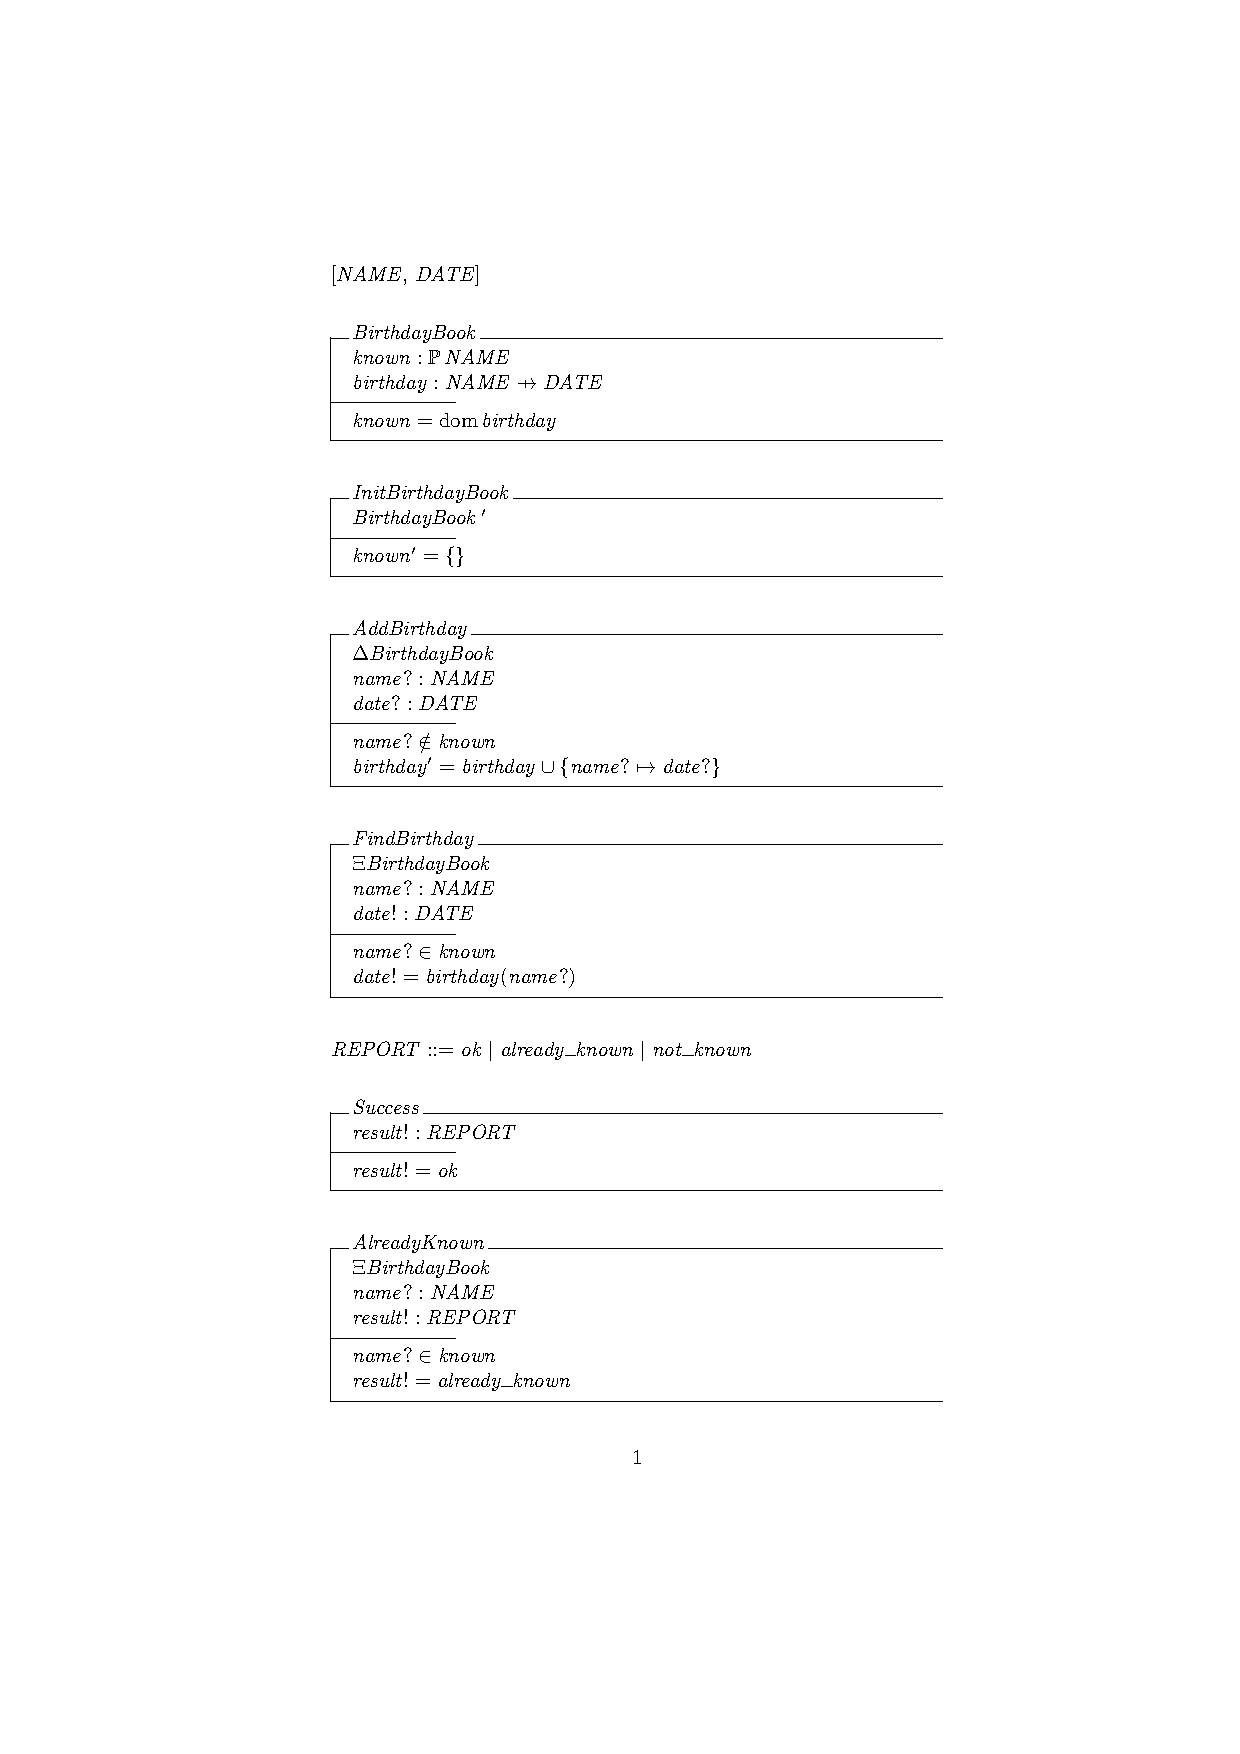
\includepdf[pages={1-2}]{examples/bb/0comp.pdf}
\subsection{ZCGa Annotated Latex Code}
\label{app:bb1}

\begin{figure}[H]
    \hfill
    \subfigure{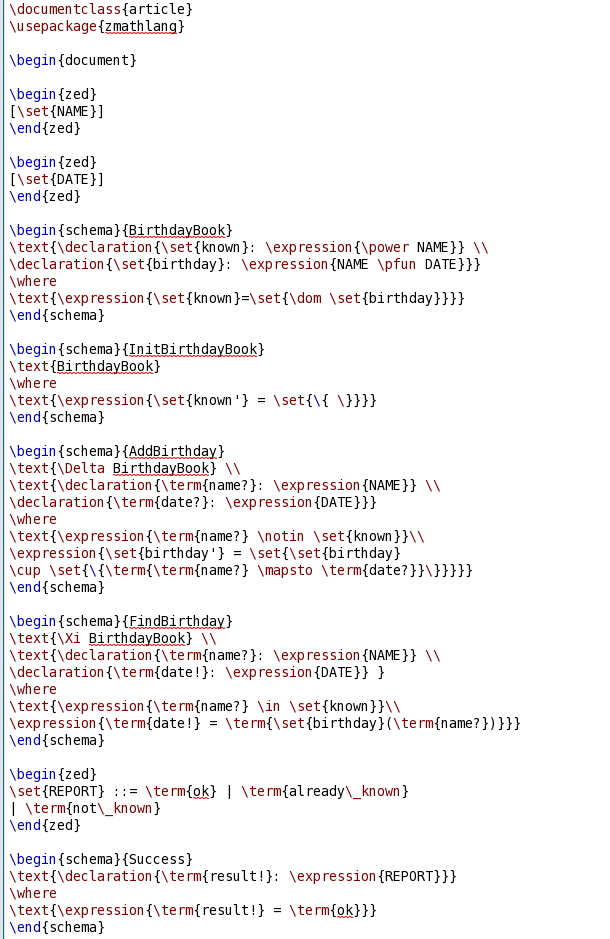
\includegraphics[width=9cm]{examples/bb/1imagea.png}}
    \hfill
    \subfigure{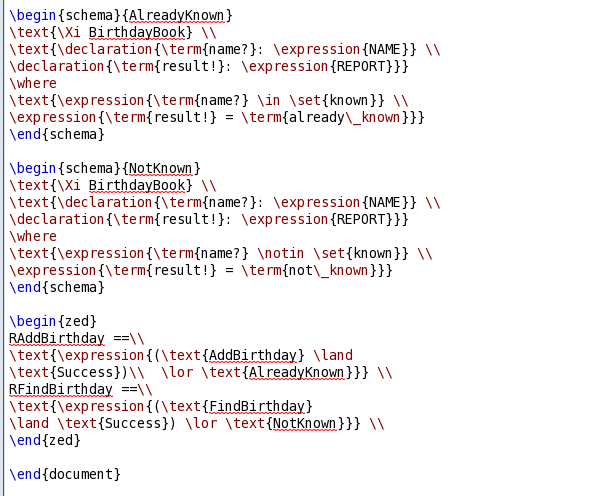
\includegraphics[width=9cm]{examples/bb/1imageb.png}}
    \hfill
\end{figure}
%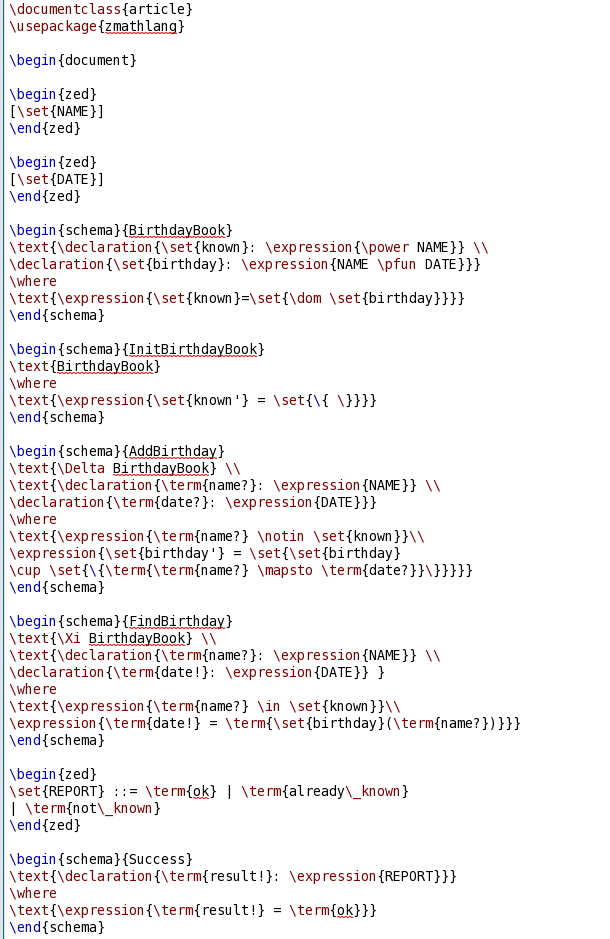
\includegraphics[scale=0.5]{examples/bb/1imagea.png}

%\noindent 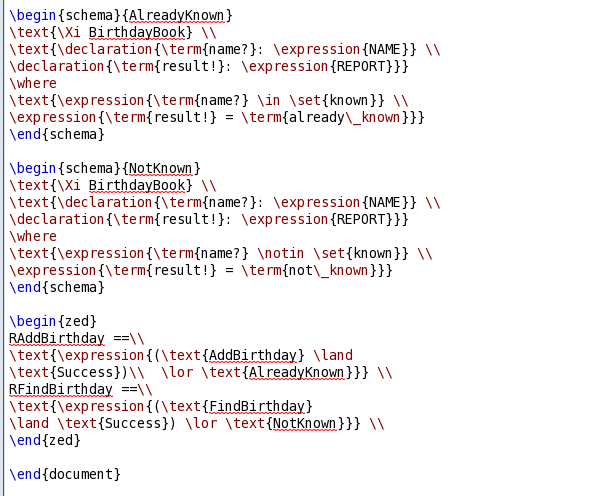
\includegraphics[scale=0.5]{examples/bb/1imageb.png}

\subsection{ZCGa output}
\label{app:bb1o}
\noindent 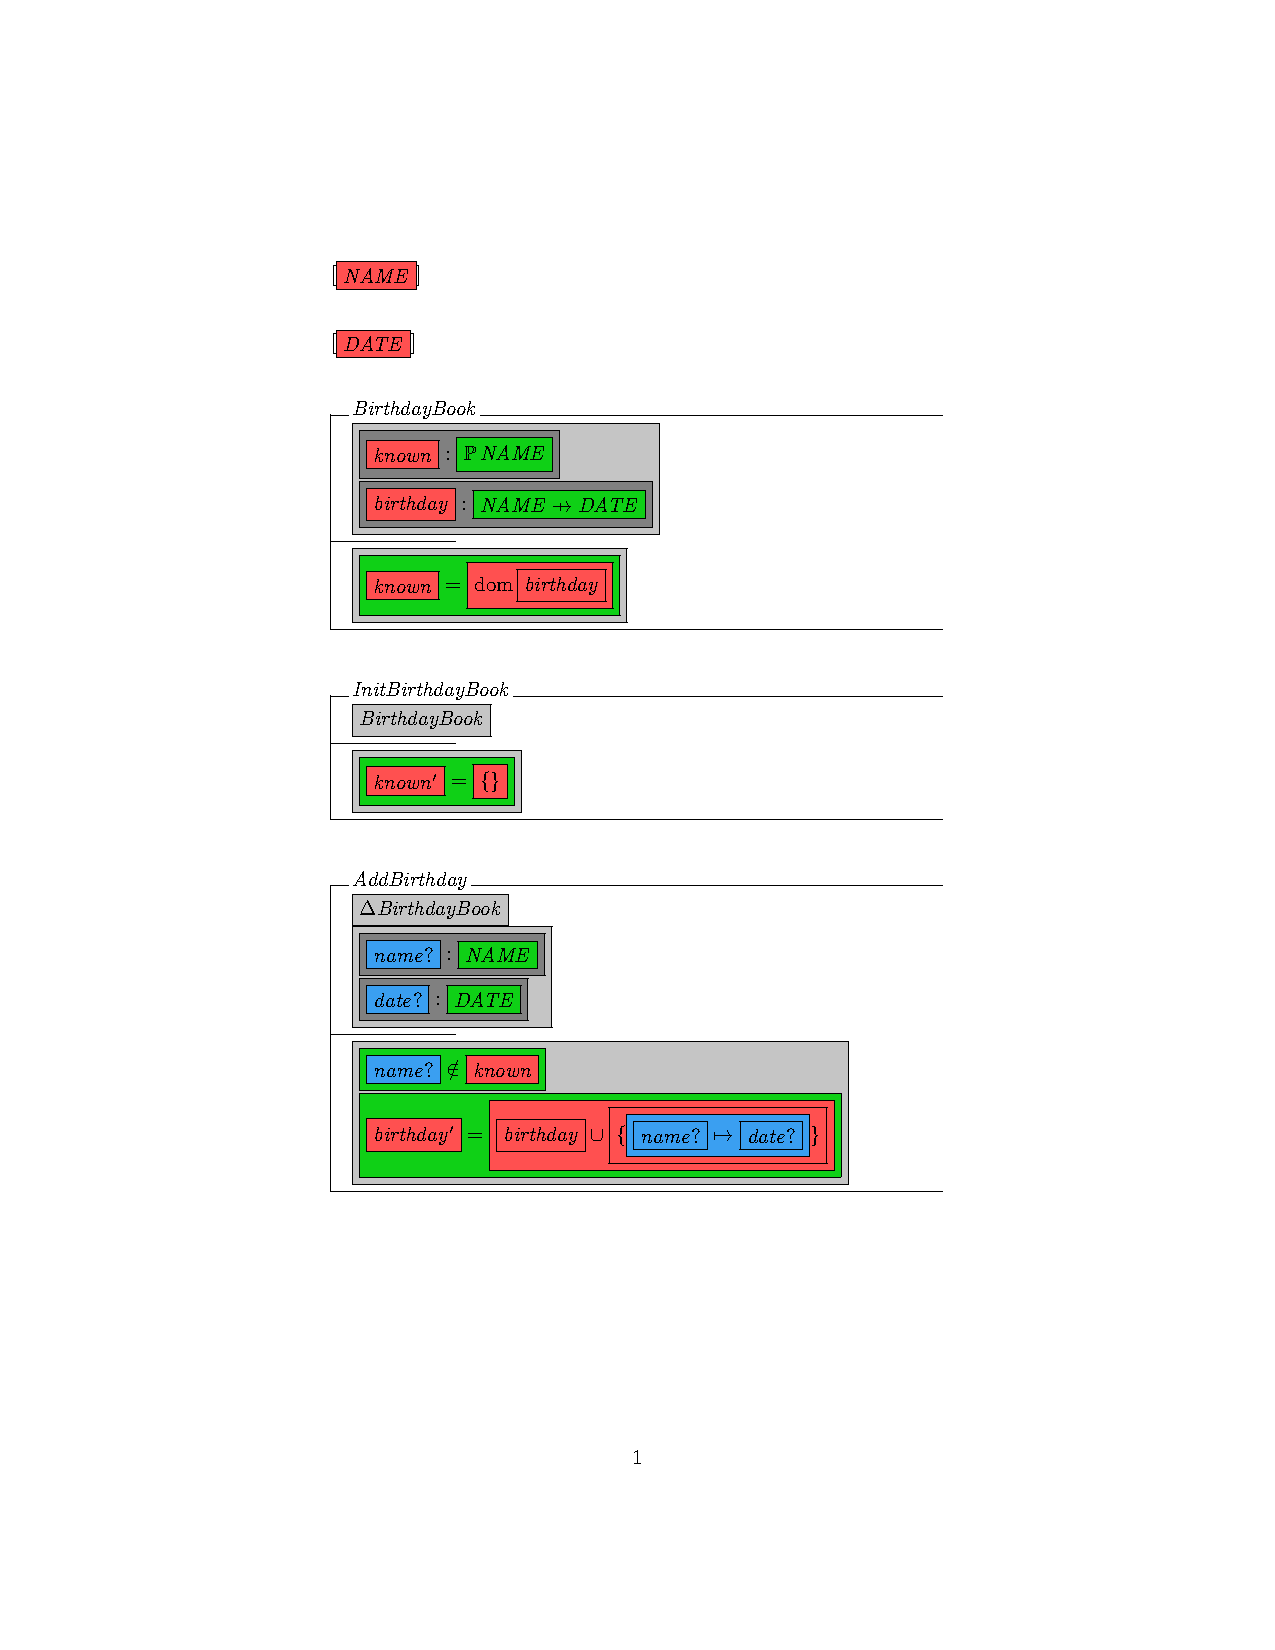
\includegraphics[clip, trim=4cm 6cm 4cm 4.2cm]{examples/bb/1comp.pdf}

\noindent 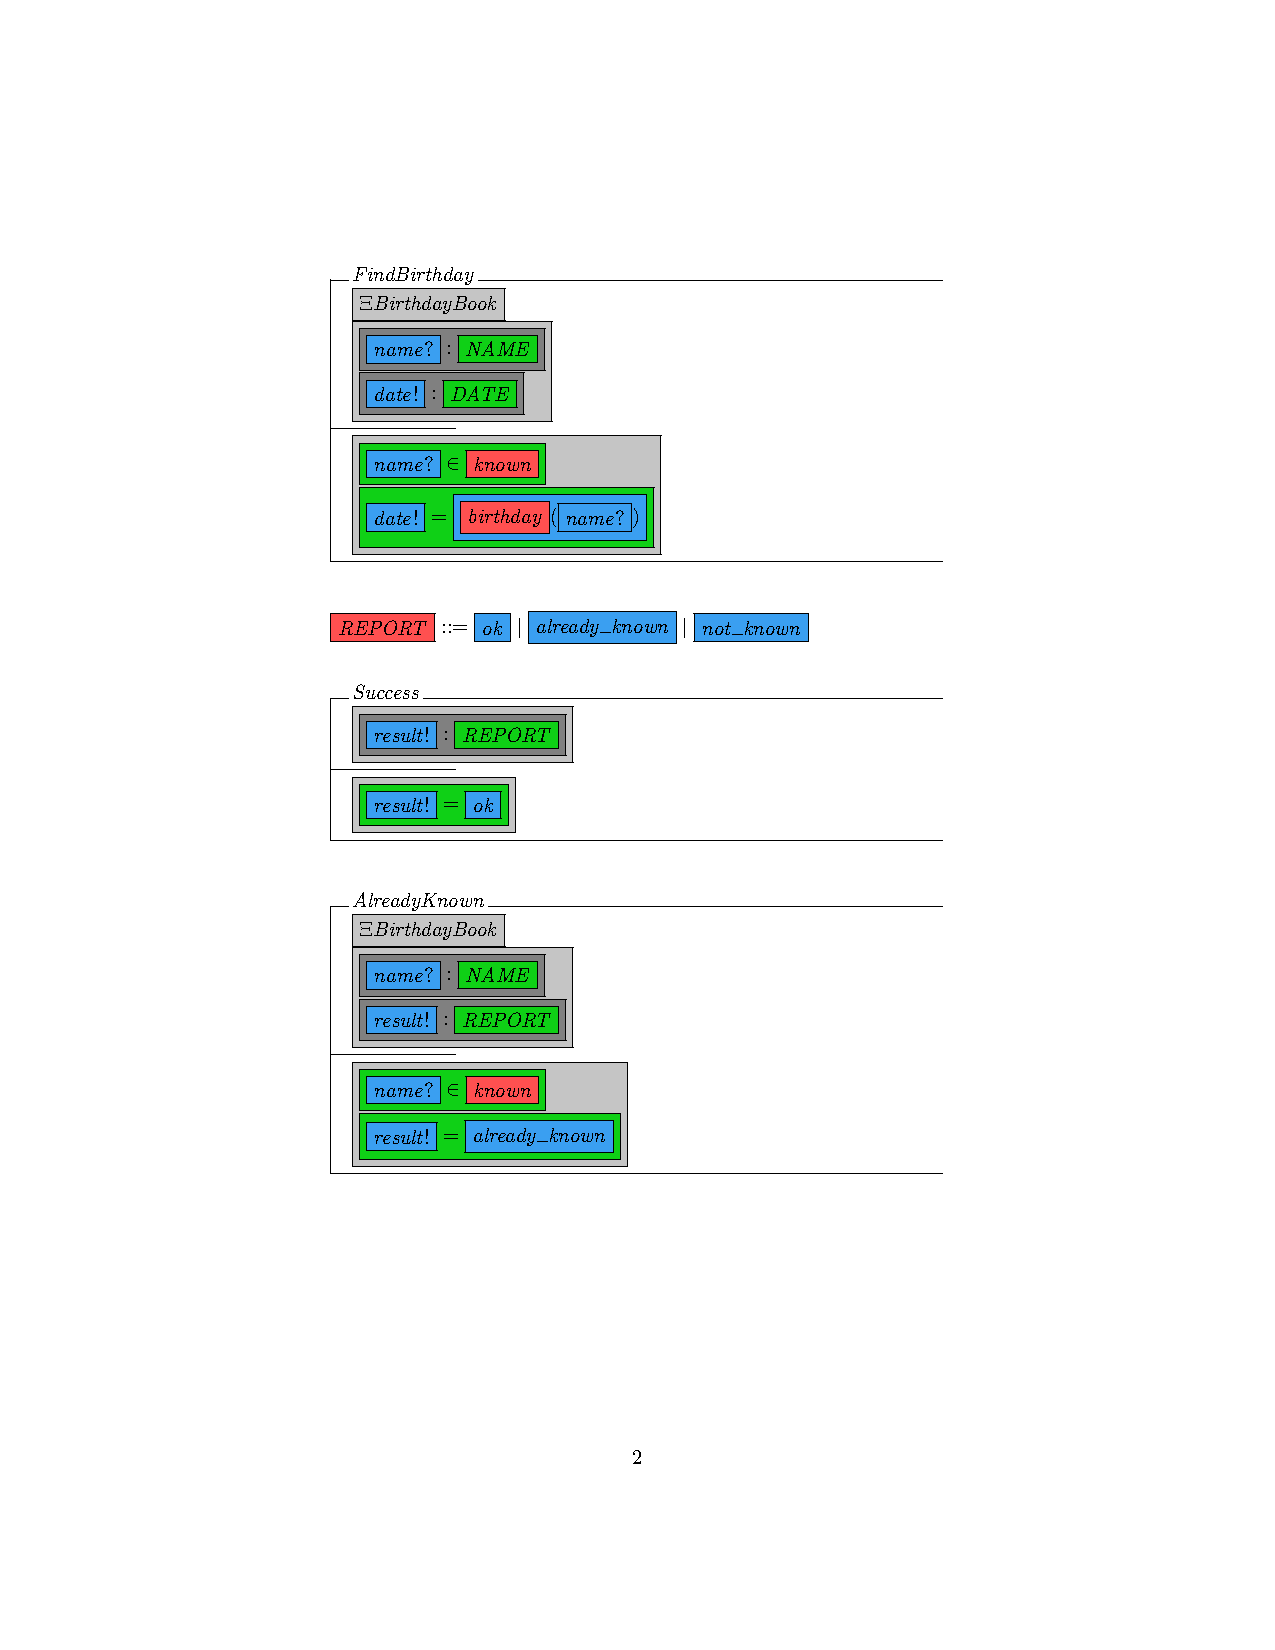
\includegraphics[clip, trim=4cm 8cm 4cm 4.2cm]{examples/bb/1comp2.pdf}

\noindent 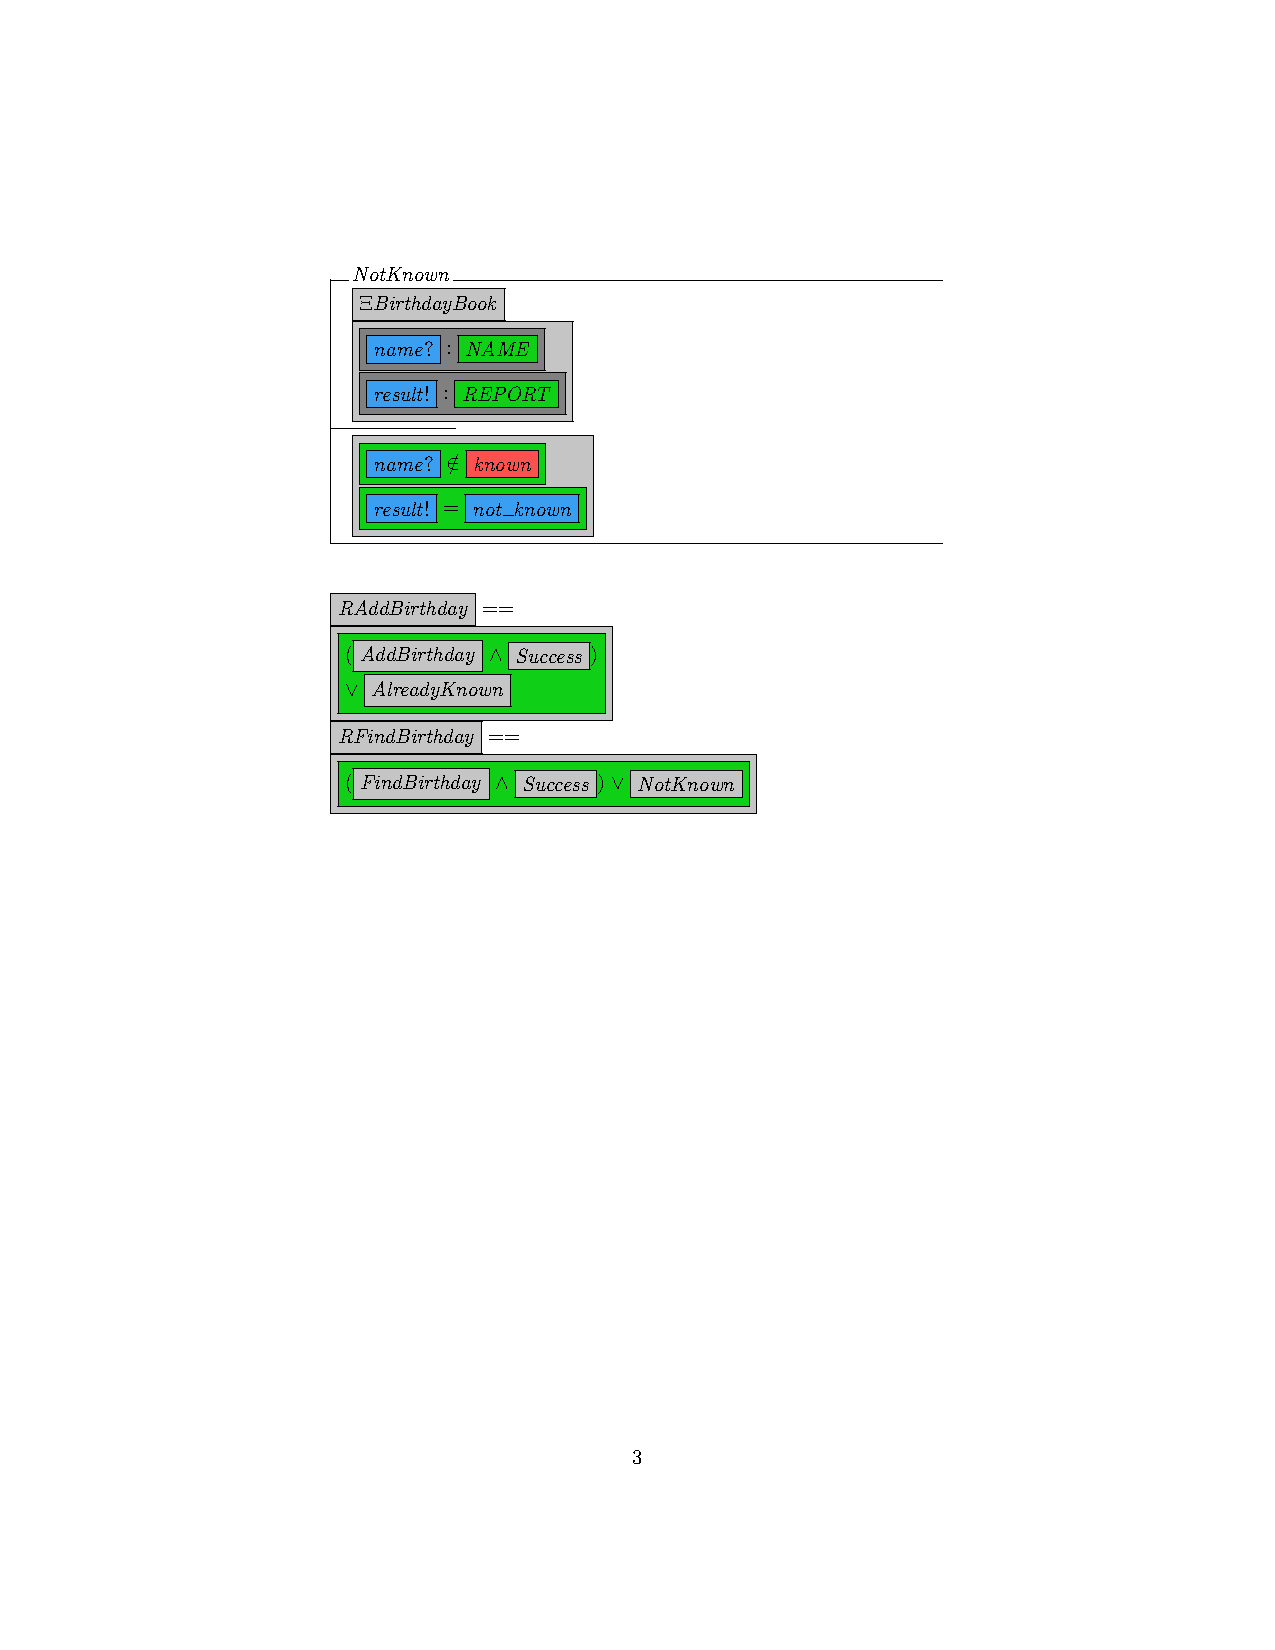
\includegraphics[clip, trim=4cm 8cm 4cm 4.2cm]{examples/bb/1comp3.pdf}

\subsection{ZDRa Annotated Latex Code}
\label{app:bb2}
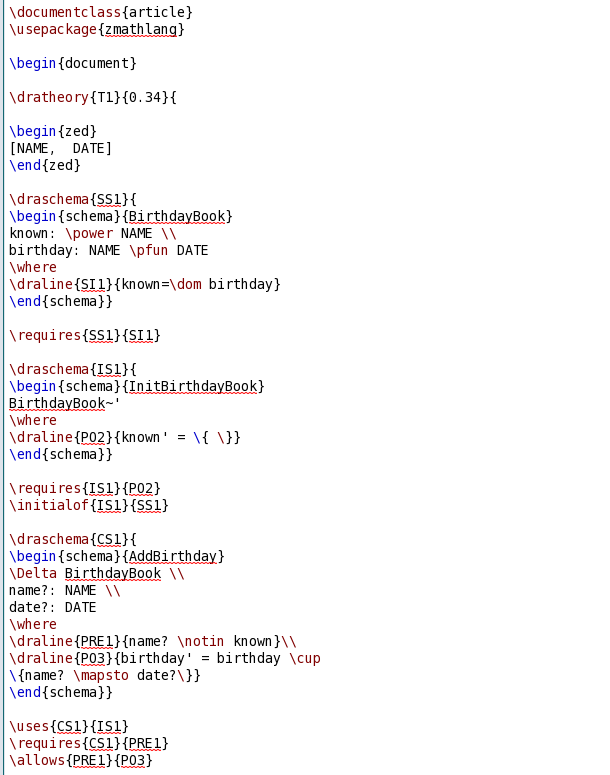
\includegraphics[scale=0.5]{examples/bb/2imagea.png}

\noindent 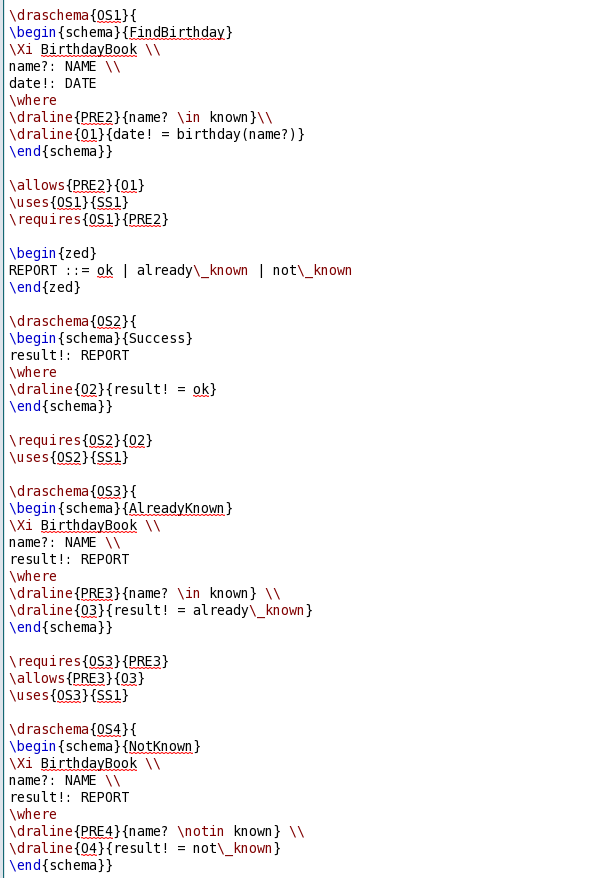
\includegraphics[scale=0.5]{examples/bb/2imageb.png}

\noindent \includegraphics[scale=0.5]{examples/bb/2imagec.png}
%\begin{verbatim}
\documentclass{article}
\usepackage{zmathlang}

\begin{document}

\dratheory{T1}{0.34}{

\begin{zed}
   [NAME, ~ DATE] 
\end{zed}

\draschema{SS1}{
\begin{schema}{BirthdayBook}
known: \power NAME \\ 
birthday: NAME \pfun DATE 
\where 
\draline{SI1}{known=\dom birthday}
\end{schema}}

\requires{SS1}{SI1}

\draschema{IS1}{
\begin{schema}{InitBirthdayBook} 
BirthdayBook~' 
\where 
\draline{PO2}{known' = \{ \}}
\end{schema}}

\requires{IS1}{PO2}
\initialof{IS1}{SS1}

\draschema{CS1}{
\begin{schema}{AddBirthday}
    \Delta BirthdayBook \\
    name?: NAME \\
    date?: DATE
\where
    \draline{PRE1}{name? \notin known}\\
    \draline{PO3}{birthday' = birthday \cup 
    \{name? \mapsto date?\}}
\end{schema}}

\uses{CS1}{IS1}
\requires{CS1}{PRE1}
\allows{PRE1}{PO3}

\draschema{OS1}{
\begin{schema}{FindBirthday}
    \Xi BirthdayBook \\
    name?: NAME \\
    date!: DATE 
\where
    \draline{PRE2}{name? \in known}\\
    \draline{O1}{date! = birthday(name?)}
\end{schema}}

\allows{PRE2}{O1}
\uses{OS1}{SS1}
\requires{OS1}{PRE2}

\begin{zed} 
    REPORT ::= ok | already\_known | not\_known
\end{zed}

\draschema{OS2}{
\begin{schema}{Success}
    result!: REPORT
\where
    \draline{O2}{result! = ok}
\end{schema}}

\requires{OS2}{O2}
\uses{OS2}{SS1}

\draschema{OS3}{
\begin{schema}{AlreadyKnown}
    \Xi BirthdayBook \\
    name?: NAME \\
    result!: REPORT
\where
    \draline{PRE3}{name? \in known} \\
    \draline{O3}{result! = already\_known}
\end{schema}}

\requires{OS3}{PRE3}
\allows{PRE3}{O3}
\uses{OS3}{SS1}

\draschema{OS4}{
\begin{schema}{NotKnown}
    \Xi BirthdayBook \\
    name?: NAME \\
    result!: REPORT
\where
    \draline{PRE4}{name? \notin known} \\
    \draline{O4}{result! = not\_known}
\end{schema}}

\requires{OS4}{PRE4}
\allows{PRE4}{O4}
\uses{OS4}{SS1}

\begin{zed} 
    \draline{TS1}{RAddBirthday == (AddBirthday \land Success)
      \lor AlreadyKnown} \\
   \draline{TS2}{RFindBirthday ==\\ (FindBirthday \land Success)
    \lor NotKnown} \\
\end{zed}

\totalises{TS1}{CS1}
\totalises{TS1}{OS2}
\totalises{TS1}{OS3}
\totalises{TS2}{OS1}
\totalises{TS2}{OS2}
\totalises{TS2}{OS4}
}

\end{document}
\end{verbatim}
\subsection{ZDRa Output}
\label{app:bb2o}

\noindent \includegraphics[clip, trim=0cm 4cm 6cm 4.2cm]{examples/bb/2comp.pdf}

%\includepdf[pages={1}]{examples/bb/2comp.pdf}
\subsection{ZCGa and ZDRa Annotated Latex Code}
\label{app:bb1n2}
\includegraphics[scale=0.5]{examples/bb/1n2imagea.png}

\noindent \includegraphics[scale=0.5]{examples/bb/1n2imageb.png}

\noindent \includegraphics[scale=0.5]{examples/bb/1n2imagec.png}
%\begin{verbatim}
\documentclass{article}
\usepackage{zmathlang}

\begin{document}

\dratheory{T1}{0.3}{

\begin{zed}
[\set{NAME}] 
\end{zed}

\begin{zed}
[\set{DATE}]
\end{zed}

\draschema{SS1}{
\begin{schema}{BirthdayBook}
    \text{\declaration{\set{known}:\expression{\power NAME}}} \\
    \text{\declaration{\set{birthday}:\expression{NAME \pfun DATE}}}
\where
    \draline{SI1}{\text{\expression{\set{known}=
    \set{\dom \set{birthday}}}}}
\end{schema}}

\requires{SS1}{SI1}

\draschema{IS1}{
\begin{schema}{InitBirthdayBook}
    \text{BirthdayBook}
\where
    \draline{PO2}{\text{\expression{\set{known'} = \set{\{ \}}}}}
\end{schema}}

\requires{IS1}{PO2}

\initialof{IS1}{SS1}

\draschema{CS1}{
\begin{schema}{AddBirthday}
    \text{\Delta BirthdayBook} \\
    \text{\declaration{\term{name?}: \expression{NAME}}} \\
    \text{\declaration{\term{date?}: \expression{DATE}}}
\where
    \draline{PRE1}{\text{\expression{\term{name?} \notin
     \set{known}}}}\\
    \draline{PO3}{\expression{\set{birthday'} = 
    \set{\set{birthday} \cup 
    \set{\{\term{\term{name?} \mapsto \term{date?}}\}}}}}
\end{schema}}

\uses{CS1}{IS1}
\requires{CS1}{PRE1}
\allows{PRE1}{PO3}

\draschema{OS1}{
\begin{schema}{FindBirthday}
    \text{\Xi BirthdayBook} \\
    \text{\declaration{\term{name?}: \expression{NAME}}} \\
    \text{\declaration{\term{date!}: \expression{DATE}}}
\where
    \draline{PRE2}{\text{\expression{\term{name?} \in 
    \set{known}}}}\\
    \draline{O1}{\text{\expression{\term{date!} = 
    \term{\set{birthday}~(\term{name?})}}}}
\end{schema}}

\allows{PRE2}{O1}
\uses{OS1}{SS1}
\requires{OS1}{PRE2}

\begin{zed} 
    \set{REPORT} ::= \term{ok} | \term{already\_known} |
     \term{not\_known}
\end{zed}

\draschema{OS3}{
\begin{schema}{Success}
    \text{\declaration{\term{result!}: \expression{REPORT}}}
\where
    \draline{O3}{\text{\expression{\term{result!} = \term{ok}}}}
\end{schema}}

\requires{OS3}{O3}
\uses{OS3}{SS1}

\draschema{OS4}{
\begin{schema}{AlreadyKnown}
    \text{\Xi BirthdayBook} \\
    \text{\declaration{\term{name?}: \expression{NAME}}} \\
    \text{\declaration{\term{result!}: \expression{REPORT}}}
\where
    \draline{PRE3}{\text{\expression{\term{name?} \in
    \set{known}}}} \\
    \draline{O4}{\text{\expression{\term{result!} =
    \term{already\_known}}}}
\end{schema}}

\requires{OS4}{PRE3}
\allows{PRE3}{O4}
\uses{OS4}{SS1}

\draschema{OS5}{
\begin{schema}{NotKnown}
    \text{\Xi BirthdayBook} \\
    \text{\declaration{\term{name?}:\expression{NAME}}} \\
    \text{\declaration{\term{result!}:\expression{REPORT}}}
\where
    \draline{PRE4}{\text{\expression{\term{name?} \notin
     \set{known}}}} \\
    \draline{O5}{\text{\expression{\term{result!} =
     \term{not\_known}}}}
\end{schema}}

\requires{OS5}{PRE4}
\allows{PRE4}{O5}
\uses{OS5}{SS1}

\begin{zed} 
    \draschema{TS1}{RAddBirthday == 
    \text{\expression{(\text{AddBirthday} \land 
    \text{Success})\\  \lor \text{AlreadyKnown}}}} \\
    \draschema{TS2}{RFindBirthday == 
    \text{\expression{(\text{FindBirthday} \land 
    \text{Success}) \lor \text{NotKnown}}}} 
\end{zed}

\totalises{TS1}{CS1}
\totalises{TS1}{OS3}
\totalises{TS1}{OS4}
\totalises{TS2}{OS1}
\totalises{TS2}{OS3}
\totalises{TS2}{OS5}

}
\end{document}
\end{verbatim}
\subsection{ZCGa and ZDRa output}
\label{app:bb1n2o}
\noindent \includegraphics[clip, trim=0cm 4cm 6cm 4.2cm]{examples/bb/1n2comp.pdf}

\subsection{Dependency and Goto Graphs}
\label{app:bb2.5}
\includegraphics[scale=0.7]{examples/bb/25a.png}

\includegraphics[scale=0.7]{examples/bb/25b.png}
\subsection{General Proof Skeleton}
\label{app:bb3}
\input{examples/bb/new3.txt}
\subsection{Isabelle Proof Skeleton}
\label{app:bb4}
\includegraphics[scale=0.5]{examples/bb/4imagea.png}

\noindent \includegraphics[scale=0.5]{examples/bb/4imageb.png}

\noindent \includegraphics[scale=0.5]{examples/bb/4imagec.png}
%\input{examples/bb/new4.thy}
\subsection{Isabelle Filled In}
\label{app:bb5}
\includegraphics[scale=0.4]{examples/bb/5imagea.png}

\noindent \includegraphics[scale=0.4]{examples/bb/5imageb.png}

\noindent \includegraphics[scale=0.4]{examples/bb/5imagec.png}
%\input{examples/bb/new4.thy}
%\input{examples/bb/new5.thy}
\subsection{Full Proof in Isabelle}
\label{app:bb6}
\includegraphics[scale=0.4]{examples/bb/6imagea.png}

\noindent \includegraphics[scale=0.4]{examples/bb/6imageb.png}

\noindent \includegraphics[scale=0.4]{examples/bb/6imagec.png}

\noindent \includegraphics[scale=0.4]{examples/bb/6imaged.png}

\noindent \includegraphics[scale=0.4]{examples/bb/6imagee.png}
%\begin{scriptsize}
\begin{verbatim}
theory modulereg
imports 
Main 
begin 
typedecl PERSON 
typedecl MODULE
record ModuleReg = 
STUDENTS :: " PERSON set"
DEGMODULES :: " MODULE set"
TAKING :: "(PERSON * MODULE) set"
locale Themodulereg = 
fixes students :: " PERSON set"
and degModules :: " MODULE set"
and taking :: "(PERSON * MODULE) set"
assumes "Domain taking \<subseteq> students" 
 and "Range taking \<subseteq> degModules"
begin
definition RegForModule :: 
"ModuleReg \<Rightarrow> ModuleReg \<Rightarrow> PERSON
\<Rightarrow> MODULE => MODULE set \<Rightarrow> PERSON set
\<Rightarrow> (PERSON * MODULE) set \<Rightarrow> bool"
where 
"RegForModule modulereg modulereg' p m degModules'
students' taking' ==
(p \<in> students) 
\<and> (m \<in> degModules) 
\<and> ((p, m) \<notin> taking)
\<and> (taking' = taking \<union> {(p, m)}) 
\<and> (students' = students) 
\<and> (degModules' = degModules)"

definition AddStudent :: 
"ModuleReg \<Rightarrow> ModuleReg => PERSON \<Rightarrow>
MODULE set \<Rightarrow> PERSON set \<Rightarrow>
(PERSON * MODULE) set \<Rightarrow> bool"
where 
"AddStudent modulereg modulereg' p degModules'
students' taking' ==
((p \<notin> students)
\<and> (students' = students \<union> {(p)}) 
\<and> (degModules' = degModules) 
\<and> (taking' = taking))"

(*The proof obligations generated by ZMathLang start here*)

lemma RegForModule_L1:
"(\<exists> degModules:: MODULE set.
\<exists> students :: PERSON set.
\<exists> taking :: (PERSON * MODULE) set.
\<exists> p :: PERSON.
\<exists> degModules':: MODULE set.
\<exists> students' :: PERSON set.
\<exists> taking' :: (PERSON * MODULE) set.
\<exists> m :: MODULE.
((p \<in> students) 
\<and> (m \<in> degModules) 
\<and> ((p, m) \<notin> taking)
\<and> (taking' = taking \<union> {(p, m)}) 
\<and> (students' = students) 
\<and> (degModules' = degModules))
\<and> (Domain taking \<subseteq> students)
\<and> (Range taking \<subseteq> degModules)
\<and> (Domain taking' \<subseteq> students')
\<and> (Range taking' \<subseteq> degModules'))"
by (smt Domain_empty Domain_insert Range.intros Range_empty 
Range_insert Un_empty Un_insert_right empty_iff empty_subsetI 
empty_subsetI insert_mono insert_mono singletonI singletonI 
singleton_insert_inj_eq' singleton_insert_inj_eq')

lemma AddStudent_L2:
"(\<exists> degModules:: MODULE set.
\<exists> students :: PERSON set.
\<exists> taking :: (PERSON * MODULE) set.
\<exists> p :: PERSON.
\<exists> degModules':: MODULE set.
\<exists> students' :: PERSON set.
\<exists> taking' :: (PERSON * MODULE) set.
 ((students' = students \<union> {(p)}) 
\<and> (degModules' = degModules) 
\<and> (taking' = taking))
\<and> (Domain taking \<subseteq> students)
\<and> (Range taking \<subseteq> degModules)
\<and> (Domain taking' \<subseteq> students')
\<and> (Range taking' \<subseteq> degModules'))"
by blast

(*Here I add other safety properties about the ModuleReg specification 
which I wish to prove*)

lemma pre_AddStudent:
"(\<exists> modulereg modulereg' students' degModules' taking'.
AddStudent modulereg modulereg' p degModules' students' taking')
\<longleftrightarrow> (p \<notin> students)"
apply (unfold AddStudent_def)
apply auto
done

lemma pre_RegForModule:
"(\<exists> modulereg modulereg' students' degModules' taking'.
RegForModule modulereg modulereg' p m degModules' students' taking')
 \<longleftrightarrow> (p \<in> students)
 \<and> (m \<in> degModules)
 \<and> ((p,m) \<notin> taking)"
 apply (unfold RegForModule_def)
 apply auto
done

definition InitModuleReg::
"ModuleReg \<Rightarrow> PERSON set \<Rightarrow
MODULE set \<Rightarrow> (PERSON * MODULE) set \<Rightarrow> bool"
where
"InitModuleReg modulereg' students' degmodules' taking' == ((
(students' = {})
\<and> (degmodules' = {})
\<and> (taking' = {})))"

lemma InitOK:
"(\<exists> modulereg'. InitModuleReg modulereg' 
tudents' degmodules' taking')
\<longrightarrow>  ((
(students' = {})
\<and> (degmodules' = {})
\<and> (taking' = {})))
\<and> ((Domain taking' \<subseteq> students')
\<and> (Range taking' \<subseteq> degModules'))"
by (simp add: InitModuleReg_def)

lemma RegForModuleNotEmpty:
"(\<exists> modulereg modulereg' students' degModules' taking' p m.
RegForModule modulereg modulereg' students' degModules' taking' p m)
 \<longrightarrow> (students \<noteq> {})
 \<and> (degModules \<noteq> {})"
by (smt RegForModule_def empty_iff empty_iff)

lemma notEmpty:
"(taking' = taking \<union> {(p,m)}) \<longrightarrow>
(taking' \<noteq> {})"
by (smt Un_empty insert_not_empty)

end
end
\end{verbatim}
\end{scriptsize}

\section{An example of a specification which fails \gls{zcga} but passes \gls{zdra}}
\label{app:nonworkingzcga}
This section shows an example of a specification which is rhetorically correct and passes the \gls{zdra} check however the grammar of the specification is incorrect and therefore fails the \gls{zcga} check. We input the compiled output for each of the examples. For reference to the code the reader is directed to \cite{mathlangexamples}.

\subsection{Raw Latex}
\includegraphics[scale=0.5]{examples/nonworkzcga/0imagea.png}

\noindent \includegraphics[scale=0.5]{examples/nonworkzcga/0imageb.png}

\noindent \includegraphics[scale=0.5]{examples/nonworkzcga/0imagec.png}

\noindent \includegraphics[scale=0.5]{examples/nonworkzcga/0imaged.png}

\noindent \includegraphics[scale=0.5]{examples/nonworkzcga/0imagee.png}

%\begin{verbatim}
\documentclass{article}
\usepackage{zmathlang}

\begin{document}

\begin{zed}
[NAME] 
\end{zed}

\begin{zed}
[SURNAME]
\end{zed}

\begin{zed}
[TELEPHONE]
\end{zed}

\begin{schema}{TelephoneDirectory}
persons: NAME \fun SURNAME \\ 
phoneNumbers: NAME \pfun TELEPHONE
\where 
\dom phoneNumbers=\dom persons
\end{schema}

\begin{schema}{InitTelephoneDirectory} 
TelephoneDirectory' 
\where 
phoneNumbers' = \{\}
persons' = \{\}
\end{schema}

\begin{schema}{AddPerson}
TheTelephoneDirectory \\
name?: NAME \\
surname?: SURNAME
phone?: TELEPHONE
\where
name? \mapsto surname? \notin persons\\
phoneNumbers' = phoneNumbers \cup \{name? \mapsto phone?\}
\end{schema}

\begin{schema}{AddNumber}
\Delta TelephoneDirectory \\
n?: NAME \\
s?: SURNAME
p?: TELEPHONE
\where
n \mapsto s \in persons\\
p? \notin \ran phoneNumbers \\
phoneNumbers' = phoneNumbers \cup \{n \mapsto phone?\}
\end{schema}

\begin{schema}{RemovePerson}
\Delta TelephoneDirectory \\
n?: NAME \\
s?: SURNAME
p?: TELEPHONE
\where
n? \mapsto s? \in persons\\
n? \mapsto p? \notin phoneNumbers \\
persons' = persons \setminus \{n? \mapsto s?\}
\end{schema}

\begin{zed}
OUTPUT ::= success | alreadyInDirectory | notInDirectory |numberInUse
\end{zed}

\begin{schema}{Success}
message!:OUTPUT
\where
message! = success
\end{schema}

\begin{schema}{AlreadyInDirectory}
message!:OUTPUT \\
n?: NAME \\
s?: SURNAME
\where
n? \mapsto s \in persons \\
message! = alreadyInDirectory
\end{schema}

\begin{schema}{NameNotInDirectory}
message!:OUTPUT \\
n?: NAME \\
s?: SURNAME
\where
n? \mapsto s? \notin persons \\
message! = NamenotInDirectory
\end{schema}

\begin{schema}{NumberInUse}
message!:OUTPUT \\
p?: TELEPHONE
\where
p? \in \ran phoneNumbers \\
message! = numberInUse
\end{schema}

\begin{zed}
TotalAddPerson \defs (AddPerson \land Success) \lor AlreadyInDirectory \\
TotalRemovePerson \defs (RemovePerson \land Success) \lor NameNotInDirectory \\
TotalAddNumber \defs (AddNumber \land Success) \lor NameNotInDirectory \lor NumberInUse \\
\end{zed}

\end{document}
\end{verbatim}
\subsection{Raw Latex output}

\noindent \includegraphics[clip, trim=4cm 8cm 4cm 4.2cm]{examples/nonworkzcga/0.pdf}

\noindent \includegraphics[clip, trim=4cm 8cm 3cm 4.2cm]{examples/nonworkzcga/0comp2.pdf}

%\includepdf[pages={1-2}]{examples/nonworkzcga/0.pdf}
\subsection{ZCGa and ZDRa Annotated Latex Code}
\label{app:nonzcga1n2}
\includegraphics[scale=0.5]{examples/nonworkzcga/1n2imagea.png}

\noindent \includegraphics[scale=0.5]{examples/nonworkzcga/1n2imageb.png}

\noindent \includegraphics[scale=0.5]{examples/nonworkzcga/1n2imagec.png}

\noindent \includegraphics[scale=0.5]{examples/nonworkzcga/1n2imaged.png}

\noindent \includegraphics[scale=0.5]{examples/nonworkzcga/1n2imagee.png}

\noindent \includegraphics[scale=0.5]{examples/nonworkzcga/1n2imagef.png}

\noindent \includegraphics[scale=0.5]{examples/nonworkzcga/1n2imageg.png}

\subsection{ZCGa and ZDRa output}
\noindent \includegraphics[clip, trim=0cm 4cm 6cm 4.2cm]{examples/nonworkzcga/1n2.pdf}

\subsection{Messages when running the specification through the ZCGa and ZDRa checks}

\begin{figure}[H]
\includegraphics[scale=0.7]{examples/nonworkzcga/incorrect.png}
\caption{Message when checking the specification for ZCGa correctness.}
\end{figure}

\begin{figure}[H]
\includegraphics[scale=0.7]{examples/nonworkzcga/correct.png}
\caption{Message when checking the specification for ZDRa correctness.}
\end{figure}

\section{An example of a specification which fails \gls{zdra} but passes \gls{zcga}}
\label{app:failzdra}
This section shows an example of a specification which is grammatically correct and passes the \gls{zcga} check however there are loops in it's rhetorical reasoning and therefore fails the \gls{zdra} check. We input the compiled output for each of the examples. For reference to the code the reader is directed to \cite{mathlangexamples}.

%\subsection{Raw Latex}
%\begin{verbatim}
\documentclass{article}
\usepackage{zmathlang}
\begin{document}

\begin{zed}
[NAME] 
\end{zed}

\begin{zed}
[SURNAME]
\end{zed}

\begin{zed}
[TELEPHONE]
\end{zed}

\begin{schema}{TelephoneDirectory}
persons: NAME \fun SURNAME \\ 
phoneNumbers: NAME \pfun TELEPHONE
\where 
\dom phoneNumbers = \dom persons
\end{schema}

\begin{schema}{InitTelephoneDirectory} 
TelephoneDirectory'
\where 
phoneNumbers' = \{\} \\
persons' = \{\}
\end{schema}

\begin{schema}{AddPerson}
\Delta TelephoneDirectory \\
name?: NAME \\
surname?: SURNAME \\
phone?: TELEPHONE
\where
name? \mapsto surname? \notin persons\\
persons' = persons \cup \{name? \mapsto surname?\}
\end{schema}

\begin{schema}{AddNumber}
\Delta TelephoneDirectory \\
n?: NAME \\
s?: SURNAME \\
p?: TELEPHONE
\where
n? \mapsto s? \in persons \\
p? \notin \ran phoneNumbers \\
phoneNumbers' = phoneNumbers \cup \{name? \mapsto phone?\}
\end{schema}

\begin{schema}{RemovePerson}
\Delta TelephoneDirectory \\
n?: NAME \\
s?: SURNAME \\
p?: TELEPHONE
\where
n? \mapsto s? \in persons\\
n? \mapsto p? \notin phoneNumbers \\
persons' = persons \setminus \{n? \mapsto s?\}
\end{schema}

\begin{schema}{RemoveNumber}
\Delta TelephoneDirectory \\
p?: TELEPHONE
\where
p? \in \ran phoneNumbers \\
\exists m:\dom persons @ \\
m \mapsto p? \in phoneNumbers \land \\
phoneNumbers' = phoneNumbers \setminus \{m \mapsto p?\} \\
\end{schema}

\begin{zed}
OUTPUT ::= success | alreadyInDirectory | nameNotInDirectory | \\
numberInUse | numberDoesntExist
\end{zed}

\begin{schema}{Success}
message!: OUTPUT \\
\where
message! = success
\end{schema}

\begin{schema}{AlreadyInDirectory}
\Xi TelephoneDirectory \\
message!: OUTPUT \\
n?: NAME \\
s?: SURNAME
\where
n? \mapsto s? \in persons \\
message! = alreadyInDirectory
\end{schema}

\begin{schema}{NameNotInDirectory}
\Xi TelephoneDirectory \\
message!: OUTPUT \\
n?: NAME \\
s?: SURNAME
\where
n? \mapsto s? \notin persons \\
message! = nameNotInDirectory
\end{schema}

\begin{schema}{NumberInUse}
message!: OUTPUT \\
p?: TELEPHONE
\where
p? \in  \ran phoneNumbers \\
message! = numberInUse
\end{schema}

\begin{schema}{NumberDoesntExist}
message!: OUTPUT \\
p?: TELEPHONE
\where
p? \notin \ran phoneNumbers \\
message! = numberDoesntExist
\end{schema}

\begin{zed}
TotalAddPerson \defs (AddPerson \land Success) \lor AlreadyInDirectory \\
TotalRemovePerson \defs (RemovePerson \land Success) \lor NameNotInDirectory \\
TotalAddNumber \defs (AddNumber \land Success) \lor NameNotInDirectory \lor NumberInUse \\
TotalRemoveNumber \defs (RemoveNumber \land Success) \lor NumberDoesntExist \lor NameNotInDirectory \\
\end{zed}


\begin{zed}
TotalPhone \defs TotalAddPerson \lor TotalRemovePerson \lor TotalAddNumber \lor TotalRemoveNumber
\end{zed}

\begin{zed}
TotalPhoneAndTotalAddPerson \defs TotalPhone \lor TotalAddPerson
\end{zed}

\end{document}
\end{verbatim}
\subsection{Raw Latex output}
%\includepdf[pages={1-3}]{examples/nonworkzdra/0.pdf}
\noindent \includegraphics[clip, trim=4cm 5.5cm 4cm 4.2cm, scale=0.9]{examples/nonworkzdra/0.pdf}

\noindent \includegraphics[clip, trim=4cm 4cm 4cm 4.2cm]{examples/nonworkzdra/0comp2.pdf}

\noindent \includegraphics[clip, trim=4cm 8cm 0cm 4.2cm]{examples/nonworkzdra/0comp3.pdf}
%\subsection{ZCGa and ZDRa Annotated Latex Code}
%\begin{verbatim}
\documentclass{article}
\usepackage{zmathlang}
\begin{document}

\dratheory{T1}{0.15}{

\begin{zed}
[\set{NAME}] 
\end{zed}

\begin{zed}
[\set{SURNAME}]
\end{zed}

\begin{zed}
[\set{TELEPHONE}]
\end{zed}

\draschema{SS1}{
\begin{schema}{TelephoneDirectory}
\text{\declaration{\set{persons}: \expression{NAME \fun SURNAME}}} \\ 
\text{\declaration{\set{phoneNumbers}: \expression{NAME \pfun TELEPHONE}}}
\where 
\draline{SI1}{
\text{\expression{\set{\dom \set{phoneNumbers}} = \set {\dom \set{persons}}}}}
\end{schema}}

\requires{SS1}{SI1}

\draschema{IS1}{
\begin{schema}{InitTelephoneDirectory} 
\text{TelephoneDirectory' }
\where 
\draline{PO1}{
\text{\expression{\set{phoneNumbers'} = \set{\{\}}}} \\
\text{\expression{\set{persons'} = \set{\{\}}}}}
\end{schema}}

\initialof{IS1}{SS1}
\requires{IS1}{PO1}

\draschema{CS1}{
\begin{schema}{AddPerson}
\text{\Delta TelephoneDirectory} \\
\text{\declaration{\term{name?}: \expression{NAME}}} \\
\text{\declaration{\term{surname?}: \expression{SURNAME}}} \\
\text{\declaration{\term{phone?}: \expression{TELEPHONE}}}
\where
\draline{PRE1}{
\text{\expression{\term{\term{name?} \mapsto \term{surname?}} \notin \set{persons}}}}\\
\draline{PO2}{
\text{\expression{\set{persons'} = \set{\set{persons} \cup \set{\{\term{\term{name?} \mapsto \term{surname?}}\}}}}}}
\end{schema}}

\uses{CS1}{IS1}
\requires{CS1}{PRE1}
\allows{PRE1}{PO2}

\draschema{CS2}{
\begin{schema}{AddNumber}
\text{\Delta TelephoneDirectory} \\
\text{\declaration{\term{n?}: \expression{NAME}}} \\
\text{\declaration{\term{s?}: \expression{SURNAME}}} \\
\text{\declaration{\term{p?}: \expression{TELEPHONE}}}
\where
\draline{PRE2}{
\text{\expression{\term{\term{n?} \mapsto \term{s?}} \in \set{persons}}}\\
\text{\expression{\term{p?} \notin \set{\ran \set{phoneNumbers}}}}} \\
\draline{PO3}{
\text{\expression{\set{phoneNumbers'} = \set{\set{phoneNumbers} \cup \set{\{\term{\term{name?} \mapsto \term{phone?}}\}}}}}}
\end{schema}}

\uses{CS2}{IS1}
\allows{PRE2}{PO3}
\requires{CS2}{PRE2}

\draschema{CS3}{
\begin{schema}{RemovePerson}
\text{\Delta TelephoneDirectory} \\
\text{\declaration{\term{n?}: \expression{NAME}}} \\
\text{\declaration{\term{s?}: \expression{SURNAME}}} \\
\text{\declaration{\term{p?}: \expression{TELEPHONE}}}
\where
\draline{PRE3}{
\text{\expression{\term{\term{n?} \mapsto \term{s?}} \in \set{persons}}} \\
\text{\expression{\term{\term{n?} \mapsto \term{p?} \notin \set{phoneNumbers}}}}}\\
\draline{PO4}{
\text{\expression{\set{persons'} = \set{\set{persons} \setminus \set{\{\term{\term{n?} \mapsto \term{s?}}\}}}}}}
\end{schema}}

\uses{CS3}{IS1}
\allows{PRE3}{PO4}
\requires{CS3}{PRE3}

\draschema{CS4}{
\begin{schema}{RemoveNumber}
\text{\Delta TelephoneDirectory} \\
\text{\declaration{\term{p?}: \expression{TELEPHONE}}}
\where
\draline{PRE6}{
\text{\expression{\term{p?} \in \set{\ran \set{phoneNumbers}}}}} \\
\draline{PO5}{
\text{\expression{\exists \declaration{\term{m}: \expression{\dom persons}} @\\
\expression{\expression{\term{\term{m} \mapsto \term{p?}} \in \set{phoneNumbers}} \land \\ \expression{\set{phoneNumbers'} = \set{\set{phoneNumbers} \setminus \set{\{\term{\term{m} \mapsto \term{p?}}\}}}}}}}}\\
\end{schema}}

\uses{CS4}{IS1}
\allows{PRE6}{PO5}
\requires{CS4}{PRE6}

\begin{zed}
\set{OUTPUT} ::= \term{success} | \term{alreadyInDirectory} | \term{nameNotInDirectory} | \term{numberInUse} | \term{numberDoesntExist}
\end{zed}

\draschema{OS1}{
\begin{schema}{Success}
\text{\declaration{\term{message!}: \expression{OUTPUT}}} \\
\where
\draline{O1}{
\text{\expression{\term{message!} = \term{success}}}}
\end{schema}}

\requires{OS1}{O1}

\draschema{OS2}{
\begin{schema}{AlreadyInDirectory}
\text{\Xi TelephoneDirectory} \\
\text{\declaration{\term{message!}: \expression{OUTPUT}}} \\
\text{\declaration{\term{n?}: \expression{NAME}}} \\
\text{\declaration{\term{s?}: \expression{SURNAME}}}
\where
\draline{PRE4}{
\text{\expression{\term{\term{n?} \mapsto \term{s?}} \in \set{persons}}}} \\
\draline{O2}{
\text{\expression{\term{message!} = \term{alreadyInDirectory}}}}
\end{schema}}

\requires{OS2}{PRE4}
\allows{PRE4}{O2}
\uses{OS2}{IS1}

\draschema{OS3}{
\begin{schema}{NameNotInDirectory}
\text{\Xi TelephoneDirectory} \\
\text{\declaration{\term{message!}: \expression{OUTPUT}}} \\
\text{\declaration{\term{n?}: \expression{NAME}}} \\
\text{\declaration{\term{s?}: \expression{SURNAME}}}
\where
\draline{PRE5}{
\text{\expression{\term{\term{n?} \mapsto \term{s?}} \notin \set{persons}}}} \\
\draline{O3}{
\text{\expression{\term{message!} = \term{nameNotInDirectory}}}}
\end{schema}}

\requires{OS3}{PRE5}
\allows{PRE5}{O3}
\uses{OS3}{IS1}

\draschema{OS4}{
\begin{schema}{NumberInUse}
\text{\declaration{\term{message!}: \expression{OUTPUT}}} \\
\text{\declaration{\term{p?}: \expression{TELEPHONE}}}
\where
\draline{PRE6}{
\text{\expression{\term{p?} \in \set{ \ran \set{phoneNumbers}}}}} \\
\draline{O4}{\text{\expression{\term{message!} = \term{numberInUse}}}}
\end{schema}}

\requires{OS4}{PRE6}
\allows{PRE6}{O4}
\uses{OS4}{IS1}

\draschema{OS5}{
\begin{schema}{NumberDoesntExist}
\text{\declaration{\term{message!}: \expression{OUTPUT}}} \\
\text{\declaration{\term{p?}: \expression{TELEPHONE}}}
\where
\draline{PRE8}{
\text{\expression{\term{p?} \notin \set{\ran \set{phoneNumbers}}}}} \\
\draline{O5}{\text{\expression{\term{message!} = \term{numberDoesntExist}}}}
\end{schema}}

\requires{OS5}{PRE8}
\allows{PRE8}{O5}
\uses{OS5}{IS1}

\begin{zed}
\draline{TS1}{TotalAddPerson \defs \text{\expression{(\text{AddPerson} \land \text{Success}) \\ \lor \text{AlreadyInDirectory}}}} \\
\draline{TS2}{TotalRemovePerson \defs \text{\expression{(\text{RemovePerson} \land \text{Success}) \\ \lor \text{NameNotInDirectory}}}} \\
\draline{TS3}{TotalAddNumber \defs \text{\expression{(\text{AddNumber} \land \text{Success}) \\ \lor \text{NameNotInDirectory} \lor \text{NumberInUse}}}} \\
\draline{TS4}{TotalRemoveNumber \defs \text{\expression{(\text{RemoveNumber} \land \text{Success}) \\ \lor \text{NumberDoesntExist} \lor \text{NameNotInDirectory}}}} \\
\end{zed}

\totalises{TS1}{CS1}
\totalises{TS1}{OS2}
\totalises{TS2}{CS3}
\totalises{TS2}{OS3}
\totalises{TS3}{CS2}
\totalises{TS3}{OS4}
\totalises{TS3}{OS3}
\totalises{TS4}{CS4}
\totalises{TS4}{OS5}
\totalises{TS4}{OS3}

\begin{zed}
\draline{TS5}{TotalPhone \defs \text{\expression{\text{TotalAddPerson} \lor \text{TotalRemovePerson} \lor \text{TotalAddNumber}  \lor \text{TotalRemoveNumber}}}}
\end{zed}

\totalises{TS5}{TS1}
\totalises{TS5}{TS2}
\totalises{TS5}{TS3}
\totalises{TS5}{TS4}

\begin{zed}
\draline{TS6}{TotalPhoneAndTotalAddPerson \defs \text{\expression{\text{TotalPhone} \lor \text{TotalAddPerson}}}}
\end{zed}

\uses{TS6}{TS5}
\uses{TS6}{TS1}

\uses{CS4}{TS6}
}

\end{document}
\end{verbatim}
\subsection{ZCGa and ZDRa output}
\label{app:failzdraout}
\noindent \includegraphics[clip, trim=0cm 4cm 6cm 4.2cm]{examples/nonworkzdra/1n2.pdf}

\subsection{Messages when running the specification through the ZCGa and ZDRa checks}
\label{app:failzdraoutmes}

\begin{figure}[H]
\includegraphics[scale=0.7]{examples/nonworkzdra/correct.png}
\caption{Message when checking the specification for ZCGa correctness.}
\end{figure}

\begin{figure}[H]
\includegraphics[scale=0.7]{examples/nonworkzdra/incorrect.png}
\caption{Message when checking the specification for ZDRa correctness. \label{app:failzdraoutmessgae}}
\end{figure}

\section{An example of a specification which is semi formal}
\label{app:semiform}
This section shows an auto pilot specification which is partially written in natural language and partially written formally. Thus it is a natural language specification which is on it's way to being formalised.

%\subsection{Raw Latex}
%\begin{verbatim}
\documentclass{article}
\usepackage{zmathlang}

\begin{document}

\begin{enumerate}
\item The mode-control panel contains four buttons for selecting modes and three displays for
dialing in or displaying values. The system supports the following four modes:

\begin{itemize}
\item attitude control wheel steering (att\_cws)
\item flight path angle selected (fpa\_sel)
\item altitude engage (alt\_eng)
\item calibrated air speed (cas\_eng)
\end{itemize}

\begin{zed}
events ::= press\_att\_cws |  press\_cas\_eng | press\_alt\_eng | \\
press\_fpa\_sel
\end{zed}

Only one of the first three modes can be engaged at any time. However, the cas\_eng mode
can be engaged at the same time as any of the other modes. The pilot engages a mode by pressing
the corresponding button on the panel. One of the three modes, att\_cws, fpa\_sel, or alz\_eng,
should be engaged at all times. Engaging any of the first three modes will automatically cause the
other two to be disengaged since only one of these three modes can be engaged at a time.

\begin{zed}
mode\_status ::= off | engaged
\end{zed}


\begin{schema}{off\_eng}
mode: mode\_status
\where
mode = off \lor mode = engaged
\end{schema}

\begin{schema}{AutoPilot}
att\_cws: mode\_status \\
fpa\_sel: mode\_status \\
alt\_eng: mode\_status \\
cas\_eng: mode\_status
\end{schema}

\begin{schema}{att\_cwsDo}
\Delta AutoPilot 
\where
att\_cws = off \\
att\_cws' = engaged \\
fpa\_sel' = off \\
alt\_eng' = off \\
cas\_eng' = off \lor engaged \\
\end{schema}

\item There are three displays on the panel: and altitude [ALT], flight path angle [FPA], and
calibrated air speed [CAS]. The displays usually show the current values for the altitude, flight
path angle, and air speed of the aircraft. However, the pilot can enter a new value into a display by dialing in the value using the knob next to the display. This is the target or "pre-selected" value that the pilot wishes the aircraft to attain. For example, if the pilot wishes to climb to 25,000 feet, he will dial 25,000 into the altitude display window and then press the alz\_eng button to engage the altitude mode. Once the target value is achieved or the mode is disengaged, the display reverts to showing the "current" value.

\item If the pilot dials in an altitude that is more than 1,200 feet above the current altitude and
then presses the alz\_eng button, the altitude mode will not directly engage. Instead, the altitude
engage mode will change to "armed" and the flight-path angle select mode is engaged. The pilot
must then dial in a flight-path angle for the flight-control system to follow until the aircraft attains the desired altitude. The flight-path angle select mode will remain engaged until the aircraft is within 1,200 feet of the desired altitude, then the altitude engage mode is automatically engaged.

\item The calibrated air speed and the flight-path angle values need not be pre-selected before the
corresponding modes are engaged--the current values displayed will be used. The pilot can dial-in
a different target value after the mode is engaged. However, the altitude must be pre-selected
before the altitude engage button is pressed. Otherwise, the command is ignored.

\item The calibrated air speed and flight-path angle buttons toggle on and off every time they are
pressed. For example, if the calibrated air speed button is pressed while the system is already in
calibrated air speed mode that mode will be disengaged. However, if the attitude control wheel
steering button is pressed while the attitude control wheel steering mode is already engaged, the
button is ignored. Likewise, pressing the altitude engage button while the system is already in
altitude engage mode has no effect.

Because of space limitations, only the mode-control panel interface itself will be modeled in this
example. The specification will only include a simple set of commands the pilot can enter plus the functionality neededto support modes switching and displays.The actual commands that would
be transmitted to the flight-control computerto maintain modes,etc., are not modeled.

\end{enumerate}

\end{document}
\end{verbatim}
\subsection{Raw Latex output}
\noindent \includegraphics[clip, trim=4cm 4cm 4cm 4.2cm, scale=0.9]{examples/semiform/0.pdf}

\noindent \includegraphics[clip, trim=4cm 4cm 4cm 4.2cm, scale=0.9]{examples/semiform/0comp2.pdf}
%\includepdf[pages={1-2}]{examples/semiform/0.pdf}
\subsection{ZCGa and ZDRa Annotated Latex Code}
\includegraphics[scale=0.5]{examples/semiform/1n2a.png}

\noindent \includegraphics[scale=0.5]{examples/semiform/1n2b.png}

\noindent \includegraphics[scale=0.5]{examples/semiform/1n2c.png}
%\input{examples/semiform/1n2images.tex}

%%%%%%%%%%%%%%%%%%%%%%%%%%%%%%%%%%%%%\noindent \includegraphics[clip, trim=left lower right upper]{examples/bb/1comp3.pdf}%%%%%%%%%%%%%%%%%%%%%%%%%%%%%%%%
%\includepdf[pages={1-3}]{examples/bb/1comp.pdf}
%%%%\noindent \includegraphics[clip, trim=0cm 4cm 6cm
%1.5cm]{examples/semiform/1n2.pdf}
\includepdf[scale=0.9,pages=2,pagecommand=\subsection{ZCGa and ZDRa output \label{app:zcgazdrasemiform}}]{examples/semiform/1n2.pdf}

\subsection{Messages when running the specification through the ZCGa and ZDRa checks}

\begin{figure}[H]
\includegraphics[scale=0.7]{examples/semiform/zcgacorrect.png}
\caption{Message when checking the specification for ZCGa correctness.}
\end{figure}

\begin{figure}[H]
\includegraphics[scale=0.7]{examples/semiform/zdracorrect.png}
\caption{Message when checking the specification for ZDRa correctness.}
\end{figure}

\subsection{General Proof Skeleton}
\label{app:semiform3}
\input{examples/semiform/3.txt}

\subsection{Isabelle Proof Skeleton}
\label{app:semiform4}
\includegraphics[scale=0.5]{examples/semiform/4image.png}

\subsection{Isabelle Filled In}
\label{app:semiform5}
\includegraphics[scale=0.4]{examples/semiform/5imagea.png}

\noindent \includegraphics[scale=0.4]{examples/semiform/5imageb.png}

%\section{An example of a specification which \\ a changeSchema which does not comply with the stateInvariants}
%This section shows a specification which is \gls{zcga} and \gls{zdra} correct however when it translates to Isabelle syntax one of the proof obligations can not be satisfied as a changeSchema does  not comply with the stateInvariants.

%\subsection{Raw Latex}
%\begin{verbatim}
\documentclass{article}
\usepackage{zmathlang}

\begin{document}

\begin{enumerate}
\item The mode-control panel contains four buttons for selecting modes and three displays for
dialing in or displaying values. The system supports the following four modes:

\begin{itemize}
\item attitude control wheel steering (att\_cws)
\item flight path angle selected (fpa\_sel)
\item altitude engage (alt\_eng)
\item calibrated air speed (cas\_eng)
\end{itemize}

\begin{zed}
events ::= press\_att\_cws |  press\_cas\_eng | press\_alt\_eng | \\
press\_fpa\_sel
\end{zed}

Only one of the first three modes can be engaged at any time. However, the cas\_eng mode
can be engaged at the same time as any of the other modes. The pilot engages a mode by pressing
the corresponding button on the panel. One of the three modes, att\_cws, fpa\_sel, or alz\_eng,
should be engaged at all times. Engaging any of the first three modes will automatically cause the
other two to be disengaged since only one of these three modes can be engaged at a time.

\begin{zed}
mode\_status ::= off | engaged
\end{zed}


\begin{schema}{off\_eng}
mode: mode\_status
\where
mode = off \lor mode = engaged
\end{schema}

\begin{schema}{AutoPilot}
att\_cws: mode\_status \\
fpa\_sel: mode\_status \\
alt\_eng: mode\_status \\
cas\_eng: mode\_status
\end{schema}

\begin{schema}{att\_cwsDo}
\Delta AutoPilot 
\where
att\_cws = off \\
att\_cws' = engaged \\
fpa\_sel' = off \\
alt\_eng' = off \\
cas\_eng' = off \lor engaged \\
\end{schema}

\item There are three displays on the panel: and altitude [ALT], flight path angle [FPA], and
calibrated air speed [CAS]. The displays usually show the current values for the altitude, flight
path angle, and air speed of the aircraft. However, the pilot can enter a new value into a display by dialing in the value using the knob next to the display. This is the target or "pre-selected" value that the pilot wishes the aircraft to attain. For example, if the pilot wishes to climb to 25,000 feet, he will dial 25,000 into the altitude display window and then press the alz\_eng button to engage the altitude mode. Once the target value is achieved or the mode is disengaged, the display reverts to showing the "current" value.

\item If the pilot dials in an altitude that is more than 1,200 feet above the current altitude and
then presses the alz\_eng button, the altitude mode will not directly engage. Instead, the altitude
engage mode will change to "armed" and the flight-path angle select mode is engaged. The pilot
must then dial in a flight-path angle for the flight-control system to follow until the aircraft attains the desired altitude. The flight-path angle select mode will remain engaged until the aircraft is within 1,200 feet of the desired altitude, then the altitude engage mode is automatically engaged.

\item The calibrated air speed and the flight-path angle values need not be pre-selected before the
corresponding modes are engaged--the current values displayed will be used. The pilot can dial-in
a different target value after the mode is engaged. However, the altitude must be pre-selected
before the altitude engage button is pressed. Otherwise, the command is ignored.

\item The calibrated air speed and flight-path angle buttons toggle on and off every time they are
pressed. For example, if the calibrated air speed button is pressed while the system is already in
calibrated air speed mode that mode will be disengaged. However, if the attitude control wheel
steering button is pressed while the attitude control wheel steering mode is already engaged, the
button is ignored. Likewise, pressing the altitude engage button while the system is already in
altitude engage mode has no effect.

Because of space limitations, only the mode-control panel interface itself will be modeled in this
example. The specification will only include a simple set of commands the pilot can enter plus the functionality neededto support modes switching and displays.The actual commands that would
be transmitted to the flight-control computerto maintain modes,etc., are not modeled.

\end{enumerate}

\end{document}
\end{verbatim}
%\subsection{Raw Latex output}
%\includepdf[pages={1-2}]{examples/semiform/0.pdf}
%\subsection{ZCGa and ZDRa Annotated Latex Code}
%\begin{verbatim}
\documentclass{article}
\usepackage{zmathlang}

\begin{document}

\dratheory{T1}{0.4}{

\begin{enumerate}
\item The mode-control panel contains four buttons for selecting modes and three displays for
dialing in or displaying values. The system supports the following four modes:

\begin{itemize}
\item attitude control wheel steering (att\_cws)
\item flight path angle selected (fpa\_sel)
\item altitude engage (alt\_eng)
\item calibrated air speed (cas\_eng)
\end{itemize}

\begin{zed}
\set{events} ::= \term{press\_att\_cws} |  \term{press\_cas\_eng} | \term{press\_alt\_eng} | \\
 \term{press\_fpa\_sel}
\end{zed}

Only one of the first three modes can be engaged at any time. However, the cas\_eng mode
can be engaged at the same time as any of the other modes. The pilot engages a mode by pressing
the corresponding button on the panel. One of the three modes, att\_cws, fpa\_sel, or alz\_eng,
should be engaged at all times. Engaging any of the first three modes will automatically cause the
other two to be disengaged since only one of these three modes can be engaged at a time.

\begin{zed}
\set{mode\_status} ::= \term{off} | \term{engaged}
\end{zed}

\draschema{OS1}{
\begin{schema}{off\_eng}
\text{\declaration{\term{mode}: \expression{mode\_status}}}
\where
\draschema{O1}{
\text{\expression{\expression{\term{mode} = \term{off}} \lor \expression{\term{mode} = \term{engaged}}}}}
\end{schema}}

\requires{OS1}{O1}

\draschema{SS1}{
\begin{schema}{AutoPilot}
\text{\declaration{\term{att\_cws}: \expression{mode\_status}}} \\
\text{\declaration{\term{fpa\_sel}: \expression{mode\_status}}} \\
\text{\declaration{\term{alt\_eng}: \expression{mode\_status}}} \\
\text{\declaration{\term{cas\_eng}: \expression{mode\_status}}} 
\end{schema}}

\draschema{SS2}{
\begin{schema}{AutoPilot'}
\text{\declaration{\term{att\_cws'}: \expression{mode\_status}}} \\
\text{\declaration{\term{fpa\_sel'}: \expression{mode\_status}}} \\
\text{\declaration{\term{alt\_eng'}: \expression{mode\_status}}} \\
\text{\declaration{\term{cas\_eng'}: \expression{mode\_status}}} 
\end{schema}}

\uses{SS2}{SS1}

\draschema{CS1}{
\begin{schema}{att\_cwsDo}
\text{\Delta AutoPilot }
\where
\draline{PRE1}{
\text{\expression{\term{att\_cws} = \term{off}}}} \\
\draline{PO1}{
\text{\expression{\term{att\_cws'} = \term{engaged}}} \\
\text{\expression{\term{fpa\_sel'} = \term{off}}} \\
\text{\expression{\term{alt\_eng'} = \term{off}}} \\
\text{\expression{\expression{\term{cas\_eng'} = \term{off}} \lor \expression{\term{cas\_eng'} = \term{engaged}}}}}
\end{schema}}

\uses{CS1}{SS2}
\allows{PRE1}{PO1}
\requires{CS1}{PRE1}

\item There are three displays on the panel: and altitude [ALT], flight path angle [FPA], and
calibrated air speed [CAS]. The displays usually show the current values for the altitude, flight
path angle, and air speed of the aircraft. However, the pilot can enter a new value into a display by dialing in the value using the knob next to the display. This is the target or "pre-selected" value that the pilot wishes the aircraft to attain. For example, if the pilot wishes to climb to 25,000 feet, he will dial 25,000 into the altitude display window and then press the alz\_eng button to engage the altitude mode. Once the target value is achieved or the mode is disengaged, the display reverts to showing the "current" value.

\item If the pilot dials in an altitude that is more than 1,200 feet above the current altitude and
then presses the alz\_eng button, the altitude mode will not directly engage. Instead, the altitude
engage mode will change to "armed" and the flight-path angle select mode is engaged. The pilot
must then dial in a flight-path angle for the flight-control system to follow until the aircraft attains the desired altitude. The flight-path angle select mode will remain engaged until the aircraft is within 1,200 feet of the desired altitude, then the altitude engage mode is automatically engaged.

\item The calibrated air speed and the flight-path angle values need not be pre-selected before the
corresponding modes are engaged--the current values displayed will be used. The pilot can dial-in
a different target value after the mode is engaged. However, the altitude must be pre-selected
before the altitude engage button is pressed. Otherwise, the command is ignored.

\item The calibrated air speed and flight-path angle buttons toggle on and off every time they are
pressed. For example, if the calibrated air speed button is pressed while the system is already in
calibrated air speed mode that mode will be disengaged. However, if the attitude control wheel
steering button is pressed while the attitude control wheel steering mode is already engaged, the
button is ignored. Likewise, pressing the altitude engage button while the system is already in
altitude engage mode has no effect.

Because of space limitations, only the mode-control panel interface itself will be modeled in this
example. The specification will only include a simple set of commands the pilot can enter plus the functionality neededto support modes switching and displays.The actual commands that would
be transmitted to the flight-control computerto maintain modes,etc., are not modeled.

\end{enumerate}
}
\end{document}
\end{verbatim}
%\subsection{ZCGa and ZDra output}
%\includepdf[pages={1}]{examples/semiform/1n2.pdf}


\section{ModuleReg}
\label{app:moduleregfullproof}

\subsection{ModuleReg Full Proof}

This section shows the full proof for the modulereg example from \cite{essenceofz}. It includes the filled in Isabelle skeleton. Along with added proofs which have been input by the user.

\noindent \includegraphics[scale=0.5]{examples/modulereg/6imagea.png}

\noindent \includegraphics[scale=0.5]{examples/modulereg/6imageb.png}

\noindent \includegraphics[scale=0.5]{examples/modulereg/6imagec.png}

\noindent \includegraphics[scale=0.5]{examples/modulereg/6imaged.png}

\noindent \includegraphics[scale=0.5]{examples/modulereg/6imagee.png}

\noindent \includegraphics[scale=0.5]{examples/modulereg/6imagef.png}

\section{SteamBoiler}
\label{app:steamboiler}

%\subsection{Raw Latex}
%\label{app:sb0}
%\VerbatimInput{examples/steamboiler/0.tex}


\subsection{Raw Latex output}
\label{app:sb0o}
\includepdf[page={1}, pagecommand={}]{examples/steamboiler/0.pdf}


\subsection{ZCGa and ZDRa Output}
\label{app:sb1n2o}

\begin{center}
\noindent \includegraphics[scale=0.8]{Figures/appendix/steamboiler/zdraoutput.png}
\end{center}

\subsection{Dependency and Goto Graphs}
\label{app:sb2.5}
\noindent \includegraphics[scale=0.5]{examples/steamboiler/25a.png}

\noindent \includegraphics[scale=0.5]{examples/steamboiler/25b.png}

\subsection{General Proof Skeleton}
\label{app:sb3}
This is written in multi columns. 
\begin{multicols}{2}
\VerbatimInput{examples/steamboiler/new3.txt}
\end{multicols}

\subsection{Isabelle Proof Skeleton}
\label{app:sb4}
\begin{multicols}{2}
\VerbatimInput{examples/steamboiler/new4.thy}
\end{multicols}

\subsection{Isabelle Filled In}
\label{app:sb5}
\begin{multicols}{2}
\VerbatimInput{examples/steamboiler/new5.thy}
\end{multicols}

\subsection{Full Proof in Isabelle}
\label{app:sb6}
\begin{multicols}{2}
\VerbatimInput{examples/steamboiler/new6.thy}
\end{multicols}

\chapter{ZMathLang \LaTeX{} package}
\label{app:zmathlatex}

This chapter shows the \gls{zmath} \LaTeX{} package which was implemented to accommodate the labels to annotate th users Z specification in \gls{zcga} and \gls{zdra}. This package draws the coloured boxes for the \gls{zcga} and the boxes and labelled arrows in the \gls{zdra} when the specification is compiled with \texttt{pdflatex}.

\noindent \includegraphics[scale=0.5]{Figures/appendix/zmatha.png}

\noindent \includegraphics[scale=0.5]{Figures/appendix/zmathb.png}

\noindent \includegraphics[scale=0.5]{Figures/appendix/zmathc.png}

\noindent \includegraphics[scale=0.5]{Figures/appendix/zmathd.png}

\noindent \includegraphics[scale=0.5]{Figures/appendix/zmathe.png}

\noindent \includegraphics[scale=0.5]{Figures/appendix/zmathf.png}


%\begin{scriptsize}
\begin{verbatim}
theory modulereg
imports 
Main 
begin 
typedecl PERSON 
typedecl MODULE
record ModuleReg = 
STUDENTS :: " PERSON set"
DEGMODULES :: " MODULE set"
TAKING :: "(PERSON * MODULE) set"
locale Themodulereg = 
fixes students :: " PERSON set"
and degModules :: " MODULE set"
and taking :: "(PERSON * MODULE) set"
assumes "Domain taking \<subseteq> students" 
 and "Range taking \<subseteq> degModules"
begin
definition RegForModule :: 
"ModuleReg \<Rightarrow> ModuleReg \<Rightarrow> PERSON
\<Rightarrow> MODULE => MODULE set \<Rightarrow> PERSON set
\<Rightarrow> (PERSON * MODULE) set \<Rightarrow> bool"
where 
"RegForModule modulereg modulereg' p m degModules'
students' taking' ==
(p \<in> students) 
\<and> (m \<in> degModules) 
\<and> ((p, m) \<notin> taking)
\<and> (taking' = taking \<union> {(p, m)}) 
\<and> (students' = students) 
\<and> (degModules' = degModules)"

definition AddStudent :: 
"ModuleReg \<Rightarrow> ModuleReg => PERSON \<Rightarrow>
MODULE set \<Rightarrow> PERSON set \<Rightarrow>
(PERSON * MODULE) set \<Rightarrow> bool"
where 
"AddStudent modulereg modulereg' p degModules'
students' taking' ==
((p \<notin> students)
\<and> (students' = students \<union> {(p)}) 
\<and> (degModules' = degModules) 
\<and> (taking' = taking))"

(*The proof obligations generated by ZMathLang start here*)

lemma RegForModule_L1:
"(\<exists> degModules:: MODULE set.
\<exists> students :: PERSON set.
\<exists> taking :: (PERSON * MODULE) set.
\<exists> p :: PERSON.
\<exists> degModules':: MODULE set.
\<exists> students' :: PERSON set.
\<exists> taking' :: (PERSON * MODULE) set.
\<exists> m :: MODULE.
((p \<in> students) 
\<and> (m \<in> degModules) 
\<and> ((p, m) \<notin> taking)
\<and> (taking' = taking \<union> {(p, m)}) 
\<and> (students' = students) 
\<and> (degModules' = degModules))
\<and> (Domain taking \<subseteq> students)
\<and> (Range taking \<subseteq> degModules)
\<and> (Domain taking' \<subseteq> students')
\<and> (Range taking' \<subseteq> degModules'))"
by (smt Domain_empty Domain_insert Range.intros Range_empty 
Range_insert Un_empty Un_insert_right empty_iff empty_subsetI 
empty_subsetI insert_mono insert_mono singletonI singletonI 
singleton_insert_inj_eq' singleton_insert_inj_eq')

lemma AddStudent_L2:
"(\<exists> degModules:: MODULE set.
\<exists> students :: PERSON set.
\<exists> taking :: (PERSON * MODULE) set.
\<exists> p :: PERSON.
\<exists> degModules':: MODULE set.
\<exists> students' :: PERSON set.
\<exists> taking' :: (PERSON * MODULE) set.
 ((students' = students \<union> {(p)}) 
\<and> (degModules' = degModules) 
\<and> (taking' = taking))
\<and> (Domain taking \<subseteq> students)
\<and> (Range taking \<subseteq> degModules)
\<and> (Domain taking' \<subseteq> students')
\<and> (Range taking' \<subseteq> degModules'))"
by blast

(*Here I add other safety properties about the ModuleReg specification 
which I wish to prove*)

lemma pre_AddStudent:
"(\<exists> modulereg modulereg' students' degModules' taking'.
AddStudent modulereg modulereg' p degModules' students' taking')
\<longleftrightarrow> (p \<notin> students)"
apply (unfold AddStudent_def)
apply auto
done

lemma pre_RegForModule:
"(\<exists> modulereg modulereg' students' degModules' taking'.
RegForModule modulereg modulereg' p m degModules' students' taking')
 \<longleftrightarrow> (p \<in> students)
 \<and> (m \<in> degModules)
 \<and> ((p,m) \<notin> taking)"
 apply (unfold RegForModule_def)
 apply auto
done

definition InitModuleReg::
"ModuleReg \<Rightarrow> PERSON set \<Rightarrow
MODULE set \<Rightarrow> (PERSON * MODULE) set \<Rightarrow> bool"
where
"InitModuleReg modulereg' students' degmodules' taking' == ((
(students' = {})
\<and> (degmodules' = {})
\<and> (taking' = {})))"

lemma InitOK:
"(\<exists> modulereg'. InitModuleReg modulereg' 
tudents' degmodules' taking')
\<longrightarrow>  ((
(students' = {})
\<and> (degmodules' = {})
\<and> (taking' = {})))
\<and> ((Domain taking' \<subseteq> students')
\<and> (Range taking' \<subseteq> degModules'))"
by (simp add: InitModuleReg_def)

lemma RegForModuleNotEmpty:
"(\<exists> modulereg modulereg' students' degModules' taking' p m.
RegForModule modulereg modulereg' students' degModules' taking' p m)
 \<longrightarrow> (students \<noteq> {})
 \<and> (degModules \<noteq> {})"
by (smt RegForModule_def empty_iff empty_iff)

lemma notEmpty:
"(taking' = taking \<union> {(p,m)}) \<longrightarrow>
(taking' \<noteq> {})"
by (smt Un_empty insert_not_empty)

end
end
\end{verbatim}
\end{scriptsize}

%%%%%%%%%%%%%%%%%%%%%%%%%%%%%%%%%%%%%%%%%%%%%%%%%%%%%%%%
%%%%%%%%%%%%%%%CURRIES SPECIFICATIONS%%%%%%%%%%%%%%%%%%%
%%%%%%%%%%%%%%%%%%%%%%%%%%%%%%%%%%%%%%%%%%%%%%%%%%%%%%%%


%\chapter{Curries ZMathLang Path}
%\label{app:curries}
%
%\section{Clubstate}
%
%\subsection{Raw Latex}
%
%\begin{verbatim}
\documentclass{article}
\usepackage{zed}
\begin{document}

\begin{zed}
[STUDENT]
\end{zed}

\begin{axdef}
maxPlayers: \nat
\where
maxPlayers = 20
\end{axdef}

\begin{schema}{ClubState}
badminton:\power STUDENT\\
hall: \power STUDENT
\where
hall \subseteq badminton\\
\# hall \leq maxPlayers
\end{schema}

\begin{schema}{InitClubState}
ClubState'
\where
badminton' = \{\}\\
hall' = \{\}
\end{schema}

\begin{schema}{AddMember}
\Delta ClubState \\
newMember?: STUDENT
\where
newMember \notin badminton \\
badminton' = badminton \cup \{newMember?\} \\
hall' = hall
\end{schema}

\begin{schema}{RemoveMember}
\Delta ClubState \\
member?: STUDENT
\where
member? \in badminton \\
badminton' = badminton \setminus \{member?\} \\
hall' = hall \setminus \{member?\}
\end{schema}

\begin{schema}{EnterHall}
\Delta ClubState \\
enterer?: STUDENT
\where
enterer? \in badminton \\
enterer? \notin hall\\
\# hall < maxPlayers \\
hall' = hall \cup \{enterer?\} \\
badminton' = badminton
\end{schema}

\begin{schema}{LeaveHall}
\Delta ClubState \\
leaver?: STUDENT
\where
leaver? \in hall \\
hall' = hall \setminus \{leaver?\} \\
badminton' = badminton
\end{schema}

\begin{zed}
MESSAGE ::= success| isMember | notMember | hallFull | inHall | notInHall
\end{zed}

\begin{zed}
SuccessMessage \defs [outcome!: MESSAGE | outcome! = success]
\end{zed}

\begin{schema}{IsMember}
\Xi ClubState \\
newMember?: STUDENT \\
outcome!: MESSAGE
\where
newMember? \in badminton \\
outcome! = isMember
\end{schema}

\begin{schema}{NotMember}
\Xi ClubState \\
member?: STUDENT \\
outcome!: MESSAGE
\where
member? \notin badminton \\
outcome! = notMember
\end{schema}

\begin{schema}{AlreadyInHall}
\Xi ClubState \\
enterer?: STUDENT \\
outcome!: MESSAGE
\where
enterer? \in hall \\
outcome! = inHall
\end{schema}

\begin{schema}{HallFull}
\Xi ClubState \\
outcome!: MESSAGE
\where
\# hall = maxPlayers \\
outcome! = hallFull
\end{schema}

\begin{schema}{NotInHall}
\Xi ClubState \\
leaver?: STUDENT\\
outcome!: MESSAGE
\where
leaver? \notin hall \\
outcome! = notInHall
\end{schema}

\begin{zed}
TotalAddMember \defs (AddMember \land SuccessMessage) \lor IsMember \\
TotalRemoveMember \defs (RemoveMember \land SuccessMessage) \lor NotMember \\
TotalEnterHall \defs (EnterHall \land SuccessMessage) \lor NotMember \lor AlreadyInHall \lor HallFull \\
TotalLeaveHall \defs (LeaveHall \land SuccessMessage) \lor NotInHall
\end{zed}

\end{document}
\end{verbatim}
%
%\subsection{Raw Latex output}
%
%\includepdf[pages={1-3}]{examples/clubstate/0.pdf}
%
%\subsection{ZCGa Annotated Latex Code}
%
%\begin{verbatim}
\documentclass{article}
\usepackage{zmathlang}
\begin{document}

\begin{zed}
[\set{STUDENT}]
\end{zed}

\begin{axdef}
\text{\declaration{\term{maxPlayers}: \expression{\nat}}}
\where
\text{\expression{\term{maxPlayers} = \term{20}}}
\end{axdef}

\begin{schema}{ClubState}
\text{\declaration{\set{badminton}: \expression{\power STUDENT}}}\\
\text{\declaration{\set{hall}: \expression{\power STUDENT}}}
\where
\text{\expression{\set{hall} \subseteq \set{badminton}}}\\
\text{\expression{\term{\# \set{hall}} \leq \term{maxPlayers}}}
\end{schema}

\begin{schema}{InitClubState}
\text{ClubState'}
\where
\text{\expression{\set{badminton'} = \set{\{\}}}} \\
\text{\expression{\set{hall'} = \set{\{\}}}}
\end{schema}

\begin{schema}{AddMember}
\text{\Delta ClubState} \\
\text{\declaration{\term{newMember?}: \expression{STUDENT}}}
\where
\text{\expression{\term{newMember} \notin \set{badminton}}} \\
\text{\expression{\set{badminton'} = \set{\set{badminton} \cup \set{\{\term{newMember?}\}}}}} \\
\text{\expression{\set{hall'} = \set{hall}}}
\end{schema}

\begin{schema}{RemoveMember}
\text{\Delta ClubState} \\
\text{\declaration{\term{member?}: \expression{STUDENT}}}
\where
\text{\expression{\term{member?} \in \set{badminton}}} \\
\text{\expression{\set{badminton'} = \set{\set{badminton} \setminus \set{\{\term{member?}\}}}}} \\
\text{\expression{\set{hall'} = \set{\set{hall} \setminus \set{\{\term{member?}\}}}}}
\end{schema}

\begin{schema}{EnterHall}
\text{\Delta ClubState} \\
\text{\declaration{\term{enterer?}: \expression{STUDENT}}}
\where
\text{\expression{\term{enterer?} \in \set{badminton}}} \\
\text{\expression{\term{enterer?} \notin \set{hall}}} \\
\text{\expression{\term{\# \set{hall}} < \term{maxPlayers}}} \\
\text{\expression{\set{hall'} = \set{\set{hall} \cup \set{\{\term{enterer?}\}}}}} \\
\text{\expression{\set{badminton'} = \set{badminton}}}
\end{schema}

\begin{schema}{LeaveHall}
\text{\Delta ClubState} \\
\text{\declaration{\term{leaver?}: \expression{STUDENT}}}
\where
\text{\expression{\term{leaver?} \in \set{hall}}} \\
\text{\expression{\set{hall'} = \set{\set{hall} \setminus \set{\{\term{leaver?}\}}}}} \\
\text{\expression{\set{badminton'} = \set{badminton}}}
\end{schema}

\begin{zed}
\set{MESSAGE} ::= \term{success}| \term{isMember} | \term{notMember} | \term{hallFull} | \term{inHall} | \term{notInHall}
\end{zed}

\begin{zed}
SuccessMessage \defs [\text{\declaration{\term{outcome!}: \expression{MESSAGE}}} |
\text{\expression{\term{outcome!} = \term{success}}}]
\end{zed}

\begin{schema}{IsMember}
\text{\Xi ClubState} \\
\text{\declaration{\term{newMember?}: \expression{STUDENT}}} \\
\text{\declaration{\term{outcome!}: \expression{MESSAGE}}}
\where
\text{\expression{\term{newMember?} \in \set{badminton}}} \\
\text{\expression{\term{outcome!} = \term{isMember}}}
\end{schema}

\begin{schema}{NotMember}
\text{\Xi ClubState} \\
\text{\declaration{\term{member?}: \expression{STUDENT}}} \\
\text{\declaration{\term{outcome!}: \expression{MESSAGE}}}
\where
\text{\expression{\term{member?} \notin \set{badminton}}} \\
\text{\expression{\term{outcome!} = \term{notMember}}}
\end{schema}


\begin{schema}{AlreadyInHall}
\text{\Xi ClubState} \\
\text{\declaration{\term{enterer?}: \expression{STUDENT}}} \\
\text{\declaration{\term{outcome!}: \expression{MESSAGE}}}
\where
\text{\expression{\term{enterer?} \in \set{hall}}} \\
\text{\expression{\term{outcome!} = \term{inHall}}}
\end{schema}

\begin{schema}{HallFull}
\text{\Xi ClubState} \\
\text{\declaration{\term{outcome!}: \expression{MESSAGE}}}
\where
\text{\expression{\term{\# \set{hall}} = \term{maxPlayers}}} \\
\text{\expression{\term{outcome!} = \term{hallFull}}}
\end{schema}

\begin{schema}{NotInHall}
\text{\Xi ClubState} \\
\text{\declaration{\term{leaver?}: \expression{STUDENT}}} \\
\text{\declaration{\term{outcome!}: \expression{MESSAGE}}}
\where
\text{\expression{\term{leaver?} \notin \set{hall}}} \\
\text{\expression{\term{outcome!} = \term{notInHall}}}
\end{schema}

\begin{zed}
TotalAddMember \defs \text{\expression{(\text{AddMember} \land \text{SuccessMessage}) \lor \text{IsMember}}} \\
TotalRemoveMember \defs \text{\expression{(\text{RemoveMember} \land \text{SuccessMessage}) \lor \text{NotMember}}} \\
TotalEnterHall \defs \text{\expression{(\text{EnterHall} \land \text{SuccessMessage}) \lor \text{NotMember} \lor \text{AlreadyInHall} \lor \text{HallFull}}} \\
TotalLeaveHall \defs \text{\expression{(\text{LeaveHall} \land \text{SuccessMessage}) \lor \text{NotInHall}}}
\end{zed}

\end{document}
\end{verbatim}
%
%\subsection{ZCGa output}
%
%\includepdf[pages={1-5}]{examples/clubstate/1.pdf}
%
%\subsection{ZDRa Annotated Latex Code}
%
%\begin{verbatim}
\documentclass{article}
\usepackage{zmathlang}
\begin{document}

\dratheory{T2}{0.22}{
\begin{zed}
[STUDENT]
\end{zed}

\draschema{A1}{
\begin{axdef}
maxPlayers: \nat
\where
maxPlayers = 20
\end{axdef}}

\draschema{SS1}{
\begin{schema}{ClubState}
badminton: \power STUDENT\\
hall: \power STUDENT
\where
\draschema{SI1}{hall \subseteq badminton\\
\# hall \leq maxPlayers}
\end{schema}
}

\requires{SS1}{SI1}
\uses{SS1}{A1}

\draschema{IS1}{
\begin{schema}{InitClubState}
ClubState'
\where
\draline{PO1}{badminton' = \{\} \\
hall' = \{\}}
\end{schema}}

\initialof{IS1}{SS1}
\requires{IS1}{PO1}

\draschema{CS1}{
\begin{schema}{AddMember}
\Delta ClubState \\
newMember?: STUDENT
\where
\draline{PRE1}{newMember \notin badminton} \\
\draline{PO2}{badminton' = badminton \cup \{newMember?\} \\
hall' = hall}
\end{schema}}

\allows{PRE1}{PO2}
\uses{CS1}{IS1}
\requires{CS1}{PRE1}

\draschema{CS2}{
\begin{schema}{RemoveMember}
\Delta ClubState \\
member?: STUDENT
\where
\draline{PRE2}{member? \in badminton} \\
\draline{PO3}{badminton' = badminton \setminus \{member?\}\\
hall' = hall \setminus \{member?\}}
\end{schema}}

\allows{PRE2}{PO3}
\uses{CS2}{IS1}
\requires{CS2}{PRE2}

\draschema{CS3}{
\begin{schema}{EnterHall}
\Delta ClubState \\
enterer?: STUDENT
\where
\draline{PRE3}{enterer? \in badminton \\
enterer? \notin hall \\
\# hall < maxPlayers}\\
\draline{PO4}{hall' = hall \cup \{enterer?\} \\
badminton' = badminton}
\end{schema}}

\allows{PRE3}{PO4}
\uses{CS3}{IS1}
\requires{CS3}{PRE3}
\uses{CS3}{A1}

\draschema{CS4}{
\begin{schema}{LeaveHall}
\Delta ClubState \\
leaver?: STUDENT
\where
\draline{PRE4}{leaver? \in hall} \\
\draline{PO5}{hall' = hall \setminus \{leaver?\} \\
badminton' = badminton}
\end{schema}}

\allows{PRE4}{PO5}
\uses{CS4}{IS1}
\requires{CS4}{PRE4}

\begin{zed}
MESSAGE ::= success | isMember | notMember | hallFull | inHall | notInHall
\end{zed}

\draschema{OS6}{
\begin{zed}
SuccessMessage \defs [outcome!: MESSAGE | \\
\draline{PO6}{outcome! = success}]
\end{zed}}

\requires{OS6}{PO6}

\draschema{OS1}{
\begin{schema}{IsMember}
\Xi ClubState \\
newMember?: STUDENT \\
outcome!: MESSAGE
\where
\draline{PRE5}{newMember? \in badminton} \\
\draline{O1}{outcome! = isMember}
\end{schema}}

\uses{OS1}{SS1}
\allows{PRE5}{O1}
\requires{OS1}{PRE5}

\draschema{OS2}{
\begin{schema}{NotMember}
\Xi ClubState \\
member?: STUDENT \\
outcome!: MESSAGE
\where
\draline{PRE6}{member? \notin badminton} \\
\draline{O2}{outcome! = notMember}
\end{schema}}

\uses{OS2}{SS1}
\allows{PRE6}{O2}
\requires{OS2}{PRE6}

\draschema{OS3}{
\begin{schema}{AlreadyInHall}
\Xi ClubState \\
enterer?: STUDENT \\
outcome!: MESSAGE
\where
\draline{PRE7}{enterer? \in hall} \\
\draline{O3}{outcome! = inHall}
\end{schema}}

\uses{OS3}{SS1}
\allows{PRE7}{O3}
\requires{OS3}{PRE7}

\draschema{OS4}{
\begin{schema}{HallFull}
\Xi ClubState \\
outcome!: MESSAGE
\where
\draline{PRE8}{\# hall = maxPlayers} \\
\draline{O4}{outcome! = hallFull}
\end{schema}}

\uses{OS4}{SS1}
\allows{PRE8}{O4}
\requires{OS4}{PRE8}
\uses{OS4}{A1}

\draschema{OS5}{
\begin{schema}{NotInHall}
\Xi ClubState \\
leaver?: STUDENT \\
outcome!: MESSAGE
\where
\draline{PRE9}{leaver? \notin hall}\\
\draline{O5}{outcome! = notInHall}
\end{schema}}

\uses{OS5}{SS1}
\allows{PRE9}{O5}
\requires{OS5}{PRE9}

\begin{zed}
\draschema{TS1}{TotalAddMember \defs (AddMember \land SuccessMessage) \lor IsMember} \\
\draschema{TS2}{TotalRemoveMember \defs (RemoveMember \land SuccessMessage) \lor NotMember} \\
\draschema{TS3}{TotalEnterHall \defs (EnterHall \land SuccessMessage) \lor NotMember \lor AlreadyInHall \lor HallFull} \\
\draschema{TS4}{TotalLeaveHall \defs (LeaveHall \land SuccessMessage) \lor NotInHall}
\end{zed}

\totalises{TS1}{CS1}
\totalises{TS1}{OS6}
\totalises{TS1}{OS1}

\totalises{TS2}{CS2}
\totalises{TS2}{OS6}
\totalises{TS2}{OS2}

\totalises{TS3}{CS3}
\totalises{TS3}{OS6}
\totalises{TS3}{OS2}
\totalises{TS3}{OS3}
\totalises{TS3}{OS4}

\totalises{TS4}{CS4}
\totalises{TS4}{OS6}
\totalises{TS4}{OS5}
}
\end{document}

\end{verbatim}
%
%\subsection{ZDRa Output}
%
%\includepdf[pages={1}]{examples/clubstate/2.pdf}
%
%\subsection{ZCGa and ZDRa Annotated Latex Code}
%
%\begin{verbatim}
\documentclass{article}
\usepackage{zmathlang}
\begin{document}

\dratheory{T2}{0.15}{
\begin{zed}
[\set{STUDENT}]
\end{zed}

\draschema{A1}{
\begin{axdef}
\text{\declaration{\term{maxPlayers}: \expression{\nat}}}
\where
\text{\expression{\term{maxPlayers} = \term{20}}}
\end{axdef}}

\draschema{SS1}{
\begin{schema}{ClubState}
\text{\declaration{\set{badminton}: \expression{\power STUDENT}}}\\
\text{\declaration{\set{hall}: \expression{\power STUDENT}}}
\where
\draschema{SI1}{\text{\expression{\set{hall} \subseteq \set{badminton}}}\\
\text{\expression{\term{\# \set{hall}} \leq \term{maxPlayers}}}}
\end{schema}
}

\requires{SS1}{SI1}
\uses{SS1}{A1}

\draschema{IS1}{
\begin{schema}{InitClubState}
\text{ClubState'}
\where
\draline{PO1}{\text{\expression{\set{badminton'} = \set{\{\}}}} \\
\text{\expression{\set{hall'} = \set{\{\}}}}}
\end{schema}}

\initialof{IS1}{SS1}
\requires{IS1}{PO1}

\draschema{CS1}{
\begin{schema}{AddMember}
\text{\Delta ClubState} \\
\text{\declaration{\term{newMember?}: \expression{STUDENT}}}
\where
\draline{PRE1}{\text{\expression{\term{newMember} \notin \set{badminton}}}} \\
\draline{PO2}{\text{\expression{\set{badminton'} = \set{\set{badminton} \cup \set{\{\term{newMember?}\}}}}} \\
\text{\expression{\set{hall'} = \set{hall}}}}
\end{schema}}

\allows{PRE1}{PO2}
\uses{CS1}{IS1}
\requires{CS1}{PRE1}

\draschema{CS2}{
\begin{schema}{RemoveMember}
\text{\Delta ClubState} \\
\text{\declaration{\term{member?}: \expression{STUDENT}}}
\where
\draline{PRE2}{\text{\expression{\term{member?} \in \set{badminton}}}} \\
\draline{PO3}{\text{\expression{\set{badminton'} = \set{\set{badminton} \setminus \set{\{\term{member?}\}}}}} \\
\text{\expression{\set{hall'} = \set{\set{hall} \setminus \set{\{\term{member?}\}}}}}}
\end{schema}}

\allows{PRE2}{PO3}
\uses{CS2}{IS1}
\requires{CS2}{PRE2}

\draschema{CS3}{
\begin{schema}{EnterHall}
\text{\Delta ClubState} \\
\text{\declaration{\term{enterer?}: \expression{STUDENT}}}
\where
\draline{PRE3}{\text{\expression{\term{enterer?} \in \set{badminton}}} \\
\text{\expression{\term{enterer?} \notin \set{hall}}} \\
\text{\expression{\term{\# \set{hall}} < \term{maxPlayers}}}} \\
\draline{PO4}{\text{\expression{\set{hall'} = \set{\set{hall} \cup \set{\{\term{enterer?}\}}}}} \\
\text{\expression{\set{badminton'} = \set{badminton}}}}
\end{schema}}

\allows{PRE3}{PO4}
\uses{CS3}{IS1}
\requires{CS3}{PRE3}
\uses{CS3}{A1}

\draschema{CS4}{
\begin{schema}{LeaveHall}
\text{\Delta ClubState} \\
\text{\declaration{\term{leaver?}: \expression{STUDENT}}}
\where
\draline{PRE4}{\text{\expression{\term{leaver?} \in \set{hall}}}} \\
\draline{PO5}{\text{\expression{\set{hall'} = \set{\set{hall} \setminus \set{\{\term{leaver?}\}}}}} \\
\text{\expression{\set{badminton'} = \set{badminton}}}}
\end{schema}}

\allows{PRE4}{PO5}
\uses{CS4}{IS1}
\requires{CS4}{PRE4}

\begin{zed}
\set{MESSAGE} ::= \term{success}| \term{isMember} | \term{notMember} | \term{hallFull} | \term{inHall} | \term{notInHall}
\end{zed}

\draschema{OS6}{
\begin{zed}
SuccessMessage \defs [\text{\declaration{\term{outcome!}: \expression{MESSAGE}}} |\\
 \draline{PO6}{\text{\expression{\term{outcome!} = \term{success}}}}]
\end{zed}}

\requires{OS6}{PO6}

\draschema{OS1}{
\begin{schema}{IsMember}
\text{\Xi ClubState} \\
\text{\declaration{\term{newMember?}: \expression{STUDENT}}} \\
\text{\declaration{\term{outcome!}: \expression{MESSAGE}}}
\where
\draline{PRE5}{\text{\expression{\term{newMember?} \in \set{badminton}}}} \\
\draline{O1}{\text{\expression{\term{outcome!} = \term{isMember}}}}
\end{schema}}

\uses{OS1}{SS1}
\allows{PRE5}{O1}
\requires{OS1}{PRE5}

\draschema{OS2}{
\begin{schema}{NotMember}
\text{\Xi ClubState} \\
\text{\declaration{\term{member?}: \expression{STUDENT}}} \\
\text{\declaration{\term{outcome!}: \expression{MESSAGE}}}
\where
\draline{PRE6}{\text{\expression{\term{member?} \notin \set{badminton}}}} \\
\draline{O2}{\text{\expression{\term{outcome!} = \term{notMember}}}}
\end{schema}}

\uses{OS2}{SS1}
\allows{PRE6}{O2}
\requires{OS2}{PRE6}

\draschema{OS3}{
\begin{schema}{AlreadyInHall}
\text{\Xi ClubState} \\
\text{\declaration{\term{enterer?}: \expression{STUDENT}}} \\
\text{\declaration{\term{outcome!}: \expression{MESSAGE}}}
\where
\draline{PRE7}{\text{\expression{\term{enterer?} \in \set{hall}}}} \\
\draline{O3}{\text{\expression{\term{outcome!} = \term{inHall}}}}
\end{schema}}

\uses{OS3}{SS1}
\allows{PRE7}{O3}
\requires{OS3}{PRE7}

\draschema{OS4}{
\begin{schema}{HallFull}
\text{\Xi ClubState} \\
\text{\declaration{\term{outcome!}: \expression{MESSAGE}}}
\where
\draline{PRE8}{\text{\expression{\term{\# \set{hall}} = \term{maxPlayers}}}} \\
\draline{O4}{\text{\expression{\term{outcome!} = \term{hallFull}}}}
\end{schema}}

\uses{OS4}{SS1}
\allows{PRE8}{O4}
\requires{OS4}{PRE8}
\uses{OS4}{A1}

\draschema{OS5}{
\begin{schema}{NotInHall}
\text{\Xi ClubState} \\
\text{\declaration{\term{leaver?}: \expression{STUDENT}}} \\
\text{\declaration{\term{outcome!}: \expression{MESSAGE}}}
\where
\draline{PRE9}{\text{\expression{\term{leaver?} \notin \set{hall}}}} \\
\draline{O5}{\text{\expression{\term{outcome!} = \term{notInHall}}}}
\end{schema}}

\uses{OS5}{SS1}
\allows{PRE9}{O5}
\requires{OS5}{PRE9}

\begin{zed}
\draschema{TS1}{\text{TotalAddMember} \defs \text{\expression{(\text{AddMember} \land \text{SuccessMessage}) \lor \text{IsMember}}}} \\
\draschema{TS2}{\text{TotalRemoveMember} \defs \text{\expression{(\text{RemoveMember} \land \text{SuccessMessage}) \lor \text{NotMember}}}} \\
\draschema{TS3}{\text{TotalEnterHall} \defs \text{\expression{(\text{EnterHall} \land \text{SuccessMessage}) \lor \text{NotMember} \lor \text{AlreadyInHall} \lor \text{HallFull}}}} \\
\draschema{TS4}{\text{TotalLeaveHall} \defs \text{\expression{(\text{LeaveHall} \land \text{SuccessMessage}) \lor \text{NotInHall}}}}
\end{zed}

\totalises{TS1}{CS1}
\totalises{TS1}{OS6}
\totalises{TS1}{OS1}

\totalises{TS2}{CS2}
\totalises{TS2}{OS6}
\totalises{TS2}{OS2}

\totalises{TS3}{CS3}
\totalises{TS3}{OS6}
\totalises{TS3}{OS2}
\totalises{TS3}{OS3}
\totalises{TS3}{OS4}

\totalises{TS4}{CS4}
\totalises{TS4}{OS6}
\totalises{TS4}{OS5}
}
\end{document}

\end{verbatim}
%
%\subsection{ZCGa and ZDRa Output}
%
%\includepdf[pages={1}]{examples/clubstate/1n2.pdf}
%
%\subsection{Dependency and Goto Graphs}
%
%\includegraphics[scale=0.7]{examples/clubstate/25a.png}
%
%\includegraphics[scale=0.7]{examples/clubstate/25b.png}
%
%\subsection{General Proof Skeleton}
%
%\input{examples/clubstate/3.txt}
%
%\subsection{Isabelle Proof Skeleton}
%
%\input{examples/clubstate/4.thy}
%
%\subsection{Isabelle Filled In}
%
%\input{examples/clubstate/5.thy}
%
%\subsection{Full Proof in Isabelle}
%
%%\input{examples/clubstate/6.thy}
%\todo[inline]{Complete proof for Clubstate}
%
%\section{ModuleReg}
%\label{app:modulereg}
%
%\subsection{Raw Latex Code}
%
%\begin{verbatim}
\documentclass{article}
\usepackage{zed}
\begin{document}

\begin{zed}
[PERSON, MODULE]
\end{zed}

\begin{schema}{ModuleReg}
students: \power PERSON \\
degModules: \power MODULE \\
taking: PERSON \rel MODULE
\where
\dom taking \subseteq students \\
\ran taking \subseteq degModules
\end{schema}

\begin{schema}{AddStudent}
\Delta ModuleReg \\
p?: PERSON \\
\where
p? \notin students \\
students' = students \cup \{p?\} \\
degModules' = degModules \\
taking' = taking
\end{schema}

\begin{schema}{RegForModule}
\Delta ModuleReg \\
p?: PERSON \\
m?: MODULE
\where
p? \in students \\
m? \in degModules \\
p? \mapsto m? \notin taking \\
taking' = taking \cup \{p? \mapsto m?\} \\
students' = students \\
degModules' = degModules
\end{schema}

\end{document}
\end{verbatim}
%
%\subsection{Raw Latex Output}
%
%\includepdf[pages={1}]{examples/modulereg/0.pdf}
%
%\subsection{ZCGa Annotated Latex Code}
%
%\begin{verbatim}
\documentclass{article}
\usepackage{zmathlang}
\begin{document}

\begin{zed}
[\set{PERSON}, \set{MODULE}]
\end{zed}

\begin{schema}{ModuleReg}
\text{\declaration{\set{students}:\expression{\power PERSON}}}\\
\text{\declaration{\set{degModules}:\expression{\power MODULE}}}\\
\text{\declaration{\set{taking}:\expression{PERSON \rel MODULE}}}
\where
\text{\expression{\set{\dom \set{taking}} \subseteq \set{students}}}\\
\text{\expression{\set{\ran \set{taking}}}\subseteq \set{degModules}}
\end{schema}

\begin{schema}{AddStudent}
\text{\Delta ModuleReg}\\
\text{\declaration{\term{p?}:\expression{PERSON}}}\\
\where
\text{\expression{\term{p?} \notin \set{students}}}\\
\text{\expression{\set{students'} = \set{\set{students} \cup \set{\{\term{p?}\}}}}}\\
\text{\expression{\set{degModules'} = \set{degModules}}}\\
\text{\expression{\set{taking'} = \set{taking}}}
\end{schema}

\begin{schema}{RegForModule}
\text{\Delta ModuleReg}\\
\text{\declaration{\term{p?}: \expression{PERSON}}}\\
\text{\declaration{\term{m?}: \expression{MODULE}}}
\where
\text{\expression{\term{p?} \in \set{students}}}\\
\text{\expression{\term{m?} \in \set{degModules}}}\\
\text{\expression{\term{\term{p?} \mapsto \term{m?}}
\notin \set{taking}}}\\
\text{\expression{\set{taking'} = \set{\set{taking} \cup
\set{\{\term{\term{p?} \mapsto \term{m?}}\}}}}}\\
\text{\expression{\set{students'} = \set{students}}}\\
\text{\expression{\set{degModules'} = \set{degModules}}}
\end{schema}

\end{document}
\end{verbatim}
%
%\subsection{ZCGa output}
%
%\includepdf[pages={1-2}]{examples/modulereg/1.pdf}
%
%\subsection{ZDRa Annotated Latex Code}
%
%
\documentclass{article}
\usepackage{zmathlang}
\begin{document}

\dratheory{T1}{0.5}{
\begin{zed}
[PERSON, MODULE]
\end{zed}

\draschema{SS1}{
\begin{schema}{ModuleReg}
students: \power PERSON\\
degModules: \power MODULE\\
taking: PERSON \rel MODULE
\where
\draline{SI1}{\dom taking \subseteq students\\
\ran taking \subseteq degModules}
\end{schema}}

\requires{SS1}{SI1}

\draschema{CS1}{
\begin{schema}{AddStudent}
\Delta ModuleReg\\
p?: PERSON \\
\where
\draline{PRE1}{p? \notin students}\\
\draline{PO1}{students' = students \cup \{p?\} \\
degModules' = degModules\\
taking' = taking}
\end{schema}}

\requires{CS1}{PRE1}
\allows{PRE1}{PO1}
\uses{CS1}{SS1}

\draschema{CS2}{
\begin{schema}{RegForModule}
\Delta ModuleReg \\
p?: PERSON \\
m?: MODULE
\where
\draline{PRE2}{p? \in students \\
m? \in degModules \\
p? \mapsto m?\notin taking} \\
\draline{PO2}{taking' = taking \cup \{p? \mapsto m?\} \\
students' = students \\
degModules' = degModules}
\end{schema}}

\requires{CS2}{PRE2}
\allows{PRE2}{PO2}
\uses{CS2}{SS1}
}
\end{document}
%
%\subsection{ZDRa Output}
%
%\includepdf[pages={1}]{examples/modulereg/2.pdf}
%
%\subsection{ZCGa and ZDRa Annotated Latex Code}
%
%\begin{verbatim}
\documentclass{article}
\usepackage{zmathlang}
\begin{document}

\dratheory{T1}{0.5}{
\begin{zed}
[\set{PERSON}, \set{MODULE}]
\end{zed}

\draschema{SS1}{
\begin{schema}{ModuleReg}
\text{\declaration{\set{students}:
\expression{\power PERSON}}}\\
\text{\declaration{\set{degModules}:
\expression{\power MODULE}}}\\
\text{\declaration{\set{taking}:
\expression{PERSON \rel MODULE}}}
\where
\draline{SI1}{\text{\expression{\set{\dom \set{taking}}
 \subseteq \set{students}}}\\
\text{\expression{\set{\ran \set{taking}}} 
\subseteq \set{degModules}}}
\end{schema}}

\requires{SS1}{SI1}

\draschema{CS1}{
\begin{schema}{AddStudent}
\text{\Delta ModuleReg}\\
\text{\declaration{\term{p?}: 
\expression{PERSON}}}\\
\where
\draline{PRE1}{\text{\expression{\term{p?} 
\notin \set{students}}}}\\
\draline{PO1}{\text{\expression{\set{students'} = 
\set{\set{students} \cup \set{\{\term{p?}\}}}}}\\
\text{\expression{\set{degModules'} = \set{degModules}}}\\
\text{\expression{\set{taking'} = \set{taking}}}}
\end{schema}
}

\requires{CS1}{PRE1}
\allows{PRE1}{PO1}
\uses{CS1}{SS1}

\draschema{CS2}{
\begin{schema}{RegForModule}
\text{\Delta ModuleReg}\\
\text{\declaration{\term{p?}: \expression{PERSON}}}\\
\text{\declaration{\term{m?}: \expression{MODULE}}}
\where
\draline{PRE2}{\text{\expression{\term{p?}
 \in \set{students}}}\\
\text{\expression{\term{m?} \in \set{degModules}}}\\
\text{\expression{\term{\term{p?} \mapsto \term{m?}}
 \notin \set{taking}}}}\\
\draline{PO2}{\text{\expression{\set{taking'} = 
\set{\set{taking} \cup
 \set{\{\term{\term{p?} \mapsto \term{m?}}\}}}}}\\
\text{\expression{\set{students'} = \set{students}}}\\
\text{\expression{\set{degModules'} = \set{degModules}}}}
\end{schema}}

\requires{CS2}{PRE2}
\allows{PRE2}{PO2}
\uses{CS2}{SS1}
}
\end{document}
\end{verbatim}
%
%\subsection{ZCGa and ZDRa output}
%
%\includepdf[pages={1}]{examples/modulereg/1n2.pdf}
%
%\subsection{Dependency and Goto Graphs}
%
%\includegraphics[scale=0.7]{examples/modulereg/25a.png}
%
%\includegraphics[scale=0.7]{examples/modulereg/25b.png}
%
%\subsection{General Proof Skeleton}
%
%\input{examples/modulereg/3.txt}
%
%\subsection{Isabelle Proof Skeleton}
%
%\input{examples/modulereg/4.thy}
%
%\subsection{Isabelle Filled In}
%
%\input{examples/modulereg/5.thy}
%
%\subsection{Full Proof in Isabelle}
%
%\input{examples/modulereg/6.thy}
%
%\section{Video Shop}
%
%\subsection{Raw Latex}
%
%\documentclass{article}
\usepackage{zmathlang}
\begin{document}

\begin{zed}
[PERSON]
\end{zed}

\begin{zed}
[TITLE]
\end{zed}

\begin{schema}{VideoShop}
members: \power PERSON \\
rented: PERSON \rel TITLE \\
stockLevel: TITLE \pfun \nat_1
\where
\dom rented \subseteq members \\
\ran rented \subseteq \dom stockLevel \\
\forall t: \ran rented @
\# (rented \rres \{t\}) \leq stockLevel~t
\end{schema}

\begin{schema}{InitVideoShop}
VideoShop'
\where
members' = \{\} \\
stockLevel' = \{\}
\end{schema}

\begin{schema}{RentVideo}
\Delta VideoShop\\
p?: PERSON \\
t?: TITLE
\where
p? \in members \\
t? \in \dom stockLevel \\
stockLevel~t? > \# (rented \rres \{t?\}) \\
p? \mapsto t? \notin rented\\
rented' = rented \cup \{p? \mapsto t?\} \\
stockLevel' = stockLevel\\
members' = members
\end{schema}

\begin{schema}{ChangeStockLevel}
\Delta VideoShop \\
t?: TITLE \\
change?: \num
\where
t? \in \dom stockLevel\\
stockLevel~t? + change? > 0 \\
stockLevel~t? + change? \geq (\# (rented \rres \{t?\})) \\
stockLevel' = stockLevel \oplus \{t? \mapsto stockLevel~t? + change?\} \\
rented' = rented\\\
members' = members
\end{schema}

\begin{schema}{DeleteTitle}
\Delta VideoShop \\
t?: TITLE
\where
t? \notin \ran rented\\
t? \in \dom stockLevel\\
stockLevel' = \{t?\} \ndres stockLevel\\
members' = members\\
rented' = rented
\end{schema}


\begin{schema}{TitlesOut}
\Xi VideoShop \\
p?: PERSON\\
titles!: \power TITLE
\where
p? \in members \\
titles! = rented \limg \{p?\} \rimg
\end{schema}

\begin{schema}{CopiesRentedOut}
\Xi VideoShop\\
t?: TITLE\\
copiesOut!: \nat
\where
t? \in \dom stockLevel\\
copiesOut! = \# (rented \rres \{t?\}
\end{schema}


\begin{schema}{CopiesInShop}
CopiesRentedOut
copiesIn!: \nat
\where
t? \in \dom stockLevel\\
copiesIn! = stockLevel~t? - copiesOut
\end{schema}

\begin{zed}
MESSAGE::= success | notMember | notInStock | 
allCopiesOut | alreadyRented | nonPosStockLevel | tooManyRented | stillRented
\end{zed}

\begin{schema}{NotMember}
\Xi VideoShop\\
p?: PERSON\\
outcome!: MESSAGE
\where
p? \notin members \\
outcome! = notMember
\end{schema}

\begin{schema}{NotInStock}
\Xi VideoShop\\
t?: TITLE \\
outcome!: MESSAGE
\where
t? \notin \dom stockLevel \\
outcome! = notInStock
\end{schema}

\begin{schema}{AllCopiesOut}
\Xi VideoShop\\
t?: TITLE\\
outcome!: MESSAGE
\where
stockLevel~t?= \# (rented \rres \{t?\})\\
outcome! = allCopiesOut
\end{schema}

\begin{schema}{AlreadyRented}
\Xi VideoShop \\
p?: PERSON \\
t?: TITLE \\
outcome!: MESSAGE
\where
p? \mapsto t? \in rented \\
outcome! = alreadyRented
\end{schema}

\begin{schema}{NonPosStockLevel}
\Xi VideoShop \\
t?: TITLE \\
change?: \num \\
outcome!: MESSAGE
\where
stockLevel~t? + change? \leq 0 \\
outcome! = nonPosStockLevel
\end{schema}

\begin{schema}{TooManyRented}
\Xi VideoShop\\
t?: TITLE\\
change?: \num\\
outcome!: MESSAGE
\where
stockLevel~t? + change? < \# (rented \rres \{t?\})\\
outcome! = tooManyRented
\end{schema}

\begin{schema}{StillRented}
\Xi VideoShop\\
t?: TITLE\\
outcome!: MESSAGE
\where
t? \in \ran rented\\
outcome! = stillRented
\end{schema}

\end{document}
%
%\subsection{Raw Latex output}
%
%\includepdf[pages={1-4}]{examples/videoshop/0.pdf}
%
%\subsection{ZCGa Annotated Latex Code}
%
%\begin{verbatim}
\documentclass{article}
\usepackage{zmathlang}
\begin{document}

\begin{zed}
[\set{PERSON}]
\end{zed}

\begin{zed}
[\set{TITLE}]
\end{zed}

\begin{schema}{VideoShop}
\text{\declaration{\set{members}: \expression{\power PERSON}}}\\
\text{\declaration{\set{rented}: \expression{PERSON \rel TITLE}}}\\
\text{\declaration{\set{stockLevel}: \expression{TITLE \pfun \nat_1}}}
\where
\text{\expression{\set{\dom \set{rented}} \subseteq \set{members}}}\\
\text{\expression{\set{\ran \set{rented}} \subseteq \set{\dom \set{stockLevel}}}}\\
\text{\expression{\forall \declaration{\term{t}: \expression{\ran rented}} @
\expression{\term{\# (\set{\set{rented} \rres 
\set{\{\term{t}\}}})} \leq \term{\set{stockLevel}~\term{t}}}}}
\end{schema}

\begin{schema}{InitVideoShop}
\text{VideoShop'}
\where
\text{\expression{\set{members'} = \set{\{\}}}}\\
\text{\expression{\set{stockLevel'} = \set{\{\}}}}
\end{schema}

\begin{schema}{RentVideo}
\text{\Delta VideoShop}\\
\text{\declaration{\term{p?}: \expression{PERSON}}}\\
\text{\declaration{\term{t?}: \expression{TITLE}}}
\where
\text{\expression{\term{p?} \in \set{members}}}\\
\text{\expression{\term{t?} \in \set{\dom \set{stockLevel}}}}\\
\text{\expression{\term{\set{stockLevel}~\term{t?}} >
 \term{\# (\set{\set{rented} \rres \set{\{\term{t?}\}}})}}}\\
\text{\expression{\term{\term{p?} \mapsto \term{t?}} \notin \set{rented}}}\\
\text{\expression{\set{rented'}= \set{\set{rented} \cup
 \set{\{\term{\term{p?} \mapsto \term{t?}}\}}}}}\\
\text{\expression{\set{stockLevel'} = \set{stockLevel}}}\\
\text{\expression{\set{members'} = \set{members}}}
\end{schema}

\begin{schema}{ChangeStockLevel}
\text{\Delta VideoShop}\\
\text{\declaration{\term{t?}: \expression{TITLE}}}\\
\text{\declaration{\term{change?}}: \expression{\num}}
\where
\text{\expression{\term{t?} \in \set{\dom \set{stockLevel}}}}\\
\text{\expression{\term{\term{\set{stockLevel}~\term{t?}} +
 \term{change?}}} > \term{0}}\\
\text{\expression{\term{\term{\set{stockLevel}~\term{t?}} +
 \term{change?}} \geq (\term{\# (\set{\set{rented} \rres \set{\{\term{t?}\}}}}))}}\\
\text{\expression{\set{stockLevel'} = \set{\set{stockLevel} \oplus
 \set{\{\term{\term{\term{t?} \mapsto \term{\set{stockLevel}~\term{t?}}}
  + \term{change?}}}\}}}}\\
\text{\expression{\set{rented'} = \set{rented}}}\\
\text{\expression{\set{members'} = \set{members}}}
\end{schema}

\begin{schema}{DeleteTitle}
\text{\Delta VideoShop}\\
\text{\declaration{\term{t?}: \expression{TITLE}}}
\where
\text{\expression{\term{t?} \notin \set{\ran \set{rented}}}}\\
\text{\expression{\term{t?} \in \set{\dom \set{stockLevel}}}}\\
\text{\expression{\set{stockLevel'} = \set{\set{\{\term{t?}\}} 
\ndres \set{stockLevel}}}}\\
\text{\expression{\set{members'} = \set{members}}}\\
\text{\expression{\set{rented'} = \set{rented}}}
\end{schema}

\begin{schema}{TitlesOut}
\text{\Xi VideoShop}\\
\text{\declaration{\term{p?}: \expression{PERSON}}}\\
\text{\declaration{\set{titles!}: \expression{\power TITLE}}}
\where
\text{\expression{\term{p?} \in \set{members}}}\\
\text{\expression{\set{titles!} = \set{\set{rented}
 \set{\limg \set{\{\term{p?}\}} \rimg}}}}
\end{schema}

\begin{schema}{CopiesRentedOut}
\text{\Xi VideoShop}\\
\text{\declaration{\term{t?}: \expression{TITLE}}}\\
\text{\declaration{\term{copiesOut!}: \expression{\nat}}}
\where
\text{\expression{\term{t?} \in \set{\dom \set{stockLevel}}}}\\
\text{\expression{\term{copiesOut!} = \term{\# (\set{\set{rented} 
\rres \set{\{\term{t?}\}}})}}}
\end{schema}

\begin{schema}{CopiesInShop}
\text{CopiesRentedOut[copiesOut/copiesOut!]}\\
\text{\declaration{\term{copiesIn!}: \expression{\nat}}}
\where
\text{\expression{\term{t?} \in \set{\dom \set{stockLevel}}}}\\
\text{\expression{\term{copiesIn!} =
 \term{\term{\set{stockLevel}~\term{t?} - \term{copiesOut}}}}}
\end{schema}

\begin{zed}
\set{MESSAGE}::= \term{success} | \term{notMember} | 
\term{notInStock} | \term{allCopiesOut} | \term{alreadyRented} 
| \term{nonPosStockLevel} | \term{tooManyRented} | \term{stillRented}
\end{zed}

\begin{schema}{NotMember}
\text{\Xi VideoShop}\\
\text{\declaration{\term{p?}: \expression{PERSON}}}\\
\text{\declaration{\term{outcome!}: \expression{MESSAGE}}}
\where
\text{\expression{\term{p?} \notin \set{members}}}\\
\text{\expression{\term{outcome!} = \term{notMember}}}
\end{schema}

\begin{schema}{NotInStock}
\text{\Xi VideoShop}\\
\text{\declaration{\term{t?}: \expression{TITLE}}}\\
\text{\declaration{\term{outcome!}: \expression{MESSAGE}}}
\where
\text{\expression{\term{t?} \notin \set{\dom \set{stockLevel}}}}\\
\text{\expression{\term{outcome!} = \term{notInStock}}}
\end{schema}

\begin{schema}{AllCopiesOut}
\text{\Xi VideoShop}\\
\text{\declaration{\term{t?}: \expression{TITLE}}}\\
\text{\declaration{\term{outcome!}: \expression{MESSAGE}}}
\where
\text{\expression{\term{\set{stockLevel}~\term{t?}}=
 \term{\# (\set{\set{rented} \rres \set{\{\term{t?}\}}})}}}\\
\text{\expression{\term{outcome!} = \term{allCopiesOut}}}
\end{schema}

\begin{schema}{AlreadyRented}
\text{\Xi VideoShop}\\
\text{\declaration{\term{p?}: \expression{PERSON}}}\\
\text{\declaration{\term{t?}: \expression{TITLE}}}\\
\text{\declaration{\term{outcome!}: \expression{MESSAGE}}}
\where
\text{\expression{\term{\term{p?} \mapsto \term{t?}} \in \set{rented}}}\\
\text{\expression{\term{outcome!} = \term{alreadyRented}}}
\end{schema}

\begin{schema}{NonPosStockLevel}
\text{\Xi VideoShop}\\
\text{\declaration{\term{t?}: \expression{TITLE}}}\\
\text{\declaration{\term{change?}: \expression{\num}}}\\
\text{\declaration{\term{outcome!}: \expression{MESSAGE}}}
\where
\text{\expression{\term{\term{\set{stockLevel}~\term{t?}} +
 \term{change?}} \leq \term{0}}}\\
\text{\expression{\term{outcome!} = \term{nonPosStockLevel}}}
\end{schema}

\begin{schema}{TooManyRented}
\text{\Xi VideoShop}\\
\text{\declaration{\term{t?}: \expression{TITLE}}}\\
\text{\declaration{\term{change?}: \expression{\num}}}\\
\text{\declaration{\term{outcome!}: \expression{MESSAGE}}}
\where
\text{\expression{\term{\term{\set{stockLevel}~\term{t?}} + 
\term{change?}} < \term{\# (\set{\set{rented} \rres \set{\{\term{t?}\}}})}}}\\
\text{\expression{\term{outcome!} = \term{tooManyRented}}}
\end{schema}

\begin{schema}{StillRented}
\text{\Xi VideoShop}\\
\text{\declaration{\term{t?}: \expression{TITLE}}}\\
\text{\declaration{\term{outcome!}: \expression{MESSAGE}}}
\where
\text{\expression{\term{t?} \in \set{\ran \set{rented}}}}\\
\text{\expression{\term{outcome!} = \term{stillRented}}}
\end{schema}

\end{document}
\end{verbatim}
%
%\subsection{ZCGa output}
%
%\includepdf[pages={1-8}]{examples/videoshop/1.pdf}
%
%\subsection{ZDRa Annotated Latex Code}
%
%\begin{verbatim}
\documentclass{article}
\usepackage{zmathlang}
\begin{document}

\dratheory{T1}{0.5}{
\begin{zed}
[PERSON, MODULE]
\end{zed}

\draschema{SS1}{
\begin{schema}{ModuleReg}
students: \power PERSON\\
degModules: \power MODULE\\
taking: PERSON \rel MODULE
\where
\draline{SI1}{\dom taking \subseteq students\\
\ran taking \subseteq degModules}
\end{schema}}

\requires{SS1}{SI1}

\draschema{CS1}{
\begin{schema}{AddStudent}
\Delta ModuleReg\\
p?: PERSON \\
\where
\draline{PRE1}{p? \notin students}\\
\draline{PO1}{students' = students \cup \{p?\} \\
degModules' = degModules\\
taking' = taking}
\end{schema}}

\requires{CS1}{PRE1}
\allows{PRE1}{PO1}
\uses{CS1}{SS1}

\draschema{CS2}{
\begin{schema}{RegForModule}
\Delta ModuleReg \\
p?: PERSON \\
m?: MODULE
\where
\draline{PRE2}{p? \in students \\
m? \in degModules \\
p? \mapsto m?\notin taking} \\
\draline{PO2}{taking' = taking \cup \{p? \mapsto m?\} \\
students' = students \\
degModules' = degModules}
\end{schema}}

\requires{CS2}{PRE2}
\allows{PRE2}{PO2}
\uses{CS2}{SS1}}
\end{document}
\end{verbatim}
%
%\subsection{ZDRa Output}
%
%\includepdf[pages={1}]{examples/videoshop/2.pdf}
%
%\subsection{ZCGa and ZDRa Latex Code}
%
%
\documentclass{article}
\usepackage{zmathlang}
\begin{document}

\dratheory{T4}{0.1}{
\begin{zed}
[\set{PERSON}]
\end{zed}

\begin{zed}
[\set{TITLE}]
\end{zed}

\draschema{SS1}{
\begin{schema}{VideoShop}
\text{\declaration{\set{members}: \expression{\power PERSON}}}\\
\text{\declaration{\set{rented}: \expression{PERSON \rel TITLE}}}\\
\text{\declaration{\set{stockLevel}: \expression{TITLE \pfun \nat_1}}}
\where
\draline{SI1}{\text{\expression{\set{\dom \set{rented}} \subseteq \set{members}}}\\
\text{\expression{\set{\ran \set{rented}} \subseteq \set{\dom \set{stockLevel}}}}\\
\text{\expression{\forall \declaration{\term{t}: \expression{\ran rented}} @
\expression{\term{\# (\set{\set{rented} \rres 
\set{\{\term{t}\}}})} \leq \term{\set{stockLevel}~\term{t}}}}}}
\end{schema}}

\requires{SS1}{SI1}

\draschema{IS1}{
\begin{schema}{InitVideoShop}
\text{VideoShop'}
\where
\draline{PO1}{\text{\expression{\set{members'} = \set{\{\}}}}\\
\text{\expression{\set{stockLevel'} = \set{\{\}}}}}
\end{schema}}

\uses{IS1}{SS1}
\requires{IS1}{PO1}

\draschema{CS1}{
\begin{schema}{RentVideo}
\text{\Delta VideoShop}\\
\text{\declaration{\term{p?}: \expression{PERSON}}}\\
\text{\declaration{\term{t?}: \expression{TITLE}}}
\where
\draline{PRE1}{\text{\expression{\term{p?} \in \set{members}}}\\
\text{\expression{\term{t?} \in \set{\dom \set{stockLevel}}}}\\
\text{\expression{\term{\set{stockLevel}~\term{t?}} > 
\term{\# (\set{\set{rented} \rres \set{\{\term{t?}\}}})}}}\\
\text{\expression{\term{\term{p?} \mapsto \term{t?}} \notin \set{rented}}}}\\
\draline{PO2}{\text{\expression{\set{rented'}= 
\set{\set{rented} \cup \set{\{\term{\term{p?} \mapsto \term{t?}}\}}}}}\\
\text{\expression{\set{stockLevel'} = \set{stockLevel}}}\\
\text{\expression{\set{members'} = \set{members}}}}
\end{schema}}

\uses{CS1}{IS1}
\requires{CS1}{PRE1}
\allows{PRE1}{PO2}

\draschema{CS2}{
\begin{schema}{ChangeStockLevel}
\text{\Delta VideoShop}\\
\text{\declaration{\term{t?}: \expression{TITLE}}}\\
\text{\declaration{\term{change?}}: \expression{\num}}
\where
\draline{PRE2}{\text{\expression{\term{t?} \in
 \set{\dom \set{stockLevel}}}}\\
\text{\expression{\term{\term{\set{stockLevel}~\term{t?}} + \term{change?}}} > \term{0}}\\
\text{\expression{\term{\term{\set{stockLevel}~\term{t?}} +
 \term{change?}} \geq (\term{\# (\set{\set{rented} \rres \set{\{\term{t?}\}}}}))}}}\\
\draline{PO3}{\text{\expression{\set{stockLevel'} = 
\set{\set{stockLevel} \oplus 
\set{\{\term{\term{\term{t?} \mapsto \term{\set{stockLevel}~\term{t?}}} + 
\term{change?}}}\}}}}\\
\text{\expression{\set{rented'} = \set{rented}}}\\
\text{\expression{\set{members'} = \set{members}}}}
\end{schema}}

\uses{CS2}{IS1}
\requires{CS2}{PRE2}
\allows{PRE2}{PO3}

\draschema{CS3}{
\begin{schema}{DeleteTitle}
\text{\Delta VideoShop}\\
\text{\declaration{\term{t?}: \expression{TITLE}}}
\where
\draline{PRE3}{\text{\expression{\term{t?} \notin \set{\ran \set{rented}}}}\\
\text{\expression{\term{t?} \in \set{\dom \set{stockLevel}}}}}\\
\draline{PO4}{\text{\expression{\set{stockLevel'} =
 \set{\set{\{\term{t?}\}} \ndres \set{stockLevel}}}}\\
\text{\expression{\set{members'} = \set{members}}}\\
\text{\expression{\set{rented'} = \set{rented}}}}
\end{schema}}

\uses{CS3}{IS1}
\requires{CS3}{PRE3}
\allows{PRE3}{PO4}

\draschema{OS1}{
\begin{schema}{TitlesOut}
\text{\Xi VideoShop}\\
\text{\declaration{\term{p?}: \expression{PERSON}}}\\
\text{\declaration{\set{titles!}: \expression{\power TITLE}}}
\where
\draline{PRE4}{\text{\expression{\term{p?} \in \set{members}}}}\\
\draline{O1}{\text{\expression{\set{titles!} = 
\set{\set{rented} \set{\limg \set{\{\term{p?}\}} \rimg}}}}}
\end{schema}}

\uses{OS1}{SS1}
\requires{OS1}{PRE4}
\allows{PRE4}{O1}

\draschema{OS2}{
\begin{schema}{CopiesRentedOut}
\text{\Xi VideoShop}\\
\text{\declaration{\term{t?}: \expression{TITLE}}}\\
\text{\declaration{\term{copiesOut!}: \expression{\nat}}}
\where
\draline{PRE5}{\text{\expression{\term{t?} \in \set{\dom \set{stockLevel}}}}}\\
\draline{O2}{\text{\expression{\term{copiesOut!} =
 \term{\# (\set{\set{rented} \rres \set{\{\term{t?}\}}})}}}}
\end{schema}}

\uses{OS2}{SS1}
\requires{OS2}{PRE5}
\allows{PRE5}{O2}

\draschema{OS3}{
\begin{schema}{CopiesInShop}
\text{CopiesRentedOut[copiesOut/copiesOut!]}\\
\text{\declaration{\term{copiesIn!}: \expression{\nat}}}
\where
\draline{PRE6}{\text{\expression{\term{t?} \in \set{\dom \set{stockLevel}}}}}\\
\draline{O3}{\text{\expression{\term{copiesIn!} = 
\term{\term{\set{stockLevel}~\term{t?} - \term{copiesOut}}}}}}
\end{schema}}

\uses{OS3}{SS1}
\requires{OS3}{PRE6}
\allows{PRE6}{O3}

\begin{zed}
\set{MESSAGE}::= \term{success} | \term{notMember} | 
\term{notInStock} | \term{allCopiesOut}  | \term{alreadyRented} |
 \term{nonPosStockLevel} | \term{tooManyRented} | \term{stillRented}
\end{zed}

\draschema{OS4}{
\begin{schema}{NotMember}
\text{\Xi VideoShop}\\
\text{\declaration{\term{p?}: \expression{PERSON}}}\\
\text{\declaration{\term{outcome!}: \expression{MESSAGE}}}
\where
\draline{PRE7}{\text{\expression{\term{p?} \notin \set{members}}}}\\
\draline{O4}{\text{\expression{\term{outcome!} = \term{notMember}}}}
\end{schema}}

\uses{OS4}{SS1}
\requires{OS4}{PRE7}
\allows{PRE7}{O4}

\draschema{OS5}{
\begin{schema}{NotInStock}
\text{\Xi VideoShop}\\
\text{\declaration{\term{t?}: \expression{TITLE}}}\\
\text{\declaration{\term{outcome!}: \expression{MESSAGE}}}
\where
\draline{PRE8}{\text{\expression{\term{t?} \notin
 \set{\dom \set{stockLevel}}}}}\\
\draline{O5}{\text{\expression{\term{outcome!} = \term{notInStock}}}}
\end{schema}}

\uses{OS5}{SS1}
\requires{OS5}{PRE8}
\allows{PRE8}{O5}

\draschema{OS6}{
\begin{schema}{AllCopiesOut}
\text{\Xi VideoShop}\\
\text{\declaration{\term{t?}: \expression{TITLE}}}\\
\text{\declaration{\term{outcome!}: \expression{MESSAGE}}}
\where
\draline{PRE9}{\text{\expression{\term{\set{stockLevel}~\term{t?}}=
 \term{\# (\set{\set{rented} \rres \set{\{\term{t?}\}}})}}}}\\
\draline{O6}{\text{\expression{\term{outcome!} = \term{allCopiesOut}}}}
\end{schema}}

\uses{OS6}{SS1}
\requires{OS6}{PRE9}
\allows{PRE9}{O6}

\draschema{OS7}{
\begin{schema}{AlreadyRented}
\text{\Xi VideoShop}\\
\text{\declaration{\term{p?}: \expression{PERSON}}}\\
\text{\declaration{\term{t?}: \expression{TITLE}}}\\
\text{\declaration{\term{outcome!}: \expression{MESSAGE}}}
\where
\draline{PRE10}{\text{\expression{\term{\term{p?} \mapsto \term{t?}}
 \in \set{rented}}}}\\
\draline{O7}{\text{\expression{\term{outcome!} =
 \term{alreadyRented}}}}
\end{schema}}

\uses{OS7}{SS1}
\requires{OS7}{PRE10}
\allows{PRE10}{O7}

\draschema{OS8}{
\begin{schema}{NonPosStockLevel}
\text{\Xi VideoShop}\\
\text{\declaration{\term{t?}: \expression{TITLE}}}\\
\text{\declaration{\term{change?}: \expression{\num}}}\\
\text{\declaration{\term{outcome!}: \expression{MESSAGE}}}
\where
\draline{PRE11}{\text{\expression{\term{\term{\set{stockLevel}~\term{t?}} +
 \term{change?}} \leq \term{0}}}}\\
\draline{O8}{\text{\expression{\term{outcome!} = \term{nonPosStockLevel}}}}
\end{schema}}

\uses{OS8}{SS1}
\requires{OS8}{PRE11}
\allows{PRE11}{O8}

\draschema{OS9}{
\begin{schema}{TooManyRented}
\text{\Xi VideoShop}\\
\text{\declaration{\term{t?}: \expression{TITLE}}}\\
\text{\declaration{\term{change?}: \expression{\num}}}\\
\text{\declaration{\term{outcome!}: \expression{MESSAGE}}}
\where
\draline{PRE12}{\text{\expression{\term{\term{\set{stockLevel}~\term{t?}} +
 \term{change?}} < \term{\# (\set{\set{rented} \rres \set{\{\term{t?}\}}})}}}}\\
\draline{O9}{\text{\expression{\term{outcome!} = \term{tooManyRented}}}}
\end{schema}}

\uses{OS9}{SS1}
\requires{OS9}{PRE12}
\allows{PRE12}{O9}

\draschema{OS10}{
\begin{schema}{StillRented}
\text{\Xi VideoShop}\\
\text{\declaration{\term{t?}: \expression{TITLE}}}\\
\text{\declaration{\term{outcome!}: \expression{MESSAGE}}}
\where
\draline{PRE13}{\text{\expression{\term{t?} \in \set{\ran \set{rented}}}}}\\
\draline{O10}{\text{\expression{\term{outcome!} = \term{stillRented}}}}
\end{schema}}

\uses{OS10}{SS1}
\requires{OS10}{PRE13}
\allows{PRE13}{O10}
}

\end{document}

%
%\subsection{ZCGa and ZDRa output}
%
%\includepdf[pages={1}]{examples/videoshop/1n2.pdf}
%
%\subsection{Dependency and Goto Graphs}
%
%\includegraphics[scale=0.7]{examples/videoshop/25a.png}
%
%\includegraphics[scale=0.7]{examples/videoshop/25b.png}
%
%\subsection{General Proof Skeleton}
%
%\input{examples/videoshop/3.txt}
%
%\subsection{Isabelle Proof Skeleton}
%
%\input{examples/videoshop/4.thy}
%
%\subsection{Isabelle Filled In}
%
%\input{examples/videoshop/5.thy}
%
%\subsection{Full Proof in Isabelle}
%
%%\input{examples/clubstate/6.thy}
%\todo[inline]{Complete proof for Videoshop}
%
%\section{Clubstate2}
%
%\subsection{Raw Latex Code}
%
%\begin{verbatim}
\documentclass{article}
\usepackage{zmathlang}
\begin{document}

\begin{zed}
[STUDENT]
\end{zed}


\begin{axdef}
maxPlayers: \nat
\where
maxPlayers = 20
\end{axdef}

\begin{schema}{ClubState}
badminton: \power STUDENT\\
hall: \power STUDENT
\where
hall \subseteq badminton\\
\# hall \leq maxPlayers
\end{schema}

\begin{schema}{ClubState2}
ClubState\\
onCourt: \power STUDENT\\
waiting: \iseq STUDENT
\where
\langle onCourt, \ran waiting \rangle \partition hall
\end{schema}

\begin{schema}{InitClubState2}
ClubState2
\where
badminton' = \{\}
\end{schema}

\begin{schema}{NewGame}
\Delta ClubState2
\where
onCourt = \emptyset\\
\# waiting \geq 2\\
\# waiting \geq 4 \implies \# onCourt' = 4\\
\# waiting < 4 \implies (\# onCourt' = 2\\
\lor (\# onCourt' = 3)\\
head~waiting \in onCourt'\\
onCourt' \subseteq \ran (1\upto 6 \lhd waiting)\\
waiting' = waiting \project ((ran waiting) \setminus onCourt')\\
hall' = hall\\
badminton' = badminton
\end{schema}

\begin{schema}{FinishGame}
\Delta ClubState2
\where
onCourt \neq \{\}\\
onCourt' = \{\}\\
\exists s: \iseq STUDENT @ \\
(\ran s = onCourt \land waiting' = waiting \cat s)\\
hall' = hall\\
badminton' = badminton
\end{schema}

\begin{schema}{LeaveHall}
\Delta ClubState2\\
p?: STUDENT
\where
p? \in \ran waiting \\
waiting' = squash~(waiting \nrres\{p?\})\\
hall' = hall \setminus \{p?\}\\
badminton' = badminton
\end{schema}

\end{document}
\end{verbatim}
%
%\subsection{Raw Latex Output}
%
%\includepdf[pages={1-2}]{examples/clubstate2/0.pdf}
%
%\subsection{ZCGa Annotated Latex Code}
%
%\begin{verbatim}
\documentclass{article}
\usepackage{zmathlang}
\begin{document}

\begin{zed}
[\set{STUDENT}]
\end{zed}

\begin{axdef}
\text{\declaration{\term{maxPlayers}: \expression{\nat}}}
\where
\text{\expression{\term{maxPlayers} = \term{20}}}
\end{axdef}

\begin{schema}{ClubState}
\text{\declaration{\set{badminton}: \expression{\power STUDENT}}}\\
\text{\declaration{\set{hall}: \expression{\power STUDENT}}}
\where
\text{\expression{\set{hall} \subseteq \set{badminton}}}\\
\text{\expression{\term{\# \set{hall}} \leq \term{maxPlayers}}}
\end{schema}

\begin{schema}{ClubState2}
\text{ClubState}\\
\text{\declaration{\set{onCourt}: \expression{\power STUDENT}}}\\
\text{\declaration{\set{waiting}: \expression{\iseq STUDENT}}}
\where
\text{\expression{\set{\langle \set{onCourt}, \set{\ran \set{waiting}} 
\rangle} \partition \set{hall}}}
\end{schema}

\begin{schema}{InitClubState2}
\text{ClubState2}
\where
\text{\expression{\set{badminton'} = \set{\{\}}}}
\end{schema}

\begin{schema}{NewGame}
\text{\Delta ClubState2}
\where
\text{\expression{\set{onCourt} = \set{\emptyset}}}\\
\text{\expression{\term{\# \set{waiting}} \geq \term{2}}}\\
\text{\expression{\expression{\term{\# \set{waiting}} \geq
 \term{4}} \implies \expression{\term{\# \set{onCourt'}} = \term{4}}}}\\
\text{\expression{\expression{\term{\# \set{waiting}} < 
\term{4}} \implies \expression{(\term{\# \set{onCourt'}} = \term{2})}\\
\lor \expression{(\term{\# \set{onCourt'}} = \term{3})}}}\\
\text{\expression{\term{head~\set{waiting}} \in \set{onCourt'}}}\\
\text{\expression{\set{onCourt'} \subseteq \set{\ran 
(\set{\set{1\upto 6} \lhd \set{waiting}})}}}\\
\text{\expression{\set{waiting'} = \set{\set{waiting}
 \project ((\set{\set{\ran \set{waiting}}) \setminus \set{onCourt'}})}}}\\
\text{\expression{\set{hall'} = \set{hall}}}\\
\text{\expression{\set{badminton'} = \set{badminton}}}
\end{schema}

\begin{schema}{FinishGame}
\text{\Delta ClubState2}
\where
\text{\expression{\set{onCourt} \neq \set{\{\}}}}\\
\text{\expression{\set{onCourt'} = \set{\{\}}}}\\
\text{\expression{\exists \declaration{\set{s}: \expression{\iseq STUDENT}} @ \\
(\expression{\set{\ran \set{s}} = \set{onCourt}} \land 
\expression{\set{waiting'} = \set{\set{waiting} \cat \set{s}})}}}\\
\text{\expression{\set{hall'} = \set{hall}}}\\
\text{\expression{\set{badminton'} = \set{badminton}}}
\end{schema}

\begin{schema}{LeaveHall}
\text{\Delta ClubState2}\\
\text{\declaration{\term{p?}: \expression{STUDENT}}}
\where
\text{\expression{\term{p?} \in \set{\ran \set{waiting}}}}\\
\text{\expression{\set{waiting'} = \set{squash(\set{\set{waiting}
 \nrres \set{\{\term{p?}\}}})}}}\\
\text{\expression{\set{hall'} = \set{\set{hall} \setminus \set{\{\term{p?}\}}}}}\\
\text{\expression{\set{badminton'} = \set{badminton}}}
\end{schema}

\end{document}
\end{verbatim}
%
%\subsection{ZCGa Output}
%
%\includepdf[pages={1-3}]{examples/clubstate2/1.pdf}
%
%\subsection{ZDRa Annotated Latex Code}
%
%\begin{verbatim}
\documentclass{article}
\usepackage{zmathlang}
\begin{document}

\dratheory{T2}{0.4}{
\begin{zed}
[STUDENT]
\end{zed}

\draschema{A1}{
\begin{axdef}
maxPlayers: \nat
\where
maxPlayers = 20
\end{axdef}}

\draschema{SS1}{
\begin{schema}{ClubState}
badminton: \power STUDENT\\
hall: \power STUDENT
\where
\draline{SI1}{hall \subseteq badminton\\
\# hall \leq maxPlayers}
\end{schema}}

\uses{SS1}{A1}
\requires{SS1}{SI1}

\draschema{SS2}{
\begin{schema}{ClubState2}
ClubState\\
onCourt: \power STUDENT\\
waiting: \iseq STUDENT
\where
\draline{SI2}{\langle onCourt, \ran waiting \rangle \partition hall}
\end{schema}}

\requires{SS2}{SI2}
\uses{SS2}{SS1}

\draschema{IS1}{
\begin{schema}{InitClubState2}
ClubState2
\where
\draline{PO1}{badminton' = \{\}}
\end{schema}}

\uses{IS1}{SS2}
\requires{IS1}{PO1}
\uses{IS1}{SS1}

\draschema{CS1}{
\begin{schema}{NewGame}
\Delta ClubState2
\where
\draline{PRE1}{onCourt = \emptyset\\
\# waiting \geq 2\\
\# waiting \geq 4 \implies \# onCourt' = 4\\
\# waiting < 4 \implies (\# onCourt' = 2\\
\lor (\# onCourt' = 3)\\
head~waiting \in onCourt'}\\
\draline{PO2}{onCourt' \subseteq \ran (1\upto 6 \lhd waiting)\\
waiting' = waiting \project ((ran waiting) \setminus onCourt')\\
hall' = hall\\
badminton' = badminton}
\end{schema}}

\uses{CS1}{IS1}
\requires{CS1}{PRE1}
\allows{PRE1}{PO2}

\draschema{CS2}{
\begin{schema}{FinishGame}
\Delta ClubState2
\where
\draline{PRE2}{onCourt \neq \{\}\\
onCourt' = \{\}}\\
\draline{PO3}{\exists s: \iseq STUDENT @ \\
(\ran s = onCourt \land waiting' = waiting \cat s)\\
hall' = hall\\
badminton' = badminton}
\end{schema}}

\uses{CS2}{IS1}
\allows{PRE2}{PO3}
\requires{CS2}{PRE2}

\draschema{CS3}{
\begin{schema}{LeaveHall}
\Delta ClubState2\\
p?: STUDENT
\where
\draline{PRE3}{p? \in \ran waiting} \\
\draline{PO4}{waiting' = squash~(waiting \nrres\{p?\})\\
hall' = hall \setminus \{p?\}\\
badminton' = badminton}
\end{schema}}

\uses{CS3}{IS1}
\allows{PRE3}{PO4}
\requires{CS3}{PRE3}
}

\end{document}
\end{verbatim}
%
%\subsection{ZDRa Output}
%
%\includepdf[pages={1}]{examples/clubstate2/2.pdf}
%
%\subsection{ZCGa and ZDRa Code}
%
%\begin{verbatim}
\documentclass{article}
\usepackage{zmathlang}
\begin{document}

\dratheory{T2}{0.25}{
\begin{zed}
[\set{STUDENT}]
\end{zed}

\draschema{A1}{
\begin{axdef}
\text{\declaration{\term{maxPlayers}: \expression{\nat}}}
\where
\text{\expression{\term{maxPlayers} = \term{20}}}
\end{axdef}}

\draschema{SS1}{
\begin{schema}{ClubState}
\text{\declaration{\set{badminton}: \expression{\power STUDENT}}}\\
\text{\declaration{\set{hall}: \expression{\power STUDENT}}}
\where
\draline{SI1}{\text{\expression{\set{hall} \subseteq \set{badminton}}}\\
\text{\expression{\term{\# \set{hall}} \leq \term{maxPlayers}}}}
\end{schema}}

\uses{SS1}{A1}
\requires{SS1}{SI1}

\draschema{SS2}{
\begin{schema}{ClubState2}
\text{ClubState}\\
\text{\declaration{\set{onCourt}: \expression{\power STUDENT}}}\\
\text{\declaration{\set{waiting}: \expression{\iseq STUDENT}}}
\where
\draline{SI2}{\text{\expression{\set{\langle \set{onCourt}, \set{\ran \set{waiting}} \rangle} \partition \set{hall}}}}
\end{schema}}

\requires{SS2}{SI2}
\uses{SS2}{SS1}

\draschema{IS1}{
\begin{schema}{InitClubState2}
\text{ClubState2}
\where
\draline{PO1}{\text{\expression{\set{badminton'} = \set{\{\}}}}}
\end{schema}}

\uses{IS1}{SS2}
\requires{IS1}{PO1}
\uses{IS1}{SS1}

\draschema{CS1}{
\begin{schema}{NewGame}
\text{\Delta ClubState2}
\where
\draline{PRE1}{\text{\expression{\set{onCourt} = \set{\emptyset}}}\\
\text{\expression{\term{\# \set{waiting}} \geq \term{2}}}\\
\text{\expression{\expression{\term{\# \set{waiting}} \geq 
\term{4}} \implies \expression{\term{\# \set{onCourt'}} = \term{4}}}}\\
\text{\expression{\expression{\term{\# \set{waiting}} < 
\term{4}} \implies \expression{(\term{\# \set{onCourt'}} = \term{2})}\\
\lor \expression{(\term{\# \set{onCourt'}} = \term{3})}}}\\
\text{\expression{\term{head~\set{waiting}} \in \set{onCourt'}}}}\\
\draline{PO2}{\text{\expression{\set{onCourt'} \subseteq
 \set{\ran (\set{\set{1\upto 6} \lhd \set{waiting}})}}}\\
\text{\expression{\set{waiting'} = \set{\set{waiting} \project
 ((\set{\set{\ran \set{waiting}}) \setminus \set{onCourt'}})}}}\\
\text{\expression{\set{hall'} = \set{hall}}}\\
\text{\expression{\set{badminton'} = \set{badminton}}}}
\end{schema}}

\uses{CS1}{IS1}
\requires{CS1}{PRE1}
\allows{PRE1}{PO2}

\draschema{CS2}{
\begin{schema}{FinishGame}
\text{\Delta ClubState2}
\where
\draline{PRE2}{\text{\expression{\set{onCourt} \neq \set{\{\}}}}\\
\text{\expression{\set{onCourt'} = \set{\{\}}}}}\\
\draline{PO3}{\text{\expression{\exists \declaration{\set{s}:
 \expression{\iseq STUDENT}} @ \\
(\expression{\set{\ran \set{s}} = \set{onCourt}} \land
 \expression{\set{waiting'} = \set{\set{waiting} \cat \set{s}})}}}\\
\text{\expression{\set{hall'} = \set{hall}}}\\
\text{\expression{\set{badminton'} = \set{badminton}}}}
\end{schema}}

\uses{CS2}{IS1}
\allows{PRE2}{PO3}
\requires{CS2}{PRE2}

\draschema{CS3}{
\begin{schema}{LeaveHall}
\text{\Delta ClubState2}\\
\text{\declaration{\term{p?}: \expression{STUDENT}}}
\where
\draline{PRE3}{\text{\expression{\term{p?} \in \set{\ran \set{waiting}}}}}\\
\draline{PO4}{\text{\expression{\set{waiting'} =
 \set{squash(\set{\set{waiting} \nrres \set{\{\term{p?}\}}})}}}\\
\text{\expression{\set{hall'} = \set{\set{hall} \setminus
 \set{\{\term{p?}\}}}}}\\
\text{\expression{\set{badminton'} = \set{badminton}}}}
\end{schema}}

\uses{CS3}{IS1}
\allows{PRE3}{PO4}
\requires{CS3}{PRE3}
}

\end{document}
\end{verbatim}
%
%\subsection{ZCGa and ZDRa Output}
%
%\includepdf[pages={1}]{examples/clubstate2/1n2.pdf}
%
%\subsection{Dependency and Goto Graphs}
%
%\includegraphics[scale=0.7]{examples/clubstate2/25a.png}
%
%\includegraphics[scale=0.7]{examples/clubstate2/25b.png}
%
%\subsection{General Proof Skeleton}
%
%\input{examples/clubstate2/3.txt}
%
%\subsection{Isabelle Proof Skeleton}
%
%\input{examples/clubstate2/4.thy}
%
%\subsection{Isabelle Filled In}
%
%\input{examples/clubstate2/5.thy}
%
%\subsection{Full Proof in Isabelle}
%
%\input{examples/clubstate2/6.thy}
%
%
%\section{Project Alloc}
%
%\subsection{Raw Latex Code}
%
%\begin{verbatim}
\documentclass{article}
\usepackage{zmathlang}
\begin{document}


\begin{zed}
[PERSON]
\end{zed}

\begin{zed}
[TOPIC]
\end{zed}

\begin{schema}{ProjectAlloc}
studInterests, lecInterests: PERSON \pfun\iseq TOPIC\\
allocation: PERSON \pfun PERSON\\
maxPlaces: PERSON \pfun \nat
\where
\dom studInterests \cap \dom lecInterests = \{\}\\
\dom allocation \subseteq \dom studInterests\\
\ran allocation \subseteq \dom lecInterests\\
\dom maxPlaces = \dom lecInterests\\
\forall lec: \dom maxPlaces\\
@ \# (allocation \rres \{lec\}) \leq maxPlaces~lec
\end{schema}


\begin{schema}{InitProjectAlloc}
ProjectAlloc
\where
lecInterests' = \{\}\\
studInterests' = \{\}
\end{schema}

\begin{schema}{AddStudent}
\Delta ProjectAlloc\\
s?: PERSON\\
ts?: \iseq TOPIC
\where
s? \notin \dom studInterests \cup \dom lecInterests\\
studInterests' = studInterests \cup \{s? \mapsto ts?\}\\
lecInterests' = lecInterests\\
allocation' = allocation\\
maxPlaces' = maxPlaces
\end{schema}

\begin{schema}{AddLecturer}
\Delta ProjectAlloc\\
l?: PERSON\\
ts?: \iseq TOPIC\\
maxAlloc?: \nat_1
\where
l? \notin \dom studInterests \cup \dom lecInterests \\
lecInterests' = lecInterests \cup \{l? \mapsto ts?\} \\
maxPlaces' = maxPlaces \cup \{l? \mapsto maxAlloc?\} \\
studInterests' = studInterests\\
allocation' = allocation
\end{schema}

\begin{schema}{Allocate}
\Delta ProjectAlloc\\
s? : PERSON
\where
s? \in \dom studInterests\\
s? \notin \dom allocation\\
\exists sup: \dom lecInterests; t: TOPIC; i,j: \nat\\
| maxPlaces~sup > \#(allocation \rres \{sup\})\\
\land i \mapsto t \in studInterests~s?\\
\land j \mapsto t \in lecInterests~sup\\
@ (\\
\forall lec: \dom lecInterests; k: \nat | maxPlaces~lec > \# (allocation \rres \{lec\}) \\
@ ( \\
(k \mapsto t \in lecInterests~lec \implies k \geq j)\\
\land \\
(\ran (1\upto i-1 \dres studInterests~s?) \\
\cap \ran (lecInterests~lec) = \{\}))\\
\land \\
allocation' = allocation \cup \{s? \mapsto sup\}\\
)\\
studInterests' = studInterests\\
lecInterests' = lecInterests
\end{schema}

\begin{schema}{DeAllocate}
\Delta ProjectAlloc\\
s?: PERSON
\where
\exists sup: \dom lecInterests\\
@ (s? \mapsto sup \in allocation\\
\land allocation' = allocation \setminus \{s? \mapsto sup\})\\
studInterests' = studInterests\\
lecInterests' = lecInterests
\end{schema}

\begin{schema}{RemoveLecsTopic}
\Delta ProjectAlloc\\
l?: PERSON\\
t?: TOPIC
\where
l? \in \dom lecInterests\\
t? \in \ran (lecInterests~l?)\\
lecInterests' = \\
 lecInterests \oplus \\
\{l? \mapsto squash~(lecInterests~l? \nrres\{t?\})\}\\
studInterests' =studInterests\\
allocation'=allocation
\end{schema}

\begin{schema}{LecsAvailable}
\Xi ProjectAlloc\\
t?: TOPIC\\
ps!: \power PERSON
\where
ps! = \\
\{p: \dom lecInterests | t? \in \ran (lecInterests~p)\\
\land maxPlaces~p > \# (allocation \rres \{p\})\}
\end{schema}

\begin{zed}
MESSAGE::= success | isStudent | isLecturer | notStudent | isAllocated | noLecAvailable | notAllocated | notLecturer | notListedTopic
\end{zed}

\begin{zed}
SuccessMessage \defs [outcome!: MESSAGE |\draline{O2}{outcome! = success}]
\end{zed}

\begin{schema}{IsStudent}
\Xi ProjectAlloc\\
s?: PERSON\\
outcome!: MESSAGE
\where
s? \in \dom studInterests\\
outcome! = isStudent
\end{schema}

\begin{schema}{IsLecturer}
\Xi ProjectAlloc\\
s?: PERSON\\
outcome!: MESSAGE
\where
s? \in \dom lecInterests\\
outcome! = isLecturer
\end{schema}

\begin{schema}{NotStudent}
\Xi ProjectAlloc\\
s?: PERSON\\
outcome!: MESSAGE
\where
s? \notin \dom studInterests\\
outcome! = notStudent
\end{schema}

\begin{schema}{IsAllocated}
\Xi ProjectAlloc\\
s?: PERSON\\
outcome!: MESSAGE
\where
s? \notin \dom allocation\\
outcome! = isAllocated
\end{schema}

\begin{schema}{NoLecsAvailable}
\Xi ProjectAlloc\\
s?: PERSON\\
outcome!: MESSAGE
\where
\neg (\exists sup:\dom lecInterests @ \\
maxPlaces~sup > \# (allocation \rres \{sup\})\\
\land \\
\ran (studInterests~s?) \cap \ran (lecInterests~sup) \neq \{\})\\
outcome!=noLecAvailable
\end{schema}

\begin{schema}{NotAllocated}
\Xi ProjectAlloc\\
s?: PERSON\\
outcome!: MESSAGE
\where
s? \notin \dom allocation\\
outcome!=notAllocated
\end{schema}

\begin{schema}{NoLecturer}
\Xi ProjectAlloc\\
l?: PERSON\\
outcome!: MESSAGE
\where
l? \notin \dom lecInterests\\
outcome! = notLecturer
\end{schema}

\begin{schema}{NotListedTopic}
\Xi ProjectAlloc\\
l?: PERSON\\
t?: TOPIC\\
outcome!: MESSAGE
\where
t? \notin \ran (lecInterests~l?)\\
outcome! = notListedTopic
\end{schema}


\begin{schema}{SupsDiffer}
\Delta ProjectAlloc\\
s?: PERSON
\where
\exists old, new: \dom lecInterests\\
@ (s? \mapsto old \in allocation \land \\
s? \mapsto new \in allocation' \land \\
old \neq new)
\end{schema}

\end{document}
\end{verbatim}
%
%\subsection{Raw Latex Output}
%
%\includepdf[pages={1-4}]{examples/projectalloc/0.pdf}
%
%\subsection{ZCGa Annotated Latex Code}
%
%\begin{verbatim}
\documentclass{article}
\usepackage{zmathlang}
\begin{document}

\dratheory{T6}{0.1}{
\begin{zed}
[\set{PERSON}]
\end{zed}

\begin{zed}
[\set{TOPIC}]
\end{zed}

\draschema{SS1}{
\begin{schema}{ProjectAlloc}
\text{\declaration{\set{studInterests}, \set{lecInterests}: \expression{PERSON \pfun\iseq TOPIC}}}\\
\text{\declaration{\set{allocation}: \expression{PERSON \pfun PERSON}}}\\
\text{\declaration{\set{maxPlaces}: \expression{PERSON \pfun \nat}}}
\where
\draline{SI1}{\text{\expression{\set{\set{\dom \set{studInterests}} \cap \set{\dom \set{lecInterests}}} = \set{\{\}}}}\\
\text{\expression{\set{\dom \set{allocation}} \subseteq \set{\dom \set{studInterests}}}}\\
\text{\expression{\set{\ran \set{allocation}} \subseteq \set{\dom \set{lecInterests}}}}\\
\text{\expression{\set{\dom \set{maxPlaces}} = \set{\dom \set{lecInterests}}}}\\
\text{\expression{\forall \declaration{\term{lec}: \expression{\dom maxPlaces}}\\
@ \expression{\term{\# (\set{\set{allocation} \rres \set{\{\term{lec}\}}})} \leq \term{\set{maxPlaces}~\term{lec}}}}}}
\end{schema}}

\draschema{IS1}{
\begin{schema}{InitProjectAlloc}
\text{ProjectAlloc}
\where
\draline{PO1}{\text{\expression{\set{lecInterests'} = \set{\{\}}}}\\
\text{\expression{\set{studInterests'} = \set{\{\}}}}}
\end{schema}}

\requires{IS1}{PO1}
\uses{IS1}{SS1}

\draschema{CS1}{
\begin{schema}{AddStudent}
\text{\Delta ProjectAlloc}\\
\text{\declaration{\term{s?}: \expression{PERSON}}}\\
\text{\declaration{\term{ts?}: \expression{\iseq TOPIC}}}
\where
\draline{PRE1}{\text{\expression{\term{s?} \notin \set{\set{\dom \set{studInterests}} \cup \set{\dom \set{lecInterests}}}}}}\\
\draline{PO2}{\text{\expression{\set{studInterests'} = \set{\set{studInterests} \cup \set{\{\term{\term{s?} \mapsto \term{ts?}}\}}}}}\\
\text{\expression{\set{lecInterests'} = \set{lecInterests}}}\\
\text{\expression{\set{allocation'} = \set{allocation}}}\\
\text{\expression{\set{maxPlaces'} = \set{maxPlaces}}}}
\end{schema}}

\uses{CS1}{IS1}
\requires{CS1}{PRE1}
\allows{PRE1}{PO2}

\draschema{CS2}{
\begin{schema}{AddLecturer}
\text{\Delta ProjectAlloc}\\
\text{\declaration{\term{l?}: \expression{PERSON}}}\\
\text{\declaration{\term{ts?}: \expression{\iseq TOPIC}}}\\
\text{\declaration{\term{maxAlloc?} : \expression{\nat_1}}}
\where
\draline{PRE2}{\text{\expression{\term{l?} \notin \set{\set{\dom \set{studInterests}} \cup \set{\dom \set{lecInterests}}}}}}\\
\draline{PO3}{\text{\expression{\set{lecInterests'} = \set{\set{lecInterests} \cup \set{\{\term{\term{l?} \mapsto \term{ts?}}\}}}}}\\
\text{\expression{\set{maxPlaces'} = \set{\set{maxPlaces} \cup \set{\{\term{\term{l?} \mapsto \term{maxAlloc?}}\}}}}}\\
\text{\expression{\set{studInterests'} = \set{studInterests}}}\\
\text{\expression{\set{allocation'} = \set{allocation}}}}
\end{schema}}

\uses{CS2}{IS1}
\requires{CS2}{PRE2}
\allows{PRE2}{PO3}

\draschema{CS3}{
\begin{schema}{Allocate}
\text{\Delta ProjectAlloc}\\
\text{\declaration{\term{s?} : \expression{PERSON}}}
\where
\draline{PRE3}{\text{\expression{\term{s?} \in \set{\dom \set{studInterests}}}}\\
\text{\expression{\term{s?} \notin \set{\dom \set{allocation}}}}}\\
\draline{PO4}{\text{\expression{\exists \declaration{\term{sup}: \expression{\dom lecInterests}}; \declaration{\term{t}: \expression{TOPIC}}; \declaration{\term{i},\term{j}: \expression{\nat}}\\
| \expression{\term{\set{maxPlaces}~\term{sup}} > \term{\#(\set{\set{allocation} \rres \set{\{\term{sup}\}}})}}\\
\land \expression{\term{\term{i} \mapsto \term{t}} \in \set{\set{studInterests}~\term{s?}}}\\
\land \expression{\term{\term{j} \mapsto \term{t}} \in \set{\set{lecInterests}~\term{sup}}}\\
@ (\\
\expression{\forall \declaration{\term{lec}: \expression{\dom lecInterests}}; \declaration{\term{k}: \expression{\nat}} |\\ \expression{\term{\set{maxPlaces}~\term{lec}} > \term{\# (\set{\set{allocation} \rres \set{\{\term{lec}\}}})}}\\
@ (\\
(\expression{\term{\term{k} \mapsto \term{t}} \in \set{\set{lecInterests}~\term{lec}}} \implies \expression{\term{k} \geq \term{j}})\\
\land \\
\expression{(\set{\set{\ran \set{(\set{1\upto i-1} \dres \set{\set{studInterests}~\term{s?}})}} \\
\cap \set{\ran (\set{\set{lecInterests}~\term{lec}}})} = \set{\{\}}))}\\
\land \\
\expression{\set{allocation'} = \set{\set{allocation} \cup \set{\{\term{\term{s?} \mapsto \term{sup}}\}}}}\\
)}}}\\
\text{\expression{\set{studInterests'} = \set{studInterests}}}\\
\text{\expression{\set{lecInterests'} = \set{lecInterests}}}}
\end{schema}}

\uses{CS3}{IS1}
\requires{CS3}{PRE3}
\allows{PRE3}{PO4}

\draschema{CS4}{
\begin{schema}{DeAllocate}
\text{\Delta ProjectAlloc}\\
\text{\declaration{\term{s?}: \expression{PERSON}}}
\where
\draline{PO5}{\text{\expression{\exists \declaration{\term{sup}: \expression{\dom lecInterests}}\\
@ \expression{(\expression{\term{\term{s?} \mapsto \term{sup}} \in \expression{allocation}}\\
\land \expression{\set{allocation'} = \set{\set{allocation} \setminus \set{\{\term{\term{s?} \mapsto \term{sup}}\}}})}}}}\\
\text{\expression{\set{studInterests'} = \set{studInterests}}}\\
\text{\expression{\set{lecInterests'} = \set{lecInterests}}}}
\end{schema}}

\uses{CS4}{IS1}
\requires{CS4}{PO5}

\draschema{CS5}{
\begin{schema}{RemoveLecsTopic}
\text{\Delta ProjectAlloc}\\
\text{\declaration{\term{l?}: \expression{PERSON}}}\\
\text{\declaration{\term{t?}: \expression{TOPIC}}}
\where
\draline{PRE4}{\text{\expression{\term{l?} \in \set{\dom \set{lecInterests}}}}\\
\text{\expression{\term{t?} \in \set{\ran (\set{\set{lecInterests}~\term{l?}})}}}}\\
\draline{PO6}{\text{\expression{\set{lecInterests'} = \\
 \set{\set{lecInterests} \oplus \\
\set{\{\term{\term{l?} \mapsto \term{squash~(\set{\set{lecInterests}~\term{l?}} \nrres\set{\{\term{t?}\}})}}\}}}}}\\
\text{\expression{\set{studInterests'} =\set{studInterests}}}\\
\text{\expression{\set{allocation'}=\set{allocation}}}}
\end{schema}}

\uses{CS5}{IS1}
\requires{CS5}{PRE4}
\allows{PRE4}{PO6}

\draschema{OS1}{
\begin{schema}{LecsAvailable}
\text{\Xi ProjectAlloc}\\
\text{\declaration{\term{t?}: \expression{TOPIC}}}\\
\text{\declaration{\set{ps!}: \expression{\power PERSON}}}
\where
\draline{O1}{\text{\expression{\set{ps!} = \\
\set{\{\declaration{\term{p}: \expression{\dom lecInterests}} | \expression{\term{t?} \in \set{\ran (\set{\set{lecInterests}~\term{p}})}}\\
\land \expression{\term{\set{maxPlaces}~\term{p}} > \term{\# (\set{\set{allocation} \rres \set{\{\term{p}\}}})\}}}}}}}
\end{schema}}

\uses{OS1}{SS1}
\requires{OS1}{O1}

\begin{zed}
\set{MESSAGE}::= \term{success} | \term{isStudent} | \term{isLecturer} | \term{notStudent} | \term{isAllocated} \\ | \term{noLecAvailable} | \term{notAllocated} | \term{notLecturer} | \term{notListedTopic}
\end{zed}

\draschema{OS2}{
\begin{zed}
SuccessMessage \defs [\text{\declaration{\term{outcome!}: \expression{MESSAGE}}} |\draline{O2}{\text{\expression{\term{outcome!} = \term{success}}}}]
\end{zed}}

\draschema{OS3}{
\begin{schema}{IsStudent}
\text{\Xi ProjectAlloc}\\
\text{\declaration{\term{s?}: \expression{PERSON}}}\\
\text{\declaration{\term{outcome!}: \expression{MESSAGE}}}
\where
\draline{PRE5}{\text{\expression{\term{s?} \in \set{\dom \set{studInterests}}}}}\\
\draline{O3}{\text{\expression{\term{outcome!} = \term{isStudent}}}}
\end{schema}}

\uses{OS3}{SS1}
\requires{OS3}{PRE5}
\allows{PRE5}{O3}

\draschema{OS4}{
\begin{schema}{IsLecturer}
\text{\Xi ProjectAlloc}\\
\text{\declaration{\term{s?}: \expression{PERSON}}}\\
\text{\declaration{\term{outcome!}: \expression{MESSAGE}}}
\where
\draline{PRE6}{\text{\expression{\term{s?} \in \set{\dom \set{lecInterests}}}}}\\
\draline{O4}{\text{\expression{\term{outcome!} = \term{isLecturer}}}}
\end{schema}}

\uses{OS4}{SS1}
\requires{OS4}{PRE6}
\allows{PRE6}{O4}

\draschema{OS5}{
\begin{schema}{NotStudent}
\text{\Xi ProjectAlloc}\\
\text{\declaration{\term{s?}: \expression{PERSON}}}\\
\text{\declaration{\term{outcome!}: \expression{MESSAGE}}}
\where
\draline{PRE7}{\text{\expression{\term{s?} \notin \set{\dom \set{studInterests}}}}}\\
\draline{O5}{\text{\expression{\term{outcome!} = \term{notStudent}}}}
\end{schema}}

\uses{OS5}{SS1}
\requires{OS5}{PRE7}
\allows{PRE7}{O5}

\draschema{OS6}{
\begin{schema}{IsAllocated}
\text{\Xi ProjectAlloc}\\
\text{\declaration{\term{s?}: \expression{PERSON}}}\\
\text{\declaration{\term{outcome!}: \expression{MESSAGE}}}
\where
\draline{PRE8}{\text{\expression{\term{s?} \notin \set{\dom \set{allocation}}}}}\\
\draline{O6}{\text{\expression{\term{outcome!} = \term{isAllocated}}}}
\end{schema}}

\uses{OS6}{SS1}
\requires{OS6}{PRE8}
\allows{PRE8}{O6}

\draschema{OS7}{
\begin{schema}{NoLecsAvailable}
\text{\Xi ProjectAlloc}\\
\text{\declaration{\term{s?}: \expression{PERSON}}}\\
\text{\declaration{\term{outcome!}: \expression{MESSAGE}}}
\where
\draline{O7}{
\text{\expression{\neg (\exists \declaration{\term{sup}:\expression{\dom lecInterests}} @ \\
\expression{\term{\set{maxPlaces}~\term{sup}} > \term{\# (\set{\set{allocation} \rres \set{\{\term{sup}\}}})}}\\
\land \\
\expression{\set{\set{\ran (\set{\set{studInterests}~\term{s?}})} \cap \set{\ran (\set{\set{lecInterests}~\term{sup}})}} \neq \set{\{\}})}}}\\
\text{\expression{\term{outcome!}=\term{noLecAvailable}}}}
\end{schema}}

\uses{OS7}{SS1}
\requires{OS7}{O7}

\draschema{OS8}{
\begin{schema}{NotAllocated}
\text{\Xi ProjectAlloc}\\
\text{\declaration{\term{s?}: \expression{PERSON}}}\\
\text{\declaration{\term{outcome!}: \expression{MESSAGE}}}
\where
\draline{PRE9}{\text{\expression{\term{s?} \notin \set{\dom \set{allocation}}}}}\\
\draline{O8}{\text{\expression{\term{outcome!}=\term{notAllocated}}}}
\end{schema}}

\uses{OS8}{SS1}
\requires{OS8}{PRE9}
\allows{PRE9}{O8}

\draschema{OS9}{
\begin{schema}{NoLecturer}
\text{\Xi ProjectAlloc}\\
\text{\declaration{\term{l?}: \expression{PERSON}}}\\
\text{\declaration{\term{outcome!}: \expression{MESSAGE}}}
\where
\draline{PRE10}{\text{\expression{\term{l?} \notin \set{\dom \set{lecInterests}}}}}\\
\draline{O9}{\text{\expression{\term{outcome!} = \term{notLecturer}}}}
\end{schema}}

\uses{OS9}{SS1}
\requires{OS9}{PRE10}
\allows{PRE10}{O9}

\draschema{OS10}{
\begin{schema}{NotListedTopic}
\text{\Xi ProjectAlloc}\\
\text{\declaration{\term{l?}: \expression{PERSON}}}\\
\text{\declaration{\term{t?}: \expression{TOPIC}}}\\
\text{\declaration{\term{outcome!}: \expression{MESSAGE}}}
\where
\draline{PRE11}{\text{\expression{\term{t?} \notin \set{\ran (\set{\set{lecInterests}~\term{l?}})}}}}\\
\draline{O10}{\text{\term{outcome!} = \term{notListedTopic}}}
\end{schema}}

\uses{OS10}{SS1}
\requires{OS10}{PRE11}
\allows{PRE11}{O10}

\draschema{OS11}{
\begin{schema}{SupsDiffer}
\text{\Delta ProjectAlloc}\\
\text{\declaration{\term{s?}: \expression{PERSON}}}
\where
\draline{O11}{\text{\expression{\exists \declaration{\term{old}, \term{new}: \expression{\dom lecInterests}}\\
@ \expression{(\expression{\term{\term{s?} \mapsto \term{old}} \in \set{allocation}} \land \\
\expression{\term{\term{s?} \mapsto \term{new}} \in \set{allocation'}} \land \\
\expression{\term{old} \neq \term{new}})}}}}
\end{schema}
}
\uses{OS11}{SS1}
\requires{OS11}{O11}
}
\end{document}
\end{verbatim}
%
%\subsection{ZCGa output}
%
%\includepdf[pages={1-10}]{examples/projectalloc/1.pdf}
%
%\subsection{ZDRa Annotated Latex Code}
%
%\begin{verbatim}
\documentclass{article}
\usepackage{zmathlang}
\begin{document}

\dratheory{T6}{0.1}{
\begin{zed}
[\set{PERSON}]
\end{zed}

\begin{zed}
[\set{TOPIC}]
\end{zed}

\draschema{SS1}{
\begin{schema}{ProjectAlloc}
\text{\declaration{\set{studInterests}, \set{lecInterests}: \expression{PERSON \pfun\iseq TOPIC}}}\\
\text{\declaration{\set{allocation}: \expression{PERSON \pfun PERSON}}}\\
\text{\declaration{\set{maxPlaces}: \expression{PERSON \pfun \nat}}}
\where
\draline{SI1}{\text{\expression{\set{\set{\dom \set{studInterests}} \cap \set{\dom \set{lecInterests}}} = \set{\{\}}}}\\
\text{\expression{\set{\dom \set{allocation}} \subseteq \set{\dom \set{studInterests}}}}\\
\text{\expression{\set{\ran \set{allocation}} \subseteq \set{\dom \set{lecInterests}}}}\\
\text{\expression{\set{\dom \set{maxPlaces}} = \set{\dom \set{lecInterests}}}}\\
\text{\expression{\forall \declaration{\term{lec}: \expression{\dom maxPlaces}}\\
@ \expression{\term{\# (\set{\set{allocation} \rres \set{\{\term{lec}\}}})} \leq \term{\set{maxPlaces}~\term{lec}}}}}}
\end{schema}}

\draschema{IS1}{
\begin{schema}{InitProjectAlloc}
\text{ProjectAlloc}
\where
\draline{PO1}{\text{\expression{\set{lecInterests'} = \set{\{\}}}}\\
\text{\expression{\set{studInterests'} = \set{\{\}}}}}
\end{schema}}

\requires{IS1}{PO1}
\uses{IS1}{SS1}

\draschema{CS1}{
\begin{schema}{AddStudent}
\text{\Delta ProjectAlloc}\\
\text{\declaration{\term{s?}: \expression{PERSON}}}\\
\text{\declaration{\term{ts?}: \expression{\iseq TOPIC}}}
\where
\draline{PRE1}{\text{\expression{\term{s?} \notin \set{\set{\dom \set{studInterests}} \cup \set{\dom \set{lecInterests}}}}}}\\
\draline{PO2}{\text{\expression{\set{studInterests'} = \set{\set{studInterests} \cup \set{\{\term{\term{s?} \mapsto \term{ts?}}\}}}}}\\
\text{\expression{\set{lecInterests'} = \set{lecInterests}}}\\
\text{\expression{\set{allocation'} = \set{allocation}}}\\
\text{\expression{\set{maxPlaces'} = \set{maxPlaces}}}}
\end{schema}}

\uses{CS1}{IS1}
\requires{CS1}{PRE1}
\allows{PRE1}{PO2}

\draschema{CS2}{
\begin{schema}{AddLecturer}
\text{\Delta ProjectAlloc}\\
\text{\declaration{\term{l?}: \expression{PERSON}}}\\
\text{\declaration{\term{ts?}: \expression{\iseq TOPIC}}}\\
\text{\declaration{\term{maxAlloc?} : \expression{\nat_1}}}
\where
\draline{PRE2}{\text{\expression{\term{l?} \notin \set{\set{\dom \set{studInterests}} \cup \set{\dom \set{lecInterests}}}}}}\\
\draline{PO3}{\text{\expression{\set{lecInterests'} = \set{\set{lecInterests} \cup \set{\{\term{\term{l?} \mapsto \term{ts?}}\}}}}}\\
\text{\expression{\set{maxPlaces'} = \set{\set{maxPlaces} \cup \set{\{\term{\term{l?} \mapsto \term{maxAlloc?}}\}}}}}\\
\text{\expression{\set{studInterests'} = \set{studInterests}}}\\
\text{\expression{\set{allocation'} = \set{allocation}}}}
\end{schema}}

\uses{CS2}{IS1}
\requires{CS2}{PRE2}
\allows{PRE2}{PO3}

\draschema{CS3}{
\begin{schema}{Allocate}
\text{\Delta ProjectAlloc}\\
\text{\declaration{\term{s?} : \expression{PERSON}}}
\where
\draline{PRE3}{\text{\expression{\term{s?} \in \set{\dom \set{studInterests}}}}\\
\text{\expression{\term{s?} \notin \set{\dom \set{allocation}}}}}\\
\draline{PO4}{\text{\expression{\exists \declaration{\term{sup}: \expression{\dom lecInterests}}; \declaration{\term{t}: \expression{TOPIC}}; \declaration{\term{i},\term{j}: \expression{\nat}}\\
| \expression{\term{\set{maxPlaces}~\term{sup}} > \term{\#(\set{\set{allocation} \rres \set{\{\term{sup}\}}})}}\\
\land \expression{\term{\term{i} \mapsto \term{t}} \in \set{\set{studInterests}~\term{s?}}}\\
\land \expression{\term{\term{j} \mapsto \term{t}} \in \set{\set{lecInterests}~\term{sup}}}\\
@ (\\
\expression{\forall \declaration{\term{lec}: \expression{\dom lecInterests}}; \declaration{\term{k}: \expression{\nat}} |\\ \expression{\term{\set{maxPlaces}~\term{lec}} > \term{\# (\set{\set{allocation} \rres \set{\{\term{lec}\}}})}}\\
@ (\\
(\expression{\term{\term{k} \mapsto \term{t}} \in \set{\set{lecInterests}~\term{lec}}} \implies \expression{\term{k} \geq \term{j}})\\
\land \\
\expression{(\set{\set{\ran \set{(\set{1\upto i-1} \dres \set{\set{studInterests}~\term{s?}})}} \\
\cap \set{\ran (\set{\set{lecInterests}~\term{lec}}})} = \set{\{\}}))}\\
\land \\
\expression{\set{allocation'} = \set{\set{allocation} \cup \set{\{\term{\term{s?} \mapsto \term{sup}}\}}}}\\
)}}}\\
\text{\expression{\set{studInterests'} = \set{studInterests}}}\\
\text{\expression{\set{lecInterests'} = \set{lecInterests}}}}
\end{schema}}

\uses{CS3}{IS1}
\requires{CS3}{PRE3}
\allows{PRE3}{PO4}

\draschema{CS4}{
\begin{schema}{DeAllocate}
\text{\Delta ProjectAlloc}\\
\text{\declaration{\term{s?}: \expression{PERSON}}}
\where
\draline{PO5}{\text{\expression{\exists \declaration{\term{sup}: \expression{\dom lecInterests}}\\
@ \expression{(\expression{\term{\term{s?} \mapsto \term{sup}} \in \expression{allocation}}\\
\land \expression{\set{allocation'} = \set{\set{allocation} \setminus \set{\{\term{\term{s?} \mapsto \term{sup}}\}}})}}}}\\
\text{\expression{\set{studInterests'} = \set{studInterests}}}\\
\text{\expression{\set{lecInterests'} = \set{lecInterests}}}}
\end{schema}}

\uses{CS4}{IS1}
\requires{CS4}{PO5}

\draschema{CS5}{
\begin{schema}{RemoveLecsTopic}
\text{\Delta ProjectAlloc}\\
\text{\declaration{\term{l?}: \expression{PERSON}}}\\
\text{\declaration{\term{t?}: \expression{TOPIC}}}
\where
\draline{PRE4}{\text{\expression{\term{l?} \in \set{\dom \set{lecInterests}}}}\\
\text{\expression{\term{t?} \in \set{\ran (\set{\set{lecInterests}~\term{l?}})}}}}\\
\draline{PO6}{\text{\expression{\set{lecInterests'} = \\
 \set{\set{lecInterests} \oplus \\
\set{\{\term{\term{l?} \mapsto \term{squash~(\set{\set{lecInterests}~\term{l?}} \nrres\set{\{\term{t?}\}})}}\}}}}}\\
\text{\expression{\set{studInterests'} =\set{studInterests}}}\\
\text{\expression{\set{allocation'}=\set{allocation}}}}
\end{schema}}

\uses{CS5}{IS1}
\requires{CS5}{PRE4}
\allows{PRE4}{PO6}

\draschema{OS1}{
\begin{schema}{LecsAvailable}
\text{\Xi ProjectAlloc}\\
\text{\declaration{\term{t?}: \expression{TOPIC}}}\\
\text{\declaration{\set{ps!}: \expression{\power PERSON}}}
\where
\draline{O1}{\text{\expression{\set{ps!} = \\
\set{\{\declaration{\term{p}: \expression{\dom lecInterests}} | \expression{\term{t?} \in \set{\ran (\set{\set{lecInterests}~\term{p}})}}\\
\land \expression{\term{\set{maxPlaces}~\term{p}} > \term{\# (\set{\set{allocation} \rres \set{\{\term{p}\}}})\}}}}}}}
\end{schema}}

\uses{OS1}{SS1}
\requires{OS1}{O1}

\begin{zed}
\set{MESSAGE}::= \term{success} | \term{isStudent} | \term{isLecturer} | \term{notStudent} | \term{isAllocated} \\ | \term{noLecAvailable} | \term{notAllocated} | \term{notLecturer} | \term{notListedTopic}
\end{zed}

\draschema{OS2}{
\begin{zed}
SuccessMessage \defs [\text{\declaration{\term{outcome!}: \expression{MESSAGE}}} |\draline{O2}{\text{\expression{\term{outcome!} = \term{success}}}}]
\end{zed}}

\draschema{OS3}{
\begin{schema}{IsStudent}
\text{\Xi ProjectAlloc}\\
\text{\declaration{\term{s?}: \expression{PERSON}}}\\
\text{\declaration{\term{outcome!}: \expression{MESSAGE}}}
\where
\draline{PRE5}{\text{\expression{\term{s?} \in \set{\dom \set{studInterests}}}}}\\
\draline{O3}{\text{\expression{\term{outcome!} = \term{isStudent}}}}
\end{schema}}

\uses{OS3}{SS1}
\requires{OS3}{PRE5}
\allows{PRE5}{O3}

\draschema{OS4}{
\begin{schema}{IsLecturer}
\text{\Xi ProjectAlloc}\\
\text{\declaration{\term{s?}: \expression{PERSON}}}\\
\text{\declaration{\term{outcome!}: \expression{MESSAGE}}}
\where
\draline{PRE6}{\text{\expression{\term{s?} \in \set{\dom \set{lecInterests}}}}}\\
\draline{O4}{\text{\expression{\term{outcome!} = \term{isLecturer}}}}
\end{schema}}

\uses{OS4}{SS1}
\requires{OS4}{PRE6}
\allows{PRE6}{O4}

\draschema{OS5}{
\begin{schema}{NotStudent}
\text{\Xi ProjectAlloc}\\
\text{\declaration{\term{s?}: \expression{PERSON}}}\\
\text{\declaration{\term{outcome!}: \expression{MESSAGE}}}
\where
\draline{PRE7}{\text{\expression{\term{s?} \notin \set{\dom \set{studInterests}}}}}\\
\draline{O5}{\text{\expression{\term{outcome!} = \term{notStudent}}}}
\end{schema}}

\uses{OS5}{SS1}
\requires{OS5}{PRE7}
\allows{PRE7}{O5}

\draschema{OS6}{
\begin{schema}{IsAllocated}
\text{\Xi ProjectAlloc}\\
\text{\declaration{\term{s?}: \expression{PERSON}}}\\
\text{\declaration{\term{outcome!}: \expression{MESSAGE}}}
\where
\draline{PRE8}{\text{\expression{\term{s?} \notin \set{\dom \set{allocation}}}}}\\
\draline{O6}{\text{\expression{\term{outcome!} = \term{isAllocated}}}}
\end{schema}}

\uses{OS6}{SS1}
\requires{OS6}{PRE8}
\allows{PRE8}{O6}

\draschema{OS7}{
\begin{schema}{NoLecsAvailable}
\text{\Xi ProjectAlloc}\\
\text{\declaration{\term{s?}: \expression{PERSON}}}\\
\text{\declaration{\term{outcome!}: \expression{MESSAGE}}}
\where
\draline{O7}{
\text{\expression{\neg (\exists \declaration{\term{sup}:\expression{\dom lecInterests}} @ \\
\expression{\term{\set{maxPlaces}~\term{sup}} > \term{\# (\set{\set{allocation} \rres \set{\{\term{sup}\}}})}}\\
\land \\
\expression{\set{\set{\ran (\set{\set{studInterests}~\term{s?}})} \cap \set{\ran (\set{\set{lecInterests}~\term{sup}})}} \neq \set{\{\}})}}}\\
\text{\expression{\term{outcome!}=\term{noLecAvailable}}}}
\end{schema}}

\uses{OS7}{SS1}
\requires{OS7}{O7}

\draschema{OS8}{
\begin{schema}{NotAllocated}
\text{\Xi ProjectAlloc}\\
\text{\declaration{\term{s?}: \expression{PERSON}}}\\
\text{\declaration{\term{outcome!}: \expression{MESSAGE}}}
\where
\draline{PRE9}{\text{\expression{\term{s?} \notin \set{\dom \set{allocation}}}}}\\
\draline{O8}{\text{\expression{\term{outcome!}=\term{notAllocated}}}}
\end{schema}}

\uses{OS8}{SS1}
\requires{OS8}{PRE9}
\allows{PRE9}{O8}

\draschema{OS9}{
\begin{schema}{NoLecturer}
\text{\Xi ProjectAlloc}\\
\text{\declaration{\term{l?}: \expression{PERSON}}}\\
\text{\declaration{\term{outcome!}: \expression{MESSAGE}}}
\where
\draline{PRE10}{\text{\expression{\term{l?} \notin \set{\dom \set{lecInterests}}}}}\\
\draline{O9}{\text{\expression{\term{outcome!} = \term{notLecturer}}}}
\end{schema}}

\uses{OS9}{SS1}
\requires{OS9}{PRE10}
\allows{PRE10}{O9}

\draschema{OS10}{
\begin{schema}{NotListedTopic}
\text{\Xi ProjectAlloc}\\
\text{\declaration{\term{l?}: \expression{PERSON}}}\\
\text{\declaration{\term{t?}: \expression{TOPIC}}}\\
\text{\declaration{\term{outcome!}: \expression{MESSAGE}}}
\where
\draline{PRE11}{\text{\expression{\term{t?} \notin \set{\ran (\set{\set{lecInterests}~\term{l?}})}}}}\\
\draline{O10}{\text{\term{outcome!} = \term{notListedTopic}}}
\end{schema}}

\uses{OS10}{SS1}
\requires{OS10}{PRE11}
\allows{PRE11}{O10}

\draschema{OS11}{
\begin{schema}{SupsDiffer}
\text{\Delta ProjectAlloc}\\
\text{\declaration{\term{s?}: \expression{PERSON}}}
\where
\draline{O11}{\text{\expression{\exists \declaration{\term{old}, \term{new}: \expression{\dom lecInterests}}\\
@ \expression{(\expression{\term{\term{s?} \mapsto \term{old}} \in \set{allocation}} \land \\
\expression{\term{\term{s?} \mapsto \term{new}} \in \set{allocation'}} \land \\
\expression{\term{old} \neq \term{new}})}}}}
\end{schema}
}
\uses{OS11}{SS1}
\requires{OS11}{O11}
}
\end{document}
\end{verbatim}
%
%\subsection{ZDRa Output}
%
%\includepdf[pages={1}]{examples/projectalloc/2.pdf}
%
%\subsection{ZCGa and ZDRa Annotated Latex Code}
%
%\begin{verbatim}
\documentclass{article}
\usepackage{zmathlang}
\begin{document}

\dratheory{T6}{0.1}{
\begin{zed}
[\set{PERSON}]
\end{zed}

\begin{zed}
[\set{TOPIC}]
\end{zed}

\draschema{SS1}{
\begin{schema}{ProjectAlloc}
\text{\declaration{\set{studInterests}, \set{lecInterests}: \expression{PERSON \pfun\iseq TOPIC}}}\\
\text{\declaration{\set{allocation}: \expression{PERSON \pfun PERSON}}}\\
\text{\declaration{\set{maxPlaces}: \expression{PERSON \pfun \nat}}}
\where
\draline{SI1}{\text{\expression{\set{\set{\dom \set{studInterests}} \cap \set{\dom \set{lecInterests}}} = \set{\{\}}}}\\
\text{\expression{\set{\dom \set{allocation}} \subseteq \set{\dom \set{studInterests}}}}\\
\text{\expression{\set{\ran \set{allocation}} \subseteq \set{\dom \set{lecInterests}}}}\\
\text{\expression{\set{\dom \set{maxPlaces}} = \set{\dom \set{lecInterests}}}}\\
\text{\expression{\forall \declaration{\term{lec}: \expression{\dom maxPlaces}}\\
@ \expression{\term{\# (\set{\set{allocation} \rres \set{\{\term{lec}\}}})} \leq \term{\set{maxPlaces}~\term{lec}}}}}}
\end{schema}}

\draschema{IS1}{
\begin{schema}{InitProjectAlloc}
\text{ProjectAlloc}
\where
\draline{PO1}{\text{\expression{\set{lecInterests'} = \set{\{\}}}}\\
\text{\expression{\set{studInterests'} = \set{\{\}}}}}
\end{schema}}

\requires{IS1}{PO1}
\uses{IS1}{SS1}

\draschema{CS1}{
\begin{schema}{AddStudent}
\text{\Delta ProjectAlloc}\\
\text{\declaration{\term{s?}: \expression{PERSON}}}\\
\text{\declaration{\term{ts?}: \expression{\iseq TOPIC}}}
\where
\draline{PRE1}{\text{\expression{\term{s?} \notin \set{\set{\dom \set{studInterests}} \cup \set{\dom \set{lecInterests}}}}}}\\
\draline{PO2}{\text{\expression{\set{studInterests'} = \set{\set{studInterests} \cup \set{\{\term{\term{s?} \mapsto \term{ts?}}\}}}}}\\
\text{\expression{\set{lecInterests'} = \set{lecInterests}}}\\
\text{\expression{\set{allocation'} = \set{allocation}}}\\
\text{\expression{\set{maxPlaces'} = \set{maxPlaces}}}}
\end{schema}}

\uses{CS1}{IS1}
\requires{CS1}{PRE1}
\allows{PRE1}{PO2}

\draschema{CS2}{
\begin{schema}{AddLecturer}
\text{\Delta ProjectAlloc}\\
\text{\declaration{\term{l?}: \expression{PERSON}}}\\
\text{\declaration{\term{ts?}: \expression{\iseq TOPIC}}}\\
\text{\declaration{\term{maxAlloc?} : \expression{\nat_1}}}
\where
\draline{PRE2}{\text{\expression{\term{l?} \notin \set{\set{\dom \set{studInterests}} \cup \set{\dom \set{lecInterests}}}}}}\\
\draline{PO3}{\text{\expression{\set{lecInterests'} = \set{\set{lecInterests} \cup \set{\{\term{\term{l?} \mapsto \term{ts?}}\}}}}}\\
\text{\expression{\set{maxPlaces'} = \set{\set{maxPlaces} \cup \set{\{\term{\term{l?} \mapsto \term{maxAlloc?}}\}}}}}\\
\text{\expression{\set{studInterests'} = \set{studInterests}}}\\
\text{\expression{\set{allocation'} = \set{allocation}}}}
\end{schema}}

\uses{CS2}{IS1}
\requires{CS2}{PRE2}
\allows{PRE2}{PO3}

\draschema{CS3}{
\begin{schema}{Allocate}
\text{\Delta ProjectAlloc}\\
\text{\declaration{\term{s?} : \expression{PERSON}}}
\where
\draline{PRE3}{\text{\expression{\term{s?} \in \set{\dom \set{studInterests}}}}\\
\text{\expression{\term{s?} \notin \set{\dom \set{allocation}}}}}\\
\draline{PO4}{\text{\expression{\exists \declaration{\term{sup}: \expression{\dom lecInterests}}; \declaration{\term{t}: \expression{TOPIC}}; \declaration{\term{i},\term{j}: \expression{\nat}}\\
| \expression{\term{\set{maxPlaces}~\term{sup}} > \term{\#(\set{\set{allocation} \rres \set{\{\term{sup}\}}})}}\\
\land \expression{\term{\term{i} \mapsto \term{t}} \in \set{\set{studInterests}~\term{s?}}}\\
\land \expression{\term{\term{j} \mapsto \term{t}} \in \set{\set{lecInterests}~\term{sup}}}\\
@ (\\
\expression{\forall \declaration{\term{lec}: \expression{\dom lecInterests}}; \declaration{\term{k}: \expression{\nat}} |\\ \expression{\term{\set{maxPlaces}~\term{lec}} > \term{\# (\set{\set{allocation} \rres \set{\{\term{lec}\}}})}}\\
@ (\\
(\expression{\term{\term{k} \mapsto \term{t}} \in \set{\set{lecInterests}~\term{lec}}} \implies \expression{\term{k} \geq \term{j}})\\
\land \\
\expression{(\set{\set{\ran \set{(\set{1\upto i-1} \dres \set{\set{studInterests}~\term{s?}})}} \\
\cap \set{\ran (\set{\set{lecInterests}~\term{lec}}})} = \set{\{\}}))}\\
\land \\
\expression{\set{allocation'} = \set{\set{allocation} \cup \set{\{\term{\term{s?} \mapsto \term{sup}}\}}}}\\
)}}}\\
\text{\expression{\set{studInterests'} = \set{studInterests}}}\\
\text{\expression{\set{lecInterests'} = \set{lecInterests}}}}
\end{schema}}

\uses{CS3}{IS1}
\requires{CS3}{PRE3}
\allows{PRE3}{PO4}

\draschema{CS4}{
\begin{schema}{DeAllocate}
\text{\Delta ProjectAlloc}\\
\text{\declaration{\term{s?}: \expression{PERSON}}}
\where
\draline{PO5}{\text{\expression{\exists \declaration{\term{sup}: \expression{\dom lecInterests}}\\
@ \expression{(\expression{\term{\term{s?} \mapsto \term{sup}} \in \expression{allocation}}\\
\land \expression{\set{allocation'} = \set{\set{allocation} \setminus \set{\{\term{\term{s?} \mapsto \term{sup}}\}}})}}}}\\
\text{\expression{\set{studInterests'} = \set{studInterests}}}\\
\text{\expression{\set{lecInterests'} = \set{lecInterests}}}}
\end{schema}}

\uses{CS4}{IS1}
\requires{CS4}{PO5}

\draschema{CS5}{
\begin{schema}{RemoveLecsTopic}
\text{\Delta ProjectAlloc}\\
\text{\declaration{\term{l?}: \expression{PERSON}}}\\
\text{\declaration{\term{t?}: \expression{TOPIC}}}
\where
\draline{PRE4}{\text{\expression{\term{l?} \in \set{\dom \set{lecInterests}}}}\\
\text{\expression{\term{t?} \in \set{\ran (\set{\set{lecInterests}~\term{l?}})}}}}\\
\draline{PO6}{\text{\expression{\set{lecInterests'} = \\
 \set{\set{lecInterests} \oplus \\
\set{\{\term{\term{l?} \mapsto \term{squash~(\set{\set{lecInterests}~\term{l?}} \nrres\set{\{\term{t?}\}})}}\}}}}}\\
\text{\expression{\set{studInterests'} =\set{studInterests}}}\\
\text{\expression{\set{allocation'}=\set{allocation}}}}
\end{schema}}

\uses{CS5}{IS1}
\requires{CS5}{PRE4}
\allows{PRE4}{PO6}

\draschema{OS1}{
\begin{schema}{LecsAvailable}
\text{\Xi ProjectAlloc}\\
\text{\declaration{\term{t?}: \expression{TOPIC}}}\\
\text{\declaration{\set{ps!}: \expression{\power PERSON}}}
\where
\draline{O1}{\text{\expression{\set{ps!} = \\
\set{\{\declaration{\term{p}: \expression{\dom lecInterests}} | \expression{\term{t?} \in \set{\ran (\set{\set{lecInterests}~\term{p}})}}\\
\land \expression{\term{\set{maxPlaces}~\term{p}} > \term{\# (\set{\set{allocation} \rres \set{\{\term{p}\}}})\}}}}}}}
\end{schema}}

\uses{OS1}{SS1}
\requires{OS1}{O1}

\begin{zed}
\set{MESSAGE}::= \term{success} | \term{isStudent} | \term{isLecturer} | \term{notStudent} | \term{isAllocated} \\ | \term{noLecAvailable} | \term{notAllocated} | \term{notLecturer} | \term{notListedTopic}
\end{zed}
\\

\draschema{OS2}{
\begin{zed}
SuccessMessage \defs [\text{\declaration{\term{outcome!}: \expression{MESSAGE}}} |\draline{O2}{\text{\expression{\term{outcome!} = \term{success}}}}]
\end{zed}}

\draschema{OS3}{
\begin{schema}{IsStudent}
\text{\Xi ProjectAlloc}\\
\text{\declaration{\term{s?}: \expression{PERSON}}}\\
\text{\declaration{\term{outcome!}: \expression{MESSAGE}}}
\where
\draline{PRE5}{\text{\expression{\term{s?} \in \set{\dom \set{studInterests}}}}}\\
\draline{O3}{\text{\expression{\term{outcome!} = \term{isStudent}}}}
\end{schema}}

\uses{OS3}{SS1}
\requires{OS3}{PRE5}
\allows{PRE5}{O3}

\draschema{OS4}{
\begin{schema}{IsLecturer}
\text{\Xi ProjectAlloc}\\
\text{\declaration{\term{s?}: \expression{PERSON}}}\\
\text{\declaration{\term{outcome!}: \expression{MESSAGE}}}
\where
\draline{PRE6}{\text{\expression{\term{s?} \in \set{\dom \set{lecInterests}}}}}\\
\draline{O4}{\text{\expression{\term{outcome!} = \term{isLecturer}}}}
\end{schema}}

\uses{OS4}{SS1}
\requires{OS4}{PRE6}
\allows{PRE6}{O4}

\draschema{OS5}{
\begin{schema}{NotStudent}
\text{\Xi ProjectAlloc}\\
\text{\declaration{\term{s?}: \expression{PERSON}}}\\
\text{\declaration{\term{outcome!}: \expression{MESSAGE}}}
\where
\draline{PRE7}{\text{\expression{\term{s?} \notin \set{\dom \set{studInterests}}}}}\\
\draline{O5}{\text{\expression{\term{outcome!} = \term{notStudent}}}}
\end{schema}}

\uses{OS5}{SS1}
\requires{OS5}{PRE7}
\allows{PRE7}{O5}

\draschema{OS6}{
\begin{schema}{IsAllocated}
\text{\Xi ProjectAlloc}\\
\text{\declaration{\term{s?}: \expression{PERSON}}}\\
\text{\declaration{\term{outcome!}: \expression{MESSAGE}}}
\where
\draline{PRE8}{\text{\expression{\term{s?} \notin \set{\dom \set{allocation}}}}}\\
\draline{O6}{\text{\expression{\term{outcome!} = \term{isAllocated}}}}
\end{schema}}

\uses{OS6}{SS1}
\requires{OS6}{PRE8}
\allows{PRE8}{O6}

\draschema{OS7}{
\begin{schema}{NoLecsAvailable}
\text{\Xi ProjectAlloc}\\
\text{\declaration{\term{s?}: \expression{PERSON}}}\\
\text{\declaration{\term{outcome!}: \expression{MESSAGE}}}
\where
\draline{O7}{
\text{\expression{\neg (\exists \declaration{\term{sup}:\expression{\dom lecInterests}} @ \\
\expression{\term{\set{maxPlaces}~\term{sup}} > \term{\# (\set{\set{allocation} \rres \set{\{\term{sup}\}}})}}\\
\land \\
\expression{\set{\set{\ran (\set{\set{studInterests}~\term{s?}})} \cap \set{\ran (\set{\set{lecInterests}~\term{sup}})}} \neq \set{\{\}})}}}\\
\text{\expression{\term{outcome!}=\term{noLecAvailable}}}}
\end{schema}}

\uses{OS7}{SS1}
\requires{OS7}{O7}

\draschema{OS8}{
\begin{schema}{NotAllocated}
\text{\Xi ProjectAlloc}\\
\text{\declaration{\term{s?}: \expression{PERSON}}}\\
\text{\declaration{\term{outcome!}: \expression{MESSAGE}}}
\where
\draline{PRE9}{\text{\expression{\term{s?} \notin \set{\dom \set{allocation}}}}}\\
\draline{O8}{\text{\expression{\term{outcome!}=\term{notAllocated}}}}
\end{schema}}

\uses{OS8}{SS1}
\requires{OS8}{PRE9}
\allows{PRE9}{O8}

\draschema{OS9}{
\begin{schema}{NoLecturer}
\text{\Xi ProjectAlloc}\\
\text{\declaration{\term{l?}: \expression{PERSON}}}\\
\text{\declaration{\term{outcome!}: \expression{MESSAGE}}}
\where
\draline{PRE10}{\text{\expression{\term{l?} \notin \set{\dom \set{lecInterests}}}}}\\
\draline{O9}{\text{\expression{\term{outcome!} = \term{notLecturer}}}}
\end{schema}}

\uses{OS9}{SS1}
\requires{OS9}{PRE10}
\allows{PRE10}{O9}

\draschema{OS10}{
\begin{schema}{NotListedTopic}
\text{\Xi ProjectAlloc}\\
\text{\declaration{\term{l?}: \expression{PERSON}}}\\
\text{\declaration{\term{t?}: \expression{TOPIC}}}\\
\text{\declaration{\term{outcome!}: \expression{MESSAGE}}}
\where
\draline{PRE11}{\text{\expression{\term{t?} \notin \set{\ran (\set{\set{lecInterests}~\term{l?}})}}}}\\
\draline{O10}{\text{\term{outcome!} = \term{notListedTopic}}}
\end{schema}}

\uses{OS10}{SS1}
\requires{OS10}{PRE11}
\allows{PRE11}{O10}

\draschema{OS11}{
\begin{schema}{SupsDiffer}
\text{\Delta ProjectAlloc}\\
\text{\declaration{\term{s?}: \expression{PERSON}}}
\where
\draline{O11}{\text{\expression{\exists \declaration{\term{old}, \term{new}: \expression{\dom lecInterests}}\\
@ \expression{(\expression{\term{\term{s?} \mapsto \term{old}} \in \set{allocation}} \land \\
\expression{\term{\term{s?} \mapsto \term{new}} \in \set{allocation'}} \land \\
\expression{\term{old} \neq \term{new}})}}}}
\end{schema}
}
\uses{OS11}{SS1}
\requires{OS11}{O11}
}
\end{document}
\end{verbatim}
%
%\subsection{ZCGa and ZDRa Output}
%
%\includepdf[pages={1}]{examples/projectalloc/1n2.pdf}
%
%\subsection{Dependency and Goto Graphs}
%
%\includegraphics[scale=0.7]{examples/projectalloc/25a.png}
%
%\includegraphics[scale=0.7]{examples/projectalloc/25b.png}
%
%\subsection{General Proof Skeleton}
%
%\input{examples/projectalloc/3.txt}
%
%\subsection{Isabelle Proof Skeleton}
%
%\input{examples/projectalloc/4.thy}
%
%\subsection{Isabelle Filled In}
%
%\input{examples/projectalloc/5.thy}
%
%\subsection{Full Proof in Isabelle}
%
%%\input{examples/clubstate/6.thy}
%\todo[inline]{Complete proof for ProjectAlloc}
%
%\section{Timetable}
%\label{app:timetable}
%
%\subsection{Raw Latex Code}
%
%\begin{verbatim}
\documentclass{article}
\usepackage{zmathlang}
\begin{document}

\begin{zed}
[STUDENT, MODULE, TIMESLOT, ROOM]
\end{zed}

\begin{gendef}[X, Y, Z]
allPairs: (X \pfun ( Y \rel Z) \fun (Y \rel Z)
\where
\forall f: (X \pfun (Y \rel Z)) @ \\
allPairs~f = \\ \bigcup \{x: X | x \in \dom f @ fx\}
\end{gendef}

\begin{schema}{Timetable}
studentTT: STUDENT \pfun (TIMESLOT \pfun ROOM)\\
moduleTT: MODULE \pfun (TIMESLOT \rel ROOM)
\where
\forall r, s: \ran moduleTT @ \\
\disjoint \langle r, s \rangle\\
{}\\
allPairs~studentTT \subseteq allPairs~moduleTT\\
{}\\
\forall s: \dom studentTT; 
m: \dom moduleTT\\
@ (studentTT~s \cap moduleTT~m) \neq \emptyset \implies\\
\dom (studentTT~s \cap moduleTT~m) = \dom (moduleTT~m)
\end{schema}

\begin{schema}{InitTimetable}
Timetable'
\where
studentTT' = \{\}\\
moduleTT'= \{\}
\end{schema}

\begin{schema}{AddStudent}
\Delta Timetable\\
s?: STUDENT
\where
s? \notin \dom studentTT\\
studentTT' = studentTT \cup \{s? \mapsto \emptyset\}\\
moduleTT' = moduleTT
\end{schema}

\begin{schema}{ScheduleModule}
\Delta Timetable\\
m?: MODULE
\where
m? \in \dom moduleTT\\
moduleTT~m? = \emptyset \\
\exists schedule: TIMESLOT \rel ROOM @ \\
(allPairs~moduleTT \cap schedule = \emptyset \\
\land moduleTT' = moduleTT \oplus \{m? \mapsto schedule\})\\
studentTT' = studentTT
\end{schema}

\begin{schema}{DescheduleModule}
\Delta Timetable\\
m?: MODULE
\where
m? \in \dom moduleTT\\
moduleTT~m? \neq \emptyset\\
moduleTT' = moduleTT \oplus \{m? \mapsto \emptyset \} \\
studentTT' = \\
\bigcup \{s: \dom studentTT @ \\
 \{s \mapsto (studentTT~s \setminus moduleTT~m?)\}\}
\end{schema}

\begin{schema}{RegForModule}
\Delta Timetable\\
s?: STUDENT\\
m?: MODULE
\where
s? \in \dom studentTT\\
m? \in \dom moduleTT\\
moduleTT~m? \neq \emptyset \\
\dom (studentTT~s?) \cap \dom (moduleTT~m?) \neq \emptyset \\
{}\\
\exists newPairs: TIMESLOT \pfun ROOM \\
@ \\
((\dom newPairs = \dom moduleTT~m?)\\
\land (newPairs \subseteq moduleTT~m?)\\
\land (studentTT' = \\
 studentTT \oplus \{s? \mapsto studentTT~s? \cup newPairs \}))\\
{}\\
moduleTT' = moduleTT
\end{schema}

\end{document}

\end{verbatim}
%
%\subsection{Raw Latex Output}
%
%\includepdf[pages={1-2}]{examples/timetable/0.pdf}
%
%\subsection{ZCGa Annotated Latex Code}
%
%\begin{verbatim}
\documentclass{article}
\usepackage{zmathlang}
\begin{document}

\begin{zed}
[\set{STUDENT}, \set{MODULE}, \set{TIMESLOT}, \set{ROOM}]
\end{zed}

\begin{gendef}[X, Y, Z]
\text{\declaration{\set{allPairs}: \expression{(X \pfun ( Y \rel Z) \fun (Y \rel Z)}}}
\where
\text{\expression{\forall \declaration{\term{f}: \expression{(X \pfun (Y \rel Z))}} @ \\
\expression{\set{\set{allPairs}~\term{f}} = \\ \set{\bigcup \set{\{\declaration{\term{x}: \expression{X}} | \expression{\term{x} \in \set{\dom f}} @ \term{\term{f}\term{x}}\}}}}}}
\end{gendef}

\begin{schema}{Timetable}
\text{\declaration{\set{studentTT}: \expression{STUDENT \pfun (TIMESLOT \pfun ROOM)}}}\\
\text{\declaration{\set{moduleTT}: \expression{MODULE \pfun (TIMESLOT \rel ROOM)}}}
\where
\text{\expression{\forall \declaration{\term{r}, \term{s}: \expression{\ran moduleTT}} @ \\
\expression{\set{\disjoint \set{\langle \term{r}, \term{s} \rangle}}\\
{}\\
allPairs~studentTT \subseteq allPairs~moduleTT}}}\\
{}\\
\text{\expression{\forall \declaration{\term{s}: \expression{\dom studentTT}}; 
\declaration{\term{m}: \expression{\dom moduleTT}}\\
@ \expression{\expression{(\set{\set{\set{studentTT}~\term{s}} \cap \set{\set{moduleTT}~\term{m}}}) \neq \set{\emptyset}} \implies\\
\expression{\set{\dom (\set{\set{studentTT}~\term{s}} \cap \set{\set{moduleTT}~\term{m}}}) = \set{\dom \set{(\set{moduleTT}~\term{m}})}}}}}
\end{schema}


\begin{schema}{InitTimetable}
\text{Timetable'}
\where
\text{\expression{\set{studentTT'} = \set{\{\}}}}\\
\text{\expression{\set{moduleTT'}= \set{\{\}}}}
\end{schema}

\begin{schema}{AddStudent}
\text{\Delta Timetable}\\
\text{\term{s?}: \expression{STUDENT}}
\where
\text{\expression{\term{s?} \notin \set{\dom \set{studentTT}}}}\\
\text{\expression{\set{studentTT'} = \set{\set{studentTT} \cup \set{\{\term{\term{s?} \mapsto \set{\emptyset}}\}}}}}\\
\text{\expression{\set{moduleTT'} = \set{moduleTT}}}
\end{schema}

\begin{schema}{ScheduleModule}
\text{\Delta Timetable}\\
\text{\declaration{\term{m?}: \expression{MODULE}}}
\where
\text{\expression{\term{m?} \in \set{\dom \set{moduleTT}}}}\\
\text{\expression{\set{\set{moduleTT}~\term{m?}} = \set{\emptyset}}} \\
\text{\expression{\exists \declaration{\set{schedule}: \expression{TIMESLOT \rel ROOM}} @ \\
\expression{\expression{(\expression{\set{\set{\set{allPairs}~\set{moduleTT}} \cap \set{schedule}} = \set{\emptyset}} \\
\land \expression{\set{moduleTT'} = \set{\set{moduleTT} \oplus \set{\{\term{\term{m?} \mapsto \set{schedule}}\}}}})}}}}\\
\text{\expression{\set{studentTT'} = \set{studentTT}}}
\end{schema}

\begin{schema}{DescheduleModule}
\text{\Delta Timetable}\\
\text{\declaration{\term{m?}: \expression{MODULE}}}
\where
\text{\expression{\term{m?} \in \set{\dom \set{moduleTT}}}}\\
\text{\expression{\set{\set{moduleTT}~\term{m?}} \neq \set{\emptyset}}}\\
\text{\expression{\set{moduleTT'} = \set{\set{moduleTT} \oplus \set{\{\term{\term{m?} \mapsto \set{\emptyset}}\}}}}} \\
\text{\expression{\set{studentTT'} = \\
\set{\bigcup \set{\{\declaration{\term{s}: \expression{\dom studentTT}} @ \\
 \expression{\set{\{\term{\term{s} \mapsto (\set{\set{\set{studentTT}~\term{s}} \setminus \set{\set{moduleTT}~\term
{m?}}}) \} \}}}}}}}}
\end{schema}

\begin{schema}{RegForModule}
\text{\Delta Timetable}\\
\text{\declaration{\term{s?}: \expression{STUDENT}}}\\
\text{\declaration{\term{m?}: \expression{MODULE}}}
\where
\text{\expression{\term{s?} \in \set{\dom \set{studentTT}}}}\\
\text{\expression{\term{m?} \in \set{\dom \set{moduleTT}}}}\\
\text{\expression{\set{\set{moduleTT}~\term{m?}} \neq \set{\emptyset}}} \\
\text{\expression{\set{\set{\dom (\set{\set{studentTT}~\term{s?}})}
 \cap \set{\dom (\set{\set{moduleTT}~\term{m?}})}} \neq \set{\emptyset}}}\\
{}\\
\text{\expression{\exists \declaration{\set{newPairs}: \expression{TIMESLOT \pfun ROOM}} \\
@ \\
\expression{(\expression{(\set{\dom \set{newPairs}} = \set{\dom \set{\set{moduleTT}~\term{m?}}})}\\
\land \expression{(\set{newPairs} \subseteq \set{\set{moduleTT}~\term{m?}})}\\
\land \expression{(\set{studentTT'} = \\
 \set{\set{studentTT} \oplus \set{\{\term{s?} \mapsto \set{\set{\set{studentTT}~\term{s?}} \cup \set{newPairs}} \}}})})}}}\\
{}\\
\text{\expression{\set{moduleTT'} = \set{moduleTT}}}
\end{schema}
\end{document}
\end{verbatim}
%
%\subsection{ZCGa output}
%
%\includepdf[pages={1-5}]{examples/timetable/1.pdf}
%
%\subsection{ZDRa Annotated Latex Code}
%
%\begin{verbatim}
\documentclass{article}
\usepackage{zmathlang}
\begin{document}

\dratheory{T5}{0.3}{
\begin{zed}
[STUDENT, MODULE, TIMESLOT, ROOM]
\end{zed}

\draschema{A1}{
\begin{gendef}[X, Y, Z]
allPairs: (X \pfun ( Y \rel Z) \fun (Y \rel Z)
\where
\forall f: (X \pfun (Y \rel Z)) @ \\
allPairs~f = \\ \bigcup \{x: X | x \in \dom f @ fx\}
\end{gendef}}

\draschema{SS1}{
\begin{schema}{Timetable}
studentTT: STUDENT \pfun (TIMESLOT \pfun ROOM)\\
moduleTT: MODULE \pfun (TIMESLOT \rel ROOM)
\where
\draline{SI1}{\forall r, s: \ran moduleTT @ \\
\disjoint \langle r, s \rangle\\
{}\\
allPairs~studentTT \subseteq allPairs~moduleTT\\
{}\\
\forall s: \dom studentTT; 
m: \dom moduleTT\\
@ (studentTT~s \cap moduleTT~m) \neq \emptyset \implies\\
\dom (studentTT~s \cap moduleTT~m) = \dom (moduleTT~m)}
\end{schema}}

\uses{SS1}{A1}
\requires{SS1}{SI1}

\draschema{IS1}{
\begin{schema}{InitTimetable}
Timetable'
\where
\draline{PO1}{studentTT' = \{\}\\
moduleTT'= \{\}}
\end{schema}}

\uses{IS1}{SS1}
\requires{IS1}{PO1}

\draschema{CS1}{
\begin{schema}{AddStudent}
\Delta Timetable\\
s?: STUDENT
\where
\draline{PRE1}{s? \notin \dom studentTT}\\
\draline{PO2}{studentTT' = studentTT \cup \{s? \mapsto \emptyset\}\\
moduleTT' = moduleTT}
\end{schema}}

\uses{CS1}{IS1}
\requires{CS1}{PRE1}
\allows{PRE1}{PO2}

\draschema{CS2}{
\begin{schema}{ScheduleModule}
\Delta Timetable\\
m?: MODULE
\where
\draline{PRE2}{m? \in \dom moduleTT\\
moduleTT~m? = \emptyset} \\
\draline{PO3}{\exists schedule: TIMESLOT \rel ROOM @ \\
(allPairs~moduleTT \cap schedule = \emptyset \\
\land moduleTT' = moduleTT \oplus \{m? \mapsto schedule\})\\
studentTT' = studentTT}
\end{schema}}

\uses{CS2}{IS1}
\uses{CS2}{A1}
\requires{CS2}{PRE2}
\allows{PRE2}{PO3}

\draschema{CS3}{
\begin{schema}{DescheduleModule}
\Delta Timetable\\
m?: MODULE
\where
\draline{PRE3}{m? \in \dom moduleTT\\
moduleTT~m? \neq \emptyset}\\
\draline{PO4}{moduleTT' = moduleTT \oplus \{m? \mapsto \emptyset \} \\
studentTT' = \\
\bigcup \{s: \dom studentTT @ \\
 \{s \mapsto (studentTT~s \setminus moduleTT~m?)\}\}}
\end{schema}}

\uses{CS3}{IS1}
\requires{CS3}{PRE3}
\allows{PRE3}{PO4}

\draschema{CS4}{
\begin{schema}{RegForModule}
\Delta Timetable\\
s?: STUDENT\\
m?: MODULE
\where
\draline{PRE4}{s? \in \dom studentTT\\
m? \in \dom moduleTT\\
moduleTT~m? \neq \emptyset \\
\dom (studentTT~s?) \cap \dom (moduleTT~m?) \neq \emptyset} \\
{}\\
\draline{PO5}{\exists newPairs: TIMESLOT \pfun ROOM \\
@ \\
((\dom newPairs = \dom moduleTT~m?)\\
\land (newPairs \subseteq moduleTT~m?)\\
\land (studentTT' = \\
 studentTT \oplus \{s? \mapsto studentTT~s? \cup newPairs \}))\\
{}\\
moduleTT' = moduleTT}
\end{schema}}

\uses{CS4}{IS1}
\requires{CS4}{PRE4}
\allows{PRE4}{PO5}
}
\end{document}
\end{verbatim}
%
%\subsection{ZDRa Output}
%
%\includepdf[pages={1}]{examples/timetable/2.pdf}
%
%\subsection{ZCGa and ZDRa Latex Code}
%
%\begin{verbatim}
\documentclass{article}
\usepackage{zmathlang}
\begin{document}

\dratheory{T5}{0.2}{
\begin{zed}
[\set{STUDENT}, \set{MODULE}, \set{TIMESLOT}, \set{ROOM}]
\end{zed}

\draschema{A1}{
\begin{gendef}[X, Y, Z]
\text{\declaration{\set{allPairs}: \expression{(X \pfun ( Y \rel Z) \fun (Y \rel Z)}}}
\where
\text{\expression{\forall \declaration{\term{f}: \expression{(X \pfun (Y \rel Z))}} @ \\
\expression{\set{\set{allPairs}~\term{f}} = \\ \set{\bigcup \set{\{\declaration{\term{x}: \expression{X}} | \expression{\term{x} \in \set{\dom f}} @ \term{\term{f}\term{x}}\}}}}}}
\end{gendef}}


\draschema{SS1}{
\begin{schema}{Timetable}
\text{\declaration{\set{studentTT}: \expression{STUDENT \pfun (TIMESLOT \pfun ROOM)}}}\\
\text{\declaration{\set{moduleTT}: \expression{MODULE \pfun (TIMESLOT \rel ROOM)}}}
\where
\draline{SI1}{\text{\expression{\forall \declaration{\term{r}, \term{s}: \expression{\ran moduleTT}} @ \\
\expression{\set{\disjoint \set{\langle \term{r}, \term{s} \rangle}}\\
{}\\
allPairs~studentTT \subseteq allPairs~moduleTT}}}\\
{}\\
\text{\expression{\forall \declaration{\term{s}: \expression{\dom studentTT}}; 
\declaration{\term{m}: \expression{\dom moduleTT}}\\
@ \expression{\expression{(\set{\set{\set{studentTT}~\term{s}} \cap \set{\set{moduleTT}~\term{m}}}) \neq \set{\emptyset}} \implies\\
\expression{\set{\dom (\set{\set{studentTT}~\term{s}} \cap \set{\set{moduleTT}~\term{m}}}) = \set{\dom \set{(\set{moduleTT}~\term{m}})}}}}}}
\end{schema}}

\uses{SS1}{A1}
\requires{SS1}{SI1}

\draschema{IS1}{
\begin{schema}{InitTimetable}
\text{Timetable'}
\where
\draline{PO1}{\text{\expression{\set{studentTT'} = \set{\{\}}}}\\
\text{\expression{\set{moduleTT'}= \set{\{\}}}}}
\end{schema}}

\initialof{IS1}{SS1}
\requires{IS1}{PO1}

\draschema{CS1}{
\begin{schema}{AddStudent}
\text{\Delta Timetable}\\
\text{\term{s?}: \expression{STUDENT}}
\where
\draline{PRE1}{\text{\expression{\term{s?} \notin \set{\dom \set{studentTT}}}}}\\
\draline{PO2}{\text{\expression{\set{studentTT'} = \set{\set{studentTT} \cup \set{\{\term{\term{s?} \mapsto \set{\emptyset}}\}}}}}\\
\text{\expression{\set{moduleTT'} = \set{moduleTT}}}}
\end{schema}}

\uses{CS1}{IS1}
\requires{CS1}{PRE1}
\allows{PRE1}{PO2}

\draschema{CS2}{
\begin{schema}{ScheduleModule}
\text{\Delta Timetable}\\
\text{\declaration{\term{m?}: \expression{MODULE}}}
\where
\draline{PRE2}{\text{\expression{\term{m?} \in \set{\dom \set{moduleTT}}}}\\
\text{\expression{\set{\set{moduleTT}~\term{m?}} = \set{\emptyset}}}} \\
\draline{PO3}{\text{\expression{\exists \declaration{\set{schedule}: \expression{TIMESLOT \rel ROOM}} @ \\
\expression{\expression{(\expression{\set{\set{\set{allPairs}~\set{moduleTT}} \cap \set{schedule}} = \set{\emptyset}} \\
\land \expression{\set{moduleTT'} = \set{\set{moduleTT} \oplus \set{\{\term{\term{m?} \mapsto \set{schedule}}\}}}})}}}}\\
\text{\expression{\set{studentTT'} = \set{studentTT}}}}
\end{schema}}

\uses{CS2}{IS1}
\uses{CS2}{A1}
\requires{CS2}{PRE2}
\allows{PRE2}{PO3}

\draschema{CS3}{
\begin{schema}{DescheduleModule}
\text{\Delta Timetable}\\
\text{\declaration{\term{m?}: \expression{MODULE}}}
\where
\draline{PRE3}{\text{\expression{\term{m?} \in \set{\dom \set{moduleTT}}}}\\
\text{\expression{\set{\set{moduleTT}~\term{m?}} \neq \set{\emptyset}}}}\\
\draline{PO4}{\text{\expression{\set{moduleTT'} = \set{\set{moduleTT} \oplus \set{\{\term{\term{m?} \mapsto \set{\emptyset}}\}}}}} \\
\text{\expression{\set{studentTT'} = \\
\set{\bigcup \set{\{\declaration{\term{s}: \expression{\dom studentTT}} @ \\
 \expression{\set{\{\term{\term{s} \mapsto (\set{\set{\set{studentTT}~\term{s}} \setminus \set{\set{moduleTT}~\term
{m?}}}) \} \}}}}}}}}}
\end{schema}}

\uses{CS3}{IS1}
\requires{CS3}{PRE3}
\allows{PRE3}{PO4}

\draschema{CS4}{
\begin{schema}{RegForModule}
\text{\Delta Timetable}\\
\text{\declaration{\term{s?}: \expression{STUDENT}}}\\
\text{\declaration{\term{m?}: \expression{MODULE}}}
\where
\draline{PRE4}{\text{\expression{\term{s?} \in \set{\dom \set{studentTT}}}}\\
\text{\expression{\term{m?} \in \set{\dom \set{moduleTT}}}}\\
\text{\expression{\set{\set{moduleTT}~\term{m?}} \neq \set{\emptyset}}} \\
\text{\expression{\set{\set{\dom (\set{\set{studentTT}~\term{s?}})} \cap \set{\dom (\set{\set{moduleTT}~\term{m?}})}} \neq \set{\emptyset}}}} \\
{}\\
\draline{PO5}{\text{\expression{\exists \declaration{\set{newPairs}: \expression{TIMESLOT \pfun ROOM}} \\
@ \\
\expression{(\expression{(\set{\dom \set{newPairs}} = \set{\dom \set{\set{moduleTT}~\term{m?}}})}\\
\land \expression{(\set{newPairs} \subseteq \set{\set{moduleTT}~\term{m?}})}\\
\land \expression{(\set{studentTT'} = \\
 \set{\set{studentTT} \oplus \set{\{\term{s?} \mapsto \set{\set{\set{studentTT}~\term{s?}} \cup \set{newPairs}} \}}})})}}}\\
{}\\
\text{\expression{\set{moduleTT'} = \set{moduleTT}}}}
\end{schema}}

\uses{CS4}{IS1}
\requires{CS4}{PRE4}
\allows{PRE4}{PO5}
}
\end{document}
\end{verbatim}
%
%\subsection{ZCGa and ZDRa output}
%
%\includepdf[pages={1}]{examples/timetable/1n2.pdf}
%
%\subsection{Dependency and Goto Graphs}
%
%\includegraphics[scale=0.7]{examples/timetable/25a.png}
%
%\includegraphics[scale=0.7]{examples/timetable/25b.png}
%
%\subsection{General Proof Skeleton}
%
%\input{examples/timetable/3.txt}
%
%\subsection{Isabelle Proof Skeleton}
%
%\input{examples/timetable/4.thy}
%
%\subsection{Isabelle Filled In}
%
%\input{examples/timetable/5.thy}
%
%\subsection{Full Proof in Isabelle}
%
%%\input{examples/timetable/6.thy}
%\todo[inline]{Complete proof for Timetable}
%
%
%\section{GenDB}
%\label{app:gendb}
%
%\subsection{Raw Latex}
%
%\subsection{ZCGa Annotated Latex Code}
%
%\subsection{ZCGa output}
%
%\subsection{ZDRa Annotated Latex Code}
%
%\subsection{ZDRa Output}
%
%\subsection{Dependency and Goto Graphs}
%
%\subsection{General Proof Skeleton}
%
%\subsection{Isabelle Proof Skeleton}
%
%\subsection{Isabelle Filled In}
%
%\subsection{Full Proof in Isabelle}


%%%%%%%%%%%%%%%%%%%%%%%%%%%%%%%%%%%%%%%%%%%%%%%%%%%%%%%%%
%%%%%%%%%%%%%%%%% OTHER SPECIFICATIONS %%%%%%%%%%%%%%%%%%
%%%%%%%%%%%%%%%%%%%%%%%%%%%%%%%%%%%%%%%%%%%%%%%%%%%%%%%%%

%\chapter{Specifications}
%
%
%\section{Vending Machine}
%\label{app:vmspec}
%\begin{verbatim}
%\documentclass{article}
%\usepackage{zed}
%
%\begin{document}
%
%\begin{zed}
%price:\nat
%\end{zed}
%
%\begin{schema}{VMSTATE}
%stock, takings: \nat
%\end{schema}
%
%\begin{schema}{VM\_operation}
%\Delta VMSTATE \\
%cash\_tendered?, cash\_refunded!: \nat \\
%bars\_delivered! : \nat
%\end{schema}
%
%\begin{schema}{exact\_cash}
%cash\_tendered?: \nat
%\where
%cash\_tendered? = price
%\end{schema}
%
%\begin{schema}{insufficient\_cash}
%cash\_tendered? : \nat
%\where
%cash\_tendered? < price
%\end{schema}
%
%\begin{schema}{some\_stock}
%stock: \nat
%\where
%stock > 0
%\end{schema}
%
%\begin{schema}{VM\_sale}
%VM\_operation
%\where
%stock' = stock -1 \\
%bars\_delivered! = 1 \\
%cash\_refunded! = cash\_tendered? - price \\
%takings' = takings + price
%\end{schema}
%
%\begin{schema}{VM\_nosale}
%VM\_operation
%\where
%stock' = stock \\
%bars\_delivered! = 0 \\
%cash\_refunded! = cash\_tendered?\\
%takings' = takings
%\end{schema}
%
%\begin{zed}
%VM1 \defs exact\_cash \land some\_stock \land VM\_sale
%\end{zed}
%
%\begin{zed}
%VM2 \defs insufficient\_cash \land VM\_nosale
%\end{zed}
%
%\begin{zed}
%VM3 \defs VM1 \lor VM2
%\end{zed}
%
%\end{document}
%\end{verbatim}
%
%\section{Birthday Book}
%\label{app:bbspec}
%\begin{verbatim}
%\documentclass{article}
%\usepackage{zed}
%
%\begin{document}
%
%\begin{zed}
%   [NAME, ~ DATE] 
%\end{zed}
%
%\begin{schema}{BirthdayBook}
%known: \power NAME \\ 
%birthday: NAME \pfun DATE 
%\where 
%	known=\dom birthday
%\end{schema}
%
%\begin{schema}{InitBirthdayBook} 
%BirthdayBook~' 
%\where 
%	known' = \{ \}
%\end{schema}
%
%\begin{schema}{AddBirthday}
%    \Delta BirthdayBook \\
%    name?: NAME \\
%    date?: DATE
%\where
%    name? \notin known\\
%    birthday' = birthday \cup \{name? \mapsto date?\}
%\end{schema}
%
%\begin{schema}{FindBirthday}
%    \Xi BirthdayBook \\
%    name?: NAME \\
%    date!: DATE 
%\where
%    	name? \in known\\
%    	date! = birthday(name?)
%\end{schema}
%
%\begin{zed} 
%    REPORT ::= ok | already\_known | not\_known
%\end{zed}
%
%\begin{schema}{Success}
%    result!: REPORT
%\where
%    result! = ok
%\end{schema}
%
%\begin{schema}{AlreadyKnown}
%    \Xi BirthdayBook \\
%    name?: NAME \\
%    result!: REPORT
%\where
%	name? \in known \\
%	result! = already\_known
%\end{schema}
%
%\begin{schema}{NotKnown}
%    \Xi BirthdayBook \\
%    name?: NAME \\
%    result!: REPORT
%\where
%	name? \notin known \\
%	result! = not\_known
%\end{schema}
%
%\begin{zed} 
%    RAddBirthday ==\\ (AddBirthday \land Success)\\
%      \lor AlreadyKnown \\
%    RFindBirthday ==\\ (FindBirthday \land Success)
%     \lor NotKnown \\
%\end{zed}
%
%\end{document}
%\end{verbatim}
%
%\chapter{Proofs}
%
%\section{Vending Machine in \gls{ppz}}
%\label{app:vm_ppz}
%
%\begin{verbatim}
%repeat drop_main_goal;
%open_theory "z_exercises_3";
%set_pc "z_library";
%set_flags [("z_type_check_only", false), ("z_use_axioms", true)];
%
%%SFT%ZAX
%%BV%	price :%bbN%
%%EFT%
%
%%SZS%VMSTATE%BH%%BH%%BH%%BH%%BH%%BH%%BH%%BH%%BH%
%%BV%	stock, takings :%bbN%
%%EZ%%BH%%BH%%BH%%BH%%BH%%BH%%BH%%BH%%BH%%BH%%BH%
%
%%SZS%VM_operation%BH%%BH%%BH%%BH%%BH%%BH%%BH%%BH%
%%BV%	%Delta%VMSTATE;
%%BV%	cash_tendered?, cash_refunded! :%bbN%;
%%BV%	bars_delivered! :%bbN%
%%EZ%%BH%%BH%%BH%%BH%%BH%%BH%%BH%%BH%%BH%%BH%%BH%%BH%
%
%%SZS%exact_cash%BH%%BH%%BH%%BH%%BH%%BH%%BH%%BH%%BH%
%%BV%	cash_tendered? :%bbN%
%%BT%%BH%%BH%%BH%%BH%%BH%%BH%%BH%%BH%%BH%%BH%
%%BV%	cash_tendered? = price
%%EZ%%BH%%BH%%BH%%BH%%BH%%BH%%BH%%BH%%BH%%BH%%BH%%BH%
%
%%SZS%insufficient_cash%BH%%BH%%BH%%BH%%BH%%BH%%BH%%BH%
%%BV%	cash_tendered? :%bbN%
%%BT%%BH%%BH%%BH%%BH%%BH%%BH%%BH%%BH%%BH%%BH%
%%BV%	cash_tendered? < price
%%EZ%%BH%%BH%%BH%%BH%%BH%%BH%%BH%%BH%%BH%%BH%%BH%%BH%%BH%
%
%%SZS%some_stock%BH%%BH%%BH%%BH%%BH%%BH%%BH%%BH%%BH%%BH%
%%BV%	stock :%bbN%
%%BT%%BH%%BH%%BH%%BH%%BH%%BH%%BH%%BH%%BH%%BH%
%%BV%	stock > 0
%%EZ%%BH%%BH%%BH%%BH%%BH%%BH%%BH%%BH%%BH%%BH%%BH%%BH%%BH%
%
%%SZS%VM_sale%BH%%BH%%BH%%BH%%BH%%BH%%BH%%BH%%BH%%BH%%BH%
%%BV%	VM_operation
%%BT%%BH%%BH%%BH%%BH%%BH%%BH%%BH%%BH%%BH%%BH%
%%BV%	stock' = stock - 1;
%%BV%	bars_delivered! = 1;
%%BV%	cash_refunded! = cash_tendered? - price;
%%BV%	takings' = takings + price
%%EZ%%BH%%BH%%BH%%BH%%BH%%BH%%BH%%BH%%BH%%BH%%BH%%BH%%BH%
%
%%SZS%VM_nosale%BH%%BH%%BH%%BH%%BH%%BH%%BH%%BH%%BH%%BH%
%%BV%	VM_operation
%%BT%%BH%%BH%%BH%%BH%%BH%%BH%%BH%%BH%%BH%%BH%
%%BV%	stock' = stock;
%%BV%	bars_delivered! = 0;
%%BV%	cash_refunded! = cash_tendered?;
%%BV%	takings' = takings
%%EZ%%BH%%BH%%BH%%BH%%BH%%BH%%BH%%BH%%BH%%BH%%BH%%BH%%BH%
%
%%SFT%Z
%%BV%	VM1 %def% exact_cash %and% some_stock %and% VM_sale
%%EFT%
%
%%SFT%Z
%%BV%	VM2 %def% insufficient_cash %and% VM_nosale
%%EFT%
%
%%SFT%Z
%%BV%	VM3 %def% VM1 %or% VM2
%%EFT%
%
%val [price, VMSTATE, VM_operation, exact_cash,
%    insufficient_cash, some_stock, VM_sale,
%    VM_nosale, VM1, VM2, VM3]
% = map z_get_spec [%SZT%price%>%,%SZT%VMSTATE%>%,
% %SZT%VM_operation%>%,%SZT%exact_cash%>%,
%    %SZT%insufficient_cash%>%,%SZT%some_stock%>%,%SZT%VM_sale%>%,
%    %SZT%VM_nosale%>%,%SZT%VM1%>%,%SZT%VM2%>%,%SZT%VM3%>%];
%
%set_goal([],%SZT%pre VM1 %equiv% 
%	(0 < stock
%	%and% cash_tendered? = price
%	%and% 0 %leq% takings)%>%);
%a (rewrite_tac [VM1, VM_sale, some_stock,
% VM_operation, VMSTATE, exact_cash]);
%a (pure_rewrite_tac [z_get_spec %SZT%(_ %leq% _)%>%]);
%a (rewrite_tac[]);
%a (REPEAT z_strip_tac);
%a (z_%exists%_tac %SZT%(
%	bars_delivered! %def% 1,
%	cash_refunded! %def% cash_tendered? + ~ price,
%	stock' %def% stock + ~ 1,
%	takings' %def% takings + price)%>%
%   THEN rewrite_tac[]);
%a (PC_T1 "z_library_ext" asm_rewrite_tac
%   [rewrite_rule [] price]);
%a (LEMMA_T %SZT%stock + ~ 1 %leq% stock%>% asm_tac 
%THEN1 rewrite_tac[]);
%a (all_fc_tac [z_%leq%_trans_thm]);
%a (asm_rewrite_tac []);
%a (strip_asm_tac (z_get_spec %SZT%price%>%));
%a (all_fc_tac [z_%bbN%_plus_thm]);
%val pre_VM1_thm = save_pop_thm "pre_VM1_thm";
%
%set_goal([], %SZT%pre VM2 %equiv% 
%	cash_tendered? < price
%	%and% cash_tendered? %geq% 0
%	%and% stock %geq% 0
%	%and% takings %geq% 0%>%);
%a (rewrite_tac [VM2, VM_nosale, VM_operation,
%VMSTATE, insufficient_cash]);
%a (REPEAT z_strip_tac);
%a (z_%exists%_tac %SZT%(
%	bars_delivered! %def% 0,
%	cash_refunded! %def% cash_tendered?,
%	stock' %def% stock,
%	takings' %def% takings)%>%
%   THEN PC_T1 "z_library_ext" asm_rewrite_tac[]);
%val pre_VM2_thm = save_pop_thm "pre_VM2_thm";
%
%set_goal([], %SZT%pre (VM1 %or% VM2) %equiv% pre VM1 %or% pre VM2%>%);
%a (prove_tac[]);
%val VM1VM2_lemma = pop_thm();
%
%set_goal([],%SZT%pre VM3 %equiv%
%	 0 < stock %and% cash_tendered? = price %and% 0 %leq% takings
%             %or% cash_tendered? < price
%               %and% 0 %leq% cash_tendered?
%               %and% 0 %leq% stock
%               %and% 0 %leq% takings%>%);
%a (pure_rewrite_tac [VM3, VM1VM2_lemma, pre_VM1_thm, pre_VM2_thm]);
%a (z_strip_tac
%	THEN z_strip_tac
%	THEN z_strip_tac
%	THEN strip_asm_tac price
%	THEN asm_rewrite_tac[]);
%val pre_VM3_thm = save_pop_thm "pre_VM3_thm";
%
%set_goal([], %SZT%%not% (insufficient_cash %and% exact_cash)%>%);
%a (rewrite_tac [insufficient_cash, exact_cash]);
%a (rewrite_tac [z_minus_thm, z_plus_assoc_thm1]);
%a (REPEAT_N 3 z_strip_tac THEN asm_rewrite_tac[]);
%val cash_lemma = save_pop_thm "cash_lemma";
%
%set_goal([], %SZT% (pre VM1 %implies% pre VM3) 
%%and% (pre VM1 %and% VM3 %implies% VM1)%>%);
%a (rewrite_tac [VM1, VM2, VM3]);
%a (strip_asm_tac cash_lemma THEN asm_rewrite_tac[]);
%a (REPEAT z_strip_tac);
%val VM3_refines_VM1 = save_pop_thm "VM3_refines_VM1";
%
%%SFT%ZAX
%%BV%	VM_ok : %bbP% %bbP% VM_operation
%%BT%%BH%%BH%%BH%%BH%%BH%%BH%%BH%%BH%%BH%%BH%%BH%%BH%%BH%%BH%%BH%%BH%
%%BV%	%forall% vm : %bbP% VM_operation%spot%
%%BV%	vm %mem% VM_ok %equiv%
%%BV%		(%forall% VM_operation %spot% vm %implies%
%%BV%		takings' - takings %geq% price * (stock - stock'))
%%EFT%
%val VM_ok = z_defn_simp_rule (z_get_spec %SZT%VM_ok%>%);
%
%set_goal([], %SZT%VM3 %mem% VM_ok%>%);
%a (rewrite_tac [VM1,VM2,VM3,VM_ok,VM_sale,VM_nosale]);
%a (PC_T "z_library_ext" (REPEAT z_strip_tac) THEN asm_rewrite_tac[]);
%a (rewrite_tac [z_%forall%_elim %SZT%~ takings%>% z_plus_order_thm]);
%a (rewrite_tac [z_minus_thm, z_plus_assoc_thm1]);
%val VM3_ok_thm = save_pop_thm "VM3_ok_thm";
%\end{verbatim}
%
%
%\section{Birthday Book annotated in \gls{hol}}
%\label{app:bb_annotate_hol}
%
%\begin{verbatim}
%
%\section{The Specification}
%
%This document cantains specification and analysis of Spivey's 
%classical BirthdayBook example. It is intended to demonstrate
%the use of the ZETA-frontend to write and typecheck
%specifications in Z, and the Isabelle backend that allows for
%stating and proving proof obligations over this specification.
%
%\subsection{Basic Datatypes and State Schemas}
%\zsection{BBSpec}
%
%\begin{zedgroup}
%  \begin{zed}
%    [NAME,DATE]
%  \end{zed}
%
%  \begin{schema}{BirthdayBook}
%    known: \power NAME \\
%    birthday: NAME \pfun DATE
%    \where
%    known = \dom birthday
%  \end{schema}
%\end{zedgroup}
%
%\subsection{Operations}
%\begin{zed}
% InitBirthdayBook == [BirthdayBook | known = \emptyset] 
%\end{zed}
%
%\begin{zedgroup}
%  \begin{schema}{AddBirthday}
%    \Delta BirthdayBook \\
%    name?: NAME; date?: DATE
%    \where
%    name? \notin known \\
%    birthday' = birthday \cup \{name? \mapsto date?\}
%  \end{schema}
%  \begin{schema}{FindBirthday}
%    \Xi BirthdayBook \\
%    name?: NAME; date!: DATE 
%    \where
%    name? \in known \\
%    date! = birthday(name?)
%  \end{schema}
%  \begin{schema}{Remind}
%    \Xi BirthdayBook \\
%    today?: DATE; cards!: \power NAME
%    \where
%    cards! = \{ n: NAME | n \in known; birthday(n) =  today? \}\\
%  \end{schema}
%\end{zedgroup}
%
%
%\subsection{Strengthening the Specification}
%
%%\zsection[BBSpec]{BBStrength}
%
%\begin{zed}
%  REPORT ::= ok | already\_known | not\_known
%\end{zed}
%
%\begin{schema}{Success}
%  result!: REPORT \\
%  \where
%  result! = ok
%\end{schema}
%
%\begin{schema}{AlreadyKnown}
%  \Xi BirthdayBook \\
%  name?: NAME \\
%  result!: REPORT \\
%  \where
%  name? \in known \\
%  result! = already\_known \\
%\end{schema}
%
%\begin{zed}
%  RAddBirthday == ( AddBirthday \land Success ) \lor AlreadyKnown
%\end{zed}
%
%
%\subsection{Implementing the Birthday Book}
%
%%\zsection[BBSpec]{BBImpl}
%
%\begin{schema}{BirthdayBook1}
%  names: \nat \fun NAME \\
%  dates: \nat \fun DATE \\
%  hwm:   \nat \\
%  \where
%  \forall i,j: 1 \upto hwm @ i \neq j \implies names(i) \neq names(j) \\
%\end{schema}
%
%\begin{zed}
% InitBirthdayBook1 == [ BirthdayBook1 | hwm = 0 ] 
%\end{zed}
%
%\begin{schema}{Abs}
%  BirthdayBook \\
%  BirthdayBook1 \\
%  \where
%  known = \{ i: 1 \upto hwm @ names(i) \} \\
%  \forall i: 1 \upto hwm @ birthday( names(i) ) = dates(i)
%\end{schema}
%
%\begin{schema}{AddBirthday1}
%  \Delta BirthdayBook1 \\
%  name?: NAME \\
%  date?: DATE \\
%  \where
%  \forall i: 1 \upto hwm @ name? \neq names(i) \\
%  hwm' = hwm + 1 \\
%  names' = names \oplus \{ hwm' \mapsto name? \} \\
%  dates' = dates \oplus \{ hwm' \mapsto date? \}
%\end{schema}
%
%
%\subsection{Specification}
%\subsection{Stating Conjectures}
%At times, the designer of a specification might want to state
%a certain property that he has in mind when writing the specification
%document. Such properties can be stated as \emph{conjecture}. ZETA
%can type-check them and export them to HOL-Z; the latter will
%consider a conjecture as definition of an internal constant symbol.
%For proving the conjecture, one states a lemma in the analysis that
%this internal constant symbol is actually equivalent to $True$.
%
%The statement of a conjecture is simply done by:
%
%\begin{zed}
% \forall BirthdayBook; BirthdayBook1; name?:NAME; date?:DATE @  \\
%    name? \notin known \land (known = \{i : 1 \upto hwm @ names(i)\}) \\
%    \implies (\forall i : 1\upto hwm @ name? \neq names(i))
%\end{zed}
%
%
%\subsection{Conclusion}
%In the following, we discuss two versions of analysis: one based on
% relational refinement,
%another on functional refinement, which leads to simpler proof.
%See corresponding \verb+BBSpec.thy+ file for the relational refinement,
%and \verb+BBSpec_Functional.thy+ for the functional refinement.
%
%The following ISAR command starts a new Isabelle 
%theory based on Z, including all libraries and setups. 
%
%%%% Local Variables: 
%%%% mode: latex
%%%% TeX-master: t
%%%% End: 
%\end{verbatim}
%
%\section{Birthday Book in \gls{hol}}
%\label{app:bb_hol}
%
%\begin{verbatim}
%txt{************ BBSpec.holz ***********}
%
%ZAbsy.ZSection("LTX:BBSpec#bbook",["LTX:Toolkit#Toolkit"],
%[(ZAbsy.GivenType("NAME")),
%(ZAbsy.GivenType("DATE")),
%(ZAbsy.Eqn("BirthdayBook", ZAbsy.SchemaText([ZAbsy.Direct(["known"],
%ZAbsy.Unary(ZAbsy.Power,ZAbsy.NameAppl("NAME",[]))), ZAbsy.Direct(
%["birthday"], ZAbsy.NameAppl("_pfun_",[ZAbsy.NameAppl("NAME",[]),
%ZAbsy.NameAppl("DATE",[])]))], [ZAbsy.Test(ZAbsy.Tuple([ZAbsy.
%NameAppl("known",[]), ZAbsy.Binary(ZAbsy.Apply,ZAbsy.NameAppl
%("dom",[]),ZAbsy.NameAppl("birthday",[]))]), ZAbsy.NameAppl("_=_",
%[]))]),ZAbsy.Type(ZAbsy.Unary(ZAbsy.Power,ZAbsy.Signature([
%("birthday",ZAbsy.Unary(ZAbsy.Power,ZAbsy.Product([ZAbsy.
%NameAppl("NAME",[]), ZAbsy.NameAppl("DATE",[])]))), ("known",
%ZAbsy.Unary(ZAbsy.Power,ZAbsy.NameAppl("NAME",[])))]))))),
%(ZAbsy.Eqn("InitBirthdayBook", ZAbsy.SchemaText([ZAbsy.SchemaName
%("BirthdayBook",ZAbsy.Type
%(ZAbsy.Unary(ZAbsy.Power,ZAbsy.Signature([("birthday",ZAbsy.Unary
%(ZAbsy.Power,ZAbsy.Product([ZAbsy.NameAppl("NAME",[]), ZAbsy.NameAppl
%("DATE",[])]))), ("known",ZAbsy.Unary(ZAbsy.Power,ZAbsy.NameAppl
%("NAME",[])))]))),[])], [ZAbsy.Test(ZAbsy.Tuple([ZAbsy.NameAppl("known",[]),
%ZAbsy.NameAppl("emptyset",[])]), ZAbsy.NameAppl("_=_"
%,[]))]),ZAbsy.Type(ZAbsy.Unary(ZAbsy.Power,ZAbsy.Signature([("birthday",
%ZAbsy.Unary(ZAbsy.Power,ZAbsy.Product([ZAbsy.NameAppl("NAME",[]), 
%ZAbsy.NameAppl("DATE",[])]))), ("known",ZAbsy.Unary(ZAbsy.Power,
%ZAbsy.NameAppl("NAME",[])))]))))),
%(ZAbsy.Eqn("AddBirthday", ZAbsy.SchemaText([ZAbsy.Unary(ZAbsy.Delta,
%ZAbsy.NameAppl("BirthdayBook",[])), ZAbsy.Direct(["name?"], 
%ZAbsy.NameAppl("NAME",[])), ZAbsy.Direct(["date?"], ZAbsy.NameAppl
%("DATE",[]))], [ZAbsy.Test(ZAbsy.Tuple([ZAbsy.NameAppl("name?",[]),
%ZAbsy.NameAppl("known",[])]), ZAbsy.NameAppl("_notin_",[])), 
%ZAbsy.Test(ZAbsy.Tuple([ZAbsy.NameAppl("birthday'",[]), ZAbsy.Binary
%(ZAbsy.Apply,ZAbsy.NameAppl("_cup_",[]),ZAbsy.Tuple([ZAbsy.NameAppl
%("birthday",[]), ZAbsy.Display([ZAbsy.Binary(ZAbsy.Apply,ZAbsy.NameAppl
%("_mapsto_",[]),ZAbsy.Tuple([ZAbsy.NameAppl("name?",[]), ZAbsy.NameAppl
%("date?",[])]))])]))]), ZAbsy.NameAppl("_=_",[]))]),ZAbsy.Type(ZAbsy.
%Unary(ZAbsy.Power,ZAbsy.Signature([("birthday",
%ZAbsy.Unary(ZAbsy.Power,ZAbsy.Product([ZAbsy.NameAppl("NAME",[]), ZAbsy.
%NameAppl("DATE",[])]))), ("birthday'",ZAbsy.Unary(ZAbsy.Power,ZAbsy.
%Product([ZAbsy.NameAppl("NAME",[]), ZAbsy.NameAppl("DATE",[])]))), 
%("date?",ZAbsy.NameAppl("DATE",[])), ("known",ZAbsy.Unary(ZAbsy.Power,
%ZAbsy.NameAppl("NAME",[]))), ("known'",ZAbsy.Unary(ZAbsy.Power,ZAbsy.
%NameAppl("NAME",[]))), ("name?",ZAbsy.NameAppl("NAME",[]))]))))),
%(ZAbsy.Eqn("FindBirthday", ZAbsy.SchemaText([ZAbsy.Unary(ZAbsy.Xi,
%ZAbsy.NameAppl("BirthdayBook",[])), ZAbsy.Direct(["name?"], ZAbsy.
%NameAppl("NAME",[])), ZAbsy.Direct(["date!"], ZAbsy.NameAppl("DATE",[]))],
% [ZAbsy.Test(ZAbsy.Tuple([ZAbsy.NameAppl("name?",[]), ZAbsy.NameAppl
%("known",[])]), ZAbsy.NameAppl("_in_",[])), ZAbsy.Test(ZAbsy.Tuple
%([ZAbsy.NameAppl("date!",[]), ZAbsy.Binary(ZAbsy.Apply,ZAbsy.NameAppl
%("birthday",[]),ZAbsy.NameAppl("name?",[]))]), ZAbsy.NameAppl("_=_"
%,[]))]),ZAbsy.Type(ZAbsy.Unary(ZAbsy.Power,ZAbsy.Signature([("birthday",
%ZAbsy.Unary(ZAbsy.Power,ZAbsy.Product([ZAbsy.NameAppl("NAME",[]), 
%ZAbsy.NameAppl("DATE",[])]))), ("birthday'",ZAbsy.Unary(ZAbsy.Power,
%ZAbsy.Product([ZAbsy.NameAppl("NAME",[]), ZAbsy.NameAppl("DATE",[])]))),
%("date!",ZAbsy.NameAppl("DATE",[])), ("known",ZAbsy.Unary(ZAbsy.Power,
%ZAbsy.NameAppl("NAME",[]))), ("known'",ZAbsy.Unary(ZAbsy.Power,ZAbsy.
%NameAppl("NAME",[]))), ("name?",ZAbsy.NameAppl("NAME",[]))]))))),
%(ZAbsy.Eqn("Remind", ZAbsy.SchemaText([ZAbsy.Unary(ZAbsy.Xi,ZAbsy.NameAppl
%("BirthdayBook",[])), ZAbsy.Direct(["today?"], ZAbsy.NameAppl("DATE",[])),
%ZAbsy.Direct(["cards!"], ZAbsy.Unary(ZAbsy.Power,ZAbsy.NameAppl("NAME",[])))],
%[ZAbsy.Test(ZAbsy.Tuple([ZAbsy.NameAppl("cards!",[]), ZAbsy.Quantor(ZAbsy.
%Set,[ZAbsy.Direct(["n"], ZAbsy.NameAppl("NAME",[]))], [ZAbsy.Test(ZAbsy.
%Tuple([ZAbsy.NameAppl("n",[]), ZAbsy.NameAppl("known",[])]), ZAbsy.NameAppl("_in_",[])),
%ZAbsy.Test(ZAbsy.Tuple([ZAbsy.Binary(ZAbsy.Apply,ZAbsy.NameAppl("birthday",[]),
%ZAbsy.NameAppl("n",[])), ZAbsy.NameAppl("today?",[])]), ZAbsy.
%NameAppl("_=_",[]))],ZAbsy.NameAppl("n",[]))]), ZAbsy.NameAppl("_=_",
%]))]),ZAbsy.Type(ZAbsy.Unary(ZAbsy.Power,ZAbsy.Signature([("birthday",
%ZAbsy.Unary(ZAbsy.Power,ZAbsy.Product([ZAbsy.NameAppl("NAME",[]), 
%ZAbsy.NameAppl("DATE",[])]))), ("birthday'",ZAbsy.Unary(ZAbsy.Power,
%ZAbsy.Product([ZAbsy.NameAppl("NAME",[]), ZAbsy.NameAppl("DATE",[])]))), ("cards!",ZAbsy.Unary(ZAbsy.Power,ZAbsy.NameAppl("NAME",[]))), ("known",
%ZAbsy.Unary(ZAbsy.Power,ZAbsy.NameAppl("NAME",[]))), ("known'",ZAbsy.
%Unary(ZAbsy.Power,ZAbsy.NameAppl("NAME",[]))), ("today?",ZAbsy.NameAppl
%("DATE",[]))]))))), (ZAbsy.FreeType("REPORT", [ZAbsy.Constant("ok"),ZAbsy.Constant("already_known"),ZAbsy.Constant("not_known")])),
%(ZAbsy.Eqn("Success", ZAbsy.SchemaText([ZAbsy.Direct(["result!"], ZAbsy.
%NameAppl("REPORT",[]))], [ZAbsy.Test(ZAbsy.Tuple([ZAbsy.NameAppl
%("result!",[]), ZAbsy.NameAppl("ok",[])]), ZAbsy.NameAppl("_=_",[]))]),ZAbsy.Type(ZAbsy.Unary(ZAbsy.Power,ZAbsy.Signature([("result!",
%ZAbsy.NameAppl("REPORT",[]))]))))),
%(ZAbsy.Eqn("AlreadyKnown", ZAbsy.SchemaText([ZAbsy.Unary(ZAbsy.Xi,
%ZAbsy.NameAppl("BirthdayBook",[])), ZAbsy.Direct(["name?"], ZAbsy.
%NameAppl("NAME",[])), ZAbsy.Direct(["result!"], ZAbsy.NameAppl("REPORT",[]))], [ZAbsy.Test(ZAbsy.Tuple([ZAbsy.NameAppl("name?",[]), ZAbsy.NameAppl("known",
%[])]), ZAbsy.NameAppl("_in_",[])), ZAbsy.Test(ZAbsy.Tuple([ZAbsy.NameAppl("result!",[]),
%ZAbsy.NameAppl("already_known",[])]), ZAbsy.NameAppl("_=_",[]))]),ZAbsy.Type(ZAbsy.Unary(ZAbsy.Power,ZAbsy.Signature([("birthday",
%ZAbsy.Unary(ZAbsy.Power,ZAbsy.Product([ZAbsy.NameAppl("NAME",[]), 
%ZAbsy.NameAppl("DATE",[])]))), ("birthday'",ZAbsy.Unary(ZAbsy.Power,
%ZAbsy.Product([ZAbsy.NameAppl("NAME",[]), ZAbsy.NameAppl("DATE",[])]))), ("known",ZAbsy.Unary(ZAbsy.Power,ZAbsy.NameAppl("NAME",[]))), 
%("known'",ZAbsy.Unary(ZAbsy.Power,ZAbsy.NameAppl("NAME",[]))), 
%("name?",ZAbsy.NameAppl("NAME",[])), ("result!",ZAbsy.NameAppl("REPORT",[]))]))))),
%(ZAbsy.Eqn("RAddBirthday", ZAbsy.Binary(ZAbsy.Or,ZAbsy.Binary
%(ZAbsy.And,ZAbsy.NameAppl("AddBirthday",[]),ZAbsy.NameAppl("Success",[])),
%ZAbsy.NameAppl("AlreadyKnown",[])),ZAbsy.Type(ZAbsy.Unary(ZAbsy.Power,
%ZAbsy.Signature([("birthday",
%ZAbsy.Unary(ZAbsy.Power,ZAbsy.Product([ZAbsy.NameAppl("NAME",[]), 
%ZAbsy.NameAppl("DATE",[])]))), ("birthday'",ZAbsy.
%Unary(ZAbsy.Power,ZAbsy.Product([ZAbsy.NameAppl("NAME",[]),
% ZAbsy.NameAppl("DATE",[])]))), ("date?",ZAbsy.NameAppl("DATE",[])), ("known",ZAbsy.Unary(ZAbsy.Power,ZAbsy.NameAppl("NAME",[]))),
%("known'",ZAbsy.Unary(ZAbsy.Power,ZAbsy.NameAppl("NAME",[]))),
%("name?",ZAbsy.NameAppl("NAME",[])), ("result!",ZAbsy.NameAppl
%("REPORT",[]))]))))),
%(ZAbsy.Eqn("BirthdayBook1", ZAbsy.SchemaText([ZAbsy.Direct(["names"],
%ZAbsy.NameAppl("_fun_",[ZAbsy.NameAppl("nat",[]),ZAbsy.NameAppl
%("NAME",[])])), ZAbsy.Direct(["dates"], ZAbsy.NameAppl("_fun_",
%[ZAbsy.NameAppl("nat",[]),ZAbsy.NameAppl("DATE",[])])), ZAbsy.Direct(["hwm"],
%ZAbsy.NameAppl("nat",[]))], [ZAbsy.Quantor(ZAbsy.Forall, [ZAbsy.Direct(["i", "j"], ZAbsy.Binary(ZAbsy.Apply,ZAbsy.NameAppl("_upto_",[]),ZAbsy.Tuple
%([ZAbsy.Number("1"), ZAbsy.NameAppl("hwm",[])])))], [], ZAbsy.Binary(ZAbsy.
%Implies,ZAbsy.Test(ZAbsy.Tuple([ZAbsy.NameAppl
%("i",[]), ZAbsy.NameAppl("j",[])]), ZAbsy.NameAppl("_neq_",[])), ZAbsy.Test(ZAbsy.Tuple([ZAbsy.Binary(ZAbsy.Apply,ZAbsy.NameAppl
%("names",[]),ZAbsy.NameAppl("i",[])), ZAbsy.Binary(ZAbsy.Apply,
%ZAbsy.NameAppl("names",[]),ZAbsy.NameAppl("j",[]))]), ZAbsy.NameAppl("_neq_",[]))))]),ZAbsy.Type(ZAbsy.Unary(ZAbsy.Power,ZAbsy.Signature
%([("dates",ZAbsy.Unary(ZAbsy.Power,ZAbsy.Product([ZAbsy.NameAppl("baseNum",[]),
%ZAbsy.NameAppl("DATE",[])]))), ("hwm",ZAbsy.NameAppl("baseNum",[])), ("names",ZAbsy.Unary(ZAbsy.Power,ZAbsy.Product([ZAbsy.NameAppl
%("baseNum",[]), ZAbsy.NameAppl("NAME",[])])))]))))),
%(ZAbsy.Eqn("InitBirthdayBook1", ZAbsy.SchemaText([ZAbsy.SchemaName
%("BirthdayBook1",ZAbsy.Type(ZAbsy.Unary
%(ZAbsy.Power,ZAbsy.Signature([("dates",ZAbsy.Unary(ZAbsy.Power,ZAbsy.
%Product([ZAbsy.NameAppl("baseNum",[]), ZAbsy.NameAppl("DATE",[])]))),
%("hwm",ZAbsy.NameAppl("baseNum",[])), ("names",ZAbsy.Unary(ZAbsy.Power,
%ZAbsy.Product([ZAbsy.NameAppl("baseNum",[]), ZAbsy.NameAppl("NAME",
%[])])))]))),[])], [ZAbsy.Test(ZAbsy.Tuple([ZAbsy.NameAppl("hwm",[]),
%ZAbsy.Number("0")]), ZAbsy.NameAppl("_=_",[]))]),ZAbsy.Type(ZAbsy.
%Unary(ZAbsy.Power,ZAbsy.Signature
%([("dates",ZAbsy.Unary(ZAbsy.Power,ZAbsy.Product([ZAbsy.NameAppl
%("baseNum",[]), ZAbsy.NameAppl("DATE",[])]))), ("hwm",ZAbsy.NameAppl
%("baseNum",[])), ("names",ZAbsy.Unary(ZAbsy.Power,ZAbsy.Product
%([ZAbsy.NameAppl("baseNum",[]), ZAbsy.NameAppl("NAME",[])])))]))))),
%(ZAbsy.Eqn("Abs", ZAbsy.SchemaText([ZAbsy.SchemaName("BirthdayBook"
%ZAbsy.Type(ZAbsy.
%Unary(ZAbsy.Power,ZAbsy.Signature([("birthday",ZAbsy.Unary(ZAbsy.Power,
%ZAbsy.Product([ZAbsy.NameAppl("NAME",[]), ZAbsy.NameAppl("DATE",[])]))), ("known",ZAbsy.Unary(ZAbsy.Power,ZAbsy.NameAppl("NAME",[])))]))),[]), ZAbsy.SchemaName("BirthdayBook1",ZAbsy.Type(ZAbsy.Unary(ZAbsy.Power,
%ZAbsy.Signature([("dates",ZAbsy.Unary(ZAbsy.Power,ZAbsy.Product([ZAbsy.
%NameAppl("baseNum",[]), ZAbsy.NameAppl("DATE",[])]))), ("hwm",ZAbsy.
%NameAppl("baseNum",[])), ("names",ZAbsy.Unary(ZAbsy.Power,ZAbsy.Product
%([ZAbsy.NameAppl("baseNum",[]), ZAbsy.NameAppl("NAME",[])])))]))),[])], 
%[ZAbsy.Test(ZAbsy.Tuple([ZAbsy.NameAppl("known",[]), ZAbsy.Quantor(ZAbsy.Set,
%ZAbsy.Direct(["i"], ZAbsy.Binary(ZAbsy.Apply,ZAbsy.NameAppl("_upto_",[]),
%ZAbsy.Tuple([ZAbsy.Number("1"), ZAbsy.NameAppl("hwm",[])])))], [],ZAbsy.
%Binary(ZAbsy.Apply,ZAbsy.NameAppl("names",[]),ZAbsy.NameAppl("i",[])))]),
%ZAbsy.NameAppl("_=_",[])), ZAbsy.Quantor(ZAbsy.Forall, [ZAbsy.Direct(["i"], ZAbsy.Binary(ZAbsy.Apply,ZAbsy.NameAppl("_upto_",[]),ZAbsy.Tuple([ZAbsy.
%Number("1"), ZAbsy.NameAppl("hwm",[])])))], [], ZAbsy.Test(ZAbsy.Tuple([ZAbsy.Binary(ZAbsy.Apply,ZAbsy.NameAppl("birthday",[]),ZAbsy.Binary(ZAbsy.Apply,ZAbsy.NameAppl("names",[]),ZAbsy.NameAppl("i",[]))), ZAbsy.Binary(ZAbsy.Apply,ZAbsy.NameAppl("dates",[]),ZAbsy.NameAppl("i",[]))]),
%ZAbsy.NameAppl("_=_",[])))]),ZAbsy.Type(ZAbsy.Unary(ZAbsy.Power,ZAbsy.
%Signature([("birthday",
%ZAbsy.Unary(ZAbsy.Power,ZAbsy.Product([ZAbsy.NameAppl("NAME",[]), ZAbsy.
%NameAppl("DATE",[])]))), ("dates",ZAbsy.Unary(ZAbsy.Power,ZAbsy.Product
%([ZAbsy.NameAppl("baseNum",[]), ZAbsy.NameAppl("DATE",[])]))), 
%("hwm",ZAbsy.NameAppl("baseNum",[])), ("known",ZAbsy.Unary(ZAbsy.Power,
%ZAbsy.NameAppl("NAME",[]))), ("names",ZAbsy.Unary(ZAbsy.Power,ZAbsy.
%Product([ZAbsy.NameAppl("baseNum",[]), ZAbsy.NameAppl("NAME",[])])))]))))),
%(ZAbsy.Eqn("AddBirthday1", ZAbsy.SchemaText([ZAbsy.Unary(ZAbsy.Delta,
%ZAbsy.NameAppl("BirthdayBook1",[])), ZAbsy.Direct(["name?"], ZAbsy.
%NameAppl("NAME",[])), ZAbsy.Direct(["date?"], ZAbsy.NameAppl("DATE",[]))],
%[ZAbsy.Quantor(ZAbsy.Forall, [ZAbsy.Direct(["i"], ZAbsy.Binary
%(ZAbsy.Apply,ZAbsy.NameAppl("_upto_",[]),ZAbsy.Tuple([ZAbsy.Number("1"),
%ZAbsy.NameAppl("hwm",[])])))], [], ZAbsy.Test(ZAbsy.Tuple([ZAbsy.NameAppl
%("name?",[]), ZAbsy.Binary(ZAbsy.Apply,ZAbsy.NameAppl("names",[]),ZAbsy.
%NameAppl("i",[]))]), ZAbsy.NameAppl("_neq_",[]))), ZAbsy.Test(ZAbsy.Tuple
%([ZAbsy.NameAppl("hwm'",[]), ZAbsy.Binary(ZAbsy.Apply,ZAbsy.NameAppl("_+_",[]),
%ZAbsy.Tuple([ZAbsy.NameAppl("hwm",[]), ZAbsy.Number("1")]))]), ZAbsy.NameAppl
%("_=_",[])), ZAbsy.Test(ZAbsy.Tuple([ZAbsy.NameAppl("names'",[]), ZAbsy.
%Binary(ZAbsy.Apply,ZAbsy.NameAppl("_oplus_",[]),ZAbsy.Tuple([ZAbsy.NameAppl
%("names",[]), ZAbsy.Display([ZAbsy.Binary(ZAbsy.Apply,ZAbsy.NameAppl("_mapsto_",[]),
%ZAbsy.Tuple([ZAbsy.NameAppl("hwm'",[]), ZAbsy.NameAppl("name?",[])]))])]))]),
%ZAbsy.NameAppl("_=_",[])), ZAbsy.Test(ZAbsy.Tuple([ZAbsy.NameAppl("dates'",[]), ZAbsy.Binary(ZAbsy.Apply,ZAbsy.NameAppl("_oplus_",[]),ZAbsy.Tuple
%([ZAbsy.NameAppl("dates",[]), ZAbsy.Display([ZAbsy.Binary(ZAbsy.
%Apply,ZAbsy.NameAppl("_mapsto_",[]),ZAbsy.Tuple([ZAbsy.NameAppl
%("hwm'",[]), ZAbsy.NameAppl("date?",[])]))])]))]), ZAbsy.NameAppl("_=_",[]))]),ZAbsy.Type(ZAbsy.Unary(ZAbsy.Power,ZAbsy.Signature([("date?",
%ZAbsy.NameAppl("DATE",[])), ("dates",ZAbsy.Unary(ZAbsy.Power,ZAbsy.
%Product([ZAbsy.NameAppl("baseNum",[]), ZAbsy.NameAppl("DATE",[])]))), ("dates'",ZAbsy.Unary(ZAbsy.Power,ZAbsy.Product([ZAbsy.NameAppl("baseNum",[]),
%ZAbsy.NameAppl("DATE",[])]))), ("hwm",ZAbsy.NameAppl("baseNum",[])),
%("hwm'",ZAbsy.NameAppl("baseNum",[])), ("name?",ZAbsy.NameAppl
%("NAME",[])), ("names",ZAbsy.Unary(ZAbsy.Power,ZAbsy.Product
%([ZAbsy.NameAppl("baseNum",[]), ZAbsy.NameAppl("NAME",[])]))), ("names'",ZAbsy.Unary(ZAbsy.Power,ZAbsy.Product([ZAbsy.NameAppl
%("baseNum",[]), ZAbsy.NameAppl("NAME",[])])))]))))),
%(ZAbsy.SchemaText([], [ZAbsy.Quantor(ZAbsy.Forall, [ZAbsy.SchemaName
%("BirthdayBook",ZAbsy.Type(ZAbsy.Unary(ZAbsy.Power,
%ZAbsy.Signature([("birthday",ZAbsy.Unary(ZAbsy.Power,ZAbsy.Product
%([ZAbsy.NameAppl("NAME",[]), ZAbsy.NameAppl("DATE",[])]))), ("known",
%ZAbsy.Unary(ZAbsy.Power,ZAbsy.NameAppl("NAME",[])))]))),[]), ZAbsy.SchemaName("BirthdayBook1",ZAbsy.Type(ZAbsy.Unary(ZAbsy.Power
%,ZAbsy.Signature([("dates",ZAbsy.Unary(ZAbsy.Power,ZAbsy.Product
%([ZAbsy.NameAppl("baseNum",[]), ZAbsy.NameAppl("DATE",[])]))), 
%("hwm",ZAbsy.NameAppl("baseNum",[])), ("names",ZAbsy.Unary(ZAbsy.
%Power,ZAbsy.Product([ZAbsy.NameAppl("baseNum",[]), ZAbsy.NameAppl
%("NAME",[])])))]))),[]), ZAbsy.Direct(["name?"], ZAbsy.NameAppl
%("NAME",[])), ZAbsy.Direct(["date?"], ZAbsy.NameAppl("DATE",[]))], [], ZAbsy.Binary(ZAbsy.Implies,ZAbsy.Binary(ZAbsy.And,ZAbsy.Test(ZAbsy
%.Tuple([ZAbsy.NameAppl("name?",[]), ZAbsy.NameAppl("known",[])]), 
%ZAbsy.NameAppl("_notin_",[])), ZAbsy.Test(ZAbsy.Tuple([ZAbsy.NameAppl
%("known",[]), ZAbsy.Quantor(ZAbsy.Set,[ZAbsy.Direct(["i"], ZAbsy.Binary
%(ZAbsy.Apply,ZAbsy.NameAppl("_upto_",[]),ZAbsy.Tuple([ZAbsy.Number("1"),
%ZAbsy.NameAppl("hwm",[])])))], [],ZAbsy.Binary(ZAbsy.Apply,ZAbsy.NameAppl
%("names",[]),ZAbsy.NameAppl("i",[])))]), ZAbsy.NameAppl("_=_",[]))),
%ZAbsy.Quantor(ZAbsy.Forall, [ZAbsy.Direct(["i"], ZAbsy.Binary(ZAbsy.
%Apply,ZAbsy.NameAppl("_upto_",[]),ZAbsy.Tuple([ZAbsy.Number("1"),
%ZAbsy.NameAppl("hwm",[])])))], [], ZAbsy.Test(ZAbsy.Tuple([ZAbsy.
%NameAppl("name?",[]), ZAbsy.Binary(ZAbsy.Apply,ZAbsy.NameAppl
%("names",[]),ZAbsy.NameAppl("i",[]))]), ZAbsy.NameAppl("_neq_",[])))))]))])
%
%txt{************ BB.thy.thy ***********}
%
%theory  BB
%imports Fun_Refinement 
%           Rel_Refinement
%begin
%end
%txt{************ BBSpec.thy ***********}
%
%theory  BBSpec
%imports Z
%begin
%ML{* print_mode:= !print_mode @ ["xsymbols"]; *}
%load_holz "BBSpec"
%ML{*
%print_depth 200;
%ZEncoder.PARSES;
%ZEnv.schemas_of(ZTheory.get_zenv(the_context()));
%*}
%thm AddBirthday_def
%thm NAME_def
%thm BBSpec.REPORT.simps
%thm BirthdayBook_def
%thm Remind_def 
%    InitBirthdayBook_def 
%    AddBirthday_def 
%    RAddBirthday_def
%thm SCHEMAS
%thm AXDEFS
%thm CONJECTURES
%lemma conjecture_0_proof : "conjecture_0"
%by(unfold conjecture_0_def,zstrip,
%   zunfold BirthdayBook_def BirthdayBook1_def, auto simp: Z2HOL)
%zlemma PO_refine_1_AddBirthday_simple :
%" \<Sforall> BirthdayBook \<spot> (\<Sforall> BirthdayBook1 \<spot>                                  
%    (\<forall> name? \<in> NAME. \<forall> date? \<in> DATE.         
%      ((name? \<notin> known \<and> known = {n. \<exists> i
%       \<in> 1..hwm. n = names\<rappll>i\<rapplr>})          
%      \<longrightarrow>                                          
%      (\<forall>i \<in> 1..hwm. name? \<noteq> names\<rappll>i\<rapplr>))          
% ))"
%by(zstrip,auto)
%list_po
%check_po
%gen_state_cc BirthdayBook
%gen_state_cc BirthdayBook1
%show_po      BBSpec.ccState_BirthdayBook1_1
%po "BBSpec.ccState_BirthdayBook1_1"
%apply(zintro_sch_ex,clarify,(rule refl)+)
%apply(zunfold BirthdayBook1_def)
%apply(auto simp: Z2HOL)
%apply(rule_tac [3] ZInteg.zero_is_natural, simp_all)
%apply(rule_tac f="\<lambda> x. arbitrary" in lambda_total1,simp)+
%discharged
%gen_op_cc    AddBirthday
%gen_op_cc    AddBirthday1
%show_po      BBSpec.ccOp_AddBirthday1_1
%list_po except ccOp
%end
%txt{************ Fun_Refinement.thy ***********}
%
%theory  Fun_Refinement
%imports BBSpec
%begin
%set_abs "Abs"[functional]
%refine_init InitBirthdayBook InitBirthdayBook1
%refine_op   AddBirthday      AddBirthday1
%show_po Fun_Refinement.fwRefinementInit_BirthdayBook_1
%show_po Fun_Refinement.fwRefinementOp_AddBirthday_2
%list_po
%show_po BBSpec.ccOp_AddBirthday_1 
%        BBSpec.ccOp_AddBirthday1_1 
%        BBSpec.ccState_BirthdayBook_1 
%        BBSpec.ccState_BirthdayBook1_1
%        Fun_Refinement.fwRefinementFunctional_Abs_1
%        Fun_Refinement.fwRefinementOp_AddBirthday_1 
%        Fun_Refinement.fwRefinementOp_AddBirthday_2 
%        Fun_Refinement.fwRefinementInit_BirthdayBook_1
%check_po except ccOp ccState fwRefinementFunctional 
%                fwRefinementOp fwRefinementInit
%lemma lemma1: 
% "\<lbrakk> BirthdayBook1 (dates, hwm, names); i \<in> 
% ( 1 \<upto> hwm); ia \<in> ( 1 \<upto> hwm); 
%    names\<rappll>i\<rapplr> = names\<rappll>ia\<rapplr> \<rbrakk> 
%  \<Longrightarrow> dates\<rappll>i\<rapplr> = dates\<rappll>ia\<rapplr>"
%apply(zunfold BirthdayBook1_def, simp add: Z2HOL, clarify)
%apply(case_tac "i=ia",auto)
%done
%lemma lemma2:
%" (a \<in> (rel_appl names) ` (1 \<upto> hwm)) = (\<exists>i\<in>1 
%\<upto> hwm. names\<rappll>i\<rapplr> = a)"
%apply(auto simp:Z2HOL)
%done
%po "Fun_Refinement.fwRefinementFunctional_Abs_1"
%apply(zstrip)
%apply(simp add:Z2HOL Ex1_def)
%apply(rule_tac x="{(x,y).\<exists> i\<in> (1 .. hwm). x = 
%names %^ i \<and> y = dates %^ i}" in exI)
%apply(rule_tac x="(rel_appl names) `
% (asSet(\<lambda>i. i : ( 1 .. hwm)))" in exI)
%apply(zunfold Abs_def BirthdayBook_def)
%apply(simp add: Z2HOL Ex1_def)
%apply(safe, simp_all)
%apply(simp only:pfun_def rel_def, auto intro!: lemma1)+
%apply(subst ZFun.beta_apply_pfun[of _ NAME DATE]) 
%prefer 3
%apply(rule refl)
%apply(auto)
%apply(rule pfunI)
%apply(simp add:rel_def)
%apply auto
%apply(auto intro!: lemma1)
%prefer 2
%apply(rule_tac t="dates %^ i" in subst)
%prefer 2
%apply(erule ZFun.rel_apply_in_rel,auto)
%apply(drule_tac x=aa in eqset_imp_iff,auto)
%apply(rule_tac x=x in bexI, auto)
%discharged
%po Fun_Refinement.fwRefinementInit_BirthdayBook_1
%apply zstrip
%apply(zunfold InitBirthdayBook1_def InitBirthdayBook_def 
%Abs_def BirthdayBook_def)
%apply(simp add: Z2HOL)
%discharged
%zlemma lemma3 : 
%"BirthdayBook1 \<and> (\<forall> i\<in>1\<upto>hwm. name?
% \<noteq> (names\<rappll>i\<rapplr>)) \<longrightarrow> pre AddBirthday1"
%apply(zstrip, zintro_pre AddBirthday1_def)
%apply(simp add: DECL_def DELTA_def, rule conjI)
%apply(rule_tac [2] conjI | rule_tac [2] refl)+ *}
%apply(zunfold BirthdayBook1_def)
%apply(simp add: Ball_def maplet_def zpred_def, auto)
%apply(rotate_tac 1)
%apply(case_tac [1] "x=(hwm+1)")
%apply(case_tac [1] "xa=(hwm+1)")
%apply(case_tac [3] "xa=(hwm+1)")
%apply(auto simp: zpred_def)
%done
%zlemma lemma4 : "pre AddBirthday \<longrightarrow> name? 
%\<notin> known"
%by(zstrip,zelim_pre,zunfold AddBirthday_def,auto)
%po Fun_Refinement.fwRefinementOp_AddBirthday_1 
%apply(zstrip, clarify)
%apply(zrule lemma3,zdrule lemma4,zdrule Abs_def[zpred [1]])
%apply(auto simp: Z2HOL)
%discharged
%lemma lemma6:
%"BirthdayBook (birthday, known) \<Longrightarrow>
% birthday : NAME \<pfun> DATE"
%by(zstrip, zunfold BirthdayBook_def,simp add: Z2HOL)
%lemma lemma7:
%"\<lbrakk> BirthdayBook (birthday, {a. \<exists>i\<in>1
% \<upto> hwm. names\<rappll>i\<rapplr> = a});
%    BirthdayBook (birthday'a, {a. \<exists>i\<in>1 \<upto>
%     hwm'. names'\<rappll>i\<rapplr> = a});
%    BirthdayBook1 (dates, hwm, names); BirthdayBook1 
%    (dates', hwm', names');
%    AddBirthday1 (dateI, dates, dates', hwm, hwm', nameI,
%     names, names');
%    BirthdayBook (birthday', known');
%    \<forall>i\<in>1 \<upto> hwm. names\<rappll>i\<rapplr> 
%     \<noteq>  nameI;
%    birthday' = insert (nameI, dateI) birthday;
%    \<forall>i\<in>1 \<upto> hwm. birthday %^ 
%    (names\<rappll>i\<rapplr>) = dates\<rappll>i\<rapplr>;
%    \<forall>i\<in>1 \<upto> hwm'. birthday'a %^
%     (names'\<rappll>i\<rapplr>) = dates'\<rappll>i\<rapplr> \<rbrakk>
%  \<Longrightarrow> \<dom> birthday'a = insert nameI
%   (\<dom> birthday)"
%apply(subgoal_tac "nameI ~: dom birthday")
%apply(simp add: insert_is_pfun)
%apply(zunfold BirthdayBook_def,simp add: Z2HOL)
%apply((erule conjE)+, drule sym, simp) 
%apply(zunfold AddBirthday1_def BirthdayBook1_def,
%simp add: maplet_def Z2HOL,clarify)
%defer 1
%apply(zunfold BirthdayBook_def,simp add: maplet_def Z2HOL,clarify)
%apply(drule_tac t="dom ?Z" in sym)+
%apply(simp,blast)
%apply(thin_tac "?X")
%apply(drule_tac t="dom ?Z" in sym)+
%apply(rule set_ext, simp,safe,simp)
%apply(case_tac "i=hwm+1",simp)
%apply(rotate_tac -2)
%apply(erule_tac x=i in ballE,simp)
%apply(simp add: zpred_def) 
%apply(rule_tac x="hwm+1" in bexI,simp, simp, 
%      simp add: numb_range_def in_naturals[symmetric])
%apply(rule_tac x=i in bexI)
%apply(thin_tac "ALL x:?S. ?P x")+
%apply(thin_tac "?T = ?U")+
%apply(subst oplus_by_pair_apply2, simp add: numb_range_def,simp)
%apply(simp add: numb_range_def)
%done
%lemma lemma8:
%"\<lbrakk> BirthdayBook (birthday, {a. \<exists>
%i\<in>1 \<upto> hwm. names %^ i = a});
%    BirthdayBook (birthday'a, {a. \<exists>
%    i\<in>1 \<upto> hwm. names' %^ i = a});
%    BirthdayBook1 (dates, hwm, names);
%     BirthdayBook1 (dates', hwm', names');
%    AddBirthday1 (dateI, dates, dates',
%     hwm, hwm', nameI, names, names');
%    BirthdayBook (birthday', known');
%    \<forall>i\<in>1 \<upto> hwm. names %^ i \<noteq>  nameI;
%    birthday' = insert (nameI, dateI) birthday;
%    \<forall>i\<in>1 \<upto> hwm. birthday %^
%     (names %^ i) = dates %^ i;
%    \<forall>i\<in>1 \<upto> hwm'. birthday'a %^
%     (names' %^ i) = dates' %^ i; 
%    i \<in> \<dom> birthday'a; \<dom> birthday'a =
%     \<dom> (insert (nameI, dateI) birthday) \<rbrakk>
% \<Longrightarrow> birthday'a\<rappll>i\<rapplr> =
%  insert (nameI, dateI) birthday\<rappll>i\<rapplr>"
%apply(subgoal_tac "nameI ~: dom birthday")
%apply(simp add: insert_is_pfun)
%apply(zunfold BirthdayBook_def,simp add: Z2HOL)
%apply((erule conjE)+, drule sym, simp) 
%apply(zunfold AddBirthday1_def,zunfold
% BirthdayBook1_def,simp add: maplet_def Z2HOL,clarify)
%defer 1
%apply(zunfold BirthdayBook_def,simp add: maplet_def Z2HOL,clarify)
%apply(drule_tac t="dom ?Z" in sym)+
%apply(simp,blast)
%apply(erule disjE, simp, (thin_tac "?T<:?S = ?U")+)
%apply(drule_tac x="nameI" in eqset_imp_iff) 
%apply(simp,safe, thin_tac "?X")
%apply(erule_tac x="hwm+1" and A="1..hwm +1" in ballE,simp)
%apply(simp add: numb_range_def in_naturals[symmetric])
%apply(thin_tac "?X", (thin_tac "?T \<dres>?S = ?U")+)
%apply(drule_tac x=i in eqset_imp_iff) back
%apply(simp, safe)
%apply(rule_tac A="1 .. hwm+1" and x = i in ballE)
%apply assumption 
%apply(subgoal_tac "((names \<oplus> {(hwm + 1, nameI)})
%\<rappll>i\<rapplr>) = names\<rappll>i\<rapplr>", simp)
%apply(subst oplus_by_pair_apply2)
%apply(simp add: numb_range_def in_naturals[symmetric])
%apply(rotate_tac 1)
%apply(erule_tac x=i in ballE,simp,simp)
%apply(subst oplus_by_pair_apply2)
%apply((thin_tac "ALL x:?S. ?P x")+, (thin_tac "?T = ?U")+,
%(thin_tac "?X : ?Y \<fun> ?Z")+,
%      simp add: numb_range_def in_naturals[symmetric], simp)
%apply((thin_tac "ALL x:?S. ?P x")+, (thin_tac "?T = ?U")+,
%(thin_tac "?X : ?Y \<fun> ?Z")+,
%      thin_tac "?X",thin_tac "?X",thin_tac "?X",thin_tac 
%      "?X", thin_tac "?X")
%apply(simp add: numb_range_def in_naturals[symmetric])
%done
%po Fun_Refinement.fwRefinementOp_AddBirthday_2 
%apply(zstrip, clarify, zelim_pre)
%apply(zunfold Abs_def AddBirthday_def,
%      simp_all add: Z2HOL rel_appl_norm maplet_def,clarify)
%apply(rule pfun_ext)
%apply(erule lemma6)+
%apply(simp (no_asm)) 
%apply(rule_tac birthday'="insert (name?, date?) birthday"
% in lemma7,simp_all)
%apply(rule_tac birthday'a="birthday'a" and birthday'=
%"insert (name?, date?) birthday" 
%      in lemma8,simp_all)
%discharged
%check_po except ccOp ccState
%end
%txt{************ Rel_Refinement.thy ***********}
%
%theory  Rel_Refinement
%imports BBSpec
%begin
%set_abs "Abs"
%refine_init InitBirthdayBook InitBirthdayBook1
%refine_op   AddBirthday      AddBirthday1
%show_po Rel_Refinement.fwRefinementInit_BirthdayBook_1
%show_po Rel_Refinement.fwRefinementOp_AddBirthday_2
%list_po
%show_po BBSpec.ccOp_AddBirthday_1 
%        BBSpec.ccOp_AddBirthday1_1 
%        BBSpec.ccState_BirthdayBook_1 
%        BBSpec.ccState_BirthdayBook1_1 
%        Rel_Refinement.fwRefinementOp_AddBirthday_1 
%        Rel_Refinement.fwRefinementOp_AddBirthday_2 
%        Rel_Refinement.fwRefinementInit_BirthdayBook_1
%check_po except ccOp ccState fwRefinementFunctional 
%                fwRefinementOp fwRefinementInit
%po Rel_Refinement.fwRefinementInit_BirthdayBook_1
%apply zstrip
%apply(zunfold InitBirthdayBook1_def InitBirthdayBook_def
%               Abs_def BirthdayBook_def)
%apply(simp add: Z2HOL)
%discharged
%zlemma lemma1 : "pre AddBirthday \<longrightarrow> 
%name? \<notin> known"
%apply(zstrip)
%apply(zelim_pre)
%apply(zunfold AddBirthday_def)
%by(auto)
%zlemma lemma2 : 
%"BirthdayBook1 \<and> (\<forall> i\<in>1..hwm. name? 
%\<noteq> (names %^ i)) \<longrightarrow> pre AddBirthday1"
%apply(zstrip,zintro_pre AddBirthday1_def)
%apply(simp add: DECL_def DELTA_def, rule conjI)
%apply(rule_tac [2] conjI | rule_tac [2] refl)+
%apply(zunfold BirthdayBook1_def)
%apply(simp add: Ball_def maplet_def zpred_def, auto)
%apply(rotate_tac 1)
%apply(case_tac [1] "x=(hwm+1)")
%apply(case_tac [1] "xa=(hwm+1)")
%apply(case_tac [3] "xa=(hwm+1)")
%apply(auto simp: zpred_def)
%done
%po Rel_Refinement.fwRefinementOp_AddBirthday_1 
%apply(zstrip, clarify)
%apply(zrule lemma1,zdrule lemma2,zdrule Abs_def[zpred [1]])
%apply(auto simp: Z2HOL)
%discharged
%zlemma  lemma4:
%" (AddBirthday \<and> Abs \<and> AddBirthday1) \<longrightarrow> 
%   known` = {n. \<exists> i \<in> 1 .. hwm`. n = names` %^ i}"
%apply(zstrip, clarify)
%apply(simp add: set_simps prod_simps Z2HOL AddBirthday_def
% AddBirthday1_def Abs_def
%                BirthdayBook_def BirthdayBook1_def,clarify) 
%apply(simp add: Dom_Union image_def asSet_def maplet_def)
%apply(rule set_ext,simp,rule iffI)
%apply(erule disjE)
%apply(rule_tac x="hwm+1" in bexI) 
%apply(simp add: override_apply numb_range_mem in_naturals)
%apply(rule numb_range_mem)
%apply(simp_all add: in_naturals)
%apply(erule bexE)
%apply(rule_tac x=xa in bexI)
%apply(subst override_apply2) 
%apply(simp_all add: numb_range_def) 
%apply(erule exE)
%apply(case_tac "i=hwm+1", simp)
%apply(rule disjI2)
%apply(rule_tac x=i in exI)
%apply auto
%done
%zlemma lemma5 :
%" (AddBirthday \<and> Abs \<and> AddBirthday1) \<longrightarrow>  
%  (\<forall> i\<in>1 .. hwm`. birthday`%^(names`%^i) = dates`%^i)"
%apply(zstrip, clarify)
%apply(simp add: set_simps prod_simps Z2HOL AddBirthday_def
% AddBirthday1_def Abs_def
%                BirthdayBook_def BirthdayBook1_def,clarify) 
%apply(simp add: Dom_Union image_def asSet_def maplet_def)
%apply(case_tac "i=hwm+1",auto)
%apply(subst dom_insert_apply)
%apply(auto simp: zpred_def)
%done
%thm lemma5[zstrip]
%po Rel_Refinement.fwRefinementOp_AddBirthday_2 
%apply(zstrip, clarify)
%apply(zelim_pre, zintro_sch_ex)
%apply(rule_tac [2] refl)
%prefer 2 
%apply(subgoal_tac "BirthdayBook(birthday',known')")
%apply(rotate_tac 1, assumption)
%apply(zunfold AddBirthday_def)
%apply(tactic "full_expand_schema_tac [thm\"AddBirthday_def\"] 1") 
%     (* must remain during reminiscent simplifications *)
%apply(drule DECL_D1)
%apply(simp add: Z2HOL)
%apply simp
%apply(zunfold (0) Abs_def)
%apply(rule DECL_I, zunfold Abs_def AddBirthday_def)
%apply(drule DECL_D1) back
%apply(simp add: set_simps prod_simps Z2HOL)
%apply(rule conjI)
%apply(simp add: image_def asSet_def maplet_def)
%apply(zrule lemma4, auto)
%apply(zrule lemma5, auto)
%discharged
%check_po except ccOp ccState
%end
%
%\end{verbatim}
%
%\chapter{Full ZMathLang examples from start to finish.}
%
%\section{Vending Machine Example}
%\subsection{Vending Machine annotated}
%\label{app:vm_annotate}
%\begin{verbatim}
%\documentclass{article}
%\usepackage{zmathlang}
%\begin{document}
%
%\dratheory{T1}{0.5}{
%\begin{zed}
%\text{\declaration{\term{price}:\expression{\nat}}}
%\end{zed}
%
%\draschema{SS1}{
%\begin{schema}{VMSTATE}
%\text{\declaration{\term{stock}, \term{takings}: \expression{\nat}}}
%\end{schema}}
%
%\draschema{CS0}{
%\begin{schema}{VM\_operation}
%\text{\Delta VMSTATE} \\
%\text{\declaration{\term{cash\_tendered?},
% \term{cash\_refunded!}: \expression{\nat}}} \\
%\text{\declaration{\term{bars\_delivered!} : \expression{\nat}}}
%\end{schema}}
%
%\uses{CS0}{SS1}
%
%\draschema{PRE1}{
%\begin{schema}{exact\_cash}
%\text{\declaration{\term{cash\_tendered?}: \expression{\nat}}}
%\where
%\text{\expression{\term{cash\_tendered?} = \term{price}}}
%\end{schema}}
%
%\draschema{PRE2}{
%\begin{schema}{insufficient\_cash}
%\text{\declaration{\term{cash\_tendered?} : \expression{\nat}}}
%\where
%\text{\expression{\term{cash\_tendered?} < \term{price}}}
%\end{schema}}
%
%\draschema{PRE3}{
%\begin{schema}{some\_stock}
%\text{\declaration{\term{stock}: \expression{\nat}}}
%\where
%\text{\expression{\term{stock} > \term{0}}}
%\end{schema}}
%
%\draschema{CS1}{
%\begin{schema}{VM\_sale}
%\text{VM\_operation}
%\where
%\draline{PO1}{
%\text{\expression{\term{stock'} = 
%\term{\term{stock} - \term{1}}}} \\
%\text{\expression{\term{bars\_delivered!} = \term{1}}} \\
%\text{\expression{\term{cash\_refunded!} =
% term{\term{cash\_tendered?} - \term{price}}}} \\
%\text{\expression{\term{takings'} =
% \term{\term{takings} + \term{price}}}}}
%\end{schema}}
%
%\uses{CS1}{CS0}
%\requires{CS1}{PO1}
%
%\draschema{CS2}{
%\begin{schema}{VM\_nosale}
%\text{VM\_operation}
%\where
%\draline{PO2}{\text{\expression{\term{stock'} = \term{stock}}} \\
%\text{\expression{\term{bars\_delivered!} = \term{0}}} \\
%\text{\expression{\term{cash\_refunded!} = \term{cash\_tendered?}}}\\
%\text{\expression{\term{takings'} = \term{takings}}}}
%\end{schema}}
%
%\uses{CS2}{CS0}
%\requires{CS2}{PO2}
%
%\draschema{TS1}{
%\begin{zed}
%VM1 \defs \text{\expression{\text{exact\_cash}
% \land \text{some\_stock} \land \text{VM\_sale}}}
%\end{zed}}
%
%\uses{TS1}{PRE1}
%\uses{TS1}{PRE3}
%\uses{TS1}{CS1}
%
%\draschema{TS2}{
%\begin{zed}
%VM2 \defs \text{\expression{\text{insufficient\_cash}
% \land \text{VM\_nosale}}}
%\end{zed}}
%
%\uses{TS2}{PRE2}
%\uses{TS2}{CS2}
%
%\draschema{TS3}{
%\begin{zed}
%VM3 \defs \text{\expression{\text{VM1} \lor \text{VM2}}}
%\end{zed}}
%\totalises{TS3}{TS1}
%\totalises{TS3}{TS2}
%
%}
%
%\end{document}
%
%\end{verbatim}
%
%\subsection{Vending Machine full proof using \gls{zmath}}
%\label{app:vm_mathlang}
%
%\begin{verbatim}
%theory vm_fillin3
%imports 
%Main 
%
%begin 
%
%record VMSTATE = 
%STOCK :: nat
%TAKINGS :: nat
%
%locale zmathlang_vm =
%fixes price :: nat
%begin
%
%definition insufficient_cash :: 
% "nat  => bool"
%where 
%" insufficient_cash  cash_tendered == 
% cash_tendered < price  "
%
%definition exact_cash :: 
% "nat  => bool"
%where 
%"exact_cash cash_tendered  == cash_tendered = price"
%
%definition some_stock :: 
% "nat => bool"
%where 
%" some_stock stock == stock > 0 " 
%
%definition VM_operation :: 
%"VMSTATE => VMSTATE => nat => nat => nat => bool"
%where 
%" VM_operation vmstate vmstate' cash_tendered 
%cash_refunded bars_delivered == True"
%
%definition VM_nosale :: 
% "nat => nat => nat => nat => nat => nat => nat => bool"
%where 
%" VM_nosale stock takings stock' takings' cash_tendered
% cash_refunded bars_delivered ==
%((stock' = stock) 
%\<and> (bars_delivered = 0) 
%\<and> (cash_refunded = cash_tendered) 
%\<and> (takings' = takings))"
%
%definition VM_sale :: " nat => nat => nat => nat => 
%nat => nat => nat => bool"
%where 
%" VM_sale  stock takings stock' takings' cash_tendered
% cash_refunded bars_delivered ==
%(stock' = stock - 1) 
%\<and> (bars_delivered = 1) 
%\<and> (cash_refunded = cash_tendered - price) 
%\<and> (takings' = takings + price) "
%
%definition VM1 :: 
% "nat => nat  => nat => nat => nat => nat => nat => bool"
%where 
%" VM1  cash_tendered stock takings stock' takings'
% cash_refunded bars_delivered ==
%(exact_cash cash_tendered )
% \<and> (some_stock stock )
% \<and> (VM_sale  stock takings stock' takings'
%  cash_tendered cash_refunded bars_delivered)"
%
%definition VM2 :: 
% "nat  => nat => nat => nat => nat => nat => nat => bool"
%where 
%" VM2  cash_tendered stock takings stock' takings'
% cash_refunded bars_delivered ==
%(insufficient_cash  cash_tendered)
% \<and> (VM_nosale stock takings stock' takings' 
% cash_tendered cash_refunded bars_delivered) "
%
%definition VM3 :: 
% "nat  => nat => nat => nat => nat => nat => nat => bool"
%where 
%" VM3  cash_tendered stock takings stock' takings' 
%cash_refunded bars_delivered = (
%(VM1  cash_tendered stock takings stock' takings' 
%cash_refunded bars_delivered)
% | (VM2  cash_tendered stock takings stock' takings'
%  cash_refunded bars_delivered)
%) "
%
%lemma pre_VM1: 
%"(\<exists> stock' takings' cash_refunded bars_delivered.
% VM1 cash_tendered stock takings stock' takings' 
% cash_refunded bars_delivered)
% \<Longleftrightarrow> (0 < stock) 
% \<and> (cash_tendered = price) \<and> (0 \<le> takings)"
%  apply (unfold VM1_def exact_cash_def some_stock_def VM_sale_def)
%  apply auto
%  done
%  
%  lemma pre_VM2: 
%"(\<exists> stock' takings' cash_refunded bars_delivered.
% VM2 cash_tendered stock takings stock' takings' 
% cash_refunded bars_delivered)
%  \<Longleftrightarrow> (cash_tendered < price) \<and>
%(cash_tendered \<ge> 0) \<and> (stock \<ge> 0) \<and> 
%(takings \<ge> 0)"
%apply (unfold VM2_def insufficient_cash_def VM_nosale_def )
%apply auto
%done
%
%  lemma pre_VM3: 
%"(\<exists> stock' takings' cash_refunded bars_delivered.
% VM3 cash_tendered stock takings stock' takings' 
% cash_refunded bars_delivered)
% \<Longleftrightarrow> (0 < stock \<and> cash_tendered =
% price \<and> 0 \<le> takings) \<or> (cash_tendered < price)
%\<and> (0 \<le> cash_tendered)
%\<and> (0 \<le> stock)
%\<and> (0 \<le> takings)"
%apply (unfold VM3_def VM2_def VM1_def some_stock_def 
%exact_cash_def VM_sale_def
%  VM_nosale_def insufficient_cash_def)
%apply auto
%done
%
%lemma cash_lemma: "\<not> (insufficient_cash cash_tendered 
%\<and> exact_cash cash_tendered)"
%apply (unfold insufficient_cash_def exact_cash_def)
%apply auto
%done
%
%lemma VM3_refines_VM1:
%"(\<exists> stock' takings' cash_refunded bars_delivered.
%((VM1 cash_tendered stock takings stock' takings' cash_refunded
%bars_delivered)
%\<rightarrow>
%(VM3 cash_tendered stock takings stock' takings' cash_refunded
%bars_delivered))
%\<and>
%(((VM1 cash_tendered stock takings stock' takings' cash_refunded
%bars_delivered)
%\<and>
%(VM3 cash_tendered stock takings stock' takings' cash_refunded
%bars_delivered))
%\<rightarrow>
%(VM1 cash_tendered stock takings stock' takings' cash_refunded
%bars_delivered)))"
%apply (unfold VM3_def VM1_def VM_sale_def exact_cash_def 
%some_stock_def)
%apply auto
%done
%
%lemma VM3_ok:
%"(\<exists> stock' takings cash_refunded bars_delivered.
%(VM3 cash_tendered stock takings stock' takings' cash_refunded
%bars_delivered)
%\<rightarrow>
%((takings' - takings) \<ge> price * (stock - stock' )))"
%apply (unfold VM3_def VM1_def VM2_def exact_cash_def 
%some_stock_def
%  VM_sale_def VM_nosale_def insufficient_cash_def)
%apply auto
%done
%
%end
%end
%\end{verbatim}
%
%\section{Birthday Book Example}
%
%\subsection{Birthday Book annotated}
%\label{app:bb_annotate}
%
%\begin{verbatim}
%\documentclass{article}
%\usepackage{zmathlang}
%
%\begin{document}
%
%\dratheory{T1}{0.34}{
%
%\begin{zed}
%[\set{NAME}] 
%\end{zed}
%
%\begin{zed}
%[\set{DATE}]
%\end{zed}
%
%\draschema{SS1}{
%\begin{schema}{BirthdayBook}
%    \text{\declaration{\set{known}: \expression{\power NAME}}} \\
%    \text{\declaration{\set{birthday}: \expression{NAME \pfun DATE}}}
%\where
%    \draline{SI1}{\text{\expression{\set{known}=\set{\dom \set{birthday}}}}}
%\end{schema}}
%
%\requires{SS1}{SI1}
%
%\draschema{IS1}{
%\begin{schema}{InitBirthdayBook}
%    \text{BirthdayBook}
%\where
%    \draline{PO2}{\text{\expression{\set{known'} = \set{\{ \}}}}}
%\end{schema}}
%
%\requires{IS1}{PO2}
%
%\initialof{IS1}{SS1}
%
%\draschema{CS1}{
%\begin{schema}{AddBirthday}
%\text{\Delta BirthdayBook} \\
%\text{\declaration{\term{name?}: \expression{NAME}}} \\
%\text{\declaration{\term{date?}: \expression{DATE}}}
%\where
%\draline{PRE1}{\text{\expression{\term{name?} \notin \set{known}}}}\\
%\draline{PO3}{\expression{\set{birthday'} = 
%\set{\set{birthday} \cup \set{\{\term{\term{name?} \mapsto \term{date?}}\}}}}}
%\end{schema}}
%
%\uses{CS1}{IS1}
%\requires{CS1}{PRE1}
%\allows{PRE1}{PO3}
%
%\draschema{OS1}{
%\begin{schema}{FindBirthday}
%    \text{\Xi BirthdayBook} \\
%    \text{\declaration{\term{name?}: \expression{NAME}}} \\
%    \text{\declaration{\term{date!}: \expression{DATE}}}
%\where
%    \draline{PRE2}{\text{\expression{\term{name?} 
%    \in \set{known}}}}\\
%    \draline{O1}{\text{\expression{\term{date!} =
%     \term{\set{birthday}~(\term{name?})}}}}
%\end{schema}}
%
%
%\allows{PRE2}{O1}
%\uses{OS1}{SS1}
%\requires{OS1}{PRE2}
%
%
%\begin{zed} 
%    \set{REPORT} ::= \term{ok} | \term{already\_known} | 
%    \term{not\_known}
%\end{zed}
%
%\draschema{OS3}{
%\begin{schema}{Success}
%    \text{\declaration{\term{result!}: \expression{REPORT}}}
%\where
%    \draline{O3}{\text{\expression{\term{result!} = \term{ok}}}}
%\end{schema}}
%
%\requires{OS3}{O3}
%\uses{OS3}{SS1}
%
%\draschema{OS4}{
%\begin{schema}{AlreadyKnown}
%    \text{\Xi BirthdayBook} \\
%    \text{\declaration{\term{name?}: \expression{NAME}}} \\
%    \text{\declaration{\term{result!}: \expression{REPORT}}}
%\where
%    \draline{PRE3}{\text{\expression{\term{name?}
%     \in \set{known}}}} \\
%    \draline{O4}{\text{\expression{\term{result!}
%     = \term{already\_known}}}}
%\end{schema}}
%
%\requires{OS4}{PRE3}
%\allows{PRE3}{O4}
%\uses{OS4}{SS1}
%
%\draschema{OS5}{
%\begin{schema}{NotKnown}
%    \text{\Xi BirthdayBook} \\
%    \text{\declaration{\term{name?}: \expression{NAME}}} \\
%    \text{\declaration{\term{result!}: \expression{REPORT}}}
%\where
%    \draline{PRE4}{\text{\expression{\term{name?}
%     \notin \set{known}}}} \\
%    \draline{O5}{\text{\expression{\term{result!}
%     = \term{not\_known}}}}
%\end{schema}}
%
%\requires{OS5}{PRE4}
%\allows{PRE4}{O5}
%\uses{OS5}{SS1}
%
%\begin{zed} 
%    \draschema{TS1}{RAddBirthday ==
%     \text{\expression{(\text{AddBirthday} \land
%      \text{Success})\\  \lor \text{AlreadyKnown}}}} \\
%    \draschema{TS2}{RFindBirthday == 
%    \text{\expression{(\text{FindBirthday} \land 
%    \text{Success}) \lor \text{NotKnown}}}} 
%\end{zed}
%
%\totalises{TS1}{CS1}
%\totalises{TS1}{OS3}
%\totalises{TS1}{OS4}
%\totalises{TS2}{OS1}
%\totalises{TS2}{OS3}
%\totalises{TS2}{OS5}
%
%}
%\end{document}
%\end{verbatim}
%
%\subsection{Birthday Book full proof using \gls{zmath}}
%\label{app:bb_fullproof}
%
%\begin{verbatim}
%theory bb
%
%imports 
%
%Main
%
%begin 
%
%typedecl NAME
%typedecl DATE
%
%datatype  REPORT = ok | already_known | not_known
%
%record BirthdayBook = 
%KNOWN :: " NAME set"
%BIRTHDAY :: "(NAME * DATE) set"
%
%locale zmathlang_birthdaybook = 
%fixes known :: " NAME set"
%and birthday :: "(NAME * DATE) set"
%assumes "known = Domain birthday"
%
%begin
%
%definition InitBirthdayBook :: 
% " BirthdayBook \<Rightarrow> NAME set => (NAME * DATE) set => bool"
%where 
%"InitBirthdayBook birthdaybook known' birthday' ==  (
%(known' = {})
%\<and> (birthday' = {})
%\<and> (known' = Domain birthday')
%) 
%"
%
%definition FindBirthday :: 
% "BirthdayBook => BirthdayBook => NAME => DATE => bool"
%where 
%"FindBirthday birthdaybook birthdaybook' name date == ((
%(name \<in> known)))
%\<and> (
%((name, date) \<in> birthday ))"
%
%definition NotKnown :: 
% "BirthdayBook => BirthdayBook => NAME => REPORT => bool"
%where 
%"NotKnown birthdaybook birthdaybook' name result == ((
%(name \<notin> known)))
%\<and> ((
%(result = not_known)))"
%
%definition AlreadyKnown :: 
% "BirthdayBook => BirthdayBook => NAME => REPORT => bool"
%where 
%"AlreadyKnown birthdaybook birthdaybook' name result == ((
%(name \<in> known)))
%\<and> ((
%(result = already_known)))"
%
%definition AddBirthday :: 
%"BirthdayBook => BirthdayBook =>  NAME set =>
% (NAME * DATE) set => NAME => DATE => bool"
%where 
%"AddBirthday birthdaybook birthdaybook'
% known' birthday' name date ==
%(
%(name \<notin> known)
%\<and> 
%(birthday' = birthday \<union> {(name, date)})
%)"
%
%definition Success :: 
% "REPORT => bool"
%where 
%"Success result == ((
%(result = ok)))"
%
%definition RFindBirthday :: 
% "BirthdayBook => BirthdayBook => NAME =>
%  DATE => REPORT => bool"
%where 
%"RFindBirthday birthdaybook birthdaybook'
% name date result = (
%((FindBirthday birthdaybook birthdaybook'
% name date) &
% (Success result)) |
% (NotKnown birthdaybook birthdaybook' name result) ) "
% 
%definition RAddBirthday :: 
% "BirthdayBook => BirthdayBook =>  NAME set => (NAME * DATE) set
%  => NAME => DATE => REPORT => bool"
%where 
%"RAddBirthday birthdaybook birthdaybook' known' birthday' 
%name date result = (
%((AddBirthday birthdaybook birthdaybook' known' birthday'
% name date) &
% (Success result))  |
% (AlreadyKnown birthdaybook birthdaybook' name result) ) "
% 
%definition (in zmathlang_birthdaybook)
%birthdaybookstate :: "BirthdayBook \<Rightarrow> bool"
%where
%"birthdaybookstate birthdaybook == (known = Domain birthday)"
%
%lemma AddBirthdayIsHonest:
%"(\<exists> known' birthday' birthdaybook birthdaybook' date.
%AddBirthday birthdaybook birthdaybook' known' birthday' name date)
%\<longleftrightarrow>
%(name \<notin> known)"
%apply (unfold AddBirthday_def)
%apply auto
%done
%
%lemma preAddBirthdayTotal:
%" (name \<notin> known) \<or> (name \<in> known)"
%apply (rule excluded_middle)
%done
%
%lemma BirthdayBookPredicate:
%"(\<exists> birthdaybook. birthdaybookstate birthdaybook)
% \<longrightarrow> known = Domain birthday"
%apply (rule impI)
%apply (unfold birthdaybookstate_def)
%apply auto
%done
%
%lemma InitIsOk:
%"(\<exists> birthdaybook. InitBirthdayBook birthdaybook known' birthday' 
%\<longleftrightarrow> (known' = {}) \<and> birthday'= {})"
%apply (unfold InitBirthdayBook_def)
%apply auto
%done
%
%lemma knownAddBirthday:
%"( AddBirthday birthdaybook birthdaybook' known'
% birthday' name date)
%  \<and> (InitBirthdayBook birthdaybook known' birthday')
%\<longrightarrow> known' = known \<union> {(name)}"
%apply (unfold AddBirthday_def)
%apply (unfold InitBirthdayBook_def)
%apply (rule impI)
%apply auto
%done
%
%lemma RAddBirthdayIsTotal:
%"(\<exists> known' birthday' birthdaybook birthdaybook' date.
%RAddBirthday birthdaybook birthdaybook' known' birthday' name date result)
%\<longrightarrow>
%(name \<notin> known) \<or> (name \<in> known)"
%apply (unfold RAddBirthday_def)
%apply (unfold AddBirthday_def AlreadyKnown_def Success_def)
%apply auto
%done
%
%end
%end
%\end{verbatim}
%
